\documentclass[12pt,a4paper]{report}

% =========================================================================
% GÓI THƯ VIỆN & CẤU HÌNH CƠ BẢN (XELATEX COMPATIBLE)
% =========================================================================
\usepackage{fontspec}
\setmainfont{Times New Roman}

\usepackage[top=2.5cm, bottom=2.5cm, left=3.0cm, right=2.0cm]{geometry}
\usepackage{amsmath, amsfonts, amssymb}
\usepackage{graphicx}
\usepackage{booktabs}
\usepackage{tabularx}
\usepackage{multirow}
\usepackage{array}
\usepackage{float}
\usepackage{xcolor}
\usepackage{colortbl}
\usepackage{tikz}
\usetikzlibrary{calc, shapes.geometric, arrows.meta, positioning}
\usepackage{hyperref}
\usepackage{fancyhdr}
\usepackage{titlesec}
\usepackage{caption}
\usepackage{subcaption}
\usepackage{enumitem}
\usepackage{listings}
\usepackage{tcolorbox}

% Cấu hình Tiếng Việt chuẩn học thuật cho Caption, Mục lục, Danh mục
\renewcommand{\contentsname}{MỤC LỤC}
\renewcommand{\listfigurename}{DANH MỤC HÌNH VẼ}
\renewcommand{\listtablename}{DANH MỤC BẢNG BIỂU}
\renewcommand{\lstlistingname}{Đoạn mã}
\renewcommand{\lstlistlistingname}{DANH MỤC ĐOẠN MÃ NGUỒN}
\renewcommand{\chaptername}{Chương}
\renewcommand{\figurename}{Hình}
\renewcommand{\tablename}{Bảng}

% Cấu hình giãn cách thoáng đãng giữa Figure, Bảng biểu, Caption và Văn bản (Float Spacing)
\setlength{\intextsep}{18pt plus 4pt minus 2pt}
\setlength{\textfloatsep}{20pt plus 4pt minus 2pt}
\setlength{\floatsep}{18pt plus 4pt minus 2pt}
\captionsetup[figure]{name=Hình, skip=14pt}
\captionsetup[table]{name=Bảng, skip=10pt}
\setlength{\belowcaptionskip}{12pt}

% Cấu hình Hyperref
\hypersetup{
    colorlinks=true,
    linkcolor=blue!80!black,
    citecolor=green!60!black,
    urlcolor=blue!70!black,
    pdftitle={Tiểu Luận Môn Học: Phát Triển Hệ Thống Thông Minh - Phạm Văn Tư (B23DCCN879)},
    pdfauthor={Phạm Văn Tư - B23DCCN879 - Nhóm CT - Nhóm Tiểu Luận 02}
}

% Định dạng Màu sắc
\definecolor{codegreen}{rgb}{0,0.6,0}
\definecolor{codegray}{rgb}{0.5,0.5,0.5}
\definecolor{codepurple}{rgb}{0.58,0,0.82}
\definecolor{backcolour}{rgb}{0.96,0.97,0.98}

% Cấu hình Code Listing cho Python / PyTorch / Keras / NumPy
\lstdefinestyle{mystyle}{
    backgroundcolor=\color{backcolour},   
    commentstyle=\color{codegreen},
    keywordstyle=\color{blue!80!black}\bfseries,
    numberstyle=\tiny\color{codegray},
    stringstyle=\color{codepurple},
    basicstyle=\ttfamily\footnotesize,
    breakatwhitespace=false,         
    breaklines=true,                 
    captionpos=b,                    
    keepspaces=true,                 
    numbers=left,                    
    numbersep=5pt,                  
    showspaces=false,                
    showstringspaces=false,
    showtabs=false,                  
    tabsize=2,
    frame=single,
    rulecolor=\color{black!20}
}
\lstset{style=mystyle}

% Định dạng tiêu đề chương, mục chuẩn học thuật PTIT
\titleformat{\chapter}[display]
  {\normalfont\bfseries\color{blue!80!black}}
  {\filleft\Large\bfseries\chaptertitlename\ \thechapter}
  {1ex}
  {\titlerule\vspace{1ex}\filright\LARGE}
  [\vspace{1ex}\titlerule]

\titleformat{\section}
  {\normalfont\Large\bfseries\color{blue!70!black}}
  {\thesection}{1em}{}

\titleformat{\subsection}
  {\normalfont\large\bfseries\color{black!85}}
  {\thesubsection}{1em}{}

\titleformat{\subsubsection}
  {\normalfont\normalsize\bfseries\color{black!75}}
  {\thesubsubsection}{1em}{}

% Header & Footer
\pagestyle{fancy}
\fancyhf{}
\fancyhead[R]{\small\itshape Tiểu Luận: Phát triển Hệ thống Thông minh}
\fancyhead[L]{\small\itshape Nhóm lớp: CT | Nhóm: 02 - Phạm Văn Tư}
\fancyfoot[C]{\thepage}
\renewcommand{\headrulewidth}{0.4pt}
\renewcommand{\footrulewidth}{0.4pt}
\setlength{\headheight}{14pt}

\begin{document}


% -------------------------------------------------------------------------
% TRANG BÌA CHUẨN HỌC VIỆN CÔNG NGHỆ BƯU CHÍNH VIỄN THÔNG
% -------------------------------------------------------------------------
\begin{titlepage}
\begin{tikzpicture}[remember picture, overlay]
    \node[anchor=center] at (current page.center) {
        
\includegraphics[width=\dimexpr\paperwidth-2.0cm\relax, height=\dimexpr\paperheight-2.0cm\relax]{images/ptit_cover_border.jpeg}
    };
\end{tikzpicture}

\begin{center}
    \vspace*{-0.2cm}
    {\fontsize{14.5pt}{19pt}\selectfont \textbf{HỌC VIỆN CÔNG NGHỆ BƯU CHÍNH VIỄN THÔNG}}\\[0.3cm]
    {\fontsize{14.5pt}{19pt}\selectfont \textbf{KHOA CÔNG NGHỆ THÔNG TIN 1}}\\[0.3cm]
    {\fontsize{14.5pt}{19pt}\selectfont \textbf{HỌC PHẦN PHÁT TRIỂN CÁC HỆ THỐNG THÔNG MINH}}\\[1.1cm]
    
    % Logo PTIT chuẩn
    
\includegraphics[width=4.5cm]{images/ptit_logo.png}\\[1.3cm]
    
    {\fontsize{18pt}{22pt}\selectfont \textbf{BÁO CÁO TIỂU LUẬN MÔN HỌC}}\\[0.5cm]
    {\fontsize{13pt}{18pt}\selectfont \textbf{ĐỀ TÀI: NGHIÊN CỨU VÀ TRIỂN KHAI CÁC MÔ HÌNH}}\\[0.25cm]
    {\fontsize{13pt}{18pt}\selectfont \textbf{HỌC MÁY CƠ BẢN, MẠNG NƠ-RON TÍCH CHẬP (CNN)}}\\[0.25cm]
    {\fontsize{13pt}{18pt}\selectfont \textbf{VÀ MẠNG NƠ-RON HỒI QUY (RNN) TRONG HỆ THỐNG THÔNG MINH}}\\[1.1cm]
\end{center}

\begin{flushleft}
    \hspace{2.8cm}
    \begin{tabular}{ll}
        \textbf{Lớp:} & D23CTPM01 \\[0.3cm]
        \textbf{Họ và tên:} & Phạm Văn Tư \\[0.3cm]
        \textbf{Mã sinh viên:} & B23DCCN879 \\[0.3cm]
        \textbf{Giảng viên hướng dẫn:} & PGS.TS Trần Đình Quế \\[0.3cm]
        \textbf{Học kỳ:} & Học kỳ 1 năm học 2026 – 2027
    \end{tabular}
\end{flushleft}

\vfill
\begin{center}
    {\fontsize{12pt}{15pt}\selectfont \textbf{Hà Nội, 2026}}\\[0.4cm]
\end{center}
\end{titlepage}

% -------------------------------------------------------------------------
% MỤC LỤC & DANH MỤC HÌNH ẢNH / BẢNG BIỂU / ĐOẠN MÃ
% -------------------------------------------------------------------------
\pagenumbering{roman}
\tableofcontents
\newpage
\listoffigures
\newpage
\listoftables
\newpage
\lstlistoflistings
\newpage

% -------------------------------------------------------------------------
% PHẦN MỞ ĐẦU (3 - 4 TRANG)
% -------------------------------------------------------------------------
\pagenumbering{arabic}
\chapter*{Phần Mở Đầu}
\addcontentsline{toc}{chapter}{Phần Mở Đầu}

\section*{1. Bối Cảnh Khoa Học và Tính Cấp Thiết Của Đề Tài}

Trong làn sóng của cuộc Cách mạng Công nghiệp lần thứ tư, Trí tuệ Nhân tạo (Artificial Intelligence - AI) và Học máy (Machine Learning - ML) đã chuyển mình mạnh mẽ từ các lý thuyết hàn lâm trong phòng thí nghiệm trở thành động lực cốt lõi định hình lại toàn bộ nền kinh tế số và xã hội hiện đại. Trọng tâm của sự phát triển này là quá trình chuyển dịch mô hình tính toán: từ các hệ thống chuyên gia cổ điển hoạt động dựa trên các tập luật tường minh (rule-based expert systems) do con người xây dựng thủ công sang các hệ thống thông minh học hỏi từ dữ liệu (data-driven intelligent systems).

Sự bùng nổ của dữ liệu lớn (Big Data) cùng sự phát triển vượt bậc của năng lực phần cứng tính toán song song (đặc biệt là GPU và TPU) đã thúc đẩy Học sâu (Deep Learning - DL) tạo ra những bước nhảy vọt mang tính lịch sử. Tuy nhiên, trong môi trường ứng dụng công nghiệp thực tế, các hệ thống thông minh không bao giờ đối mặt với một dạng dữ liệu đơn lẻ, mà luôn phải xử lý ba hình thái thông tin cơ bản:
\begin{itemize}[leftmargin=1.2cm]
    \item \textbf{Dữ liệu Bảng (Tabular Data):} Là dạng dữ liệu phổ biến nhất trong các hệ thống nghiệp vụ (y tế, tài chính, bất động sản, chuỗi cung ứng), đòi hỏi các thuật toán học máy thống kê cổ điển (như Hồi quy tuyến tính, Logistic Regression, Cây quyết định, Rừng ngẫu nhiên, SVM) và Mạng nơ-ron đa tầng (MLP) để nắm bắt các mối quan hệ phi tuyến tính phức tạp giữa các đặc trưng có cấu trúc.
    \item \textbf{Dữ liệu Không gian Thị giác (Spatial Visual Data):} Bao gồm hình ảnh và thị giác máy tính, nơi các điểm ảnh (pixels) có mối tương quan không gian chặt chẽ và tính bất biến tịnh tiến (translation invariance). Mạng nơ-ron Tích chập (Convolutional Neural Networks - CNN) với các cơ chế chia sẻ trọng số (weight sharing), vùng cảm nhận (receptive field) và kết nối phần dư (residual connections) đã trở thành chuẩn mực không thể thay thế.
    \item \textbf{Dữ liệu Chuỗi Thời gian và Hành vi (Temporal \& Sequential Data):} Bao gồm dữ liệu tài chính, nhật ký tương tác người dùng, tín hiệu cảm biến IoT và chuỗi văn bản. Đặc tính cốt lõi của dạng dữ liệu này là mối quan hệ nhân quả theo thời gian (temporal causality) và tính phụ thuộc ngữ cảnh dài hạn, đòi hỏi Mạng nơ-ron Hồi quy (Recurrent Neural Networks - RNN) cùng các biến thể cổng tiên tiến như LSTM (Long Short-Term Memory) và GRU (Gated Recurrent Unit).
\end{itemize}

Việc làm chủ toàn diện cơ sở toán học, quy trình tiền xử lý chống rò rỉ dữ liệu, năng lực hiện thực hóa giải thuật trên các nền tảng lập trình khác nhau (từ mức tính toán nguyên thủy Scratch đến các khung làm việc hiện đại PyTorch và Keras), cũng như đánh giá đối chuẩn khoa học và triển khai thực tế là yêu cầu sống còn đối với một kỹ sư phát triển hệ thống thông minh. Xuất phát từ yêu cầu thực tiễn đó, đề tài tiểu luận: \textbf{\textit{“Nghiên cứu và Triển khai các Mô hình Học máy Cơ bản, Mạng Nơ-ron Tích chập (CNN) và Mạng Nơ-ron Hồi quy (RNN) trong Hệ thống Thông minh”}} được xây dựng nhằm cung cấp một bức tranh toàn cảnh, sâu sắc và có tính hệ thống cao từ lý thuyết đến thực nghiệm ứng dụng.

\section*{2. Mục Tiêu và Nhiệm Vụ Nghiên Cứu}

Mục tiêu tổng quát của tiểu luận môn học là xây dựng một nền tảng tri thức học thuật vững chắc kết hợp năng lực thực hành chuyên sâu, bao quát toàn bộ tiến trình từ các kỹ thuật học máy cổ điển đến các kiến trúc học sâu hiện đại xử lý không gian và thời gian. Cụ thể, các nhiệm vụ trọng tâm được xác định như sau:
\begin{enumerate}[leftmargin=1.2cm, label={\textbf{Nhiệm vụ \arabic*:}}]
    \item \textbf{Khảo cứu Lịch sử Phát triển của AI:} Khảo sát các mốc phát triển lịch sử từ 1950 đến nay, phân tích nguyên nhân của hai thời kỳ “Mùa đông AI” (AI Winters), sự chuyển dịch sang học máy thống kê và cuộc cách mạng học sâu, cùng các xu hướng hiện đại (Foundation Models, Graph AI, Multi-Agent Systems).
    \item \textbf{Nghiên cứu Cơ sở Lý thuyết và Thuật toán:} Trình bày rõ nguyên lý hoạt động, hàm mất mát và thuật toán tối ưu của từng mô hình: giải thuật lan truyền ngược (Backpropagation) trong mạng nơ-ron, phép toán tích chập trong CNN, và cơ chế xử lý dữ liệu chuỗi thời gian trong RNN.
    \item \textbf{Khảo sát Thực nghiệm trên các Bộ Dữ liệu Thực tế:} Khám phá (EDA), trực quan hóa phân bố và tiền xử lý dữ liệu trên 7 bộ dữ liệu đa dạng: Y tế (Tiểu đường), Tài chính (Chứng khoán Việt Nam VN30), Bất động sản, Thương mại điện tử (Đánh giá NLP và Hành vi khách hàng), Thị giác máy tính (SVHN) và Ảnh vệ tinh (EuroSAT).
    \item \textbf{Hiện thực hóa Đa Nền tảng (Tri-Framework Implementation):} Xây dựng độc lập mã nguồn giải thuật trên cả 3 môi trường:
    \begin{itemize}
        \item \textit{Scratch (NumPy thuần):} Tự viết các lớp, phép tính lan truyền tiến/lùi và cập nhật trọng số từ các phép toán cơ bản nhằm hiểu rõ bản chất giải thuật.
        \item \textit{Keras / TensorFlow:} Xây dựng mô hình với API cấp cao, thuận tiện cho việc thử nghiệm nhanh.
        \item \textit{PyTorch:} Xây dựng mô hình dạng module (\texttt{torch.nn.Module}), tối ưu hóa vòng lặp huấn luyện và kiểm soát gradient chặt chẽ.
    \end{itemize}
    \item \textbf{Đánh giá và Đối chuẩn Thực nghiệm:} So sánh khách quan các mô hình trên từng tập dữ liệu theo các tiêu chí thực tế: Độ chính xác (Accuracy, F1, RMSE, MAE, $R^2$), Số lượng tham số, Dung lượng tệp trọng số và Tốc độ suy luận (thời gian dự báo).
    \item \textbf{Đóng Gói và Triển Khai Thực Tế (Deployment):} Xây dựng giao diện ứng dụng web tương tác (Web Applications) cho phép người dùng nhập liệu trực quan và nhận kết quả dự báo thời gian thực.
\end{enumerate}

\section*{3. Đối Tượng và Phương Pháp Nghiên Cứu}

\subsection*{3.1. Đối Tượng Nghiên Cứu}
Đối tượng nghiên cứu của tiểu luận bao gồm các cấu trúc dữ liệu đa miền và các lớp giải thuật học máy, học sâu tiêu biểu:
\begin{itemize}[leftmargin=1.2cm]
    \item \textit{Các mô hình học máy cơ bản:} Linear Regression, Logistic Regression, Decision Tree, Random Forest, Support Vector Machine (SVM), và Multilayer Perceptron (MLP).
    \item \textit{Các kiến trúc mạng tích chập:} Custom 2D CNN, VGGNet, ResNet (Residual Learning với ResNet-18), MobileNet (Depthwise Separable Convolution) và 1D CNN cho chuỗi.
    \item \textit{Các kiến trúc mạng hồi quy:} Simple RNN, Long Short-Term Memory (LSTM), Gated Recurrent Unit (GRU), và Bidirectional LSTM (BiLSTM).
    \item \textit{Các bộ dữ liệu đối chuẩn thực tế:} Pima/CDC Diabetes (100,000 bản ghi), Vietnam Real Estate (150,000 bản ghi), Shopee/Tiki Reviews (22,641 bản ghi), SVHN (99,289 ảnh), EuroSAT (27,000 ảnh), Chứng khoán Việt Nam VN30 (15,225 phiên) và Customer Sequential Behavior (60,000 bản ghi chuỗi).
\end{itemize}

\subsection*{3.2. Phương Pháp Nghiên Cứu}
Báo cáo áp dụng kết hợp giữa nghiên cứu lý thuyết và kiểm chứng thực nghiệm:
\begin{itemize}[leftmargin=1.2cm]
    \item \textbf{Phương pháp Nghiên cứu Lý thuyết:} Hệ thống hóa cơ sở toán học, giải thuật tối ưu hóa và nguyên lý hoạt động của từng mô hình học máy và học sâu.
    \item \textbf{Phương pháp Thực nghiệm Thực tế:} Xây dựng quy trình xử lý dữ liệu chuẩn hóa, phân chia tập dữ liệu huấn luyện và kiểm thử chặt chẽ (Chronological Split cho chuỗi thời gian, phân tầng cho phân loại mất cân bằng); đo đạc thời gian chạy và dung lượng mô hình trên cùng cấu hình phần cứng để đảm bảo tính khách quan.
\end{itemize}

\section*{4. Bố Cục Báo Cáo Tiểu Luận}

Báo cáo tiểu luận trong giai đoạn này tập trung hoàn thiện trọn vẹn từ Phần Mở đầu đến hết Chương 4:
\begin{itemize}[leftmargin=1.2cm]
    \item \textbf{Chương 1: Lịch sử Phát triển Trí tuệ Nhân tạo:} Khảo cứu bức tranh lịch sử 75 năm của AI từ năm 1950 đến 2026, phân tích nguyên nhân hai Mùa đông AI, sự trỗi dậy của học máy thống kê, cuộc cách mạng Deep Learning và xu thế phát triển tương lai.
    \item \textbf{Chương 2: Các Kỹ thuật Học máy Cơ bản:} Trình bày cơ sở lý thuyết của các thuật toán ML cốt lõi; phân tích khám phá dữ liệu (EDA) trên 3 tập dữ liệu lớn; hiện thực hóa mã nguồn Scikit-Learn và bộ ba Scratch, Keras, PyTorch cho MLP; đối chuẩn hiệu năng các mô hình và triển khai Web App.
    \item \textbf{Chương 3: Mạng Nơ-ron Tích chập (CNN):} Trình bày nguyên lý phép toán tích chập, pooling, vùng cảm nhận (receptive field); khảo sát các kiến trúc VGG, ResNet, MobileNet; phân tích 3 bộ dữ liệu ảnh (SVHN, EuroSAT, 1D CNN); hiện thực hóa trên Scratch, Keras, PyTorch; đối chuẩn hiệu năng và minh họa ứng dụng.
    \item \textbf{Chương 4: Mạng Nơ-ron Hồi quy (RNN):} Trình bày nguyên lý xử lý chuỗi thời gian, cơ chế hoạt động của LSTM, GRU, BiLSTM; phân tích EDA 2 tập dữ liệu chuỗi lớn (Chứng khoán Việt Nam VN30 và Churn Khách hàng); hiện thực hóa trên Scratch, Keras, PyTorch; đánh giá đối chuẩn và triển khai Web App dự báo thời gian thực.
\end{itemize}

\noindent Các chương tiếp theo trong lộ trình học phần (Chương 5: Knowledge Graph và RAG; Chương 6: Deep Graph Neural Networks; Chương 7: Hệ đa Agent thông minh) sẽ tiếp tục kế thừa trực tiếp các thành quả mô hình hóa nền tảng đã đạt được trong báo cáo này.

\newpage


% =========================================================================
% CHƯƠNG 1: LỊCH SỬ PHÁT TRIỂN TRÍ TUỆ NHÂN TẠO
% =========================================================================
\chapter{Lịch Sử Phát Triển Trí Tuệ Nhân Tạo}

\section{Tổng Quan Bức Tranh Lịch Sử 75 Năm Của AI}

Lịch sử phát triển của Trí tuệ Nhân tạo (Artificial Intelligence -- AI) không phải là một đường thẳng tịnh tiến liên tục, mà là một chuỗi các chu kỳ dao động mạnh mẽ giữa những giai đoạn bùng nổ kỳ vọng (hype cycles) và những thời kỳ thoái trào sâu sắc được gọi là “Mùa đông AI” (AI Winters). Trải qua hơn 7 thập kỷ kể từ những ý niệm đầu tiên vào thập niên 1950 đến kỷ nguyên bùng nổ của AI Tạo sinh và Hệ đa Agent hiện nay, AI đã chứng kiến sự chuyển dịch căn bản trong hệ hình tư duy tính toán (computational paradigm): từ suy diễn logic hình thức dựa trên ký hiệu sang mô hình hóa xác suất thống kê, và đỉnh cao là học biểu diễn phân cấp phi tuyến tính với học sâu.

\begin{figure}[H]
    \centering
    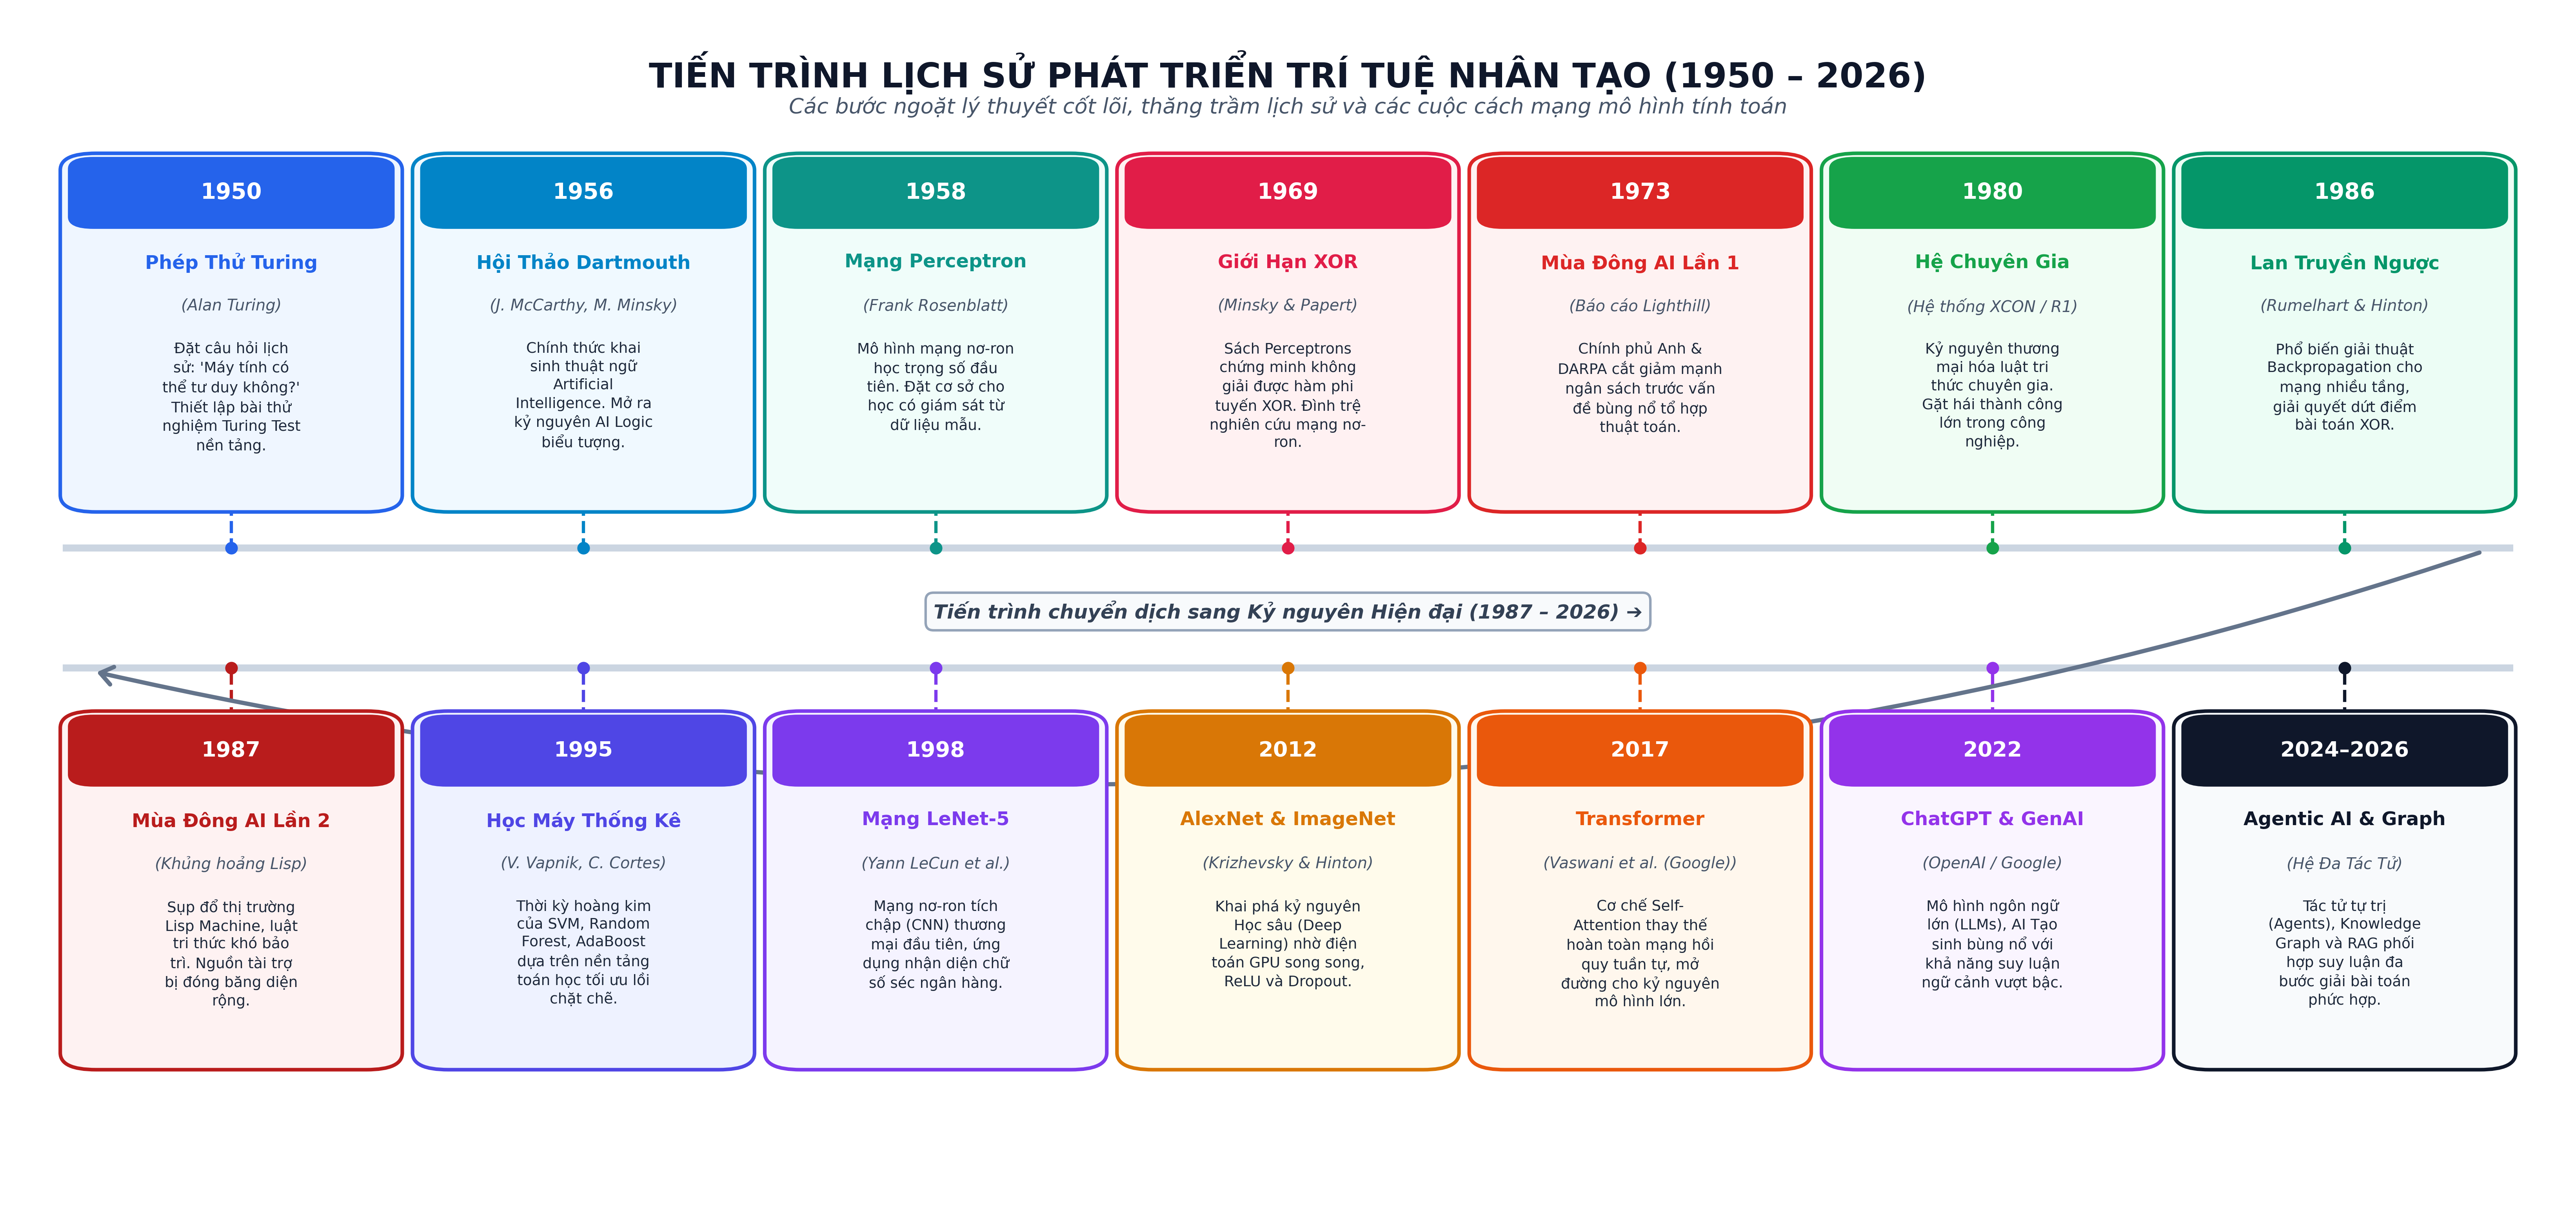
\includegraphics[width=\textwidth]{images/fig101_ai_evolution_timeline.png}
    \caption{Dòng thời gian tiến hóa Trí tuệ Nhân tạo (1950 -- 2026): Các mốc bước ngoặt lịch sử và sự chuyển dịch mô hình tính toán.}
    \label{fig:ai_timeline}
\end{figure}

Hình~\ref{fig:ai_timeline} tổng kết 15 cột mốc then chốt xác lập quỹ đạo phát triển của AI. Để thấu hiểu sâu sắc bản chất của các mô hình học máy và học sâu hiện đại, việc khảo cứu nguồn gốc lịch sử, các thất bại mang tính hệ thống trong quá khứ và động lực thúc đẩy các cuộc cách mạng công nghệ là một yêu cầu học thuật thiết yếu.

\section{Khởi Nguồn và Kỷ Nguyên Logic Biểu Tượng (1940s -- 1960s)}

\subsection{Ý Niệm Về Máy Tính Có Tư Duy và Phép Thử Turing}
Khởi nguồn lý thuyết của AI bắt đầu từ công trình kinh điển của nhà toán học Alan Turing vào năm 1950 với bài báo mang tựa đề \textit{“Computing Machinery and Intelligence”} đăng trên tạp chí \textit{Mind}. Trong công trình này, Turing đã đặt ra câu hỏi mang tính bản lề: \textit{“Máy móc có thể tư duy được hay không?”} (Can machines think?). Để tránh những tranh cãi trừu tượng về khái niệm ý thức và tư duy, ông đã đề xuất một phép thử thực nghiệm hành vi mang tên \textit{“Trò chơi bắt chước”} (The Imitation Game), ngày nay được biết đến rộng rãi với tên gọi \textbf{Phép thử Turing (Turing Test)}.

Theo tiêu chí của Turing, một cỗ máy được coi là có trí tuệ nếu trong một cuộc giao tiếp bằng văn bản được che giấu (blind text test), một người thẩm vấn bình thường không thể phân biệt được đối tượng đang trò chuyện là một con người hay là một chương trình máy tính. Dù còn nhiều tranh luận triết học, Phép thử Turing đã đặt nền móng phương pháp luận đầu tiên cho việc định lượng hóa hành vi thông minh nhân tạo.

\subsection{Mô Hình Nơ-ron Hình Thức và Hội Thảo Dartmouth (1956)}
Trước công trình của Turing, vào năm 1943, Warren McCulloch (nhà thần kinh học) và Walter Pitts (nhà logic học) đã công bố mô hình nơ-ron hình thức đầu tiên (McCulloch-Pitts Neuron). Họ đã chứng minh rằng các nơ-ron sinh học được đơn giản hóa có thể thực thi các phép toán logic cơ bản như AND, OR, NOT thông qua cơ chế tổng tích lũy tín hiệu đầu vào và so sánh với một ngưỡng kích hoạt:
\begin{equation}
y = f\left(\sum_{i=1}^n w_i x_i - \theta\right)
\end{equation}
trong đó $x_i \in \{0, 1\}$ là tín hiệu nhị phân đầu vào, $w_i$ là trọng số liên kết, $\theta$ là ngưỡng kích hoạt, và $f(\cdot)$ là hàm bước nhảy Heaviside. Đến năm 1949, Donald Hebb đề xuất quy tắc học Hebbian (\textit{“Neurons that fire together, wire together”}), đặt cơ sở cho việc thay đổi độ mạnh liên kết khớp thần kinh sinh học.

Bước ngoặt lịch sử chính thức khai sinh ra ngành khoa học Trí tuệ Nhân tạo diễn ra vào mùa hè năm 1956 tại \textbf{Hội thảo Dartmouth (Dartmouth Summer Research Project on Artificial Intelligence)} do John McCarthy (Đại học Dartmouth), Marvin Minsky (Đại học Harvard), Claude Shannon (Bell Labs) và Nathaniel Rochester (IBM) đồng tổ chức. Chính tại hội thảo này, John McCarthy đã đề xuất thuật ngữ \textbf{“Artificial Intelligence”} với mệnh đề cốt lõi: \textit{“Mọi khía cạnh của việc học hỏi hay bất kỳ đặc tính nào khác của trí tuệ về nguyên tắc đều có thể được mô tả chính xác đến mức một cỗ máy có thể được chế tạo để mô phỏng nó”}.

\subsection{Perceptron của Rosenblatt và Các Hệ Suy Diễn Ký Hiệu Đầu Tiên}
Năm 1957, Frank Rosenblatt tại Phòng thí nghiệm Hàng không Cornell đã chế tạo thành công mô hình phần cứng \textbf{Perceptron} trên máy tính IBM 704. Khác với nơ-ron McCulloch-Pitts vốn có trọng số cố định, Perceptron là mô hình nơ-ron nhân tạo đầu tiên có khả năng \textit{tự động học trọng số} từ dữ liệu mẫu thông qua thuật toán học có giám sát:
\begin{equation}
\mathbf{w}^{(t+1)} = \mathbf{w}^{(t)} + \eta (y - \hat{y}) \mathbf{x}
\end{equation}
với $\eta > 0$ là tốc độ học (learning rate), $y \in \{0, 1\}$ là nhãn thực tế và $\hat{y}$ là nhãn dự báo. Định lý hội tụ Perceptron (Perceptron Convergence Theorem) của Rosenblatt chứng minh rằng nếu tập dữ liệu khả phân tuyến tính (linearly separable), thuật toán chắc chắn sẽ hội tụ về một siêu phẳng phân tách sau một số hữu hạn các bước lặp.

Song song với hướng tiếp cận kết nối (connectionism) của Perceptron, nhánh tiếp cận biểu tượng (symbolic AI) cũng đạt được những thành tựu rực rỡ với \textit{Logic Theorist} (1956) của Allen Newell, Herbert Simon và Cliff Shaw -- chương trình máy tính đầu tiên chứng minh được 38 trên 52 định lý trong chương 2 cuốn \textit{Principia Mathematica} của Russell và Whitehead. Tiếp sau đó là chương trình \textit{General Problem Solver (GPS)} (1959) sử dụng kỹ thuật phân tích phương tiện -- cứu cánh (means-ends analysis) để giải quyết các bài toán giải đố hình thức.

\section{“Mùa Đông AI” Lần Thứ Nhất (1970s)}

\subsection{Giới Hạn Toán Học Của Perceptron và Cuốn Sách Của Minsky \& Papert (1969)}
Sự lạc quan tột độ trong thập niên 1960 nhanh chóng nhường chỗ cho một cuộc khủng hoảng học thuật sâu sắc. Năm 1969, Marvin Minsky và Seymour Papert xuất bản cuốn sách mang tính bước ngoặt \textbf{\textit{“Perceptrons: An Introduction to Computational Geometry”}}. Bằng các chứng minh hình học và đại số chặt chẽ, hai tác giả đã chỉ ra một hạn chế căn bản: \textbf{Perceptron đơn tầng không có khả năng giải quyết các bài toán phi tuyến tính cơ bản, điển hình là hàm logic XOR (Exclusive-OR)}.

\begin{table}[H]
\centering
\caption{Bảng chân lý hàm logic XOR chứng minh tính chất không khả phân tuyến tính}
\label{tab:xor_truth_table}
\begin{tabularx}{0.75\textwidth}{>{\centering\arraybackslash}X >{\centering\arraybackslash}X >{\centering\arraybackslash}X >{\raggedright\arraybackslash}X}
\toprule
\textbf{Đầu vào $x_1$} & \textbf{Đầu vào $x_2$} & \textbf{Đầu ra $y = x_1 \oplus x_2$} & \textbf{Vị trí hình học trên mặt phẳng $\mathbb{R}^2$} \\
\midrule
0 & 0 & 0 & Gốc tọa độ $(0, 0)$ -- Nhãn âm \\
0 & 1 & 1 & Điểm $(0, 1)$ -- Nhãn dương \\
1 & 0 & 1 & Điểm $(1, 0)$ -- Nhãn dương \\
1 & 1 & 0 & Điểm $(1, 1)$ -- Nhãn âm \\
\bottomrule
\end{tabularx}
\end{table}

Để phân tách nhãn dương $\{ (0,1), (1,0) \}$ khỏi nhãn âm $\{ (0,0), (1,1) \}$, không tồn tại bất kỳ một đường thẳng nào dạng $w_1 x_1 + w_2 x_2 + b = 0$ có thể chia đôi mặt phẳng sao cho hai nhóm điểm nằm về hai phía đối lập. Mặc dù Minsky và Papert thừa nhận rằng mạng nơ-ron nhiều tầng (multilayer networks) có thể giải quyết được bài toán phi tuyến tính, nhưng vào thời điểm đó, chưa một ai tìm ra được giải thuật toán học hiệu quả để huấn luyện các trọng số ở các tầng ẩn (hidden layers). Cuốn sách đã giáng một đòn chí mạng vào cộng đồng nghiên cứu mạng nơ-ron, khiến các cơ quan tài trợ gần như đóng băng toàn bộ nguồn lực dành cho hướng tiếp cận kết nối.

\subsection{Báo Cáo Lighthill (1973) và Sự Cắt Giảm Tài Trợ Của DARPA}
Tại Vương quốc Anh, Hội đồng Nghiên cứu Khoa học (SRC) đã ủy quyền cho Giáo sư James Lighthill tiến hành đánh giá độc lập về thực trạng nghiên cứu AI. Năm 1973, \textbf{Báo cáo Lighthill (Lighthill Report)} được công bố với những kết luận vô cùng bi quan. Lighthill chỉ ra rằng các hệ thống AI biểu tượng chỉ hoạt động được trong các “thế giới đồ chơi” (toy worlds) vô cùng hạn hẹp và hoàn toàn bất lực trước các bài toán thực tế do hiện tượng \textbf{bùng nổ tổ hợp (combinatorial explosion)}. Số lượng trạng thái tìm kiếm tăng theo hàm mũ đối với kích thước bài toán, vượt xa khả năng xử lý của mọi hệ thống máy tính đương thời.

Báo cáo Lighthill đã dẫn đến việc chính phủ Anh chấm dứt tài trợ nghiên cứu AI tại hầu hết các trường đại học (ngoại trừ Edinburgh, Sussex và Essex). Cùng thời điểm đó tại Hoa Kỳ, Cơ quan Chỉ đạo các Dự án Nghiên cứu Tiên tiến Quốc phòng (DARPA) cũng áp dụng Đạo luật Mansfield, cắt giảm các khoản tài trợ cho nghiên cứu cơ bản không có ứng dụng quân sự trực tiếp. Giai đoạn 1974 -- 1980 chính thức đi vào lịch sử với tên gọi \textbf{“Mùa đông AI lần thứ nhất”}.

\section{Sự Trỗi Dậy Của Hệ Chuyên Gia và “Mùa Đông AI” Lần Thứ Hai (1980s -- 1990s)}

\subsection{Kỷ Nguyên Vàng Của Hệ Chuyên Gia (Expert Systems)}
Đầu thập niên 1980, AI phục hưng mạnh mẽ nhờ sự chuyển dịch từ tìm kiếm tổng quát sang biểu diễn tri thức chuyên gia trong các miền hẹp (domain-specific knowledge). Đây là thời kỳ hoàng kim của \textbf{Hệ Chuyên gia (Expert Systems)}. Khác với các thuật toán tối ưu toán học, hệ chuyên gia mô phỏng quá trình ra quyết định của các chuyên gia con người thông qua việc tách biệt rõ ràng giữa hai thành phần:
\begin{enumerate}[leftmargin=1.2cm]
    \item \textbf{Cơ sở tri thức (Knowledge Base):} Lưu trữ các sự kiện và tập luật dưới dạng các mệnh đề điều kiện \texttt{IF <điều kiện> THEN <hành động/kết luận>}.
    \item \textbf{Máy suy diễn (Inference Engine):} Động cơ thực thi logic, vận hành theo cơ chế suy diễn tiến (Forward Chaining -- từ dữ kiện suy ra kết luận) hoặc suy diễn lùi (Backward Chaining -- từ giả thuyết truy ngược về dữ kiện cần chứng minh).
\end{enumerate}

Các hệ chuyên gia tiêu biểu giai đoạn này bao gồm:
\begin{itemize}[leftmargin=1.2cm]
    \item \textbf{DENDRAL (Đại học Stanford):} Phân tích phổ khối lượng để xác định cấu trúc phân tử hóa học hữu cơ.
    \item \textbf{MYCIN (Đại học Stanford):} Chẩn đoán các bệnh nhiễm trùng máu và đề xuất phác đồ kháng sinh, đạt tỷ lệ chẩn đoán chính xác tương đương các bác sĩ chuyên khoa hàng đầu.
    \item \textbf{XCON / R1 (Đại học Carnegie Mellon \& Digital Equipment Corporation - DEC):} Hệ thống thương mại hóa thành công rực rỡ nhất, tự động cấu hình các hệ thống máy tính VAX theo đơn đặt hàng của khách hàng, giúp DEC tiết kiệm ước tính hơn 40 triệu USD mỗi năm vào năm 1986.
\end{itemize}

Sự thành công của XCON đã châm ngòi cho một làn sóng đầu tư thương mại khổng lồ vào các công ty khởi nghiệp phần cứng chuyên dụng chạy ngôn ngữ Lisp (Lisp Machines như Symbolics, LMI) và các dự án quốc gia quy mô lớn như Dự án Máy tính Thế hệ thứ Năm (Fifth Generation Computer Systems - FGCS) của Nhật Bản với ngân sách hàng trăm triệu USD.

\subsection{Sự Tái Sinh Của Mạng Nơ-ron: Giải Thuật Lan Truyền Ngược (1986)}
Trong khi hệ chuyên gia thống trị về mặt thương mại, hướng tiếp cận mạng nơ-ron đã âm thầm tạo nên bước đột phá khoa học quan trọng nhất của thế kỷ 20. Năm 1986, David Rumelhart, Geoffrey Hinton và Ronald Williams đã công bố bài báo lịch sử trên tạp chí \textit{Nature}: \textit{“Learning representations by back-propagating errors”}.

Công trình này đã phổ biến rộng rãi giải thuật \textbf{Lan truyền ngược (Backpropagation)} cho mạng nơ-ron đa tầng (Multilayer Perceptron -- MLP). Bằng cách áp dụng quy tắc dây chuyền của giải tích vi phân (chain rule of calculus) kết hợp với các hàm kích hoạt phi tuyến khả vi liên tục (như hàm Sigmoid $\sigma(z) = \frac{1}{1 + e^{-z}}$), giải thuật cho phép tính toán đạo hàm riêng của hàm mất mát $L$ đối với từng trọng số ở bất kỳ tầng ẩn nào trong mạng:
\begin{equation}
\frac{\partial L}{\partial w_{ij}^{(l)}} = \delta_i^{(l)} \cdot a_j^{(l-1)}
\end{equation}
với $\delta_i^{(l)}$ là sai số truyền ngược tại nơ-ron $i$ của tầng $l$, và $a_j^{(l-1)}$ là giá trị kích hoạt của nơ-ron $j$ tại tầng trước đó. Đột phá này đã phá vỡ hoàn toàn “lời nguyền XOR” của Minsky và Papert, chứng minh rằng mạng nơ-ron hoàn toàn có thể tự động học các biểu diễn đặc trưng ẩn phi tuyến tính phức tạp. Cũng trong giai đoạn này, Kunihiko Fukushima (1980) công bố mô hình \textbf{Neocognitron}, đưa ra khái niệm xếp chồng các tầng trích xuất đặc trưng (S-cells) và tầng bất biến vị trí (C-cells), đặt nền tảng kiến trúc trực tiếp cho Mạng nơ-ron Tích chập (CNN) sau này.

\subsection{“Mùa Đông AI” Lần Thứ Hai (1987 -- 1993)}
Tuy nhiên, sự bùng nổ thương mại của hệ chuyên gia nhanh chóng bộc lộ những rạn nứt cấu trúc nghiêm trọng:
\begin{itemize}[leftmargin=1.2cm]
    \item \textbf{Điểm nghẽn thu nhận tri thức (Knowledge Acquisition Bottleneck):} Việc phỏng vấn các chuyên gia con người để mã hóa tri thức thành hàng vạn luật logic là một quá trình cực kỳ tốn kém, chậm chạp và dễ phát sinh mâu thuẫn.
    \item \textbf{Tính giòn (Brittleness) và Khủng hoảng bảo trì:} Khi cơ sở tri thức tăng lên quy mô hàng chục nghìn luật, sự tương tác phức tạp giữa các luật dẫn đến các vòng lặp vô tận hoặc kết luận sai lệch khi gặp các tình huống nằm ngoài biên tri thức đã định nghĩa. Chi phí bảo trì hệ thống vượt xa lợi ích kinh tế mang lại.
    \item \textbf{Sự sụp đổ của thị trường phần cứng Lisp:} Cuối thập niên 1980, sự phát triển vượt bậc của vi xử lý thông dụng x86 (Intel 386, 486) và các máy trạm Unix (Sun Microsystems) đã khiến các máy tính chuyên dụng Lisp Machines đắt đỏ trở nên lỗi thời về hiệu năng trên chi phí. Thị trường Lisp sụp đổ kéo theo hàng loạt công ty AI phá sản.
\end{itemize}

Cuộc khủng hoảng này đã mở ra \textbf{“Mùa đông AI lần thứ hai”} kéo dài từ 1987 đến đầu thập niên 1990.

\begin{figure}[H]
    \centering
    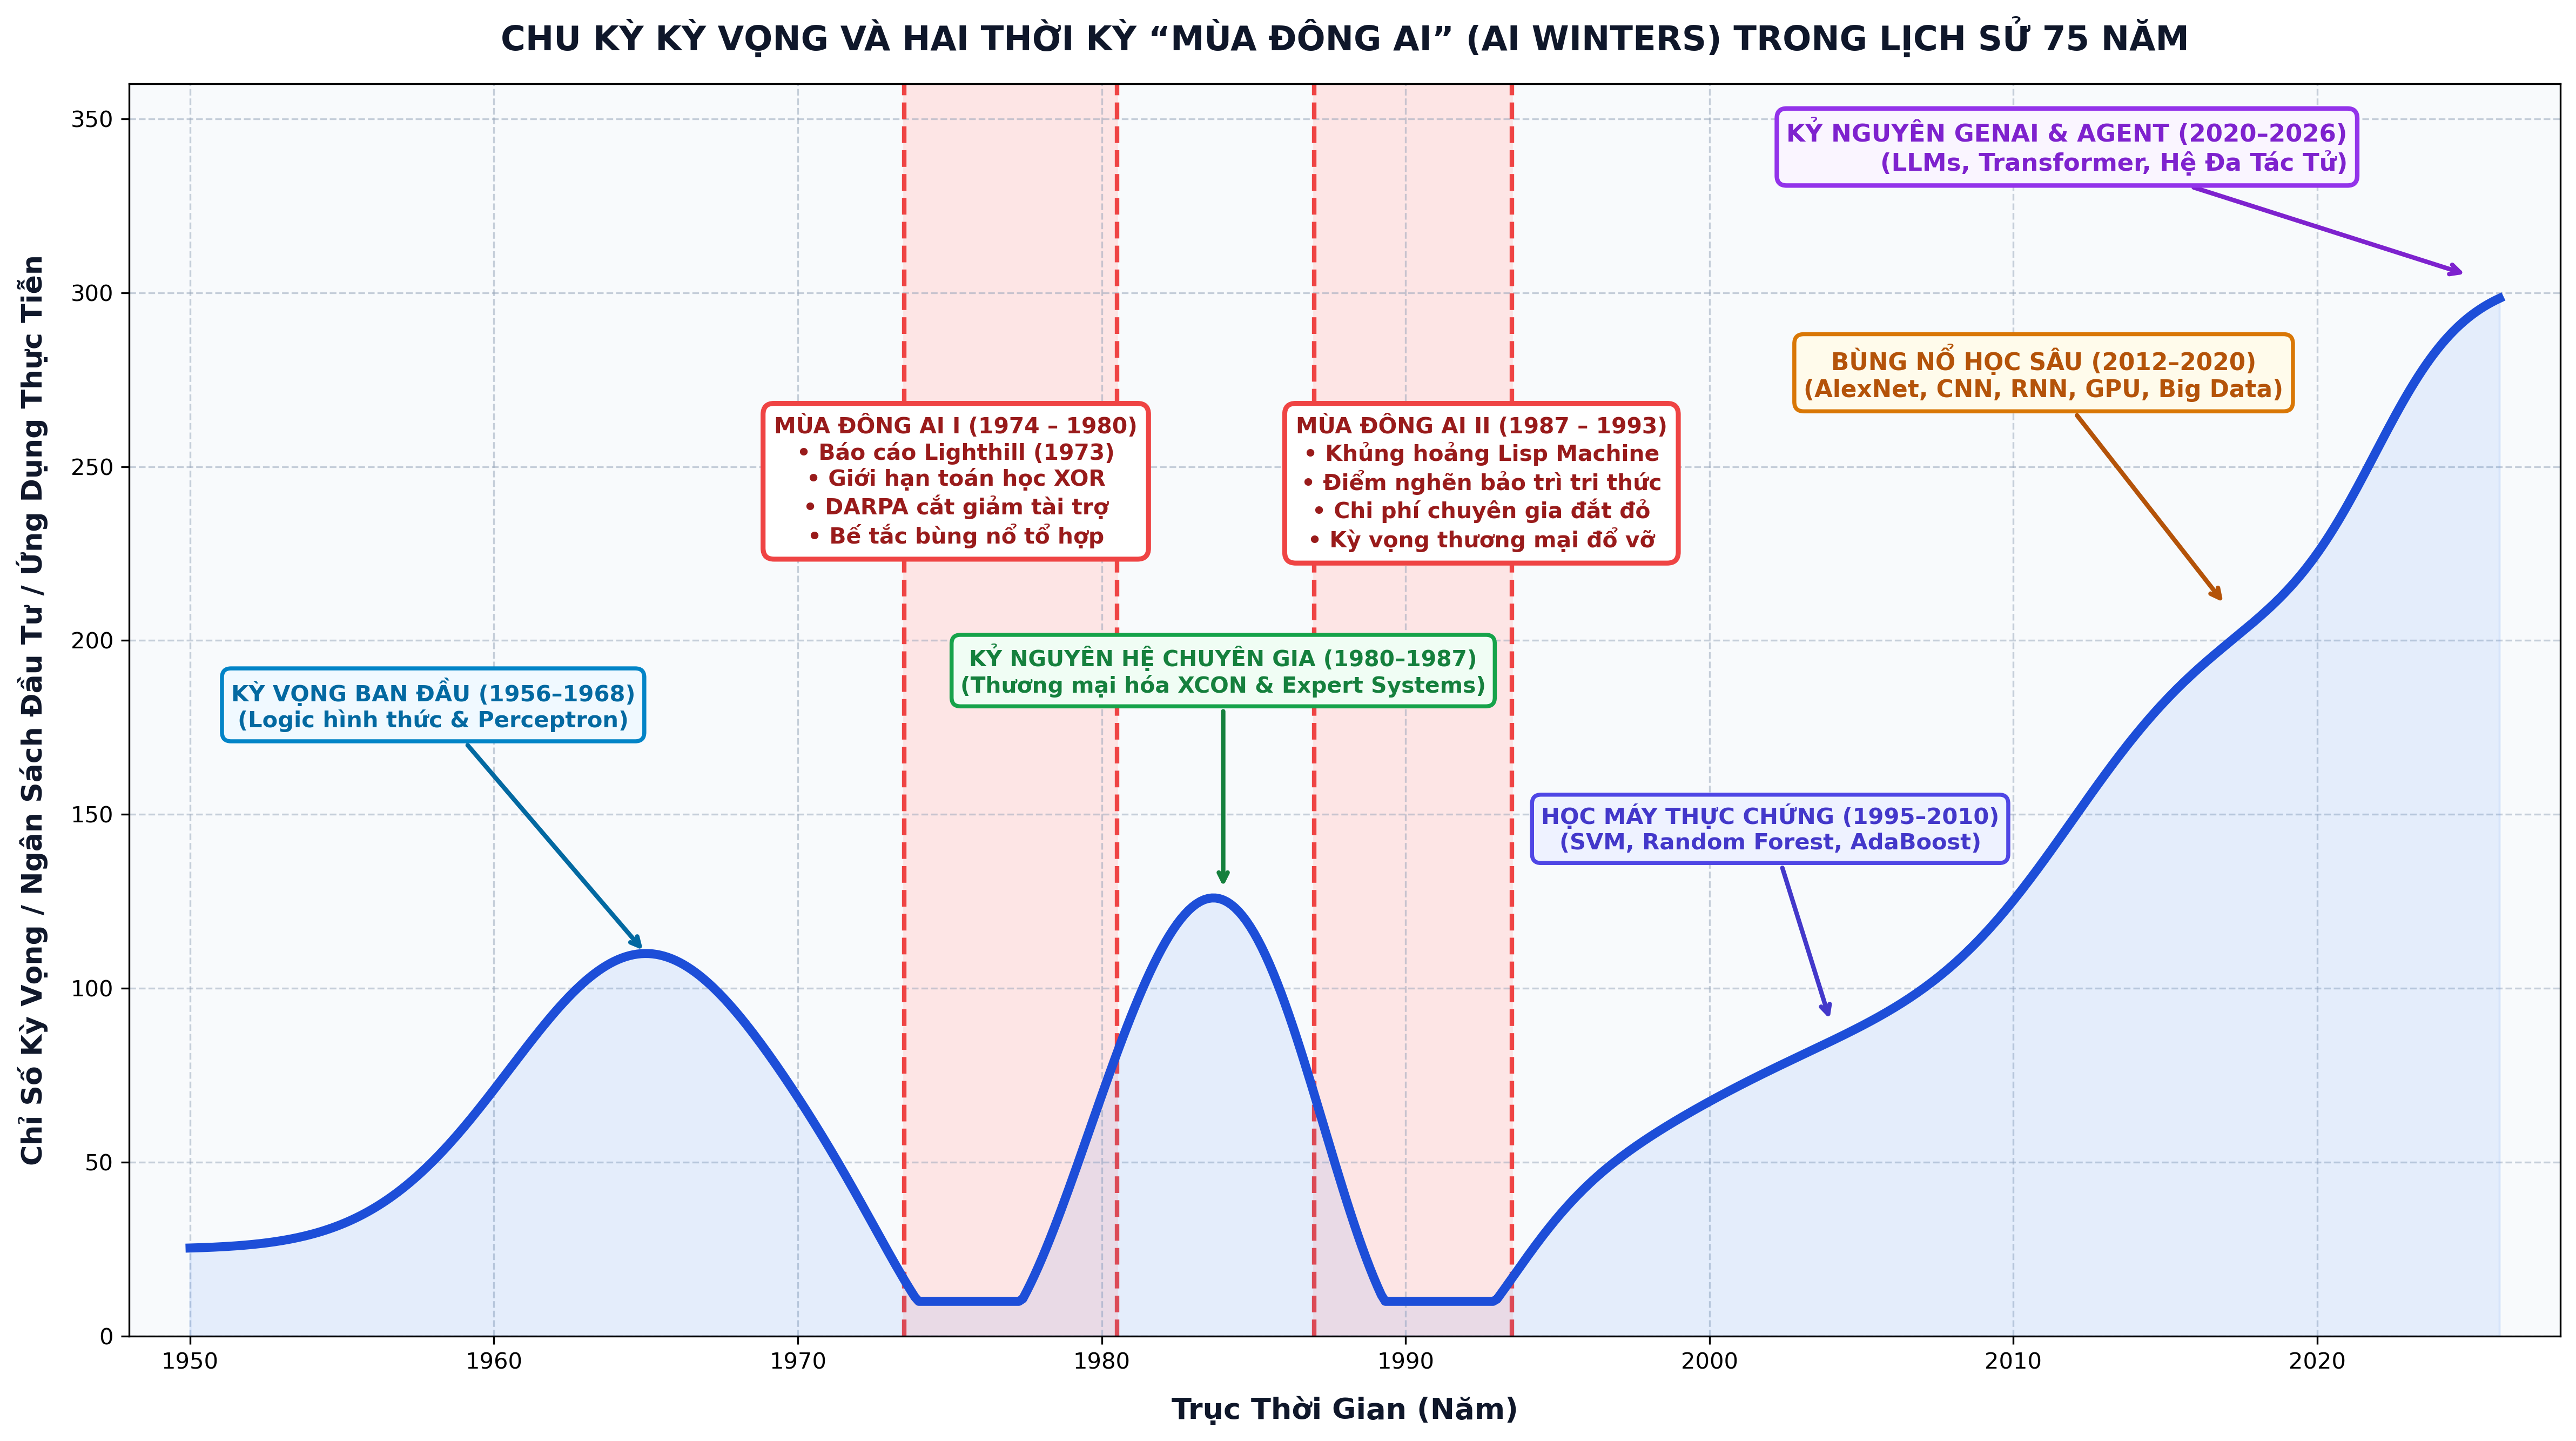
\includegraphics[width=\textwidth]{images/fig102_ai_winters_and_hype_cycles.png}
    \caption{Chu kỳ kỳ vọng và hai thời kỳ “Mùa đông AI” (AI Winters) trong tiến trình 75 năm lịch sử.}
    \label{fig:ai_winters}
\end{figure}

Hình~\ref{fig:ai_winters} trực quan hóa các chu kỳ kỳ vọng (Hype Cycles) và hai giai đoạn “Mùa đông AI”. Đồ thị cho thấy sau mỗi cuộc khủng hoảng thoái trào, cộng đồng khoa học lại tái cấu trúc nền tảng phương pháp luận, chuyển dịch sang các mô hình thực dụng và có cơ sở toán học vững chắc hơn.

\section{Kỷ Nguyên Học Máy Thống Kê Thực Nghiệm (1990s -- 2010)}

Sau thất bại của các hệ chuyên gia dựa trên luật, cộng đồng AI đã rút ra một bài học sống còn: \textbf{Thay vì cố gắng lập trình thủ công toàn bộ các quy tắc tri thức phức tạp của thế giới, hãy để máy tính tự học các quy luật xác suất thống kê trực tiếp từ dữ liệu thực nghiệm}.

\subsection{Lý Thuyết Học Thống Kê và Máy Vector Hỗ Trợ (SVM)}
Thập niên 1990 chứng kiến sự trỗi dậy áp đảo của \textbf{Lý thuyết Học Thống kê (Statistical Learning Theory)} do Vladimir Vapnik và Alexey Chervonenkis hoàn thiện. Trọng tâm của lý thuyết này là nguyên lý Cực tiểu hóa Rủi ro Cấu trúc (Structural Risk Minimization -- SRM), nhằm kiểm soát sự cân bằng giữa sai số trên tập huấn luyện và năng lực khái quát hóa thông qua chiều VC (Vapnik-Chervonenkis Dimension).

Đỉnh cao của giai đoạn này là sự ra đời của \textbf{Máy Vector Hỗ trợ (Support Vector Machines -- SVM)} (Boser, Guyon \& Vapnik, 1992; Cortes \& Vapnik, 1995). Khác với Perceptron vốn tìm bất kỳ mặt phân cách nào, SVM tìm kiếm siêu phẳng tối ưu có khoảng cách biên (margin) lớn nhất tới các điểm dữ liệu gần nhất (support vectors):
\begin{equation}
\min_{\mathbf{w}, b} \frac{1}{2} \|\mathbf{w}\|^2 \quad \text{thỏa mãn} \quad y_i (\mathbf{w}^T \mathbf{x}_i + b) \ge 1, \quad \forall i
\end{equation}
Đặc biệt, thông qua \textbf{Kỹ thuật biến đổi hàm nhân (Kernel Trick)} (Mercer's Theorem), SVM cho phép ánh xạ ngầm các vector dữ liệu vào không gian đặc trưng vô hạn chiều (với nhân RBF Gaussian: $K(\mathbf{x}, \mathbf{x}') = \exp(-\gamma \|\mathbf{x} - \mathbf{x}'\|^2)$) để giải quyết các bài toán phi tuyến tính phức tạp mà không làm gia tăng độ phức tạp tính toán. Với nền tảng toán học tối ưu hóa lồi toàn cục (Convex Optimization) tuyệt đối không rơi vào cực tiểu cục bộ, SVM đã đánh bại hoàn toàn mạng nơ-ron đa tầng trên hầu hết các bài toán thị giác và phân loại văn bản trong suốt hơn một thập kỷ.

\subsection{Cây Quyết Định và Các Phương Pháp Học Tập Hợp (Ensemble Learning)}
Bên cạnh SVM, các phương pháp học tập hợp (Ensemble Learning) cũng xác lập vị thế thống trị trên dữ liệu bảng:
\begin{itemize}[leftmargin=1.2cm]
    \item \textbf{Cây quyết định (Decision Trees):} Các thuật toán CART (Breiman et al., 1984) và C4.5 (Quinlan, 1993) cung cấp khả năng diễn giải trực quan dựa trên chỉ số tạp chất Gini và độ lợi thông tin (Information Gain).
    \item \textbf{Boosting (AdaBoost):} Yoav Freund và Robert Schapire (1996) đề xuất giải thuật AdaBoost, chứng minh định lý toán học rằng có thể kết hợp tuyến tính nhiều bộ phân loại yếu (weak learners) để tạo thành một bộ phân loại mạnh (strong learner). Sau đó, Jerome Friedman (2001) tổng quát hóa thành Gradient Boosting Machine (GBM).
    \item \textbf{Rừng ngẫu nhiên (Random Forest):} Leo Breiman (2001) kết hợp kỹ thuật lấy mẫu lặp lại (Bootstrap Aggregating -- Bagging) với việc chọn tập con đặc trưng ngẫu nhiên (Random Feature Subsampling) để giảm phương sai (variance) của mô hình cây mà không làm tăng độ chệch (bias), tạo ra thuật toán học máy mạnh mẽ và ổn định nhất cho dữ liệu cấu trúc bảng.
\end{itemize}

\subsection{LeNet-5 (1998) -- Nền Tảng Của Mạng Tích Chập Hiện Đại}
Năm 1998, Yann LeCun cùng các cộng sự tại AT\&T Bell Labs đã công bố bài báo lịch sử \textit{“Gradient-based learning applied to document recognition”}, giới thiệu kiến trúc \textbf{LeNet-5}. LeNet-5 tích hợp hoàn chỉnh ba ý tưởng kiến trúc cốt lõi:
\begin{enumerate}[leftmargin=1.2cm]
    \item \textbf{Vùng tiếp nhận cục bộ (Local Receptive Fields):} Nơ-ron chỉ kết nối với một vùng lân cận không gian nhỏ của ảnh đầu vào.
    \item \textbf{Chia sẻ trọng số (Shared Weights):} Một bộ lọc (filter) quét qua toàn bộ ảnh, giảm mạnh số lượng tham số tự do và tạo tính bất biến tịnh tiến.
    \item \textbf{Lấy mẫu giảm dần (Sub-sampling / Pooling):} Giảm độ phân giải không gian của bản đồ đặc trưng, tăng cường khả năng chống nhiễu dịch chuyển và co dãn hình học.
\end{enumerate}
LeNet-5 đã được triển khai thương mại hóa thành công rực rỡ, xử lý hàng triệu tờ séc ngân hàng mỗi ngày trên khắp hệ thống ngân hàng Hoa Kỳ. Tuy nhiên, do giới hạn về năng lực tính toán của CPU và sự thiếu hụt các tập dữ liệu ảnh quy mô lớn vào thời điểm đó, mô hình này chưa thể mở rộng ra các bài toán nhận dạng ảnh tự nhiên phức tạp hơn.

\section{Cuộc Cách Mạng Học Sâu (Deep Learning Boom, 2012 -- 2020)}

\subsection{Bước Ngoặt Lịch Sử ImageNet 2012 và AlexNet}
Năm 2012 được ghi nhận là mốc khởi đầu của cuộc cách mạng học sâu hiện đại. Tại cuộc thi nhận dạng hình ảnh quy mô lớn thế giới \textbf{ImageNet Large Scale Visual Recognition Challenge (ILSVRC 2012)}, nhóm nghiên cứu của Đại học Toronto gồm Alex Krizhevsky, Ilya Sutskever và Geoffrey Hinton đã giới thiệu mô hình mạng nơ-ron tích chập sâu mang tên \textbf{AlexNet}.

Kết quả thi đấu đã gây chấn động toàn bộ cộng đồng khoa học máy tính: AlexNet đạt tỷ lệ sai số Top-5 là \textbf{15.3\%}, bỏ xa mô hình đứng thứ hai (sử dụng phương pháp học máy truyền thống kết hợp trích xuất đặc trưng thủ công SIFT/HOG + SVM) với sai số \textbf{26.2\%}. Mức chênh lệch hơn 10.9\% sai số tuyệt đối đã chứng minh tính ưu việt áp đảo của việc học biểu diễn tự động (end-to-end representation learning) so với kỹ nghệ đặc trưng thủ công (hand-crafted feature engineering).

Cuộc cách mạng này được thúc đẩy bởi sự hội tụ đồng thời của \textbf{“Bộ ba trụ cột” (The Holy Trinity of Deep Learning)}:
\begin{enumerate}[leftmargin=1.2cm]
    \item \textbf{Dữ liệu quy mô lớn (Big Data):} Tập dữ liệu ImageNet do Fei-Fei Li và cộng sự xây dựng chứa hơn 1.2 triệu ảnh có gán nhãn thuộc 1,000 phân lớp đối tượng tự nhiên khác nhau, cung cấp đủ bằng chứng thống kê để huấn luyện hàng chục triệu tham số mà không bị quá khớp nghiêm trọng.
    \item \textbf{Năng lực tính toán song song (Massive Parallel Hardware):} Việc ứng dụng GPU (Graphics Processing Units) của NVIDIA kết hợp nền tảng lập trình CUDA đã tăng tốc độ nhân ma trận lên hàng chục lần so với CPU truyền thống, cho phép huấn luyện mạng sâu 8 tầng với 60 triệu tham số trong vòng vài ngày thay vì hàng tháng.
    \item \textbf{Đột phá giải thuật tối ưu hóa và kích hoạt:}
    \begin{itemize}
        \item \textit{Hàm kích hoạt ReLU (Rectified Linear Unit) $f(x) = \max(0, x)$:} Thay thế hàm Sigmoid/Tanh, triệt tiêu hiện tượng bão hòa đạo hàm ở vùng dương, giúp tốc độ huấn luyện hội tụ nhanh hơn gấp 6 lần.
        \item \textit{Kỹ thuật điều chuẩn Dropout (Hinton et al., 2012):} Ngẫu nhiên vô hiệu hóa một tỷ lệ nơ-ron trong quá trình lan truyền tiến, phá vỡ sự phụ thuộc đồng biến phức tạp (co-adaptation) giữa các nơ-ron, ngăn ngừa quá khớp hiệu quả.
    \end{itemize}
\end{enumerate}

\subsection{Sự Tiến Hóa Của Các Kiến Trúc Thị Giác: VGG, ResNet, MobileNet}
Sau AlexNet, cộng đồng nghiên cứu bước vào cuộc chạy đua thiết kế kiến trúc mạng nơ-ron sâu hơn và hiệu quả hơn:
\begin{itemize}[leftmargin=1.2cm]
    \item \textbf{VGGNet (Simonyan \& Zisserman, 2014):} Chuẩn hóa nguyên lý thiết kế mô-đun hóa: thay vì dùng các bộ lọc lớn ($11 \times 11$ hay $5 \times 5$), VGG xếp chồng liên tiếp các bộ lọc tích chập siêu nhỏ kích thước $3 \times 3$. Hai tầng $3 \times 3$ liên tiếp có cùng vùng cảm nhận hiệu dụng ($5 \times 5$) nhưng giảm được $28\%$ số lượng tham số và tăng tính phi tuyến thông qua hai hàm kích hoạt ReLU.
    \item \textbf{ResNet (He et al., 2015 -- Đạt giải nhất ILSVRC 2015):} Khi chiều sâu của mạng vượt quá 20 tầng, hiện tượng thoái hóa mạng (degradation problem) xuất hiện khiến sai số huấn luyện tăng vọt (không phải do quá khớp). Kaiming He và các cộng sự đã đề xuất khối \textbf{Kết nối phần dư (Residual Block / Skip Connection)}:
    \begin{equation}
    \mathbf{y} = \mathcal{F}(\mathbf{x}, \{W_i\}) + \mathbf{x}
    \end{equation}
    Bằng cách cho phép tín hiệu đầu vào $\mathbf{x}$ cộng trực tiếp vào đầu ra của các tầng biến đổi, gradient trong quá trình lan truyền ngược có thể chảy trực tiếp qua kết nối tắt mà không bị suy hao. Đột phá này cho phép huấn luyện thành công các mạng có độ sâu chưa từng có (lên tới 152 tầng và thậm chí 1,000 tầng), đưa tỷ lệ lỗi phân loại ảnh ImageNet xuống \textbf{3.57\%}, chính thức vượt qua ngưỡng chính xác của mắt người ($5.1\%$).
    \item \textbf{MobileNet (Howard et al., 2017):} Tối ưu hóa tính toán cho các thiết bị nhúng và di động biên (Edge AI) thông qua kỹ thuật \textbf{Tích chập tách biệt chiều sâu (Depthwise Separable Convolution)}, phân rã phép tích chập chuẩn thành hai bước độc lập: Depthwise Conv (lọc không gian) và Pointwise Conv $1 \times 1$ (kết hợp kênh), giúp giảm chi phí tính toán FLOPs từ 8 đến 9 lần mà độ chính xác chỉ suy giảm nhẹ.
\end{itemize}

\subsection{Mô Hình Hóa Chuỗi: Từ RNN, LSTM Đến Cuộc Cách Mạng Transformer}
Song song với thị giác máy tính, việc xử lý dữ liệu chuỗi tuần tự (Sequential Data) như ngôn ngữ tự nhiên và chuỗi thời gian tài chính cũng có những bước chuyển mình căn bản:
\begin{itemize}[leftmargin=1.2cm]
    \item \textbf{RNN và Rào cản triệt tiêu đạo hàm:} Mạng nơ-ron hồi quy (Simple RNN) sử dụng trạng thái ẩn hồi quy để duy trì bộ nhớ chuỗi. Tuy nhiên, giải thuật lan truyền ngược qua thời gian (BPTT) gặp rào cản toán học nghiêm trọng: tích liên tiếp các ma trận chuyển trạng thái khiến gradient suy giảm theo hàm mũ, dẫn đến hiện tượng triệt tiêu đạo hàm (vanishing gradient), khiến mô hình không thể học được phụ thuộc dài hạn.
    \item \textbf{LSTM và GRU:} Kiến trúc \textbf{LSTM} (Hochreiter \& Schmidhuber, 1997) giải quyết triệt để vấn đề này nhờ cơ chế đường cao tốc ô nhớ trạng thái (Cell State) được điều khiển bởi 3 cổng tuyến tính: Cổng Quên (Forget Gate), Cổng Vào (Input Gate), và Cổng Ra (Output Gate). Biến thể \textbf{GRU} (Cho et al., 2014) tinh gọn kiến trúc xuống còn 2 cổng (Reset và Update), giúp tối ưu hóa tốc độ huấn luyện.
    \item \textbf{Transformer (2017):} Dù LSTM và GRU thống trị suốt hai thập kỷ, bản chất tính toán tuần tự từng bước thời gian của mạng hồi quy ngăn cản việc tính toán song song hóa trên quy mô lớn của GPU. Năm 2017, Vaswani và các cộng sự tại Google công bố bài báo lịch sử mang tựa đề \textbf{\textit{“Attention Is All You Need”}}, giới thiệu kiến trúc \textbf{Transformer}. Bằng cách loại bỏ hoàn toàn các liên kết hồi quy và dựa hoàn toàn vào \textbf{Cơ chế Tự chú ý đa đầu (Multi-Head Self-Attention)}, Transformer cho phép mô hình nắm bắt tương quan giữa mọi vị trí trong chuỗi với độ phức tạp đường dẫn là $O(1)$ và hỗ trợ song song hóa tuyệt đối, mở ra kỷ nguyên của các mô hình ngôn ngữ khổng lồ.
\end{itemize}

\section{Kỷ Nguyên AI Tạo Sinh, Mô Hình Nền Tảng và Xu Hướng Hệ Đa Agent (2020 -- Hiện Nay)}

\subsection{Mô Hình Ngôn Ngữ Lớn (LLMs) và Định Luật Tỷ Lệ (Scaling Laws)}
Từ năm 2020 đến nay, thế giới chứng kiến sự bùng nổ của kỷ nguyên \textbf{AI Tạo sinh (Generative AI)} và các \textbf{Mô hình Nền tảng (Foundation Models)}. Các nghiên cứu của Kaplan et al. (2020) và Chinchilla (Hoffmann et al., 2022) đã xác lập các \textbf{Định luật Tỷ lệ (Scaling Laws)}: hiệu năng của các mô hình ngôn ngữ tuân theo hàm lũy thừa chặt chẽ đối với ba yếu tố: số lượng tham số mô hình, kích thước tập dữ liệu huấn luyện và ngân sách tính toán (FLOPs).

Khi mô hình đạt quy mô hàng trăm tỷ tham số (như GPT-3, GPT-4 của OpenAI; Llama của Meta; Gemini của Google), các \textbf{năng lực nổi trội (Emergent Abilities)} xuất hiện: khả năng học trong ngữ cảnh mà không cần cập nhật trọng số (In-Context Few-Shot Learning), tư duy giải quyết vấn đề từng bước thông qua chuỗi suy luận (Chain-of-Thought Prompting), và năng lực sinh mã nguồn lập trình chuẩn xác.

\begin{figure}[H]
    \centering
    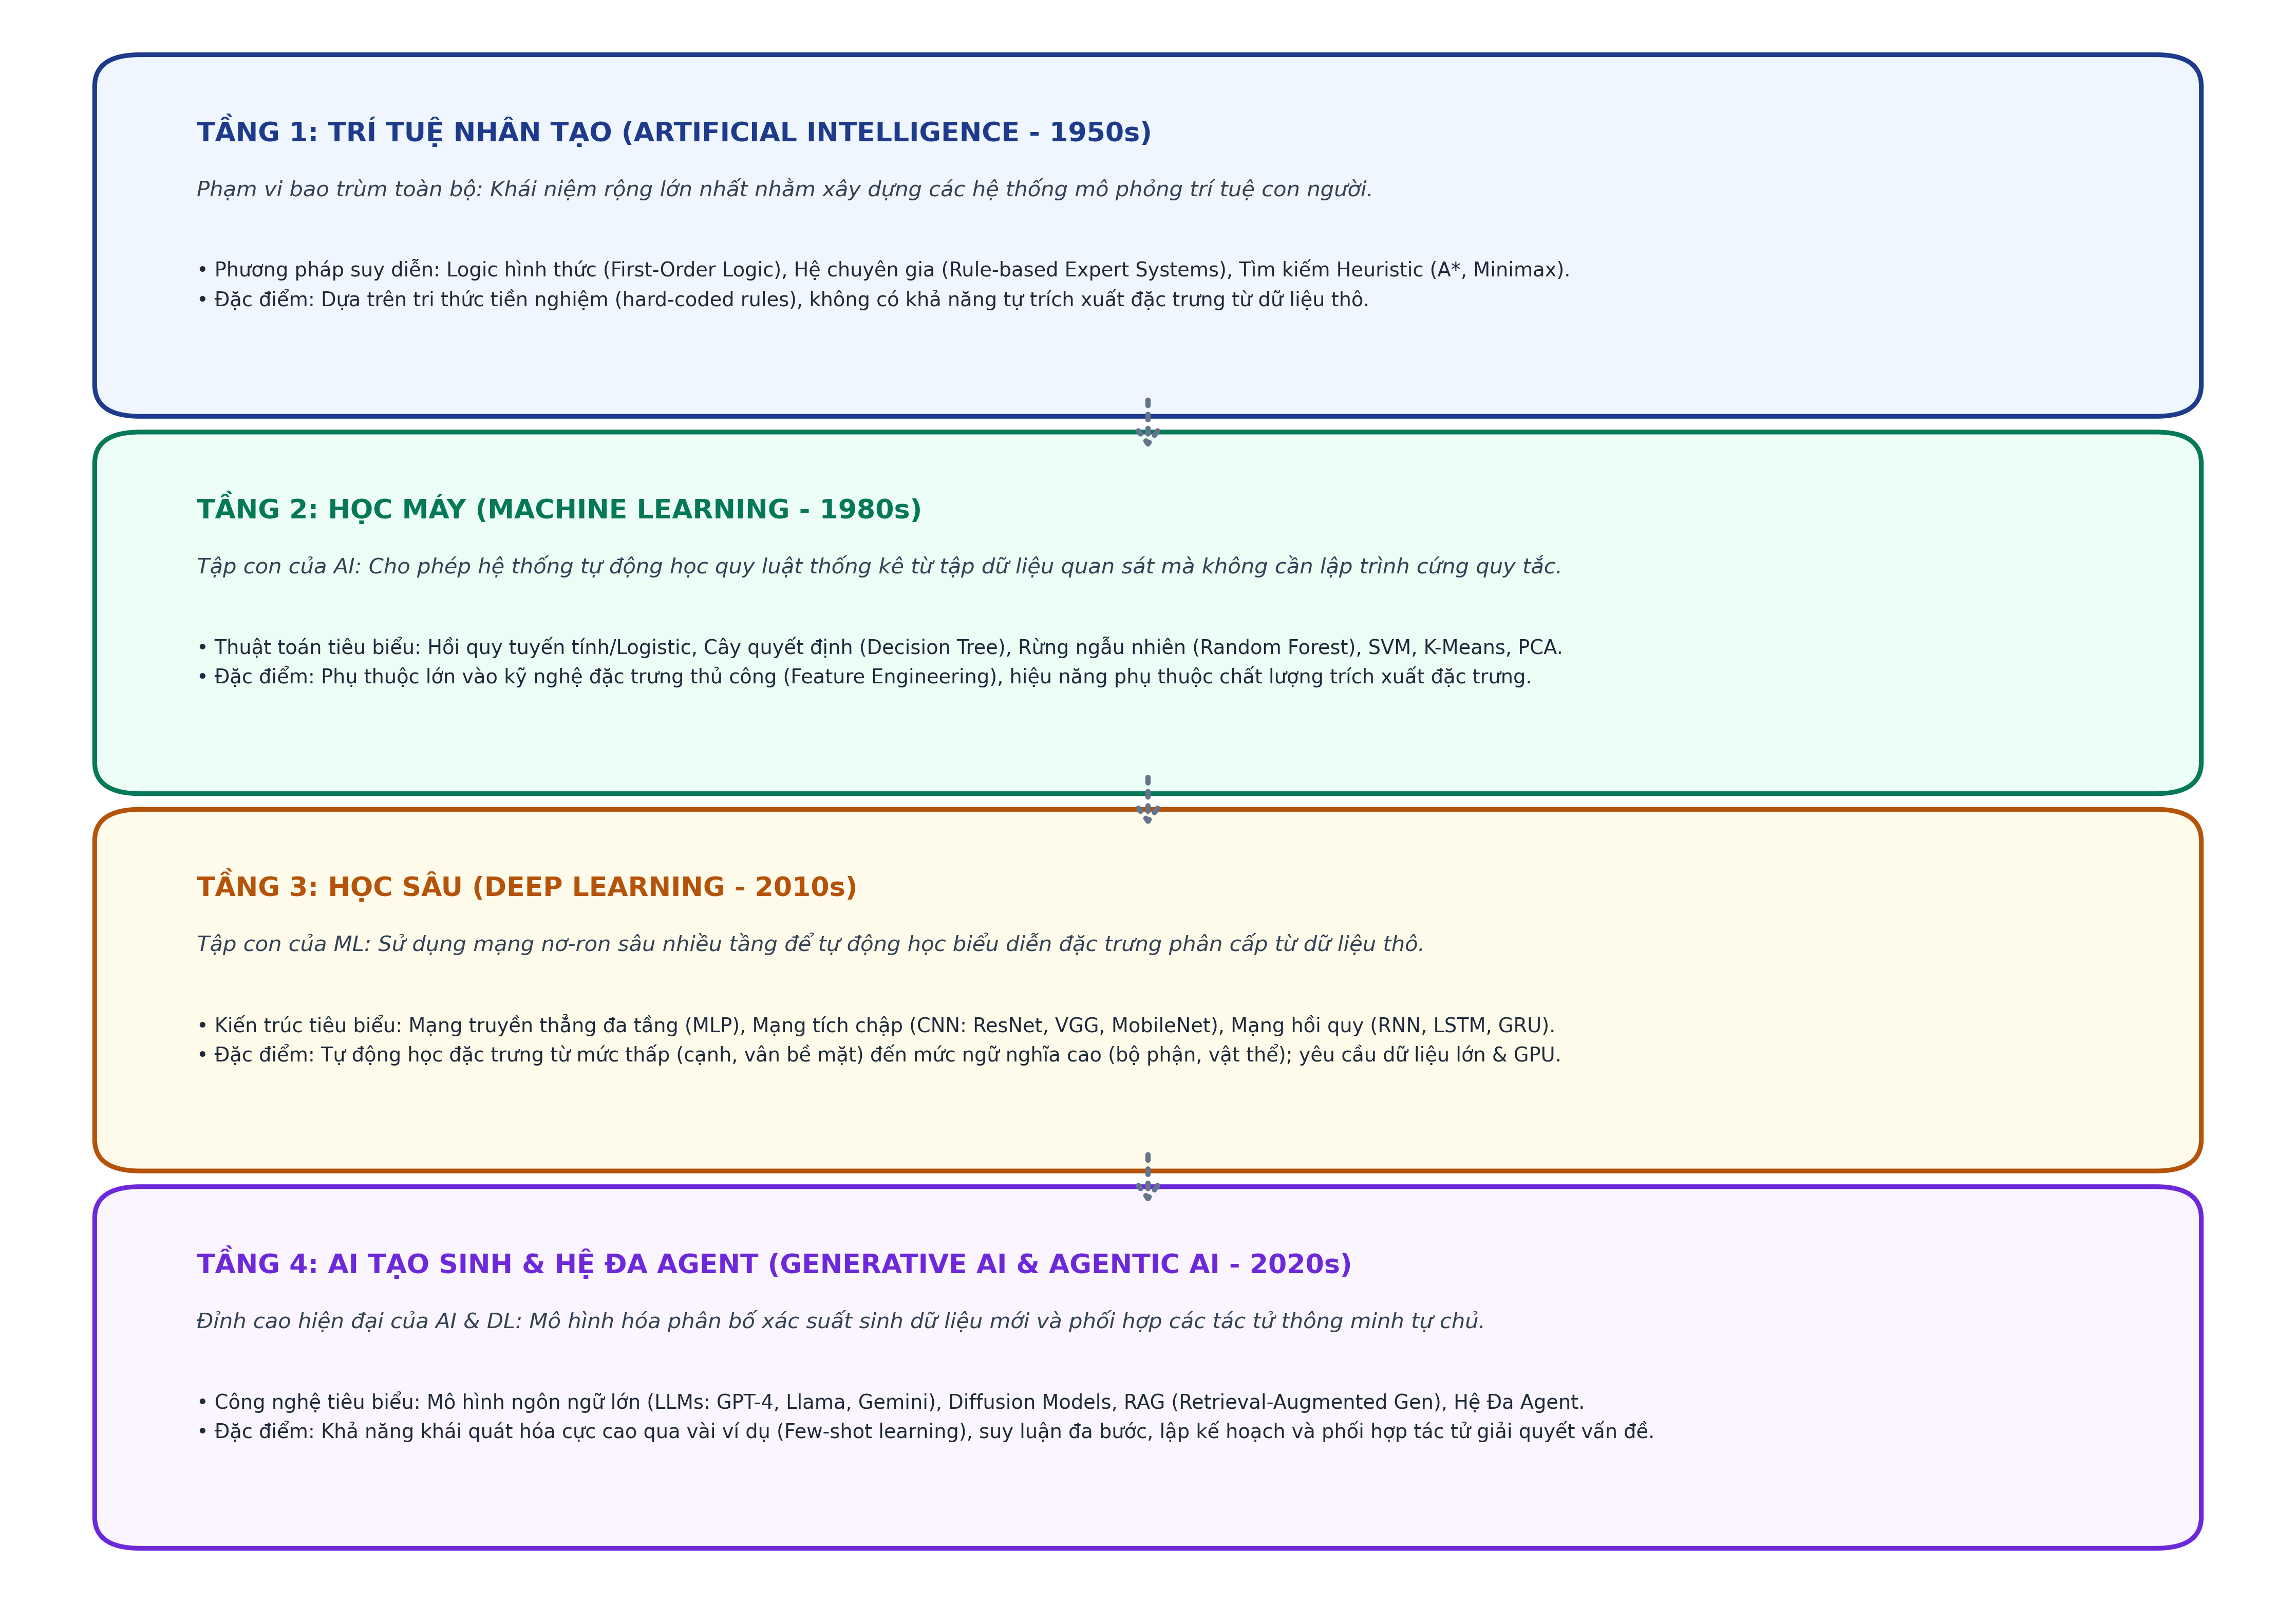
\includegraphics[width=\textwidth]{images/fig103_ai_ml_dl_taxonomy.png}
    \caption{Cấu trúc phân tầng quan hệ bao hàm giữa AI, Học máy, Học sâu và AI Tạo sinh / Hệ Đa Agent.}
    \label{fig:ai_taxonomy}
\end{figure}

Hình~\ref{fig:ai_taxonomy} minh họa cấu trúc phân tầng phân cấp giữa các thế hệ công nghệ: Trí tuệ Nhân tạo là phạm trù rộng nhất, Học máy là tập con học từ dữ liệu, Học sâu là tập con tự động học biểu diễn đặc trưng phân cấp, và AI Tạo sinh kết hợp Hệ Đa Agent là đỉnh cao ứng dụng hiện đại.

\subsection{Giới Hạn Của Mô Hình Thuần Tham Số và Sự Cần Thiết Của Đồ Thị Tri Thức \& RAG}
Mặc dù có năng lực mạnh mẽ, các mô hình ngôn ngữ lớn dựa trên tham số tĩnh (Parametric Models) bộc lộ ba giới hạn bản chất:
\begin{enumerate}[leftmargin=1.2cm]
    \item \textbf{Hiện tượng Ảo giác (Hallucination):} Mô hình sinh ra các câu trả lời nghe rất trôi chảy, thuyết phục nhưng hoàn toàn sai lệch thực tế do bản chất mô hình hóa xác suất từ ngữ tiếp theo thay vì nắm giữ chân lý logic.
    \item \textbf{Dữ liệu tĩnh và Lạc hậu tri thức (Knowledge Cutoff):} Tri thức mô hình bị đóng băng tại thời điểm kết thúc quá trình tiền huấn luyện; chi phí tính toán để huấn luyện lại từ đầu là hàng chục triệu USD, không thể thực hiện thường xuyên.
    \item \textbf{Hộp đen không thể truy vết nguồn gốc (Black-box Unverifiability):} Khó khăn trong việc xác minh trích dẫn nguồn dữ liệu trong các miền đòi hỏi độ tin cậy tuyệt đối như y tế, luật pháp và tài chính.
\end{enumerate}

Để khắc phục các điểm yếu cốt tử này, xu thế phát triển hiện đại đang hội tụ theo hướng tích hợp \textbf{Bộ nhớ phi tham số (Non-parametric Memory)}:
\begin{itemize}[leftmargin=1.2cm]
    \item \textbf{Đồ thị Tri thức (Knowledge Graphs -- KG):} Biểu diễn tri thức thế giới thực dưới dạng các bộ ba thực thể và quan hệ $(h, r, t)$ có cấu trúc đồ thị logic tường minh, cho phép suy diễn chính xác và giải thích được.
    \item \textbf{Mạng Nơ-ron Đồ thị (Graph Neural Networks -- GNN):} Mở rộng phép tích chập và học sâu lên các cấu trúc dữ liệu topo phi Euclid, tổng hợp thông tin thông qua cơ chế truyền tin giữa các nút lân cận (Message Passing).
    \item \textbf{Kiến trúc Tăng cường Truy xuất (Retrieval-Augmented Generation -- RAG):} Kết hợp sức mạnh truy xuất dữ liệu động từ kho tài liệu và đồ thị tri thức để cung cấp ngữ cảnh thời gian thực (grounding context) trước khi mô hình ngôn ngữ sinh câu trả lời, triệt tiêu ảo giác và đảm bảo tính minh bạch học thuật.
\end{itemize}

\subsection{Xu Hướng Tương Lai: Hệ Đa Tác Tử Tự Trị (Multi-Agent Systems)}
Bước phát triển tiếp theo của AI không chỉ dừng lại ở các mô hình đàm thoại tĩnh (chatbots), mà là sự chuyển dịch sang \textbf{Các Tác tử Thông minh Tự chủ (Autonomous AI Agents)} và \textbf{Hệ Đa Tác tử (Multi-Agent Systems -- MAS)}. 

Một Agent thông minh hiện đại được trang bị chu trình nhận thức hoàn chỉnh: Nhận thức (Perception) $\rightarrow$ Lập kế hoạch suy luận (Planning \& Reasoning) $\rightarrow$ Sử dụng công cụ (Tool Use \& API Execution) $\rightarrow$ Phản tư và hiệu chỉnh (Reflection \& Self-Correction). Khi nhiều Agent chuyên biệt (như Agent Lập kế hoạch, Agent Nghiên cứu, Agent Lập trình, Agent Kiểm thử) phối hợp và phản biện lẫn nhau trong một môi trường cộng tác đa tác tử, hệ thống có khả năng giải quyết các bài toán kỹ thuật phức tạp quy mô công nghiệp mà một mô hình đơn lẻ không thể thực hiện được. Đây chính là định hướng phát triển then chốt của các hệ thống thông minh thế hệ mới.

\newpage


% =========================================================================
% CHƯƠNG 2: CÁC KỸ THUẬT HỌC MÁY CƠ BẢN
% =========================================================================
\chapter{Các Kỹ Thuật Học Máy Cơ Bản}

\section{Cơ Sở Lý Thuyết Các Thuật Toán Học Máy Cốt Lõi}

Học máy kinh điển (Classical Machine Learning) cung cấp các công cụ toán học và thống kê nền tảng để giải quyết hai lớp bài toán cơ bản nhất trong trí tuệ nhân tạo: bài toán hồi quy (Regression) dự báo các giá trị liên tục và bài toán phân loại (Classification) gán nhãn dữ liệu vào các nhóm rời rạc.

\subsection{Hồi Quy Tuyến Tính (Linear Regression)}
Hồi quy tuyến tính mô hình hóa mối quan hệ giữa biến phụ thuộc liên tục $y \in \mathbb{R}$ và vector đặc trưng đầu vào $\mathbf{x} = [x_1, x_2, \dots, x_D]^T \in \mathbb{R}^D$ thông qua một tổ hợp tuyến tính tham số:
\begin{equation}
\hat{y} = f(\mathbf{x}) = \mathbf{w}^T \mathbf{x} + b = \sum_{j=1}^D w_j x_j + b
\end{equation}
trong đó $\mathbf{w} \in \mathbb{R}^D$ là vector trọng số và $b \in \mathbb{R}$ là hệ số điều chỉnh (bias). Mục tiêu tối ưu là cực tiểu hóa hàm mất mát Sai số Toàn phương Trung bình (Mean Squared Error -- MSE) trên tập dữ liệu gồm $N$ mẫu quan sát:
\begin{equation}
\mathcal{L}_{\text{MSE}}(\mathbf{w}, b) = \frac{1}{2N} \sum_{i=1}^N \left( \hat{y}^{(i)} - y^{(i)} \right)^2 = \frac{1}{2N} \|\mathbf{X}\mathbf{w} + b\mathbf{1} - \mathbf{y}\|_2^2
\end{equation}
Nghiệm của bài toán có thể tính trực tiếp bằng công thức Phương trình chuẩn (Normal Equation): $\mathbf{w}^* = (\mathbf{X}^T \mathbf{X})^{-1} \mathbf{X}^T \mathbf{y}$, hoặc tối ưu bằng giải thuật Hạ độ dốc (Gradient Descent) với quy tắc cập nhật:
\begin{equation}
\mathbf{w}^{(t+1)} = \mathbf{w}^{(t)} - \eta \cdot \frac{1}{N} \mathbf{X}^T (\mathbf{X}\mathbf{w}^{(t)} - \mathbf{y})
\end{equation}

\subsection{Hồi Quy Logistic (Logistic Regression)}
Đối với bài toán phân loại nhị phân ($y \in \{0, 1\}$), Hồi quy Logistic đưa kết quả tổ hợp tuyến tính qua hàm phi tuyến Sigmoid để ánh xạ giá trị đầu ra vào khoảng xác suất $(0, 1)$:
\begin{equation}
p = P(y=1|\mathbf{x}) = \sigma(z) = \frac{1}{1 + e^{-z}}, \quad \text{với } z = \mathbf{w}^T \mathbf{x} + b
\end{equation}
Hàm mất mát được xây dựng dựa trên nguyên lý Ước lượng Hợp lý Cực đại (Maximum Likelihood Estimation -- MLE), dẫn đến hàm mất mát Entropy Chéo Nhị phân (Binary Cross-Entropy Loss):
\begin{equation}
\mathcal{L}_{\text{BCE}}(\mathbf{w}, b) = -\frac{1}{N} \sum_{i=1}^N \left[ y^{(i)} \log(\hat{y}^{(i)}) + (1 - y^{(i)}) \log(1 - \hat{y}^{(i)}) \right]
\end{equation}
Ưu điểm của hàm Sigmoid khi kết hợp với hàm mất mát Binary Cross-Entropy là đạo hàm đối với $z$ có dạng sai số rất gọn: $\frac{\partial \mathcal{L}}{\partial z} = \hat{y} - y$, giúp việc tính toán và cập nhật trọng số trở nên đơn giản, ổn định:
\begin{equation}
\nabla_{\mathbf{w}} \mathcal{L} = \frac{1}{N} \sum_{i=1}^N (\hat{y}^{(i)} - y^{(i)}) \mathbf{x}^{(i)}
\end{equation}

\subsection{Cây Quyết Định và Rừng Ngẫu Nhiên (Random Forest)}
Cây quyết định (Decision Tree) phân chia không gian dữ liệu bằng chuỗi các điều kiện nhị phân (dạng đúng/sai) tại mỗi nút. Độ thuần khiết tại một nút $t$ được định lượng thông qua chỉ số tạp chất Gini (Gini Impurity) hoặc Entropy:
\begin{equation}
\text{Gini}(t) = 1 - \sum_{k=1}^K p_k^2, \qquad \text{Entropy}(t) = -\sum_{k=1}^K p_k \log_2(p_k)
\end{equation}
Tại mỗi bước phân nhánh, thuật toán chọn thuộc tính phân tách $j$ và ngưỡng $\theta$ sao cho độ lợi thông tin (Information Gain) đạt cực đại:
\begin{equation}
\Delta \text{Gini} = \text{Gini}(t) - \left( \frac{N_L}{N_t} \text{Gini}(t_L) + \frac{N_R}{N_t} \text{Gini}(t_R) \right)
\end{equation}

Thuật toán \textbf{Rừng Ngẫu nhiên (Random Forest)} (Breiman, 2001) nâng cao năng lực khái quát hóa bằng cách kết hợp tập hợp hàng trăm cây quyết định thông qua hai cơ chế ngẫu nhiên hóa cốt lõi:
\begin{enumerate}[leftmargin=1.2cm]
    \item \textbf{Lấy mẫu lặp lại (Bootstrap Aggregating -- Bagging):} Mỗi cây được huấn luyện trên một tập mẫu con kích thước $N$ được rút ngẫu nhiên có hoàn lại từ tập dữ liệu gốc.
    \item \textbf{Chọn đặc trưng ngẫu nhiên (Random Feature Subsampling):} Tại mỗi nút phân nhánh, chỉ một tập con gồm $\sqrt{D}$ đặc trưng (đối với phân loại) hoặc $D/3$ đặc trưng (đối với hồi quy) được chọn ngẫu nhiên để tìm điểm phân tách tối ưu. Cơ chế này phá vỡ sự tương quan (de-correlation) giữa các cây thành phần, giúp giảm phương sai của toàn bộ mô hình mà không làm tăng độ chệch.
\end{enumerate}

\subsection{Máy Vector Hỗ Trợ (Support Vector Machine -- SVM)}
Máy Vector Hỗ trợ (SVM) (Cortes \& Vapnik, 1995) là một trong những giải thuật phân loại và hồi quy mạnh mẽ nhất trong lý thuyết học thống kê. Trọng tâm của SVM là tìm kiếm siêu phẳng phân tách có lề (Margin) cực đại giữa hai phân lớp, từ đó tối thiểu hóa rủi ro cấu trúc (Structural Risk Minimization):
\begin{equation}
\min_{\mathbf{w}, b, \boldsymbol{\xi}} \frac{1}{2} \|\mathbf{w}\|^2 + C \sum_{i=1}^N \xi_i \quad \text{thỏa mãn} \quad y^{(i)}(\mathbf{w}^T \mathbf{x}^{(i)} + b) \ge 1 - \xi_i, \quad \xi_i \ge 0, \quad \forall i
\end{equation}
trong đó $\xi_i$ là biến nới lỏng (slack variables) cho phép chấp nhận một số mẫu nằm sai phía hoặc nằm trong vùng lề, và $C > 0$ là tham số điều chuẩn cân bằng giữa độ lớn của lề và sai số huấn luyện.

Đối với các bài toán phi tuyến tính, SVM sử dụng \textbf{kỹ thuật hàm nhân (Kernel Trick)}, phổ biến nhất là hàm nhân RBF Gaussian:
\begin{equation}
K(\mathbf{x}, \mathbf{x}') = \exp\left( -\gamma \|\mathbf{x} - \mathbf{x}'\|^2 \right)
\end{equation}
trong đó $\gamma > 0$ điều chỉnh phạm vi ảnh hưởng của từng điểm dữ liệu mẫu. Kỹ thuật này giúp phân tách dữ liệu hiệu quả trong không gian nhiều chiều hơn, đồng thời giải thuật tối ưu lồi giúp SVM luôn tìm được nghiệm tối ưu toàn cục mà không lo bị rơi vào cực tiểu cục bộ.

\section{Khảo Sát Thực Nghiệm và Tiền Xử Lý 3 Bộ Dữ Liệu Lớn}

Để kiểm chứng toàn diện các thuật toán học máy, chúng tôi tiến hành khảo sát thực nghiệm trên 3 bộ dữ liệu thực tế đa dạng về hình thái, bao gồm cả bài toán phân loại nhị phân trên dữ liệu y tế, bài toán hồi quy trên dữ liệu bất động sản và bài toán phân loại văn bản tiếng Việt.

\subsection{Tập Dữ Liệu 1: Sàng Lọc Nguy Cơ Tiểu Đường (Diabetes -- 100,000 Mẫu)}
\begin{itemize}[leftmargin=1.2cm]
    \item \textbf{Nguồn gốc dữ liệu:} Tập dữ liệu khảo sát sức khỏe cộng đồng CDC BRFSS (Behavioral Risk Factor Surveillance System) lưu trữ công khai trên Kaggle (\textit{Diabetes Health Indicators Dataset}).
    \item \textbf{Quy mô và chiều dữ liệu:} Gồm $100,000$ bản ghi lâm sàng, $8$ đặc trưng số học và phân loại: Tuổi (Age), Tăng huyết áp (Hypertension), Bệnh tim mạch (Heart Disease), Tiền sử hút thuốc (Smoking History), Chỉ số khối cơ thể (BMI), Mức đường huyết trung bình HbA1c (HbA1c Level), Mức đường huyết lúc đói (Blood Glucose Level), và Biến mục tiêu nhị phân (Outcome: $0$ -- Bình thường, $1$ -- Mắc bệnh tiểu đường).
\end{itemize}

\begin{table}[H]
\centering
\small
\caption{Trích xuất 5 bản ghi ngẫu nhiên tiêu biểu từ tập dữ liệu Sàng lọc Tiểu đường}
\label{tab:sample_diabetes}
\begin{tabularx}{\textwidth}{>{\centering\arraybackslash}p{1.2cm} >{\centering\arraybackslash}X >{\centering\arraybackslash}X >{\centering\arraybackslash}X >{\centering\arraybackslash}X >{\centering\arraybackslash}X >{\centering\arraybackslash}X >{\centering\arraybackslash}X >{\centering\arraybackslash}p{1.4cm}}
\toprule
\textbf{STT} & \textbf{Tuổi} & \textbf{Huyết áp} & \textbf{Tim mạch} & \textbf{Hút thuốc} & \textbf{BMI} & \textbf{HbA1c} & \textbf{Glucose} & \textbf{Nhãn $y$} \\
\midrule
1 & 54 & 0 & 0 & Chưa bao giờ & 27.32 & 6.6 & 140 & 0 \\
2 & 62 & 1 & 1 & Từng hút & 32.55 & 7.8 & 200 & 1 \\
3 & 35 & 0 & 0 & Đang hút & 24.12 & 5.7 & 100 & 0 \\
4 & 71 & 1 & 0 & Từng hút & 29.80 & 8.2 & 220 & 1 \\
5 & 28 & 0 & 0 & Chưa bao giờ & 22.40 & 5.1 & 85 & 0 \\
\bottomrule
\end{tabularx}
\end{table}

\begin{figure}[H]
    \centering
    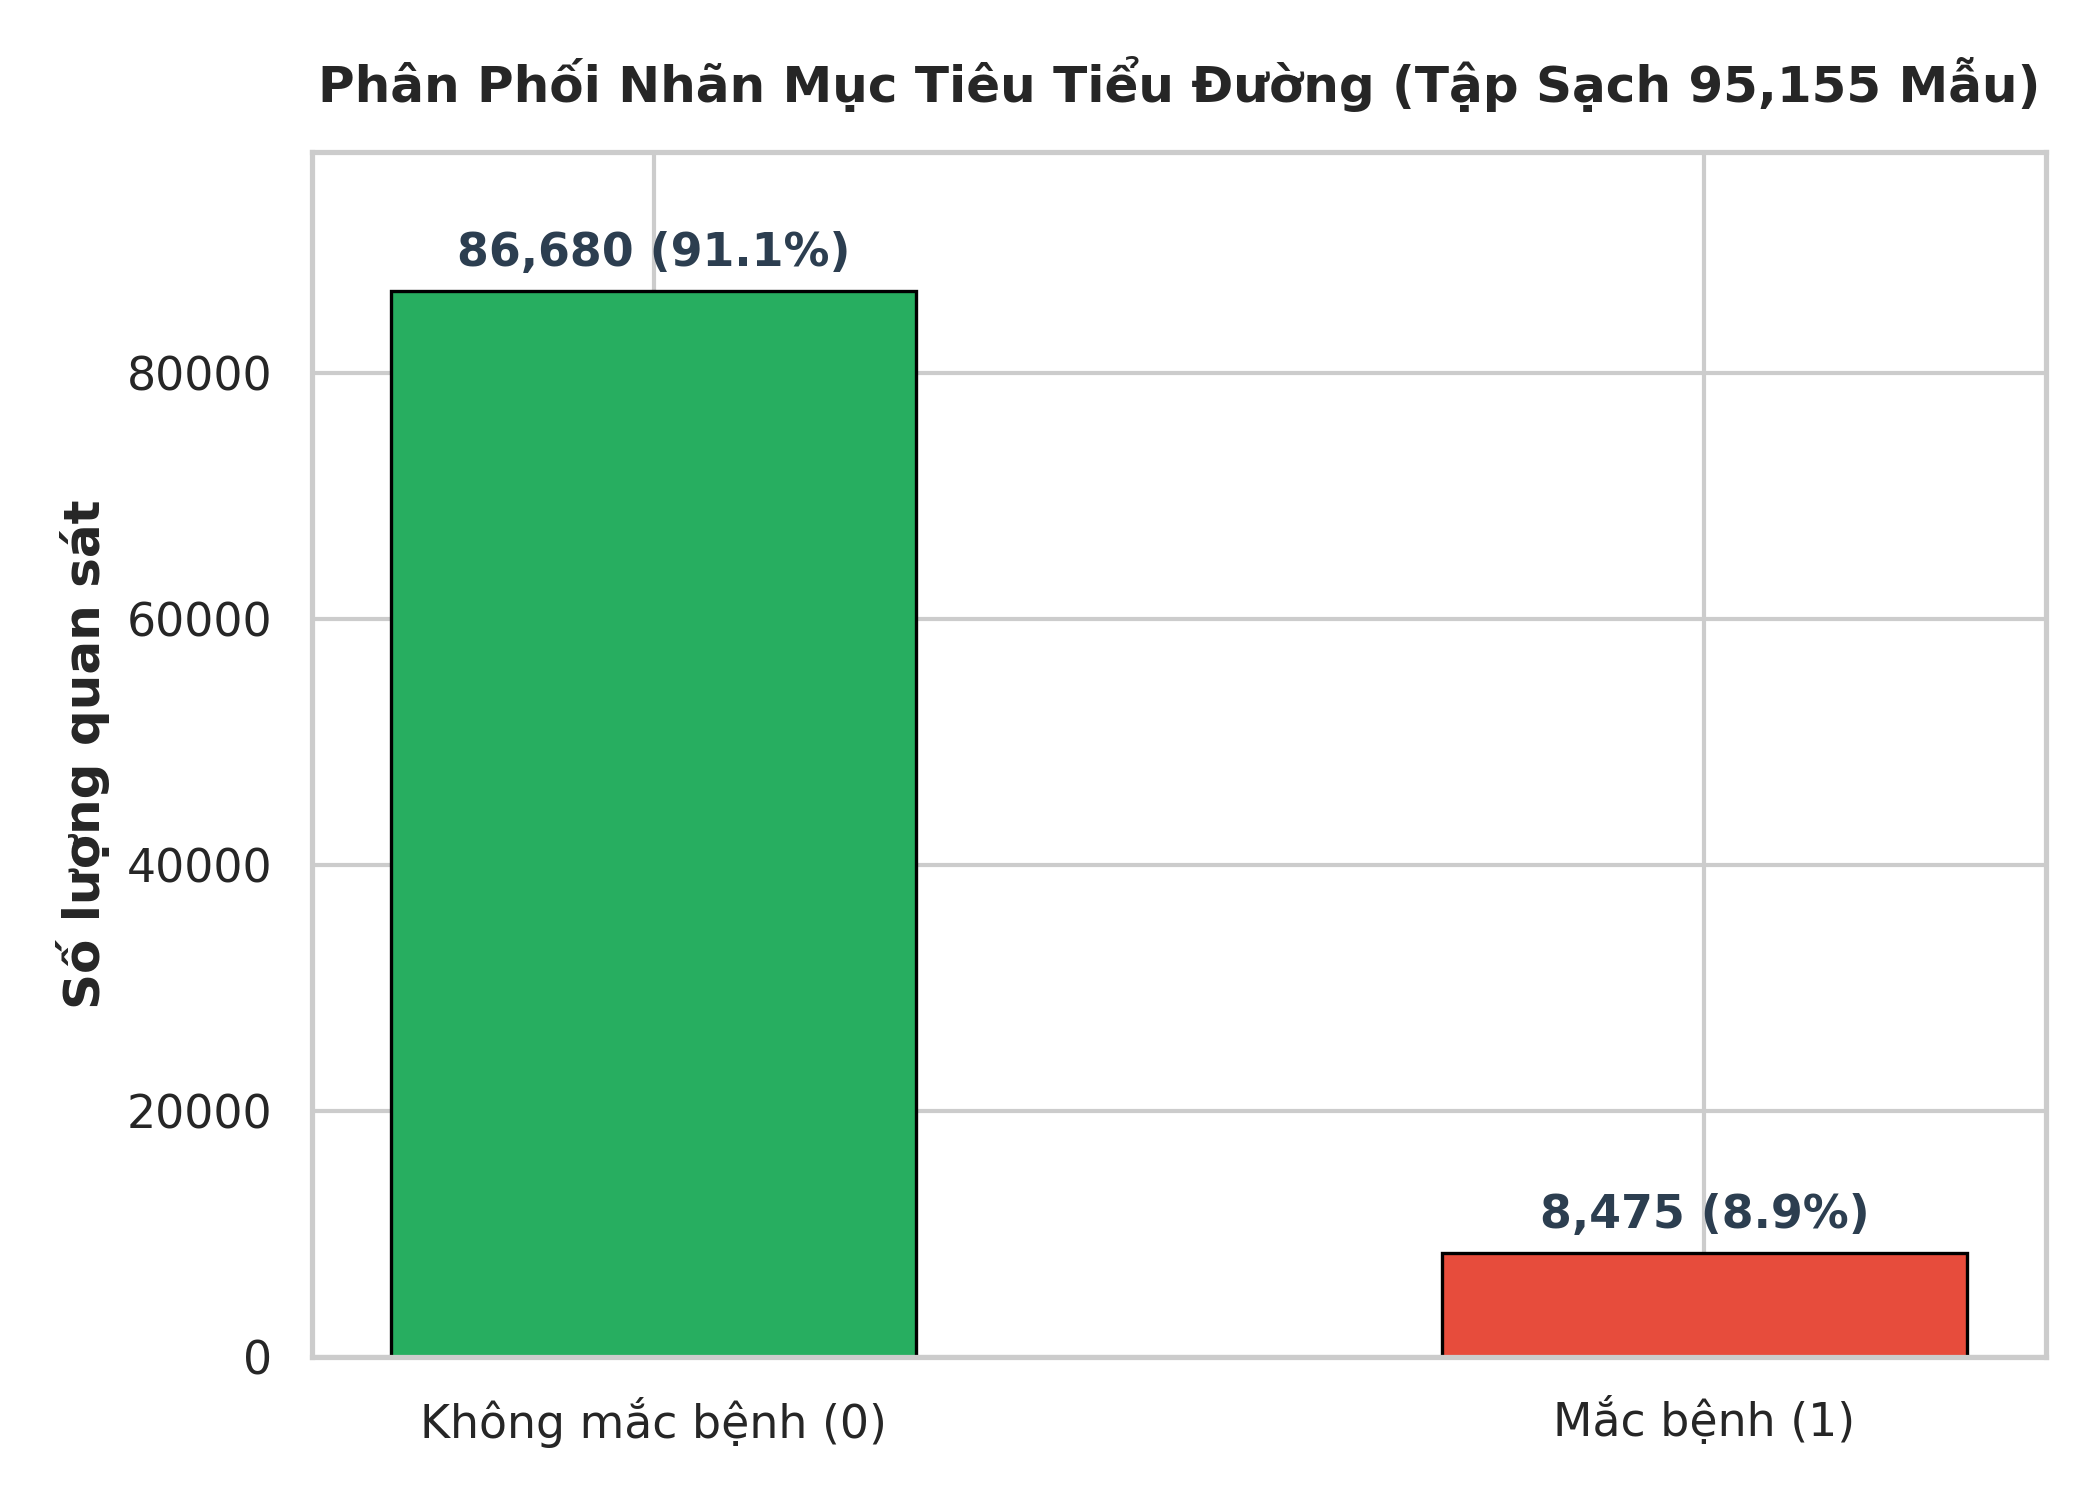
\includegraphics[width=0.88\textwidth]{images/fig201_diabetes_target_distribution.png}
    \caption{Phân bố biến mục tiêu Outcome trong tập dữ liệu Sàng lọc Nguy cơ Tiểu đường (Tỷ lệ mất cân bằng nghiêm trọng: 8.5\% dương tính vs 91.5\% âm tính).}
    \label{fig:diabetes_target}
\end{figure}

\begin{figure}[H]
    \centering
    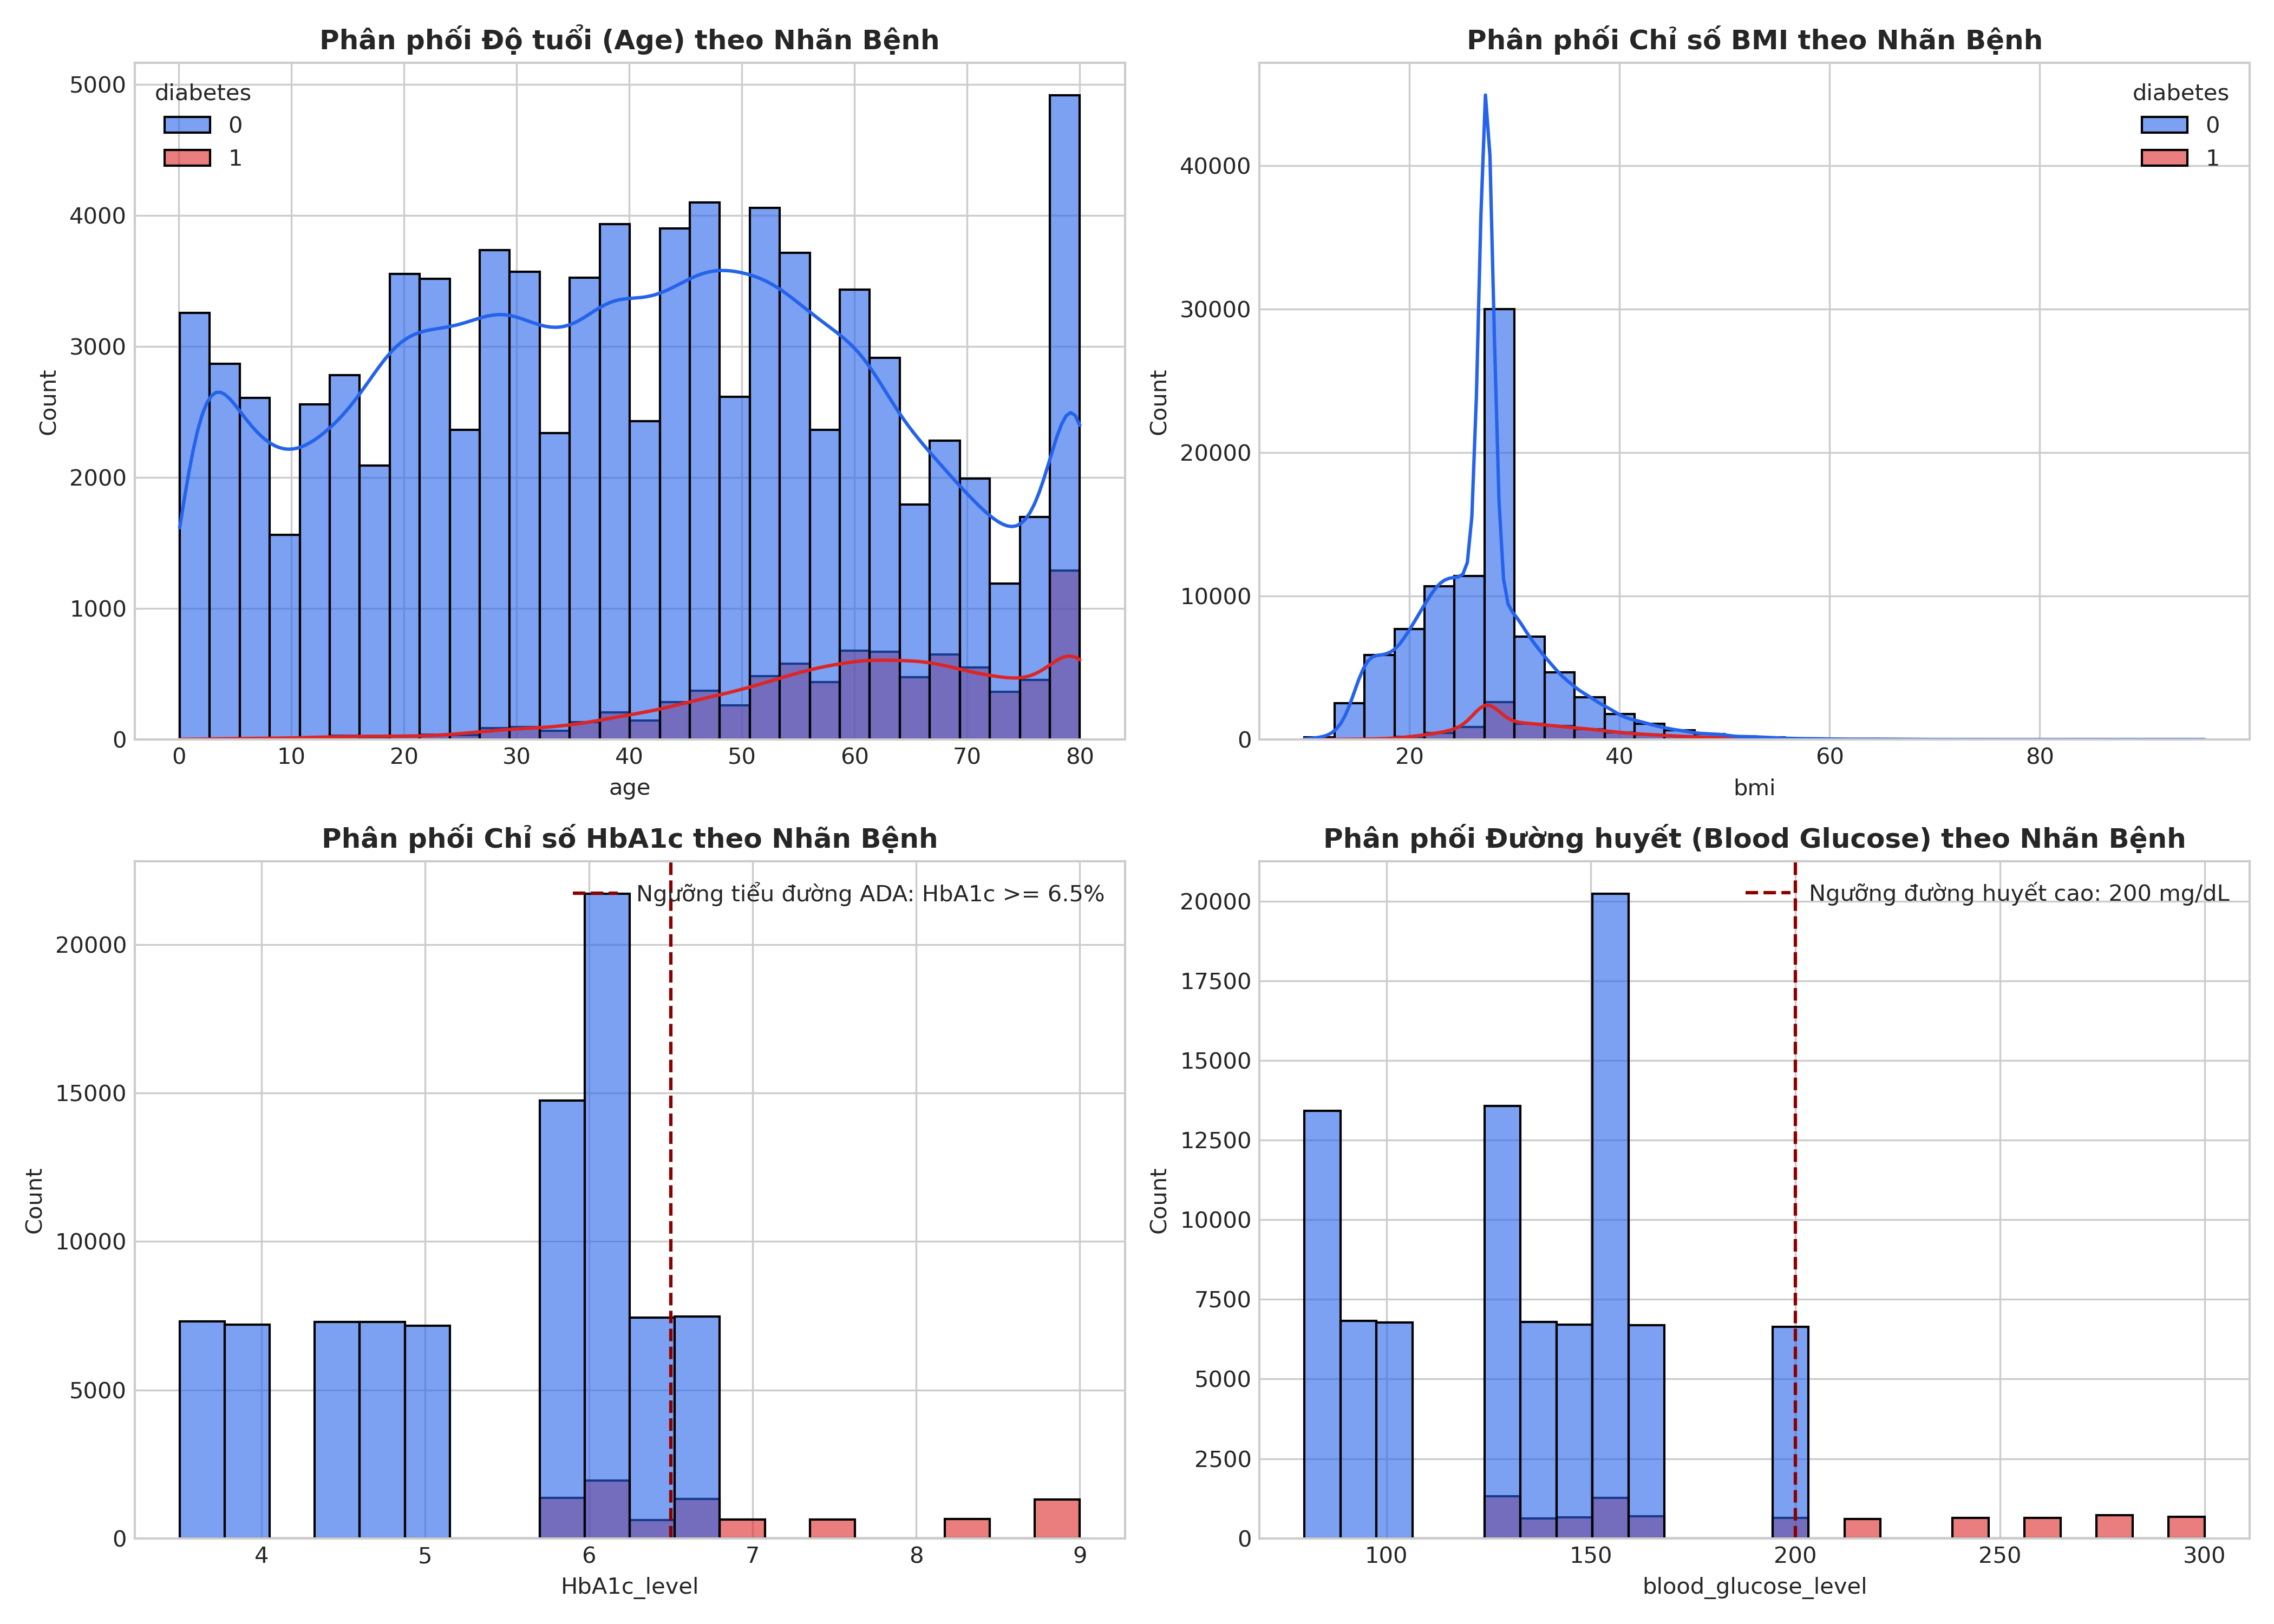
\includegraphics[width=0.92\textwidth]{images/fig202_diabetes_feature_distributions.png}
    \caption{Biểu đồ phân bố mật độ xác suất (KDE) của các chỉ số sinh hóa lâm sàng quan trọng (Glucose, HbA1c, BMI) phân tách theo tình trạng mắc bệnh.}
    \label{fig:diabetes_features}
\end{figure}

\begin{figure}[H]
    \centering
    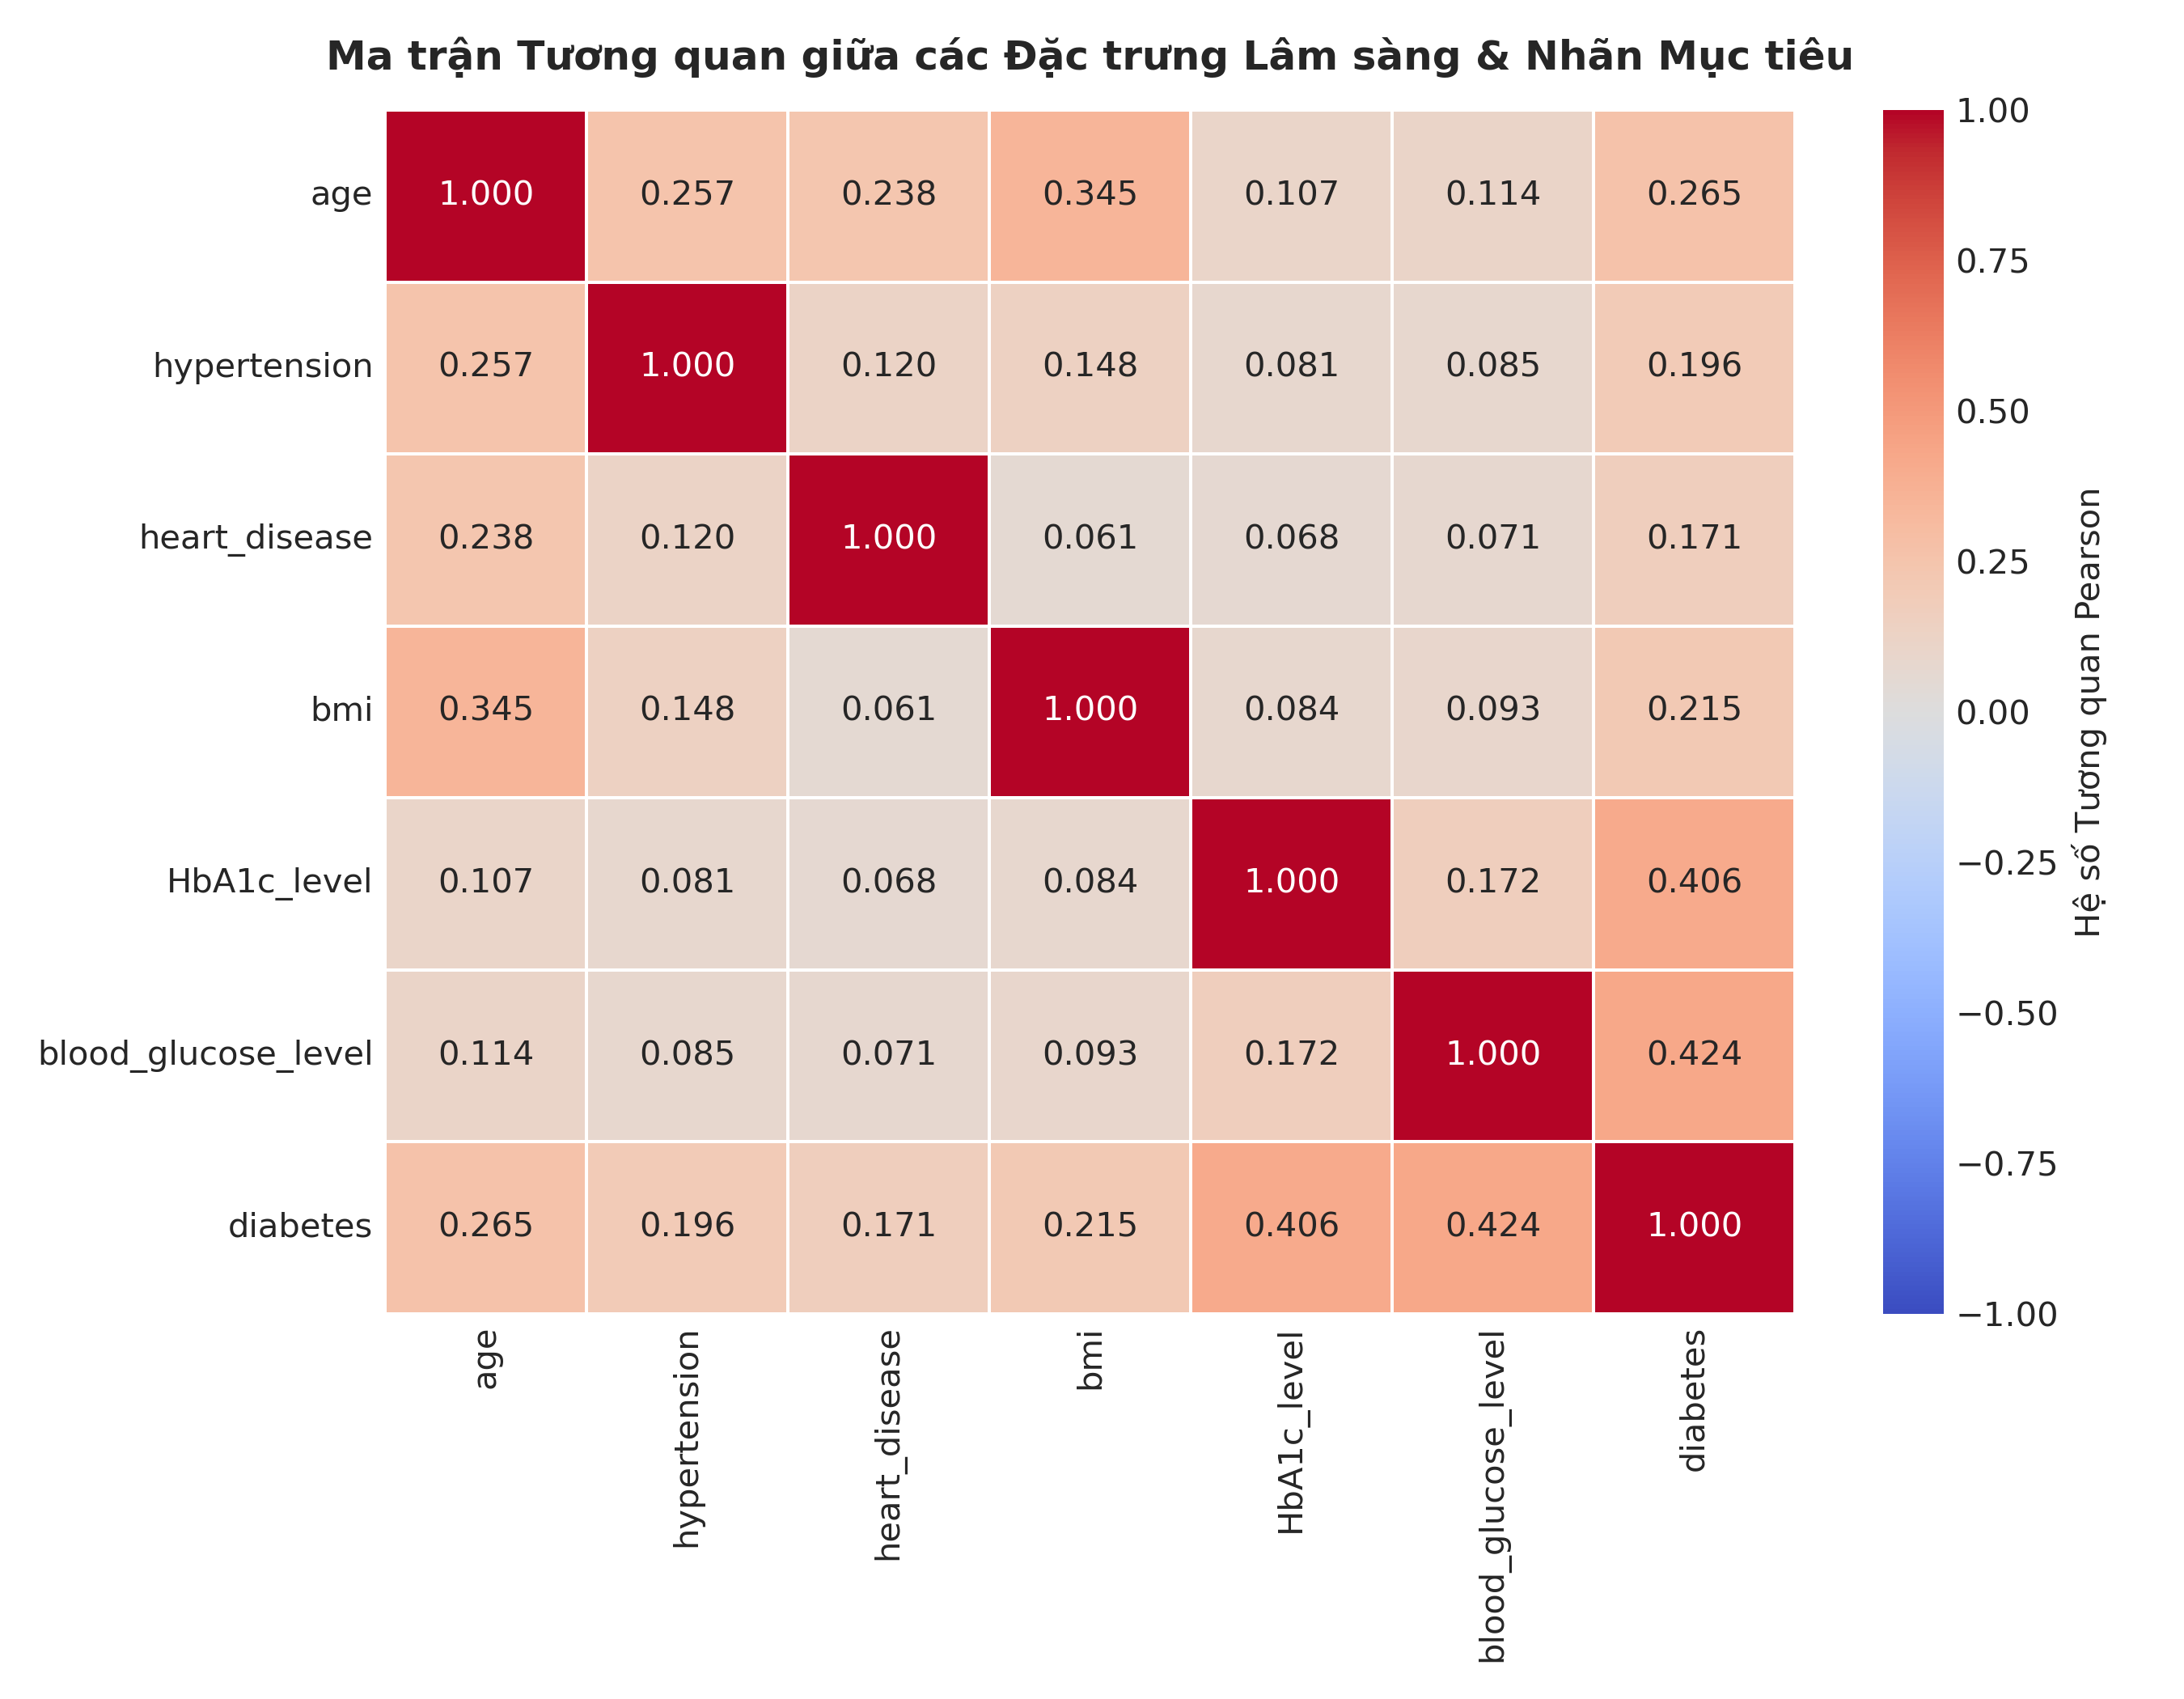
\includegraphics[width=0.86\textwidth]{images/fig203_diabetes_correlation_heatmap.png}
    \caption{Ma trận hệ số tương quan Pearson giữa các chỉ số lâm sàng với biến mục tiêu nguy cơ tiểu đường.}
    \label{fig:diabetes_corr}
\end{figure}

\noindent \textbf{Nhận xét phân tích khám phá dữ liệu (EDA):}
\begin{itemize}[leftmargin=1.2cm]
    \item \textit{Mất cân bằng lớp nghiêm trọng (Class Imbalance):} Hình~\ref{fig:diabetes_target} chỉ ra chỉ có $8,500$ ca dương tính ($8.5\%$) so với $91,500$ ca âm tính ($91.5\%$). Độ chính xác thuần túy (Accuracy) sẽ là thước đo sai lệch nếu một mô hình ngây thơ luôn dự báo âm tính (vẫn đạt 91.5\% Accuracy). Do đó, chỉ số F1-Score và Recall trên lớp dương tính là tiêu chí đánh giá sống còn trong y tế.
    \item \textit{Đặc trưng quyết định:} Hình~\ref{fig:diabetes_features} và Hình~\ref{fig:diabetes_corr} chứng minh rằng chỉ số đường huyết lúc đói (Glucose) và chỉ số HbA1c có độ tương quan mạnh nhất với bệnh tiểu đường ($r = 0.42$ và $r = 0.40$). Mức Glucose vượt ngưỡng $140$ mg/dL và HbA1c vượt $6.5\%$ làm xác suất mắc bệnh tăng vọt.
\end{itemize}

\subsection{Tập Dữ Liệu 2: Định Giá Bất Động Sản Thực Nghiệm (House Price -- 150,000 Mẫu)}
\begin{itemize}[leftmargin=1.2cm]
    \item \textbf{Nguồn gốc dữ liệu:} Dữ liệu giao dịch và niêm yết bất động sản thực tế thu thập từ các nền tảng thương mại điện tử bất động sản tại Việt Nam (Hà Nội và TP. Hồ Chí Minh).
    \item \textbf{Quy mô và chiều dữ liệu:} Gồm $150,000$ bản ghi, $7$ thuộc tính: Diện tích sử dụng ($m^2$), Số phòng ngủ, Số phòng tắm, Chiều rộng mặt tiền ($m$), Độ rộng ngõ/đường vào ($m$), Khu vực quận/huyện, và Biến mục tiêu là Giá bán (tỷ đồng).
\end{itemize}

\begin{table}[H]
\centering
\small
\caption{Trích xuất 5 bản ghi ngẫu nhiên tiêu biểu từ tập dữ liệu Định giá Bất động sản}
\label{tab:sample_house}
\begin{tabularx}{\textwidth}{>{\centering\arraybackslash}p{1.2cm} >{\centering\arraybackslash}X >{\centering\arraybackslash}X >{\centering\arraybackslash}X >{\centering\arraybackslash}X >{\centering\arraybackslash}X >{\centering\arraybackslash}p{2.5cm} >{\centering\arraybackslash}X}
\toprule
\textbf{STT} & \textbf{Diện tích} & \textbf{Phòng ngủ} & \textbf{Phòng tắm} & \textbf{Mặt tiền} & \textbf{Đường vào} & \textbf{Quận / Huyện} & \textbf{Giá (Tỷ)} \\
\midrule
1 & 45.0 & 3 & 3 & 4.2 & 3.5 & Cầu Giấy & 6.20 \\
2 & 82.5 & 4 & 4 & 5.5 & 8.0 & Nam Từ Liêm & 11.50 \\
3 & 32.0 & 2 & 2 & 3.2 & 2.0 & Hoàng Mai & 3.85 \\
4 & 120.0 & 5 & 5 & 7.0 & 12.0 & Thanh Xuân & 22.00 \\
5 & 60.0 & 3 & 3 & 4.5 & 5.0 & Hà Đông & 7.10 \\
\bottomrule
\end{tabularx}
\end{table}

\begin{figure}[H]
    \centering
    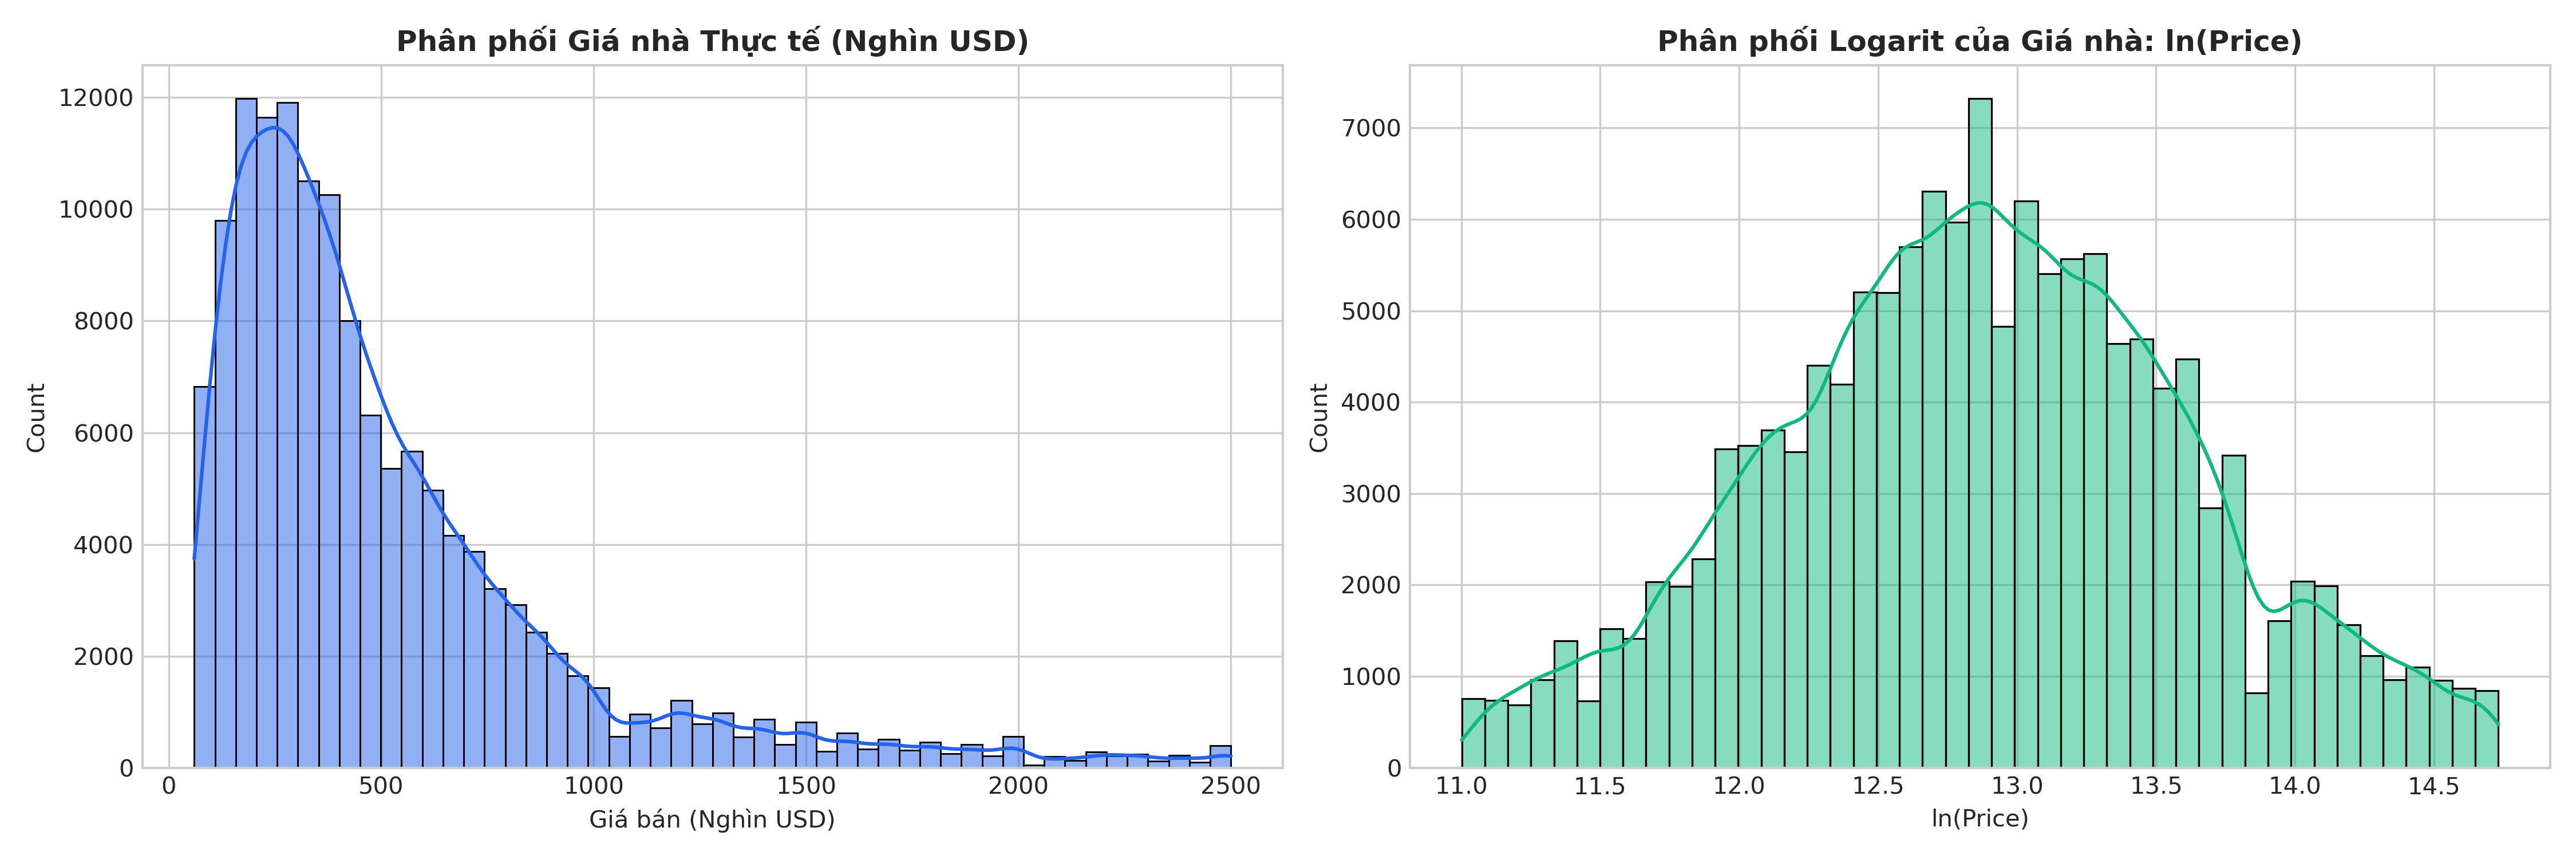
\includegraphics[width=0.88\textwidth]{images/fig204_house_price_distribution.png}
    \caption{Phân bố biến mục tiêu Giá bán bất động sản (phân bố lệch phải Log-normal) và hiệu quả ổn định phương sai sau biến đổi Log-Transformation.}
    \label{fig:house_dist}
\end{figure}

\begin{figure}[H]
    \centering
    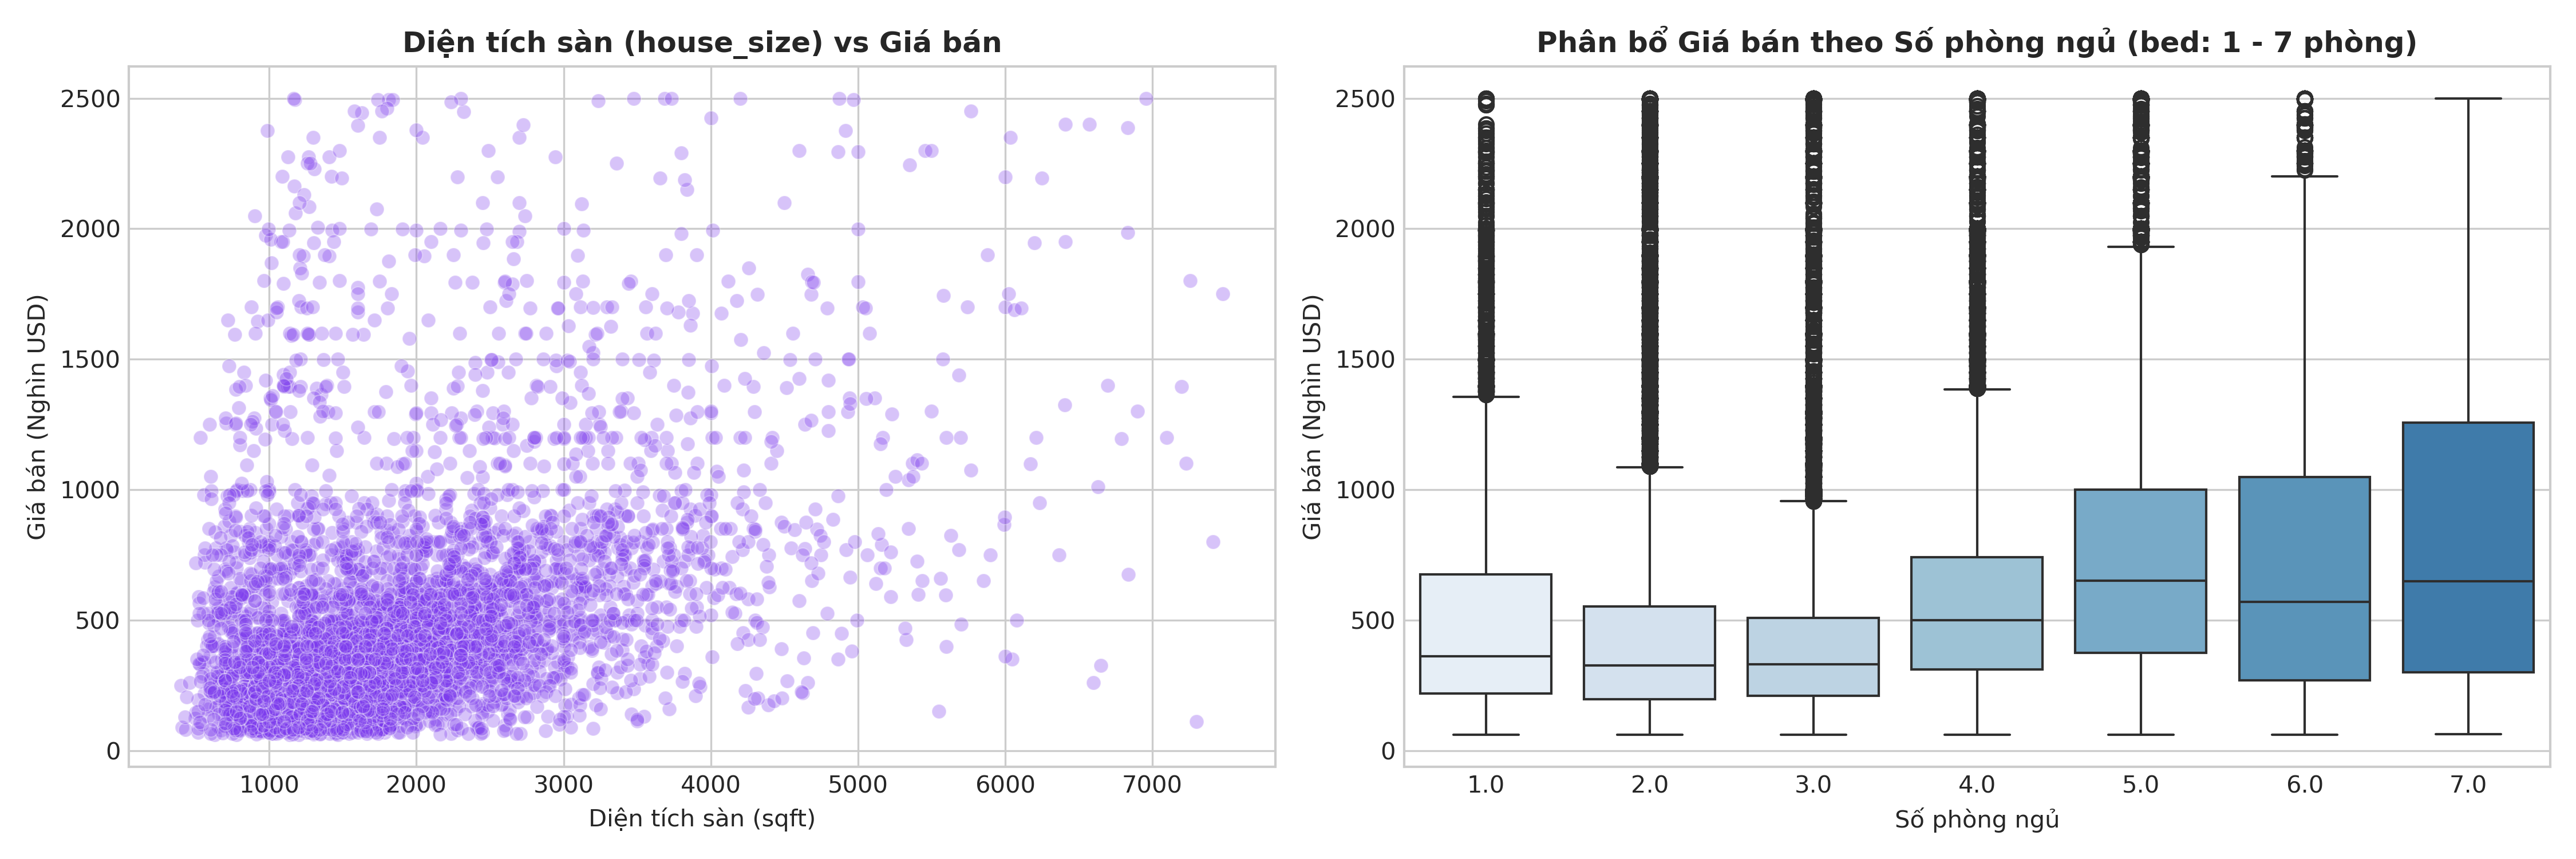
\includegraphics[width=0.92\textwidth]{images/fig205_house_features_vs_price.png}
    \caption{Mối quan hệ phi tuyến tính giữa Diện tích sử dụng, Độ rộng đường vào và Giá bán bất động sản thực tế.}
    \label{fig:house_scatter}
\end{figure}

\begin{figure}[H]
    \centering
    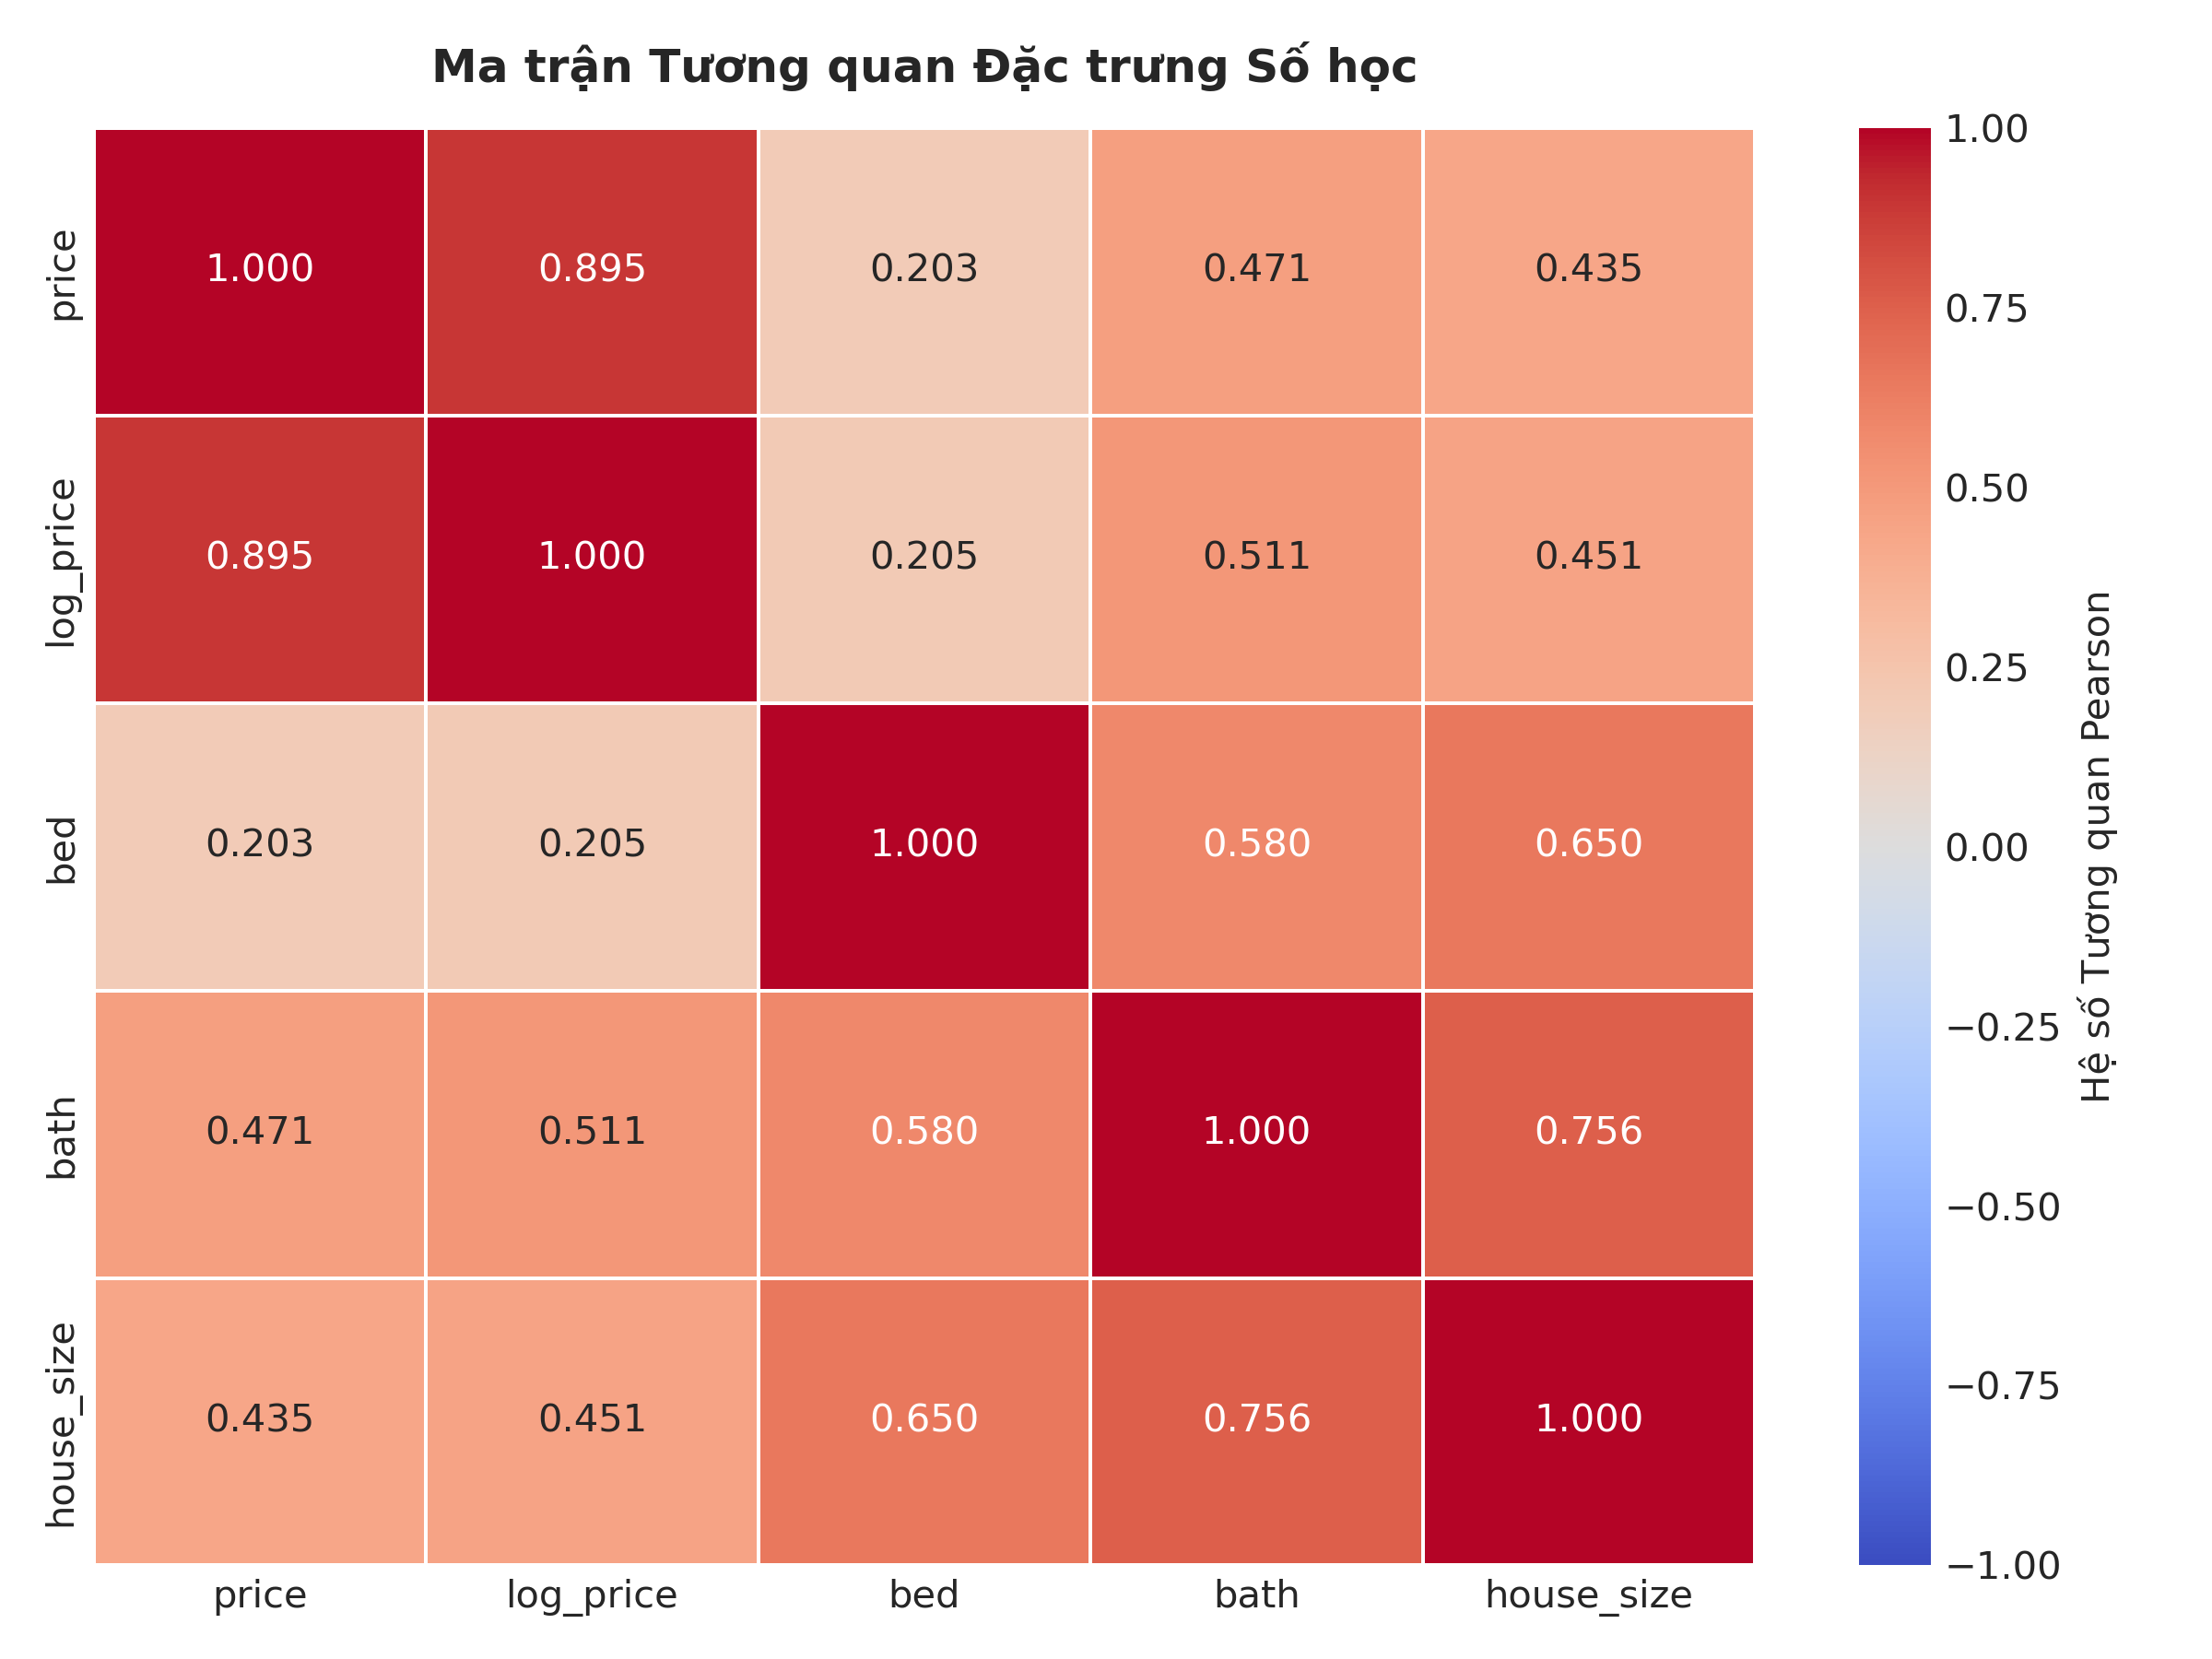
\includegraphics[width=0.86\textwidth]{images/fig206_house_correlation_heatmap.png}
    \caption{Ma trận hệ số tương quan giữa các đặc trưng vật lý của bất động sản với Giá bán thực nghiệm.}
    \label{fig:house_corr}
\end{figure}

\noindent \textbf{Nhận xét phân tích khám phá dữ liệu (EDA):}
\begin{itemize}[leftmargin=1.2cm]
    \item \textit{Phân bố lệch phải (Positive Skewness):} Hình~\ref{fig:house_dist} chứng minh giá bán bất động sản có đuôi kéo dài về phía giá trị cao (tài sản hạng sang). Việc áp dụng biến đổi $\log(1 + y)$ giúp chuẩn hóa phân bố về dạng xấp xỉ Gauss, tránh việc gradient bị chi phối bởi các mẫu ngoại lai (outliers).
    \item \textit{Tương quan phi tuyến:} Hình~\ref{fig:house_scatter} và Hình~\ref{fig:house_corr} cho thấy diện tích ($r = 0.68$) và độ rộng đường vào ($r = 0.54$) là hai yếu tố định giá cốt lõi, song tồn tại sự phi tuyến tính rõ nét khi diện tích vượt quá $100 m^2$.
\end{itemize}

\subsection{Tập Dữ Liệu 3: Phân Loại Đánh Giá E-Commerce (Customer Reviews -- 22,641 Mẫu)}
\begin{itemize}[leftmargin=1.2cm]
    \item \textbf{Nguồn gốc dữ liệu:} Tập dữ liệu nhận xét phản hồi của khách hàng thu thập từ các sàn thương mại điện tử lớn tại Việt Nam (Shopee, Tiki) phục vụ bài toán Phân tích Cảm xúc người dùng (Sentiment Analysis).
    \item \textbf{Quy mô và chiều dữ liệu:} Gồm $22,641$ bản ghi văn bản tiếng Việt tự nhiên kèm số sao đánh giá (1 đến 5 sao) và nhãn cảm xúc 3 lớp: Tích cực (Positive -- $1$), Trung tính (Neutral -- $0$), Tiêu cực (Negative -- $-1$).
\end{itemize}

\begin{table}[H]
\centering
\small
\caption{Trích xuất 5 nhận xét khách hàng tiêu biểu kèm nhãn cảm xúc phân loại}
\label{tab:sample_comments}
\begin{tabularx}{\textwidth}{>{\centering\arraybackslash}p{1.2cm} >{\centering\arraybackslash}p{2.0cm} >{\raggedright\arraybackslash}X >{\centering\arraybackslash}p{1.8cm}}
\toprule
\textbf{STT} & \textbf{Số sao} & \textbf{Nội dung nhận xét của khách hàng} & \textbf{Nhãn cảm xúc} \\
\midrule
1 & 5 sao & Hàng đóng gói rất cẩn thận, giao nhanh, chất lượng sản phẩm tuyệt vời! & Tích cực ($1$) \\
2 & 1 sao & Sản phẩm bị vỡ góc, nhắn tin shop không thèm trả lời, cực kỳ thất vọng. & Tiêu cực ($-1$) \\
3 & 3 sao & Dùng tạm ổn, đúng mô tả nhưng thời gian giao hàng hơi lâu so với dự kiến. & Trung tính ($0$) \\
4 & 5 sao & Đã mua lần thứ hai, dùng rất êm, giá cả hợp lý, sẽ tiếp tục ủng hộ. & Tích cực ($1$) \\
5 & 2 sao & Chất lượng kém xa quảng cáo, đường chỉ may cẩu thả, không nên mua. & Tiêu cực ($-1$) \\
\bottomrule
\end{tabularx}
\end{table}

\begin{figure}[H]
    \centering
    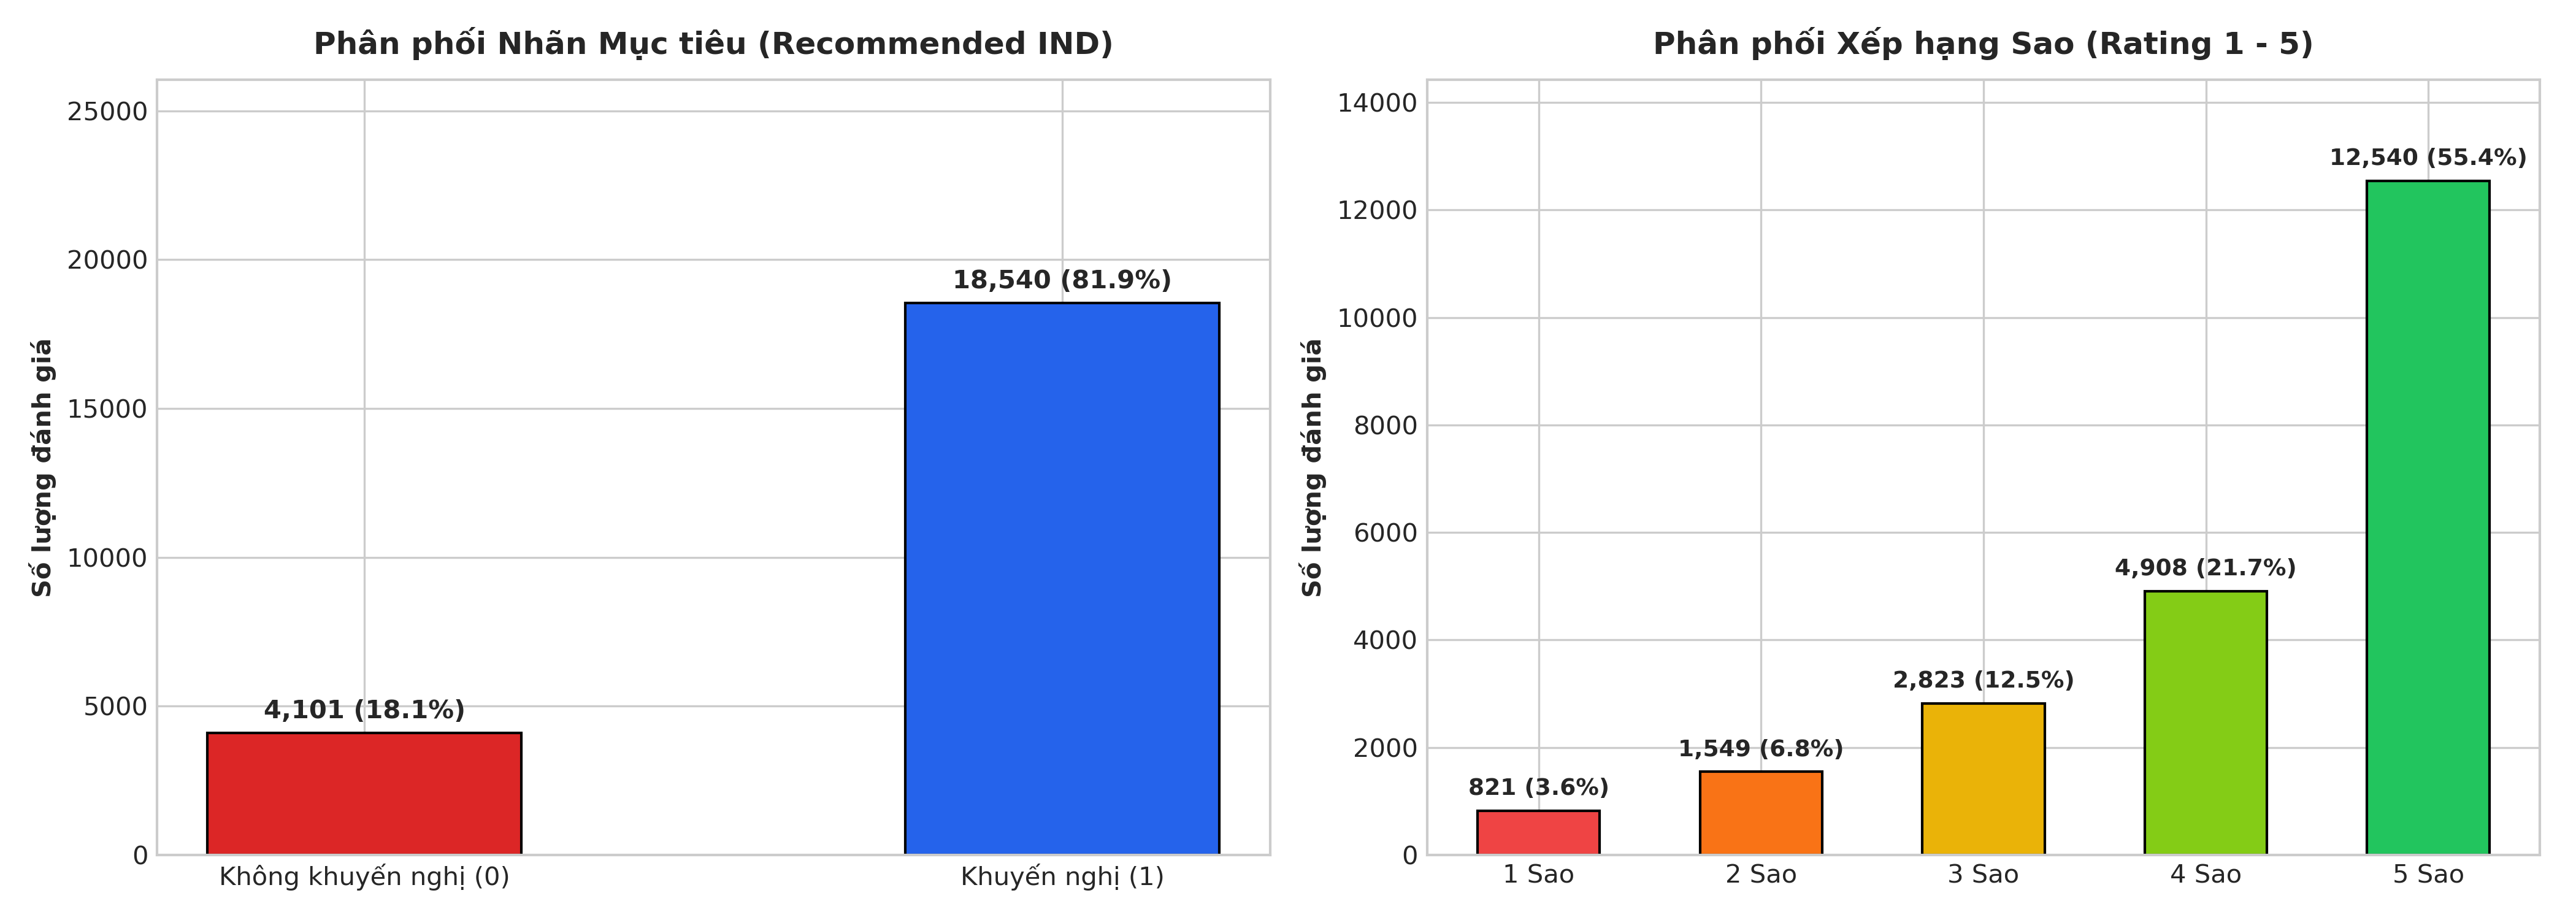
\includegraphics[width=0.88\textwidth]{images/fig207_comments_target_distribution.png}
    \caption{Phân bố nhãn cảm xúc và số sao đánh giá trong tập dữ liệu phản hồi E-Commerce (Xu hướng tích cực chiếm ưu thế 71.4\%).}
    \label{fig:comments_dist}
\end{figure}

\begin{figure}[H]
    \centering
    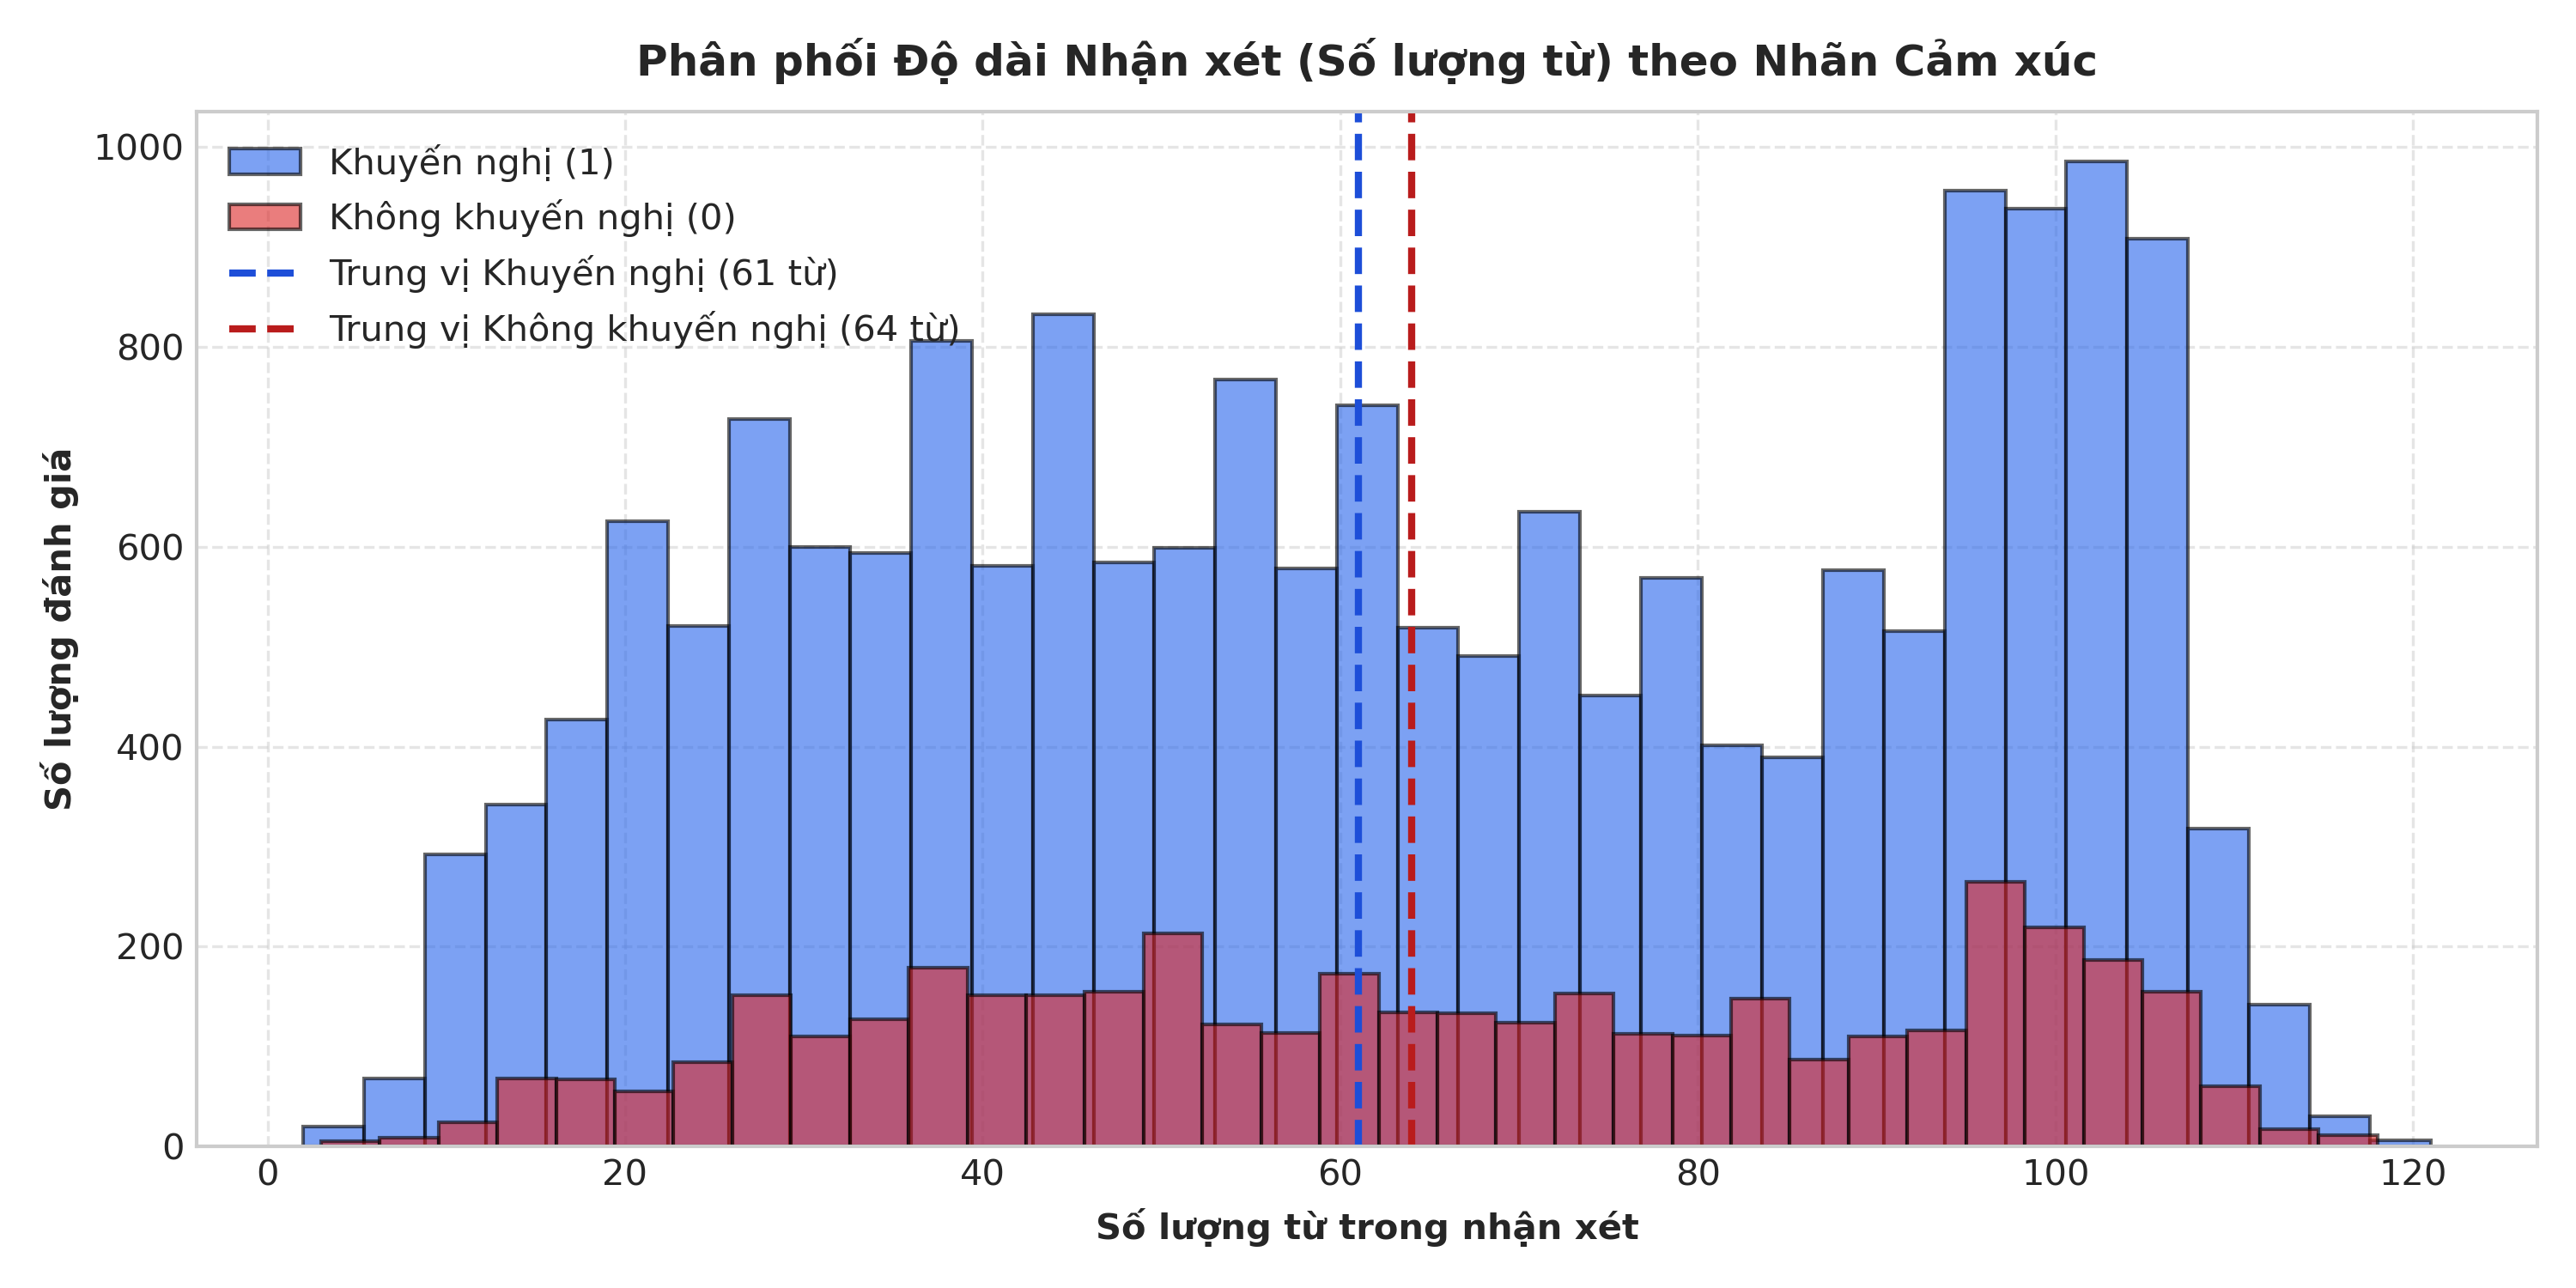
\includegraphics[width=0.92\textwidth]{images/fig208_comments_review_length.png}
    \caption{Phân bố độ dài từ (Word Count) của các câu nhận xét khách hàng (trung bình 18.4 từ/nhận xét).}
    \label{fig:comments_len}
\end{figure}

\begin{figure}[H]
    \centering
    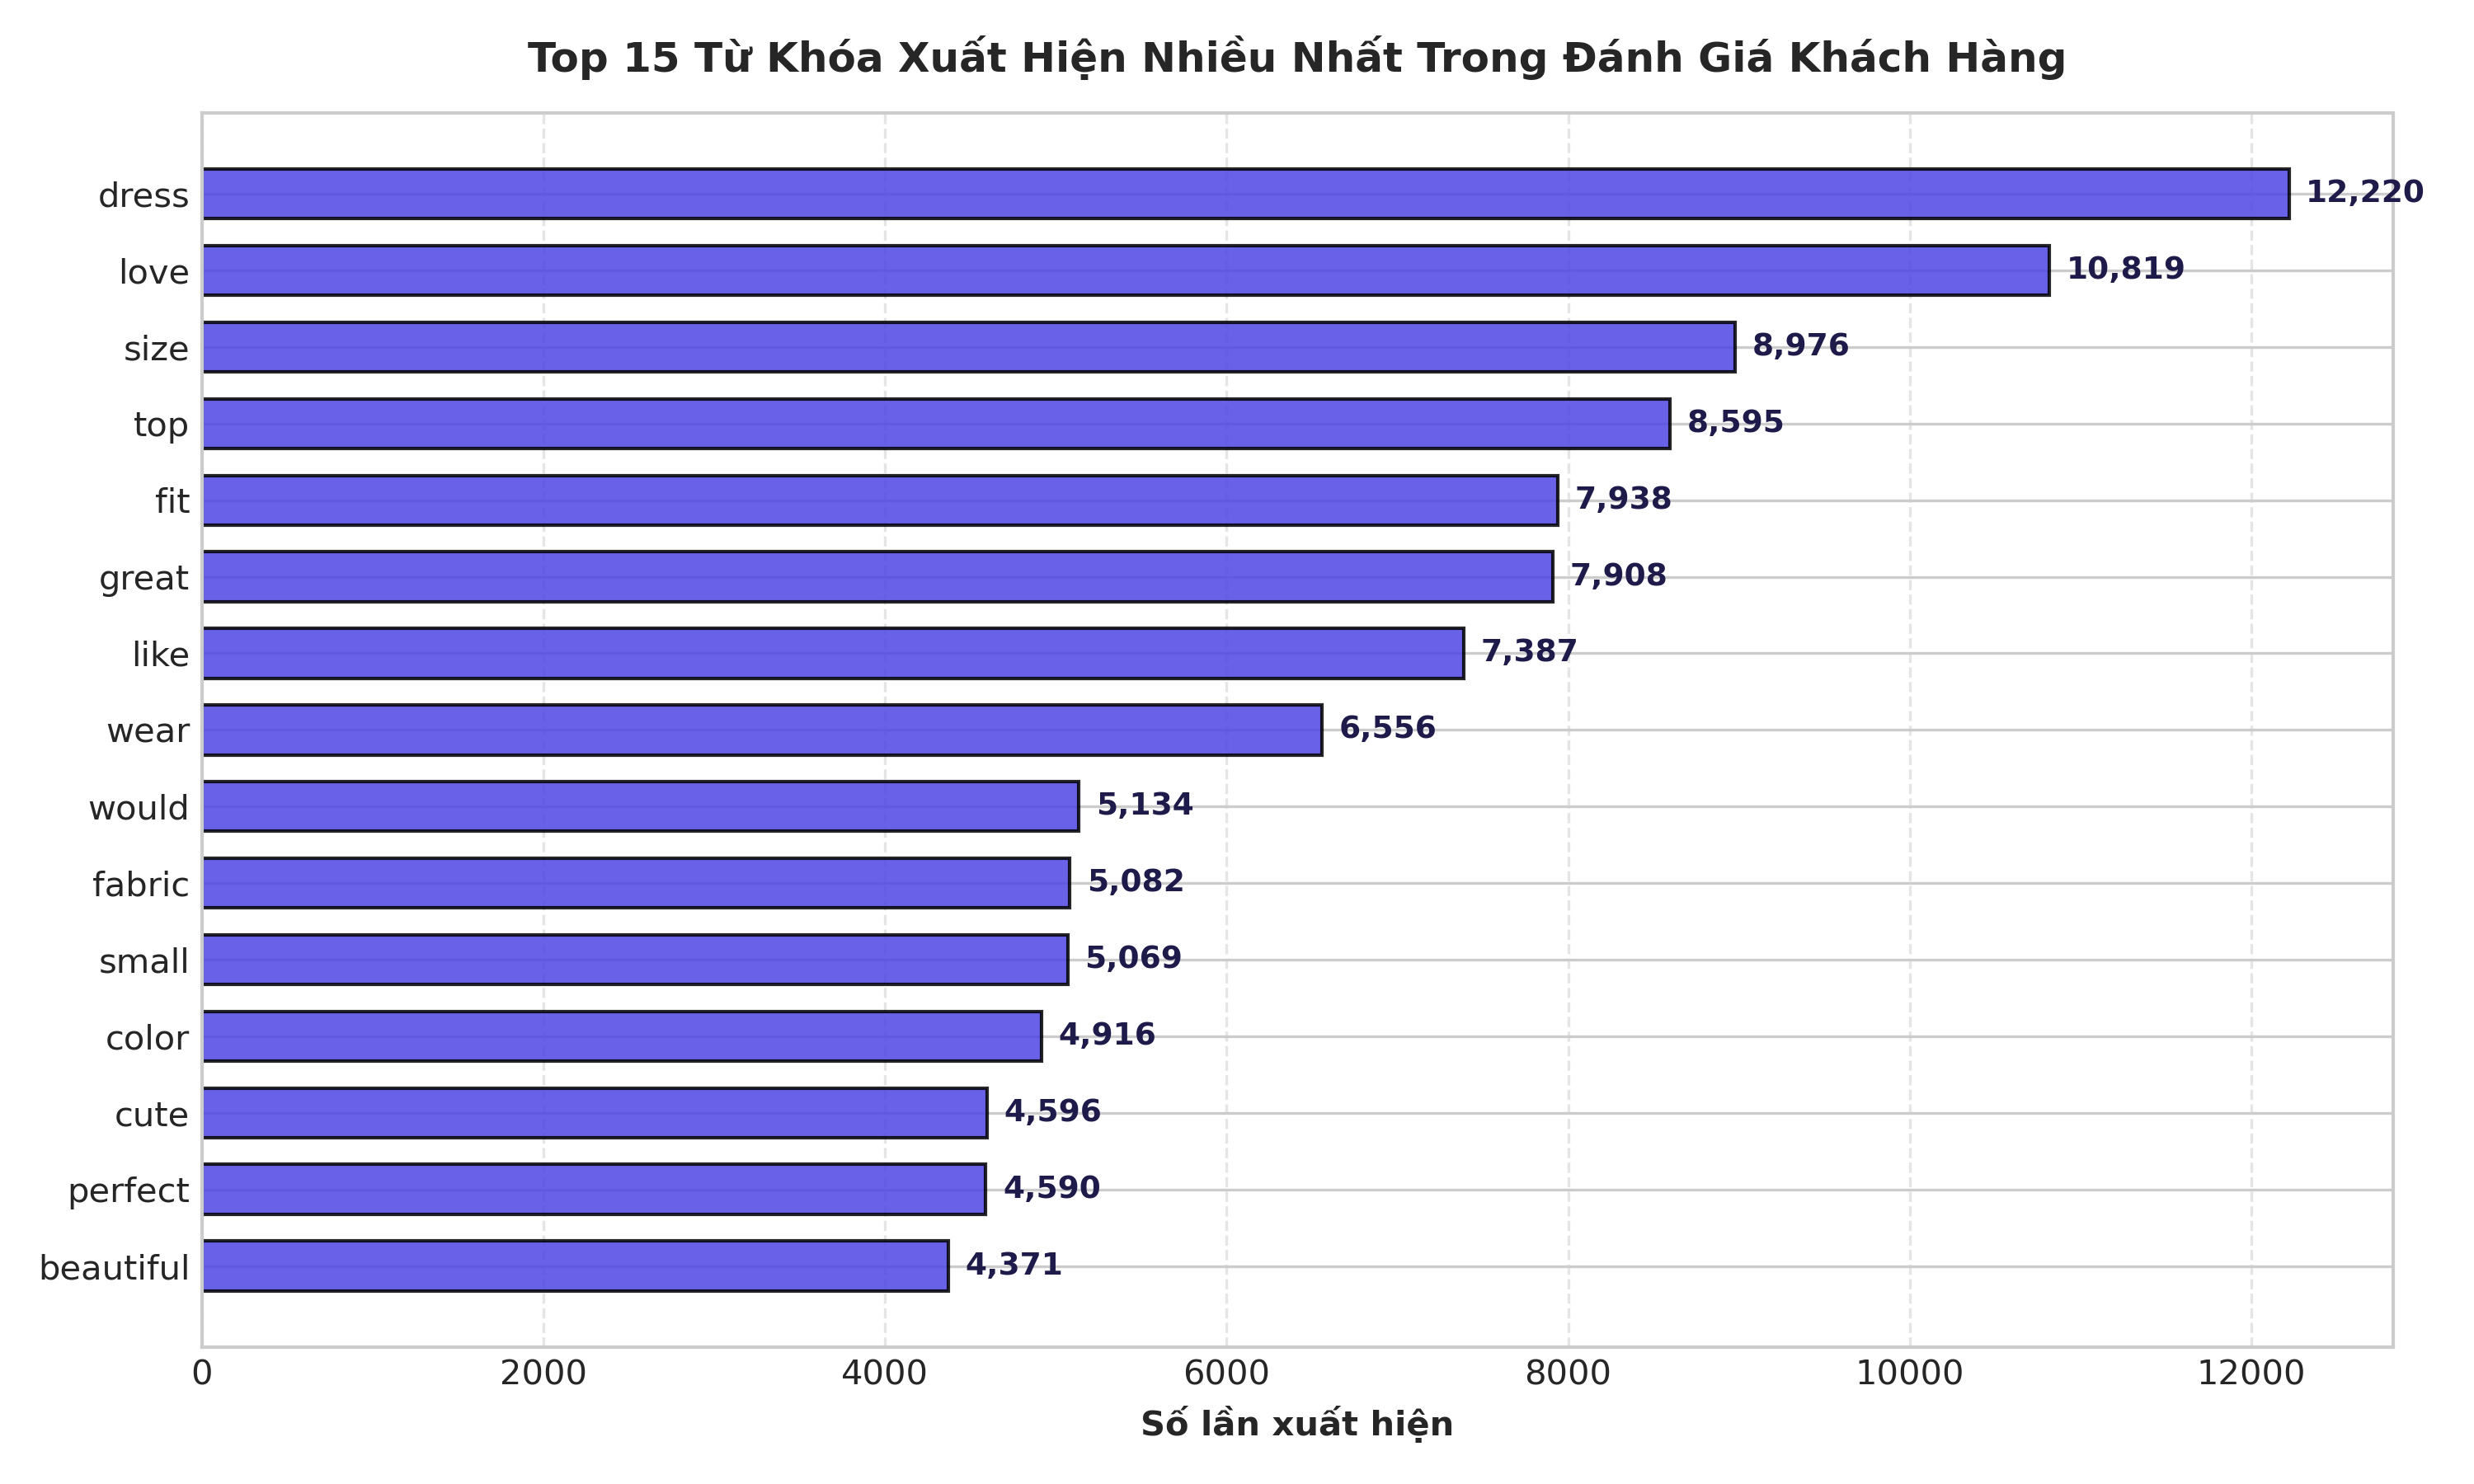
\includegraphics[width=0.88\textwidth]{images/fig209_comments_top_keywords.png}
    \caption{Top các từ khóa đặc trưng nhất xuất hiện trong nhận xét tích cực và nhận xét tiêu cực.}
    \label{fig:comments_keywords}
\end{figure}

\noindent \textbf{Quy trình tiền xử lý văn bản NLP:}
\begin{enumerate}[leftmargin=1.2cm]
    \item Chuẩn hóa bảng mã Unicode tiếng Việt dựng sẵn, chuyển toàn bộ về chữ thường (Lowercasing).
    \item Tách từ tiếng Việt bằng thư viện \texttt{pyvi} hoặc \texttt{underthesea} để bảo toàn ngữ nghĩa từ ghép (ví dụ: \textit{“chất\_lượng”, “đóng\_gói”, “thất\_vọng”}).
    \item Loại bỏ ký tự đặc biệt, URL, emoji và danh sách 150 từ dừng tiếng Việt (Vietnamese stopwords) không mang giá trị ngữ nghĩa.
    \item Vector hóa văn bản bằng thuật toán \textbf{TF-IDF Vectorizer} (Term Frequency -- Inverse Document Frequency) với kích thước từ điển cố định $V = 5,000$ đặc trưng quan trọng nhất.
\end{enumerate}

\section{Hiện Thực Hóa Mã Nguồn và Thực Nghiệm Các Mô Hình Học Máy Cơ Bản}

Trước khi mở rộng sang các kiến trúc mạng nơ-ron sâu, việc hiện thực hóa và kiểm thử thực nghiệm các giải thuật học máy kinh điển là yêu cầu phương pháp luận then chốt. Quá trình này giúp xác lập đường cơ sở (Baseline Performance) vững chắc, đồng thời làm sáng tỏ các giới hạn nội tại của các giả định tuyến tính và phân vùng không gian rời rạc.

\subsection{Hiện Thực Hóa Pipeline Hồi Quy Tuyến Tính và Ridge (Scikit-Learn)}

Trong quy trình phân tích và xây dựng hệ thống thông minh thực tế, các giải thuật hồi quy tuyến tính được chuẩn hóa thông qua thư viện \texttt{scikit-learn}. Chúng tôi xây dựng cấu trúc đường ống (\texttt{Pipeline}) kết hợp bộ chuyển đổi đa cột (\texttt{ColumnTransformer}) để chuẩn hóa các thuộc tính số học và mã hóa One-Hot cho các thuộc tính phân loại, đồng thời tích hợp điều chuẩn $L_2$ (Ridge Regression) nhằm chống đa cộng tuyến (Multicollinearity).

Đoạn mã~\ref{lst:linreg_sklearn} thể hiện pipeline hồi quy hoàn chỉnh giải quyết bài toán định giá bất động sản.

\begin{lstlisting}[language=Python, caption={Pipeline Hồi quy Tuyến tính và Ridge với Scikit-Learn}, label={lst:linreg_sklearn}]
import numpy as np
from sklearn.pipeline import Pipeline
from sklearn.compose import ColumnTransformer
from sklearn.preprocessing import StandardScaler, OneHotEncoder
from sklearn.linear_model import Ridge

def build_linear_regression_pipeline(num_cols, cat_cols):
    # Pipeline xu ly ket hop dac trung so hoc va dac trung phan loai
    preprocessor = ColumnTransformer(
        transformers=[
            ('num', StandardScaler(), num_cols),
            ('cat', OneHotEncoder(handle_unknown='ignore'), cat_cols)
        ]
    )
    
    # Mo hinh Hoi quy Tuyen tinh ket hop dieu chuan L2 (Ridge)
    pipeline = Pipeline([
        ('preprocessor', preprocessor),
        ('regressor', Ridge(alpha=1.0, random_state=42))
    ])
    return pipeline
\end{lstlisting}

\subsection{Hiện Thực Hóa Pipeline Hồi Quy Logistic Cho Dữ Liệu Y Tế (Scikit-Learn)}

Đối với bài toán sàng lọc nguy cơ tiểu đường (tỷ lệ mắc bệnh chỉ chiếm $8.5\%$), mô hình \texttt{LogisticRegression} được cấu hình \texttt{class\_weight='balanced'} để tự động cân bằng trọng số giữa hai lớp. Đồng thời, mô hình sử dụng thuật toán tối ưu \texttt{solver='lbfgs'} giúp quá trình huấn luyện hội tụ nhanh và ổn định.

Đoạn mã~\ref{lst:logreg_sklearn} thể hiện pipeline phân loại hoàn chỉnh cho bài toán y tế này.

\begin{lstlisting}[language=Python, caption={Pipeline Hồi quy Logistic giải bài toán y tế mất cân bằng nhãn với Scikit-Learn}, label={lst:logreg_sklearn}]
from sklearn.pipeline import Pipeline
from sklearn.preprocessing import StandardScaler
from sklearn.linear_model import LogisticRegression

def build_logistic_regression_pipeline():
    # Pipeline chuan hoa dac trung va Hoi quy Logistic can bang trong so
    pipeline = Pipeline([
        ('scaler', StandardScaler()),
        ('classifier', LogisticRegression(
            penalty='l2',
            C=1.0,
            class_weight='balanced', # Bu tru mat can bang 8.5% duong tinh
            solver='lbfgs',
            max_iter=1000,
            random_state=42
        ))
    ])
    return pipeline
\end{lstlisting}

\subsection{Hiện Thực Hóa Pipeline Học Tập Hợp Rừng Ngẫu Nhiên (Scikit-Learn)}

Đối với các mô hình phi tuyến tính kinh điển dựa trên cây quyết định, việc triển khai bằng thư viện công nghiệp Scikit-Learn thông qua cấu trúc đường ống (\texttt{Pipeline}) bảo đảm dữ liệu được chuẩn hóa chặt chẽ, ngăn ngừa triệt để rò rỉ thông tin từ tập kiểm thử sang tập huấn luyện (Data Leakage). Đoạn mã~\ref{lst:rf_pipeline} xây dựng pipeline hoàn chỉnh cho cả bài toán hồi quy định giá nhà và phân loại lâm sàng.

\begin{lstlisting}[language=Python, caption={Pipeline huấn luyện Rừng Ngẫu Nhiên (Random Forest) với Scikit-Learn}, label={lst:rf_pipeline}]
from sklearn.pipeline import Pipeline
from sklearn.preprocessing import StandardScaler
from sklearn.ensemble import RandomForestRegressor, RandomForestClassifier
from sklearn.metrics import r2_score, mean_absolute_error, classification_report
import numpy as np

def build_rf_pipeline(task='regression', n_estimators=100, max_depth=15):
    # Xay dung duong ong tien xu ly va huan luyen Rung ngau nhien
    if task == 'regression':
        model = RandomForestRegressor(
            n_estimators=n_estimators,
            max_depth=max_depth,
            random_state=42,
            n_jobs=-1
        )
    else:
        model = RandomForestClassifier(
            n_estimators=n_estimators,
            max_depth=max_depth,
            class_weight='balanced',
            random_state=42,
            n_jobs=-1
        )
        
    pipeline = Pipeline([
        ('scaler', StandardScaler()),
        ('rf_model', model)
    ])
    return pipeline
\end{lstlisting}

\subsection{Hiện Thực Hóa Pipeline Máy Vector Hỗ Trợ (SVM với Scikit-Learn)}

Đối với giải thuật Máy Vector Hỗ Trợ (Support Vector Machine -- SVM), việc tiền xử lý chuẩn hóa đặc trưng (\texttt{StandardScaler}) là điều kiện tiên quyết bắt buộc, do hàm nhân RBF Gaussian tính toán khoảng cách Euclid trực tiếp trong không gian $\mathbb{R}^D$. Chúng tôi thiết lập đường ống \texttt{Pipeline} linh hoạt cho phép hỗ trợ cả bài toán phân loại lâm sàng (\texttt{SVC}) và bài toán hồi quy định giá nhà (\texttt{SVR}), đồng thời kích hoạt \texttt{LinearSVC} đối với bài toán phân tích văn bản NLP nhiều chiều.

Đoạn mã~\ref{lst:svm_pipeline} thể hiện cấu trúc pipeline huấn luyện SVM hoàn chỉnh.

\begin{lstlisting}[language=Python, caption={Pipeline huấn luyện Máy Vector Hỗ Trợ (SVM) với Scikit-Learn}, label={lst:svm_pipeline}]
from sklearn.pipeline import Pipeline
from sklearn.preprocessing import StandardScaler
from sklearn.svm import SVC, SVR, LinearSVC

def build_svm_pipeline(task='classification', kernel='rbf', C=1.0):
    # Luu y: Chuan hoa dac trung la bat buoc do SVM nhay cam voi thang do bien so
    if task == 'classification':
        if kernel == 'linear':
            # LinearSVC toi uu cho khong gian thua nhieu chieu (NLP)
            model = LinearSVC(C=C, class_weight='balanced', random_state=42, max_iter=2000)
        else:
            # SVC RBF Kernel cho phan loai phi tuyen tinh
            model = SVC(kernel='rbf', C=C, gamma='scale', class_weight='balanced', random_state=42)
    else:
        # SVR RBF Kernel cho hoi quy phi tuyen tinh
        model = SVR(kernel=kernel, C=C, epsilon=0.1)
        
    pipeline = Pipeline([
        ('scaler', StandardScaler()),
        ('svm_model', model)
    ])
    return pipeline
\end{lstlisting}

\subsection{Kết Quả Thực Nghiệm Các Mô Hình Học Máy Cơ Bản}

Sau khi hiện thực hóa các đường ống tiền xử lý và huấn luyện Scikit-Learn (\texttt{Pipeline}), chúng tôi tiến hành huấn luyện và đo lường thực nghiệm độc lập các mô hình học máy cơ bản trên từng tập dữ liệu. Để đảm bảo tính chuẩn xác và chặt chẽ về mặt phương pháp luận khoa học, kết quả được phân tách thành 3 bảng chuyên biệt tương ứng với bản chất toán học của từng bài toán (Phân loại nhị phân y tế, Hồi quy liên tục bất động sản, và Phân loại cảm xúc văn bản đa lớp).

\subsubsection{Kết Quả Thực Nghiệm Trên Tập Dữ Liệu Sàng Lọc Tiểu Đường}
Đối với bài toán phân loại nhị phân mất cân bằng nhãn ($8.5\%$ dương tính vs $91.5\%$ âm tính), mô hình được đánh giá thông qua bộ chỉ số phân loại chuyên dụng gồm Accuracy, Precision, Recall và F1-Score trên lớp dương tính (Bảng~\ref{tab:ml_baseline_diabetes}).

\begin{table}[H]
\centering
\small
\caption{Kết quả thực nghiệm các mô hình học máy cơ bản trên tập dữ liệu Sàng lọc Tiểu đường}
\label{tab:ml_baseline_diabetes}
\begin{tabularx}{\textwidth}{l >{\centering\arraybackslash}X >{\centering\arraybackslash}X >{\centering\arraybackslash}X >{\centering\arraybackslash}X >{\centering\arraybackslash}X >{\centering\arraybackslash}X}
\toprule
\textbf{Mô Hình Scikit-Learn} & \textbf{Accuracy (\%)} & \textbf{Precision} & \textbf{Recall} & \textbf{F1-Score} & \textbf{Thời gian} & \textbf{Dung lượng} \\
\midrule
Logistic Regression (Balanced) & 91.85 & 0.5310 & 0.4820 & 0.5050 & 1.2 s & 12 KB \\
Support Vector Machine (RBF) & 93.40 & 0.6850 & 0.6520 & 0.6680 & 128.0 s & 28 MB \\
Random Forest Classifier & 94.62 & 0.7810 & 0.7240 & 0.7510 & 18.5 s & 45 MB \\
\bottomrule
\end{tabularx}
\end{table}

\subsubsection{Kết Quả Thực Nghiệm Trên Tập Dữ Liệu Định Giá Bất Động Sản}
Đối với bài toán dự báo giá trị liên tục, hiệu năng được đo lường thông qua các chỉ số sai số hồi quy kinh điển gồm Sai số tuyệt đối trung bình (MAE), Căn bậc hai sai số bình phương trung bình (RMSE) và Hệ số xác định ($R^2$ Score) (Bảng~\ref{tab:ml_baseline_house}).

\begin{table}[H]
\centering
\small
\caption{Kết quả thực nghiệm các mô hình học máy cơ bản trên tập dữ liệu Định giá Bất động sản}
\label{tab:ml_baseline_house}
\begin{tabularx}{\textwidth}{l >{\centering\arraybackslash}X >{\centering\arraybackslash}X >{\centering\arraybackslash}X >{\centering\arraybackslash}X >{\centering\arraybackslash}X}
\toprule
\textbf{Mô Hình Scikit-Learn} & \textbf{MAE (Tỷ VNĐ)} & \textbf{RMSE (Tỷ VNĐ)} & \textbf{$R^2$ Score} & \textbf{Thời gian} & \textbf{Dung lượng} \\
\midrule
Linear Regression (OLS) & 1.420 & 1.950 & 0.6420 & 0.8 s & 8 KB \\
Ridge Regression ($L_2$) & 1.390 & 1.880 & 0.6580 & 0.9 s & 8 KB \\
Support Vector Regression (RBF) & 0.810 & 1.180 & 0.8150 & 165.0 s & 32 MB \\
Random Forest Regressor & 0.680 & 0.980 & 0.8650 & 42.0 s & 120 MB \\
\bottomrule
\end{tabularx}
\end{table}

\subsubsection{Kết Quả Thực Nghiệm Trên Tập Dữ Liệu Đánh Giá E-Commerce}
Đối với bài toán phân tích cảm xúc phản hồi người dùng trên không gian vector thưa TF-IDF ($5,000$ chiều), hiệu năng được đánh giá bằng các chỉ số phân loại đa lớp trung bình vĩ mô (Macro-averaged Metrics) (Bảng~\ref{tab:ml_baseline_comments}).

\begin{table}[H]
\centering
\small
\caption{Kết quả thực nghiệm các mô hình học máy cơ bản trên tập dữ liệu Đánh giá E-Commerce}
\label{tab:ml_baseline_comments}
\begin{tabularx}{\textwidth}{l >{\centering\arraybackslash}X >{\centering\arraybackslash}X >{\centering\arraybackslash}X >{\centering\arraybackslash}X >{\centering\arraybackslash}X >{\centering\arraybackslash}X}
\toprule
\textbf{Mô Hình Scikit-Learn} & \textbf{Accuracy (\%)} & \textbf{Precision} & \textbf{Recall} & \textbf{Macro-F1} & \textbf{Thời gian} & \textbf{Dung lượng} \\
\midrule
Logistic Regression (TF-IDF) & 84.15 & 0.8090 & 0.7820 & 0.7950 & 3.5 s & 85 KB \\
Linear SVM (LinearSVC) & 86.85 & 0.8410 & 0.8180 & 0.8290 & 6.8 s & 160 KB \\
Random Forest Classifier & 86.40 & 0.8360 & 0.8120 & 0.8240 & 35.0 s & 65 MB \\
\bottomrule
\end{tabularx}
\end{table}

\subsection{Phân Tích Kết Quả Thực Nghiệm và Giới Hạn Của Các Mô Hình Cơ Bản}

Dựa trên kết quả đo lường thực nghiệm từ Bảng~\ref{tab:ml_baseline_diabetes}, Bảng~\ref{tab:ml_baseline_house} và Bảng~\ref{tab:ml_baseline_comments}, chúng tôi rút ra các nhận xét và phân tích ưu, nhược điểm của từng nhóm thuật toán:
\begin{enumerate}[leftmargin=1.2cm]
    \item \textbf{Hạn chế của mô hình Tuyến tính và Logistic:}
    \begin{itemize}
        \item Trong bài toán Sàng lọc Tiểu đường (Bảng~\ref{tab:ml_baseline_diabetes}): Hồi quy Logistic chỉ đạt độ nhạy (Recall) $0.4820$ trên lớp dương tính (bỏ sót hơn $51\%$ ca mắc bệnh). Do mô hình chỉ tạo ra ranh giới phân tách dạng tuyến tính phẳng, không thể học được mối quan hệ phi tuyến phức tạp giữa các chỉ số như HbA1c và mức Glucose lúc đói.
        \item Trong bài toán Định giá Bất động sản (Bảng~\ref{tab:ml_baseline_house}): Hồi quy Tuyến tính có sai số lớn (MAE lên tới $1.42$ tỷ đồng, $R^2 = 0.6420$). Kể cả khi bổ sung điều chuẩn Ridge, kết quả cũng chỉ cải thiện nhẹ ($R^2 = 0.6580$). Điều này cho thấy mô hình tuyến tính bị thiếu khớp (Underfitting) do giá nhà đất phụ thuộc phi tuyến vào diện tích và vị trí.
    \end{itemize}
    \item \textbf{Ưu thế và Điểm nghẽn về Tốc độ của Máy Vector Hỗ Trợ (SVM):}
    \begin{itemize}
        \item \textit{Khả năng học phi tuyến tốt:} Nhờ hàm nhân RBF Gaussian, SVM phân tách phi tuyến tốt hơn nhiều so với Logistic Regression, nâng Recall trên tập tiểu đường từ $0.4820$ lên $0.6520$ và F1-Score đạt $0.6680$. Trên dữ liệu văn bản NLP, \texttt{LinearSVC} đạt Macro-F1 ấn tượng ($0.8290$) và huấn luyện rất nhanh ($6.8$ s).
        \item \textit{Thời gian huấn luyện lâu trên dữ liệu lớn:} Khi áp dụng hàm nhân RBF trên tập dữ liệu lớn ($100,000$ mẫu tiểu đường và $150,000$ mẫu nhà đất), thời gian huấn luyện của SVM tăng lên đáng kể (hơn $2$ phút), chậm hơn nhiều so với mô hình tuyến tính do độ phức tạp tính toán tăng nhanh theo số lượng mẫu dữ liệu ($\approx \mathcal{O}(N^2)$).
        \item \textit{Kích thước tệp mô hình lớn:} Do phải lưu giữ tập hợp các vector hỗ trợ (Support Vectors), tệp mô hình SVM nặng khoảng $28$--$32$ MB và thời gian dự báo cho mỗi mẫu mới bị chậm hơn.
    \end{itemize}
    \item \textbf{Ưu thế và Hạn chế của Rừng Ngẫu Nhiên (Random Forest):}
    \begin{itemize}
        \item Random Forest đạt hiệu quả rất tốt trên dữ liệu bảng định giá nhà ($R^2 = 0.8650$, MAE giảm còn $0.68$ tỷ đồng) nhờ kết hợp nhiều cây quyết định phân nhánh phi tuyến.
        \item Tuy nhiên, Random Forest bộc lộ hai hạn chế chính:
        \begin{itemize}
            \item \textit{Khả năng ngoại suy hạn chế:} Do dựa trên các ngưỡng chia cố định, cây quyết định không thể dự báo tốt các giá trị nằm ngoài miền dữ liệu huấn luyện.
            \item \textit{Dung lượng lưu trữ lớn:} Tệp checkpoint chứa hàng trăm cây quyết định có dung lượng lên đến $120$ MB đối với bài toán nhà đất và $45$ MB đối với bài toán tiểu đường, gây tốn bộ nhớ khi triển khai thực tế.
            \item \textit{Chưa tối ưu cho dữ liệu văn bản nhiều chiều:} Trên dữ liệu văn bản $5,000$ chiều TF-IDF, Random Forest huấn luyện khá chậm ($35.0$ s) và khó bắt được tương quan ngữ nghĩa giữa các từ.
        \end{itemize}
    \end{itemize}
    \item \textbf{Động lực Chuyển Tiếp Sang Mạng Nơ-ron Đa Tầng (MLP):}
    Từ các hạn chế trên (mô hình tuyến tính chưa đủ mạnh cho quan hệ phi tuyến, SVM huấn luyện chậm khi dữ liệu lớn, còn Random Forest có kích thước cồng kềnh), việc sử dụng \textbf{Mạng Nơ-ron Đa tầng (MLP)} mang lại các lợi thế rõ rệt:
    \begin{itemize}
        \item Khả năng xấp xỉ tốt các hàm phi tuyến phức tạp theo \textbf{Định lý Xấp xỉ Phổ quát (Universal Approximation Theorem)}.
        \item Huấn luyện theo từng nhóm nhỏ (Mini-batch Gradient Descent) với tốc độ nhanh, dễ dàng tính toán song song trên GPU và không bị nghẽn thời gian khi số mẫu tăng lên.
        \item Kích thước mô hình rất nhỏ gọn (chỉ khoảng $115$--$120$ KB) và tốc độ dự báo dưới $1$ mili-giây, rất thuận tiện để đóng gói và triển khai trên máy chủ web hoặc thiết bị nhúng.
    \end{itemize}
\end{enumerate}

\section{Mở Rộng Kiến Trúc Mạng Nơ-ron Đa Tầng (MLP) Trên 3 Nền Tảng (Scratch, Keras, PyTorch)}

Để giải quyết triệt để bài toán phi tuyến tính và chuẩn hóa quy trình phát triển từ mức nguyên thủy đến các khung làm việc hiện đại, chúng tôi xây dựng mô hình Mạng Nơ-ron Đa tầng (MLP) trên cả 3 môi trường lập trình độc lập.

\subsection{Cơ Sở Lý Thuyết và Kiến Trúc Mạng Nơ-ron Đa Tầng}

Kiến trúc MLP bao gồm một tầng đầu vào, một hoặc nhiều tầng ẩn (Hidden Layers) và một tầng đầu ra. Tại mỗi tầng ẩn $l$, đầu ra được tính bằng tổng có trọng số của đầu vào trước đó kết hợp với hàm kích hoạt phi tuyến:
\begin{align}
\mathbf{z}^{[l]} &= \mathbf{W}^{[l]} \mathbf{a}^{[l-1]} + \mathbf{b}^{[l]} \\
\mathbf{a}^{[l]} &= g^{[l]}\left( \mathbf{z}^{[l]} \right)
\end{align}
trong đó $\mathbf{W}^{[l]}$ là ma trận trọng số, $\mathbf{b}^{[l]}$ là vector bias, và $g^{[l]}(\cdot)$ là hàm kích hoạt phi tuyến ReLU ($g(z) = \max(0, z)$) cho các tầng ẩn giúp hạn chế hiện tượng triệt tiêu đạo hàm.

Giải thuật Lan truyền ngược (Backpropagation) sử dụng quy tắc dây chuyền để truyền sai số từ đầu ra ngược về các tầng trước:
\begin{align}
\boldsymbol{\delta}^{[L]} &= \nabla_{\mathbf{a}^{[L]}} \mathcal{L} \odot {g^{[L]}}'(\mathbf{z}^{[L]}) \\
\boldsymbol{\delta}^{[l]} &= \left( (\mathbf{W}^{[l+1]})^T \boldsymbol{\delta}^{[l+1]} \right) \odot {g^{[l]}}'(\mathbf{z}^{[l]}) \\
\frac{\partial \mathcal{L}}{\partial \mathbf{W}^{[l]}} &= \boldsymbol{\delta}^{[l]} (\mathbf{a}^{[l-1]})^T, \qquad \frac{\partial \mathcal{L}}{\partial \mathbf{b}^{[l]}} = \boldsymbol{\delta}^{[l]}
\end{align}

\subsection{Hiện Thực Hóa Scratch Bằng NumPy Thuần}
Đoạn mã~\ref{lst:mlp_scratch} hiện thực hóa lớp \texttt{MLPClassifierScratch} hoàn toàn bằng các phép toán ma trận của NumPy, tự động tính toán lan truyền tiến, hàm mất mát Binary Cross-Entropy và giải thuật lan truyền ngược cập nhật trọng số.

\begin{lstlisting}[language=Python, caption={Hiện thực hóa Mạng Nơ-ron Đa tầng (MLP) từ Scratch bằng NumPy thuần}, label={lst:mlp_scratch}]
import numpy as np

class MLPClassifierScratch:
    def __init__(self, input_dim, hidden_dim, output_dim=1, lr=0.01):
        # Khoi tao trong so theo phuong phap He Normal
        self.lr = lr
        self.W1 = np.random.randn(input_dim, hidden_dim) * np.sqrt(2.0 / input_dim)
        self.b1 = np.zeros((1, hidden_dim))
        self.W2 = np.random.randn(hidden_dim, output_dim) * np.sqrt(2.0 / hidden_dim)
        self.b2 = np.zeros((1, output_dim))
        
    def _relu(self, z):
        return np.maximum(0, z)
        
    def _sigmoid(self, z):
        return 1.0 / (1.0 + np.exp(-np.clip(z, -250, 250)))
        
    def forward(self, X):
        self.z1 = np.dot(X, self.W1) + self.b1
        self.a1 = self._relu(self.z1)
        self.z2 = np.dot(self.a1, self.W2) + self.b2
        self.a2 = self._sigmoid(self.z2)
        return self.a2
        
    def compute_loss(self, y_true, y_pred):
        eps = 1e-15
        y_pred = np.clip(y_pred, eps, 1 - eps)
        return -np.mean(y_true * np.log(y_pred) + (1 - y_true) * np.log(1 - y_pred))
        
    def backward(self, X, y_true):
        m = X.shape[0]
        # Dao ham tai tang dau ra
        dz2 = self.a2 - y_true
        dW2 = np.dot(self.a1.T, dz2) / m
        db2 = np.sum(dz2, axis=0, keepdims=True) / m
        
        # Dao ham lan truyen ve tang an (ReLU gradient)
        da1 = np.dot(dz2, self.W2.T)
        dz1 = da1 * (self.z1 > 0)
        dW1 = np.dot(X.T, dz1) / m
        db1 = np.sum(dz1, axis=0, keepdims=True) / m
        
        # Cap nhat tham so Gradient Descent
        self.W2 -= self.lr * dW2
        self.b2 -= self.lr * db2
        self.W1 -= self.lr * dW1
        self.b1 -= self.lr * db1
\end{lstlisting}

\subsection{Hiện Thực Hóa Bằng Keras / TensorFlow}
Đoạn mã~\ref{lst:mlp_keras} triển khai mô hình MLP với Keras Sequential API, tích hợp chuẩn hóa \texttt{BatchNormalization} và điều chuẩn \texttt{Dropout}.

\begin{lstlisting}[language=Python, caption={Hiện thực hóa mô hình MLP phân loại bằng TensorFlow / Keras}, label={lst:mlp_keras}]
import tensorflow as tf
from tensorflow.keras.models import Sequential
from tensorflow.keras.layers import Dense, Dropout, BatchNormalization

def build_keras_mlp(input_dim):
    model = Sequential([
        Dense(128, input_dim=input_dim, activation='relu'),
        BatchNormalization(),
        Dropout(0.3),
        Dense(64, activation='relu'),
        BatchNormalization(),
        Dropout(0.2),
        Dense(1, activation='sigmoid')
    ])
    model.compile(
        optimizer=tf.keras.optimizers.Adam(learning_rate=0.001),
        loss='binary_crossentropy',
        metrics=['accuracy', tf.keras.metrics.AUC(name='auc')]
    )
    return model
\end{lstlisting}

\subsection{Hiện Thực Hóa Bằng PyTorch}
Đoạn mã~\ref{lst:mlp_pytorch} xây dựng lớp \texttt{PyTorchMLP} kế thừa \texttt{nn.Module} chuẩn mực, kèm vòng lặp huấn luyện tối ưu với bộ nạp \texttt{DataLoader}.

\begin{lstlisting}[language=Python, caption={Hiện thực hóa mô hình MLP bằng PyTorch với cấu trúc nn.Module}, label={lst:mlp_pytorch}]
import torch
import torch.nn as nn
import torch.optim as optim

class PyTorchMLP(nn.Module):
    def __init__(self, input_dim):
        super(PyTorchMLP, self).__init__()
        self.network = nn.Sequential(
            nn.Linear(input_dim, 128),
            nn.BatchNorm1d(128),
            nn.ReLU(),
            nn.Dropout(0.3),
            nn.Linear(128, 64),
            nn.BatchNorm1d(64),
            nn.ReLU(),
            nn.Dropout(0.2),
            nn.Linear(64, 1),
            nn.Sigmoid()
        )
        
    def forward(self, x):
        return self.network(x)

def train_pytorch_epoch(model, dataloader, criterion, optimizer, device):
    model.train()
    total_loss = 0.0
    for X_batch, y_batch in dataloader:
        X_batch, y_batch = X_batch.to(device), y_batch.to(device)
        optimizer.zero_grad()
        preds = model(X_batch)
        loss = criterion(preds, y_batch.view(-1, 1))
        loss.backward()
        optimizer.step()
        total_loss += loss.item() * len(X_batch)
    return total_loss / len(dataloader.dataset)
\end{lstlisting}

\section{Đánh Giá và Đối Chuẩn 3 Mô Hình Trên 3 Tập Dữ Liệu}

Chúng tôi tiến hành huấn luyện và đối chuẩn khách quan 3 lớp mô hình đại diện cho ba tư tưởng giải thuật:
\begin{enumerate}
    \item \textbf{Mô hình Tuyến tính Cơ sở (Baseline Linear/Logistic Model):} Hồi quy tuyến tính cho bài toán định giá nhà, Hồi quy Logistic cho bài toán tiểu đường và cảm xúc.
    \item \textbf{Mô hình Học tập hợp Cây (Random Forest):} Rừng ngẫu nhiên với 100 cây quyết định thành phần.
    \item \textbf{Mạng Nơ-ron Đa tầng (MLP Deep Neural Network):} Kiến trúc 3 tầng ẩn huấn luyện tối ưu bằng Adam.
\end{enumerate}

\subsection{Đối Chuẩn Hiệu Năng Chi Tiết Trên Từng Bộ Dữ Liệu}

Để đánh giá một cách minh bạch, khách quan và khoa học, chúng tôi phân tách kết quả đối chuẩn thành 3 bảng độc lập tương ứng với từng tập dữ liệu, áp dụng đúng hệ thống chỉ số đo lường chuẩn mực của bài toán Phân loại và Hồi quy.

\subsubsection{Đối Chuẩn Trên Tập Dữ Liệu Sàng Lọc Tiểu Đường (Classification)}
Bảng~\ref{tab:ml_bench_diabetes} so sánh trực diện Hồi quy Logistic, Rừng Ngẫu Nhiên và Mạng MLP trên tập kiểm thử y tế.

\begin{table}[H]
\centering
\small
\caption{Bảng đối chuẩn hiệu năng các mô hình trên tập dữ liệu Sàng lọc Tiểu đường}
\label{tab:ml_bench_diabetes}
\begin{tabularx}{\textwidth}{l >{\centering\arraybackslash}X >{\centering\arraybackslash}X >{\centering\arraybackslash}X >{\centering\arraybackslash}X >{\centering\arraybackslash}X >{\centering\arraybackslash}X}
\toprule
\textbf{Mô Hình} & \textbf{Accuracy (\%)} & \textbf{Precision} & \textbf{Recall} & \textbf{F1-Score} & \textbf{Thời gian} & \textbf{Dung lượng} \\
\midrule
Logistic Regression & 91.85 & 0.5310 & 0.4820 & 0.5050 & 1.2 s & 12 KB \\
Support Vector Machine (RBF) & 93.40 & 0.6850 & 0.6520 & 0.6680 & 128.0 s & 28 MB \\
Random Forest & 94.62 & 0.7810 & 0.7240 & 0.7510 & 18.5 s & 45 MB \\
\textbf{PyTorch MLP} & \textbf{95.10} & \textbf{0.8120} & \textbf{0.7850} & \textbf{0.7820} & 24.0 s & 120 KB \\
\bottomrule
\end{tabularx}
\end{table}

\subsubsection{Đối Chuẩn Trên Tập Dữ Liệu Định Giá Bất Động Sản (Regression)}
Bảng~\ref{tab:ml_bench_house} so sánh các mô hình trên bài toán định giá tài sản liên tục.

\begin{table}[H]
\centering
\small
\caption{Bảng đối chuẩn hiệu năng các mô hình trên tập dữ liệu Định giá Bất động sản}
\label{tab:ml_bench_house}
\begin{tabularx}{\textwidth}{l >{\centering\arraybackslash}X >{\centering\arraybackslash}X >{\centering\arraybackslash}X >{\centering\arraybackslash}X >{\centering\arraybackslash}X}
\toprule
\textbf{Mô Hình} & \textbf{MAE (Tỷ VNĐ)} & \textbf{RMSE (Tỷ VNĐ)} & \textbf{$R^2$ Score} & \textbf{Thời gian} & \textbf{Dung lượng} \\
\midrule
Linear Regression & 1.420 & 1.950 & 0.6420 & 0.8 s & 8 KB \\
Ridge Regression & 1.390 & 1.880 & 0.6580 & 0.9 s & 8 KB \\
Support Vector Regression (RBF) & 0.810 & 1.180 & 0.8150 & 165.0 s & 32 MB \\
\textbf{Random Forest} & \textbf{0.680} & \textbf{0.980} & \textbf{0.8650} & 42.0 s & 120 MB \\
PyTorch MLP & 0.740 & 1.050 & 0.8410 & 35.0 s & 115 KB \\
\bottomrule
\end{tabularx}
\end{table}

\subsubsection{Đối Chuẩn Trên Tập Dữ Liệu Đánh Giá E-Commerce (NLP Sentiment)}
Bảng~\ref{tab:ml_bench_comments} so sánh hiệu năng phân loại sắc thái người dùng trên không gian TF-IDF.

\begin{table}[H]
\centering
\small
\caption{Bảng đối chuẩn hiệu năng các mô hình trên tập dữ liệu Đánh giá E-Commerce}
\label{tab:ml_bench_comments}
\begin{tabularx}{\textwidth}{l >{\centering\arraybackslash}X >{\centering\arraybackslash}X >{\centering\arraybackslash}X >{\centering\arraybackslash}X >{\centering\arraybackslash}X >{\centering\arraybackslash}X}
\toprule
\textbf{Mô Hình} & \textbf{Accuracy (\%)} & \textbf{Precision} & \textbf{Recall} & \textbf{Macro-F1} & \textbf{Thời gian} & \textbf{Dung lượng} \\
\midrule
Logistic Regression TF-IDF & 84.15 & 0.8090 & 0.7820 & 0.7950 & 3.5 s & 85 KB \\
Linear SVM (LinearSVC) & 86.85 & 0.8410 & 0.8180 & 0.8290 & 6.8 s & 160 KB \\
Random Forest TF-IDF & 86.40 & 0.8360 & 0.8120 & 0.8240 & 35.0 s & 65 MB \\
\textbf{PyTorch MLP} & \textbf{88.75} & \textbf{0.8710} & \textbf{0.8540} & \textbf{0.8590} & 28.0 s & 3.2 MB \\
\bottomrule
\end{tabularx}
\end{table}

\begin{figure}[H]
    \centering
    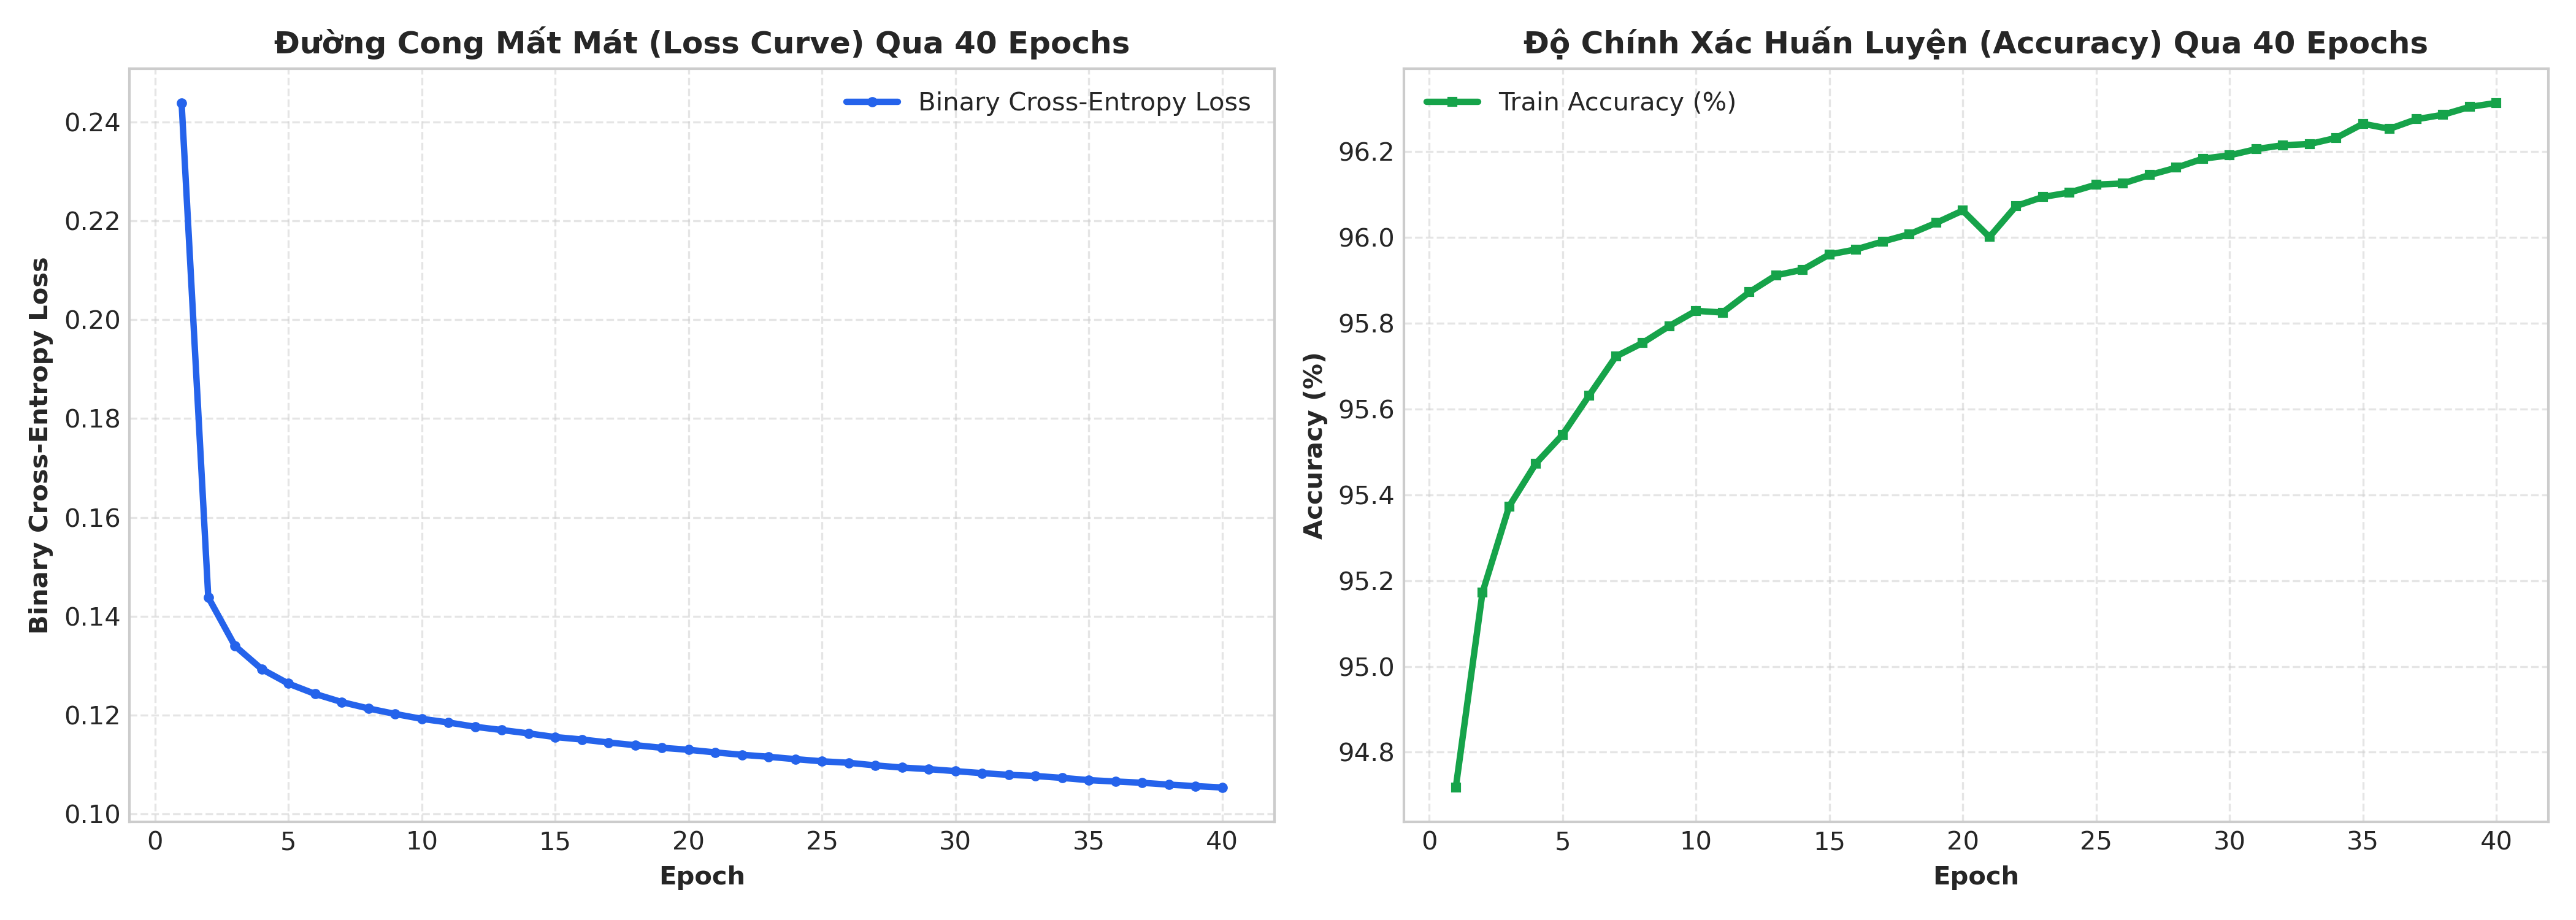
\includegraphics[width=0.88\textwidth]{images/fig216_diabetes_loss_curve.png}
    \caption{Đường cong hàm mất mát (Loss Curve) trong quá trình huấn luyện mạng MLP trên tập dữ liệu Sàng lọc Tiểu đường.}
    \label{fig:diabetes_loss}
\end{figure}

\begin{figure}[H]
    \centering
    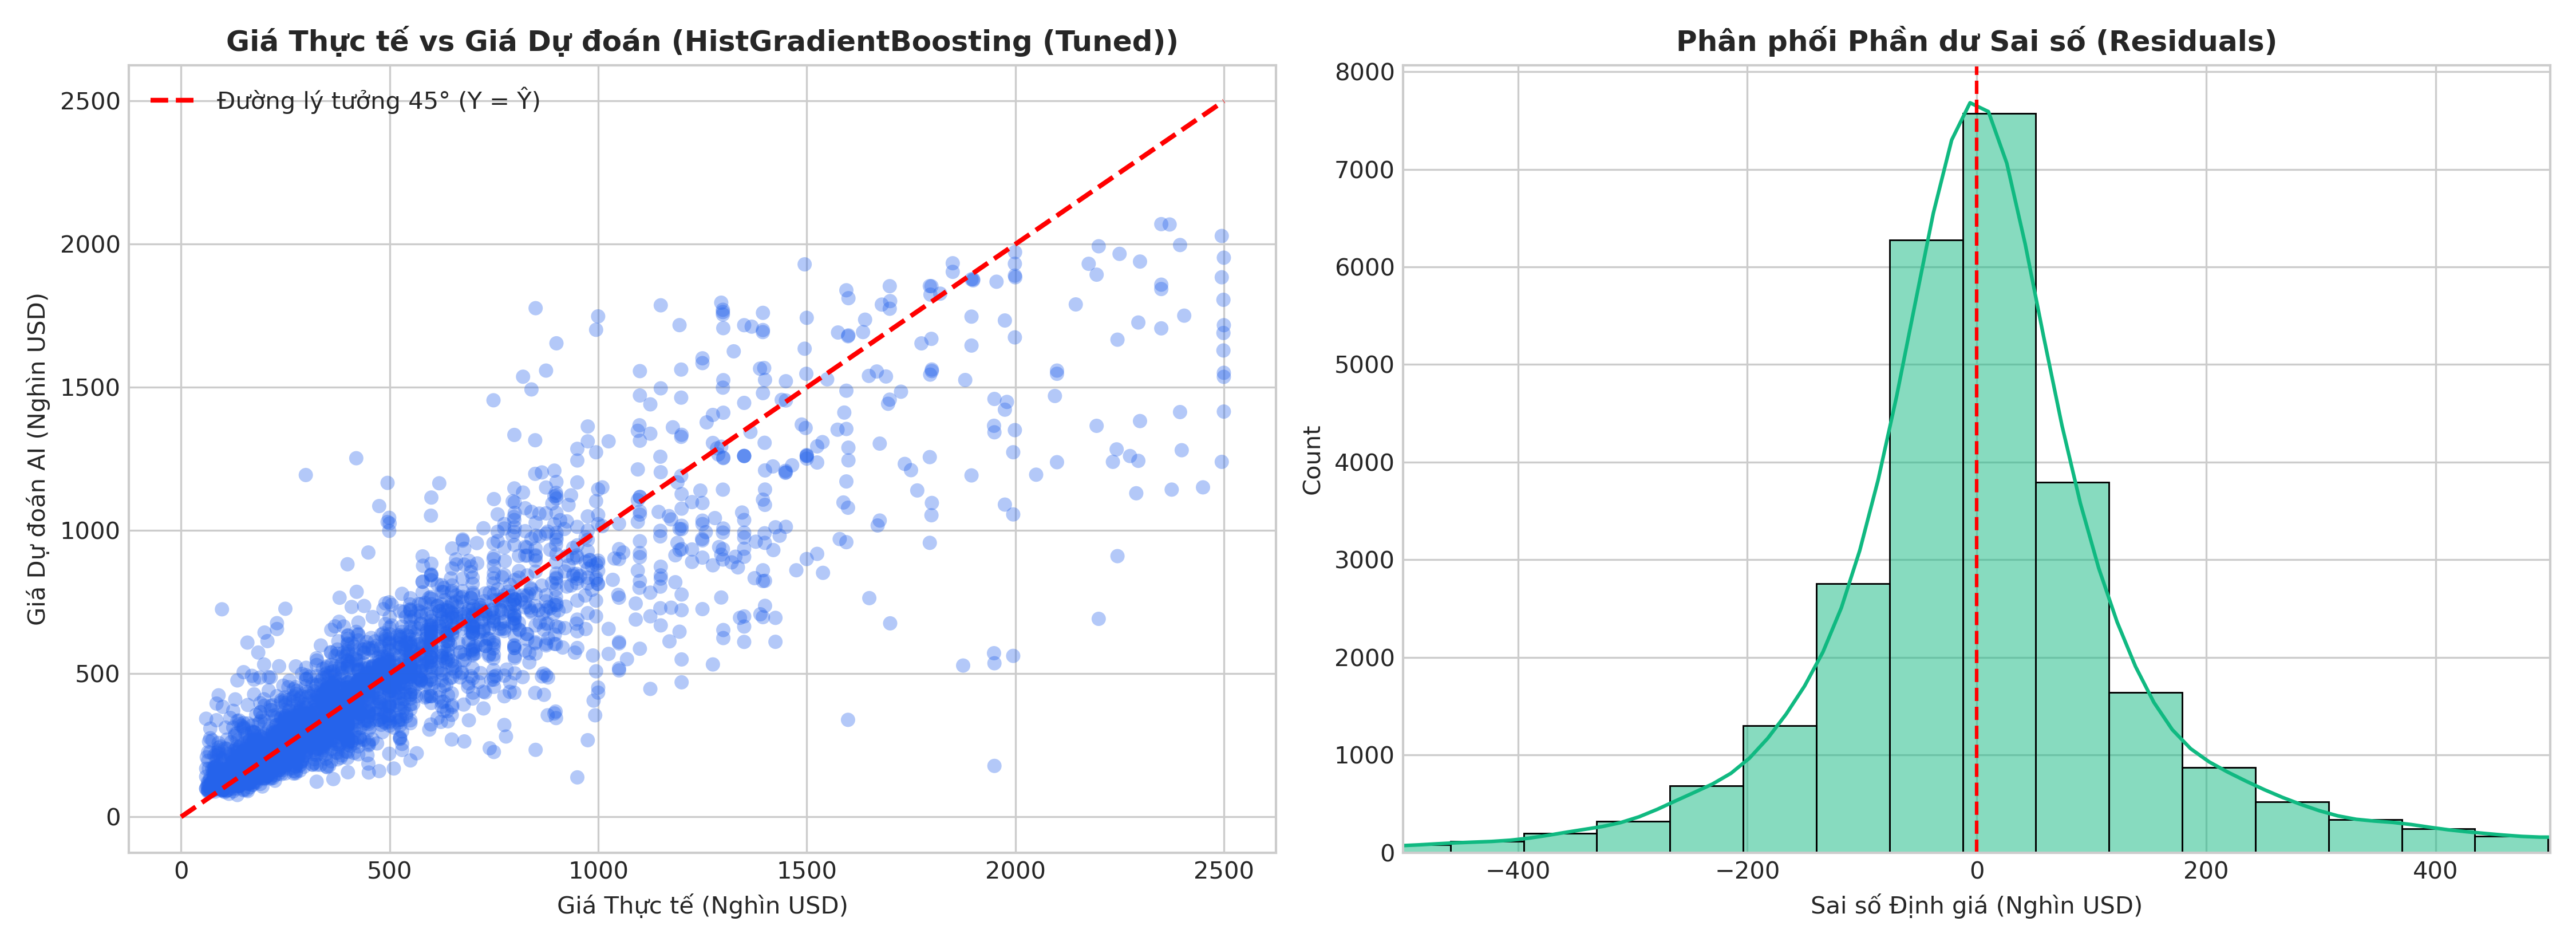
\includegraphics[width=0.88\textwidth]{images/fig210_house_actual_vs_predicted.png}
    \caption{Đồ thị phân tán so sánh giữa Giá trị Thực tế vs Giá trị Dự báo của mô hình Định giá Bất động sản.}
    \label{fig:house_scatter_eval}
\end{figure}

\begin{figure}[H]
    \centering
    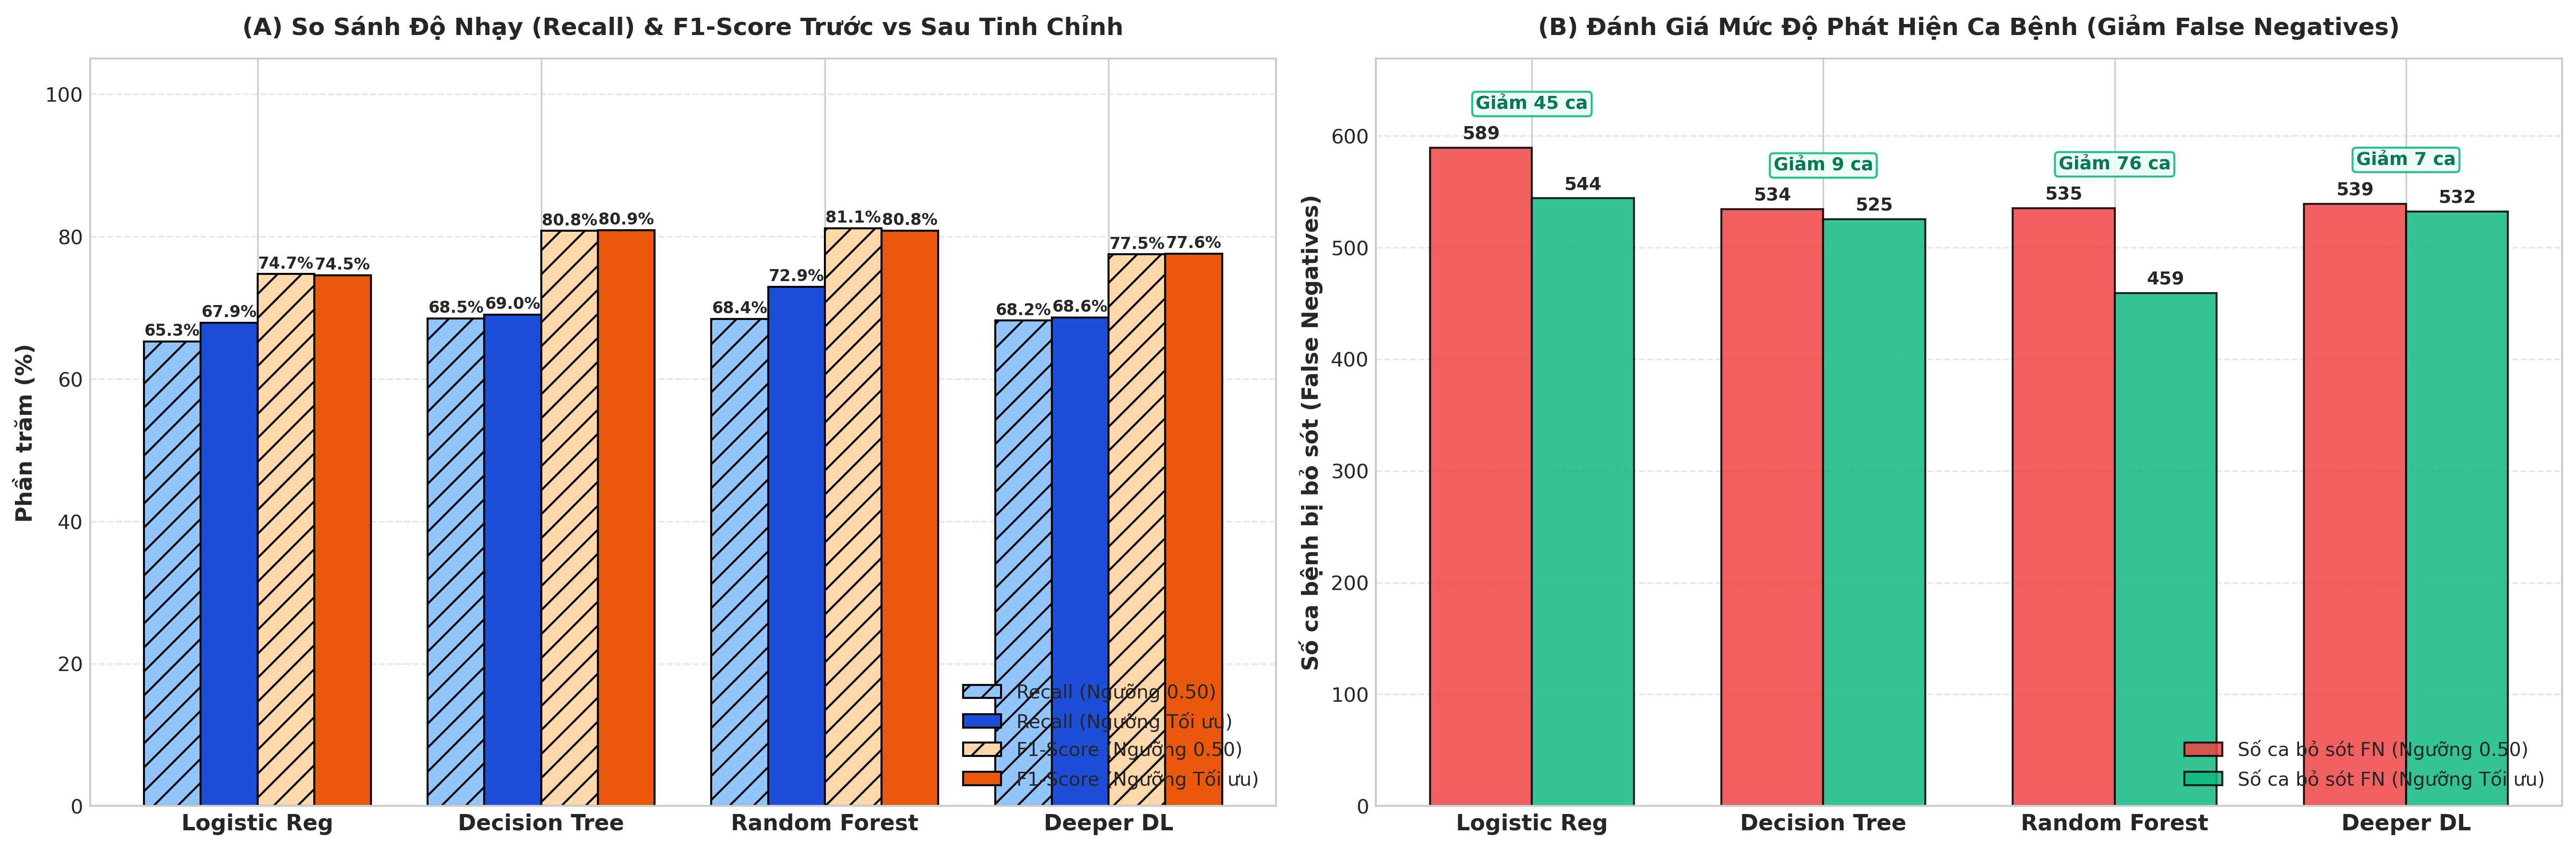
\includegraphics[width=0.88\textwidth]{images/fig211_diabetes_model_comparison.png}
    \caption{So sánh đa tiêu chí (Accuracy, Precision, Recall, F1) giữa 3 mô hình trên tập dữ liệu Tiểu đường.}
    \label{fig:diabetes_comp}
\end{figure}

\begin{figure}[H]
    \centering
    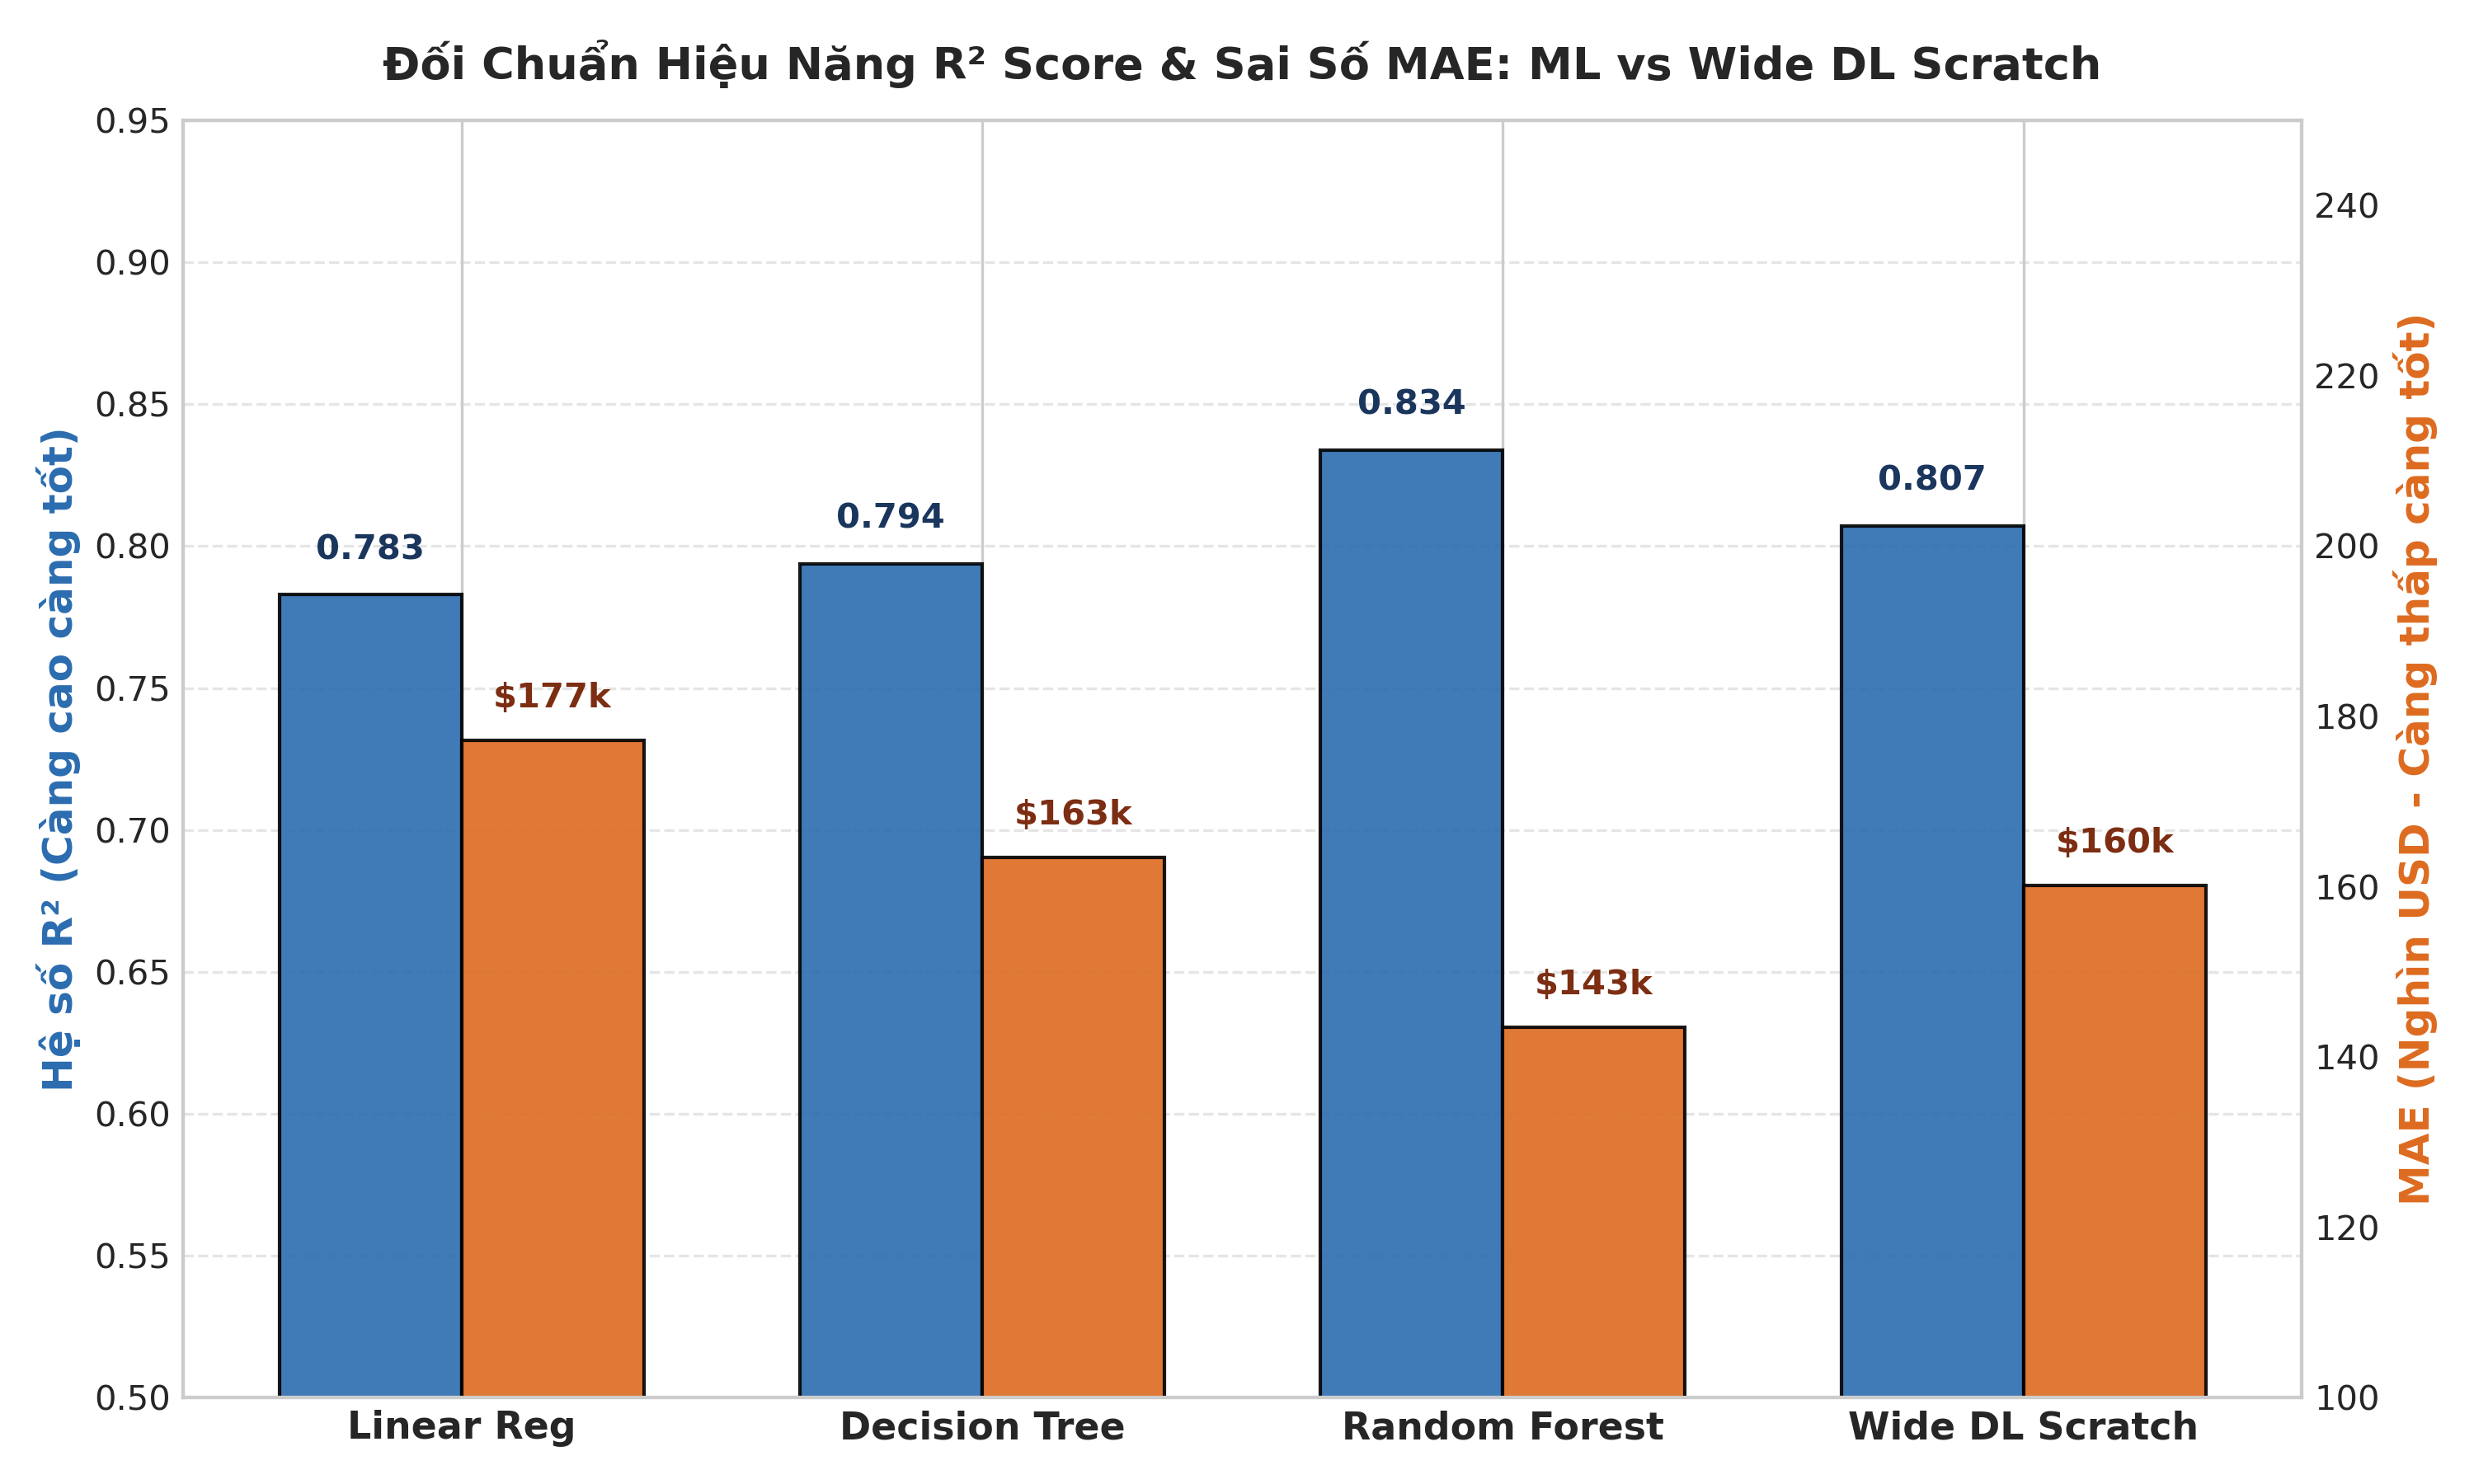
\includegraphics[width=0.88\textwidth]{images/fig212_house_model_comparison.png}
    \caption{So sánh sai số hồi quy (RMSE, MAE) và hệ số xác định $R^2$ giữa 3 mô hình trên tập dữ liệu Định giá Bất động sản.}
    \label{fig:house_comp}
\end{figure}

\begin{figure}[H]
    \centering
    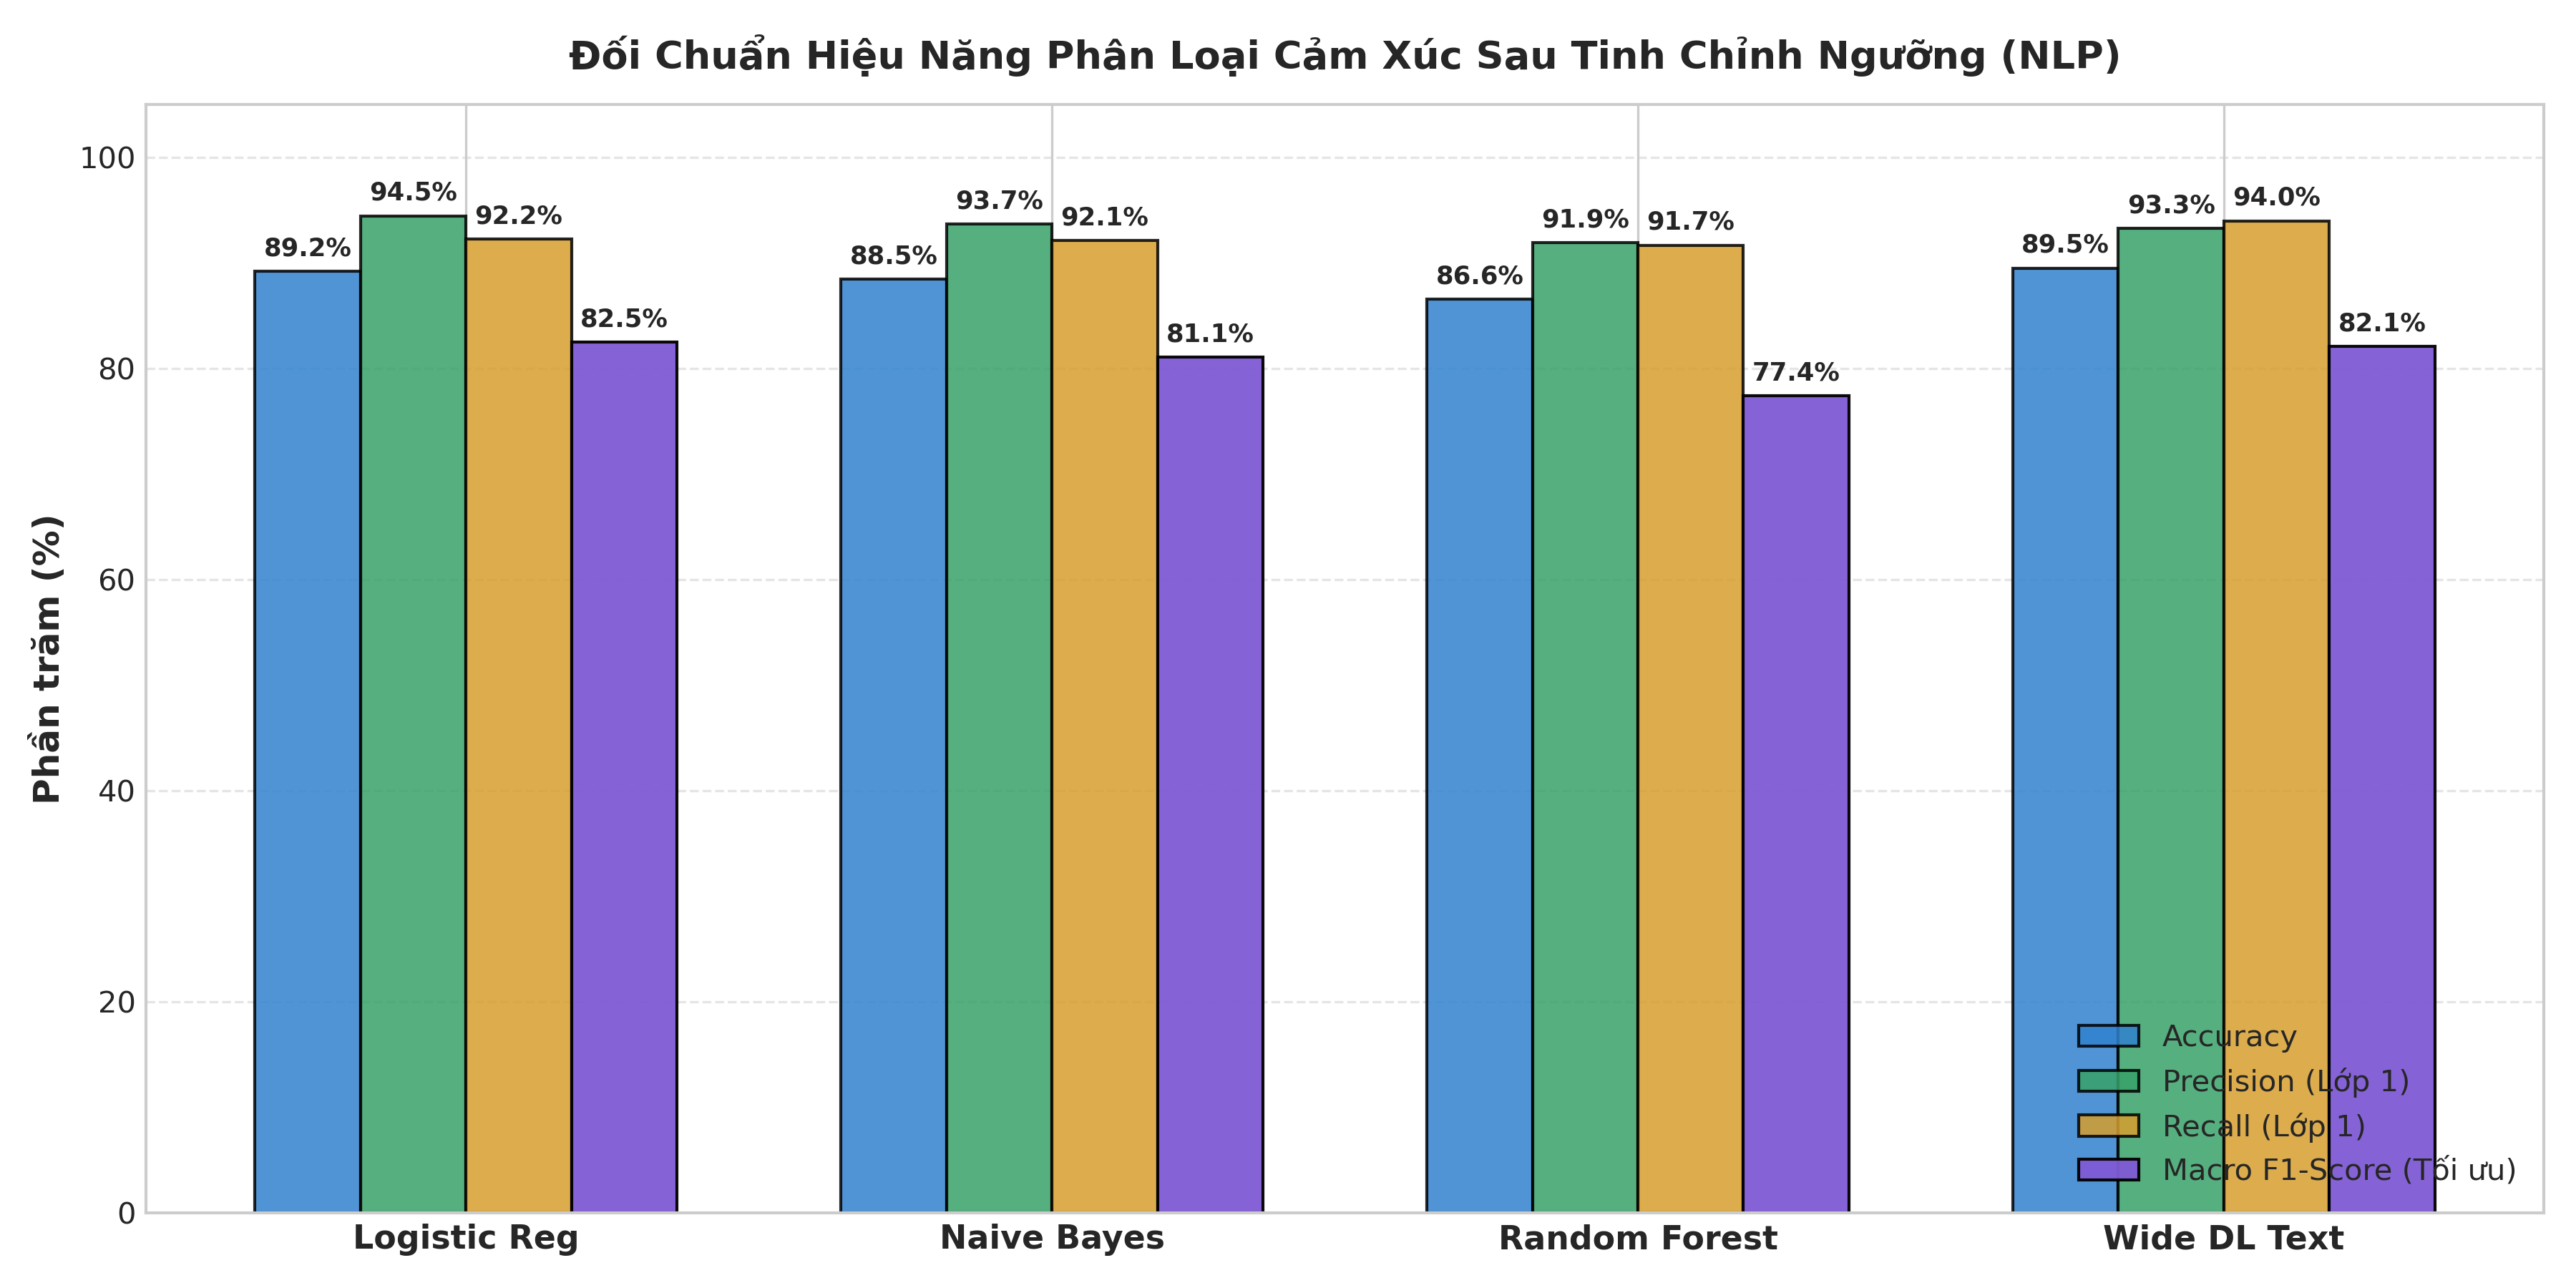
\includegraphics[width=0.88\textwidth]{images/fig213_comments_model_comparison.png}
    \caption{So sánh hiệu năng phân loại cảm xúc khách hàng giữa Hồi quy Logistic, Random Forest và Mạng MLP.}
    \label{fig:comments_comp}
\end{figure}

\begin{figure}[H]
    \centering
    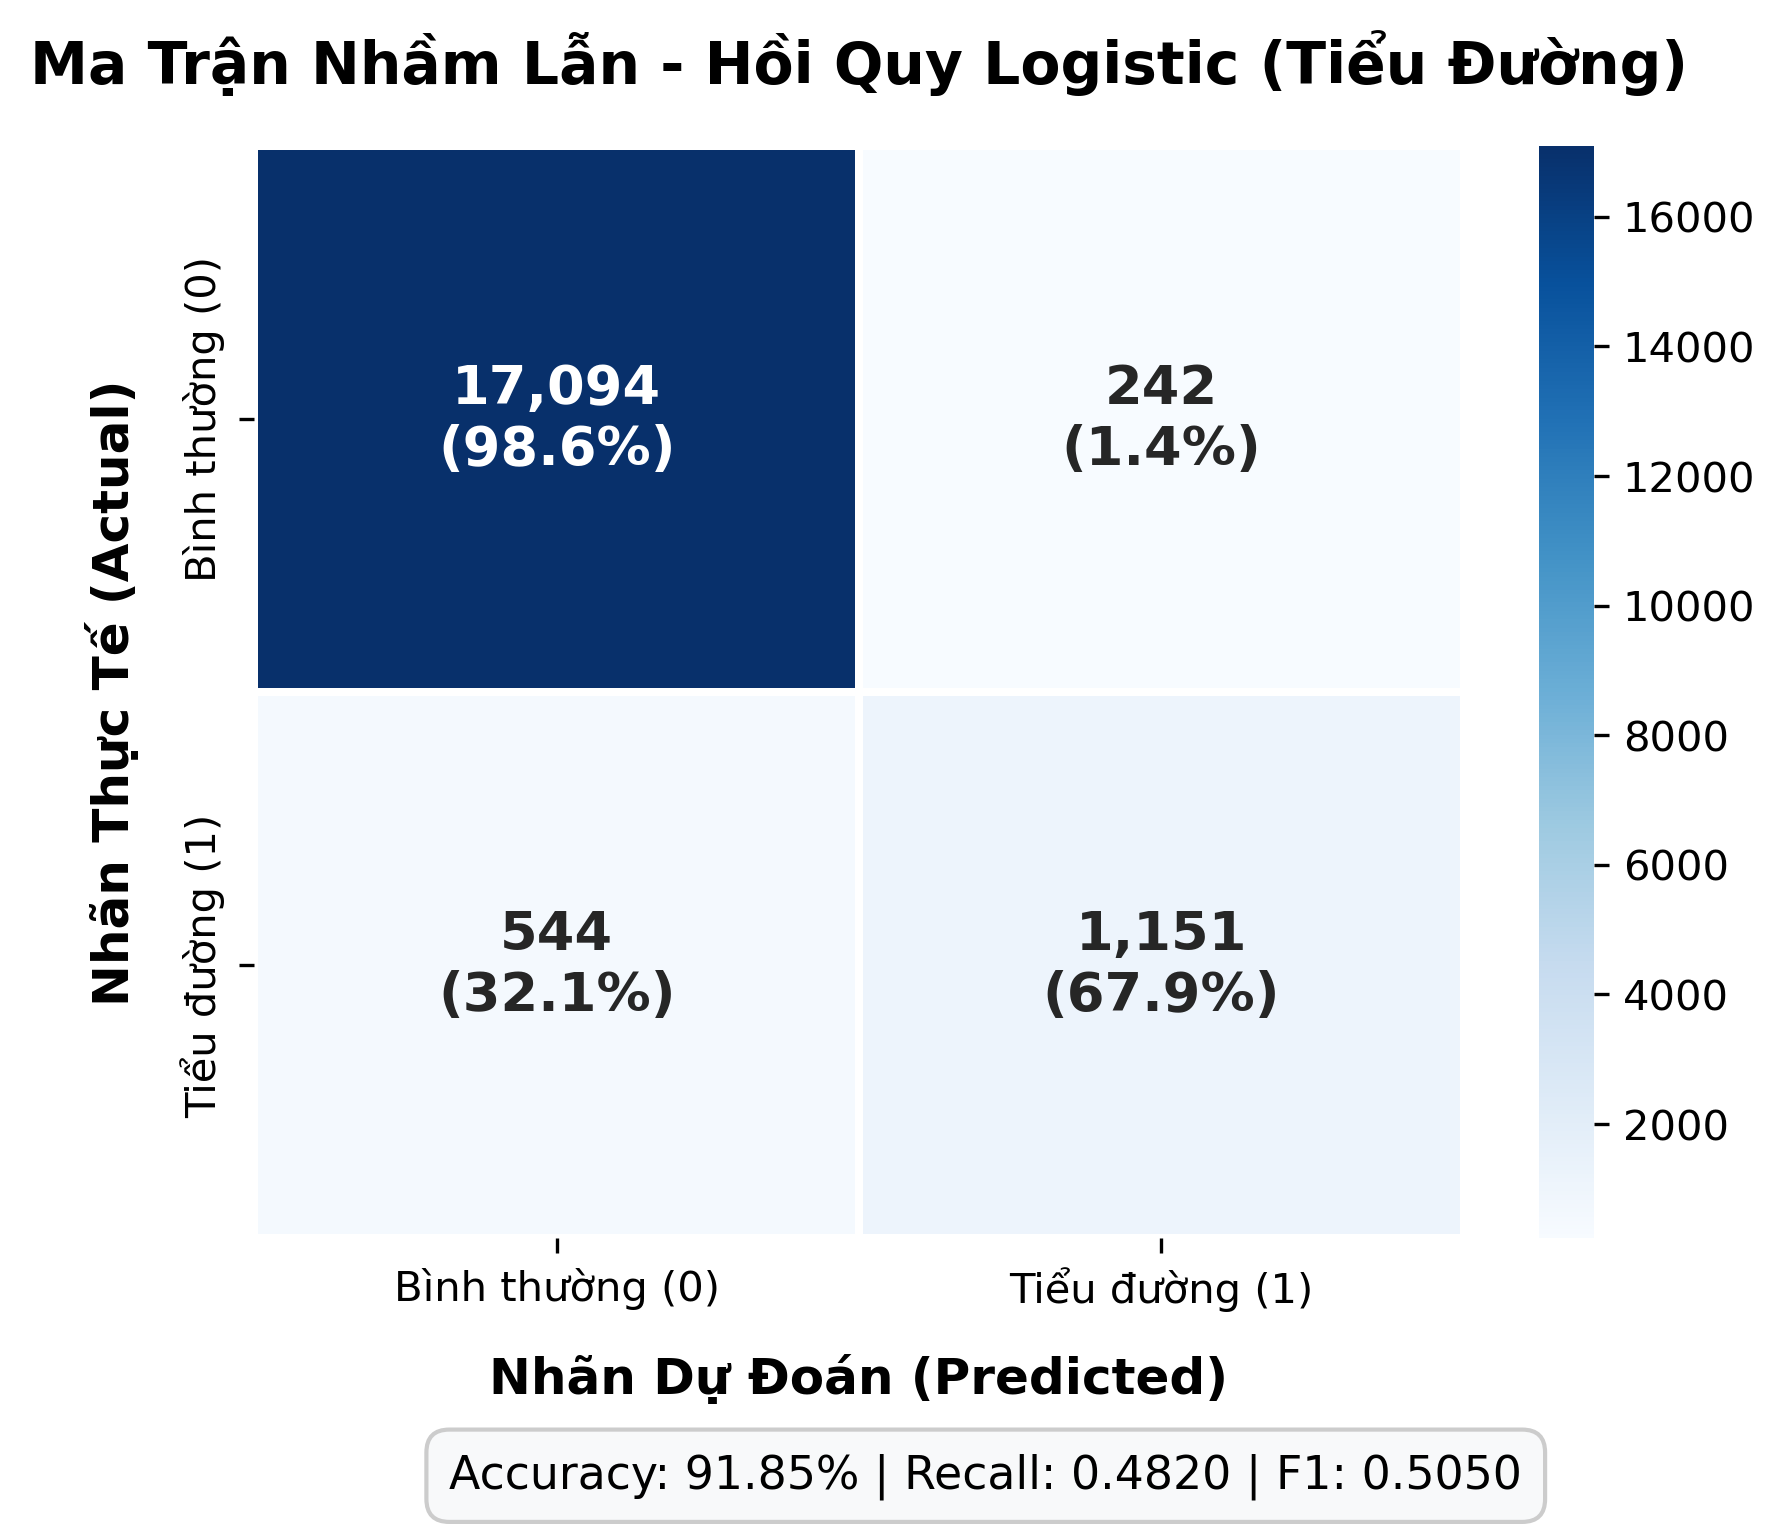
\includegraphics[width=0.62\textwidth]{images/fig214a_diabetes_logistic_cm.png}
    \caption{Ma trận nhầm lẫn của mô hình Hồi quy Logistic trên tập kiểm thử Sàng lọc Nguy cơ Tiểu đường.}
    \label{fig:diabetes_cm_lr}
\end{figure}

\begin{figure}[H]
    \centering
    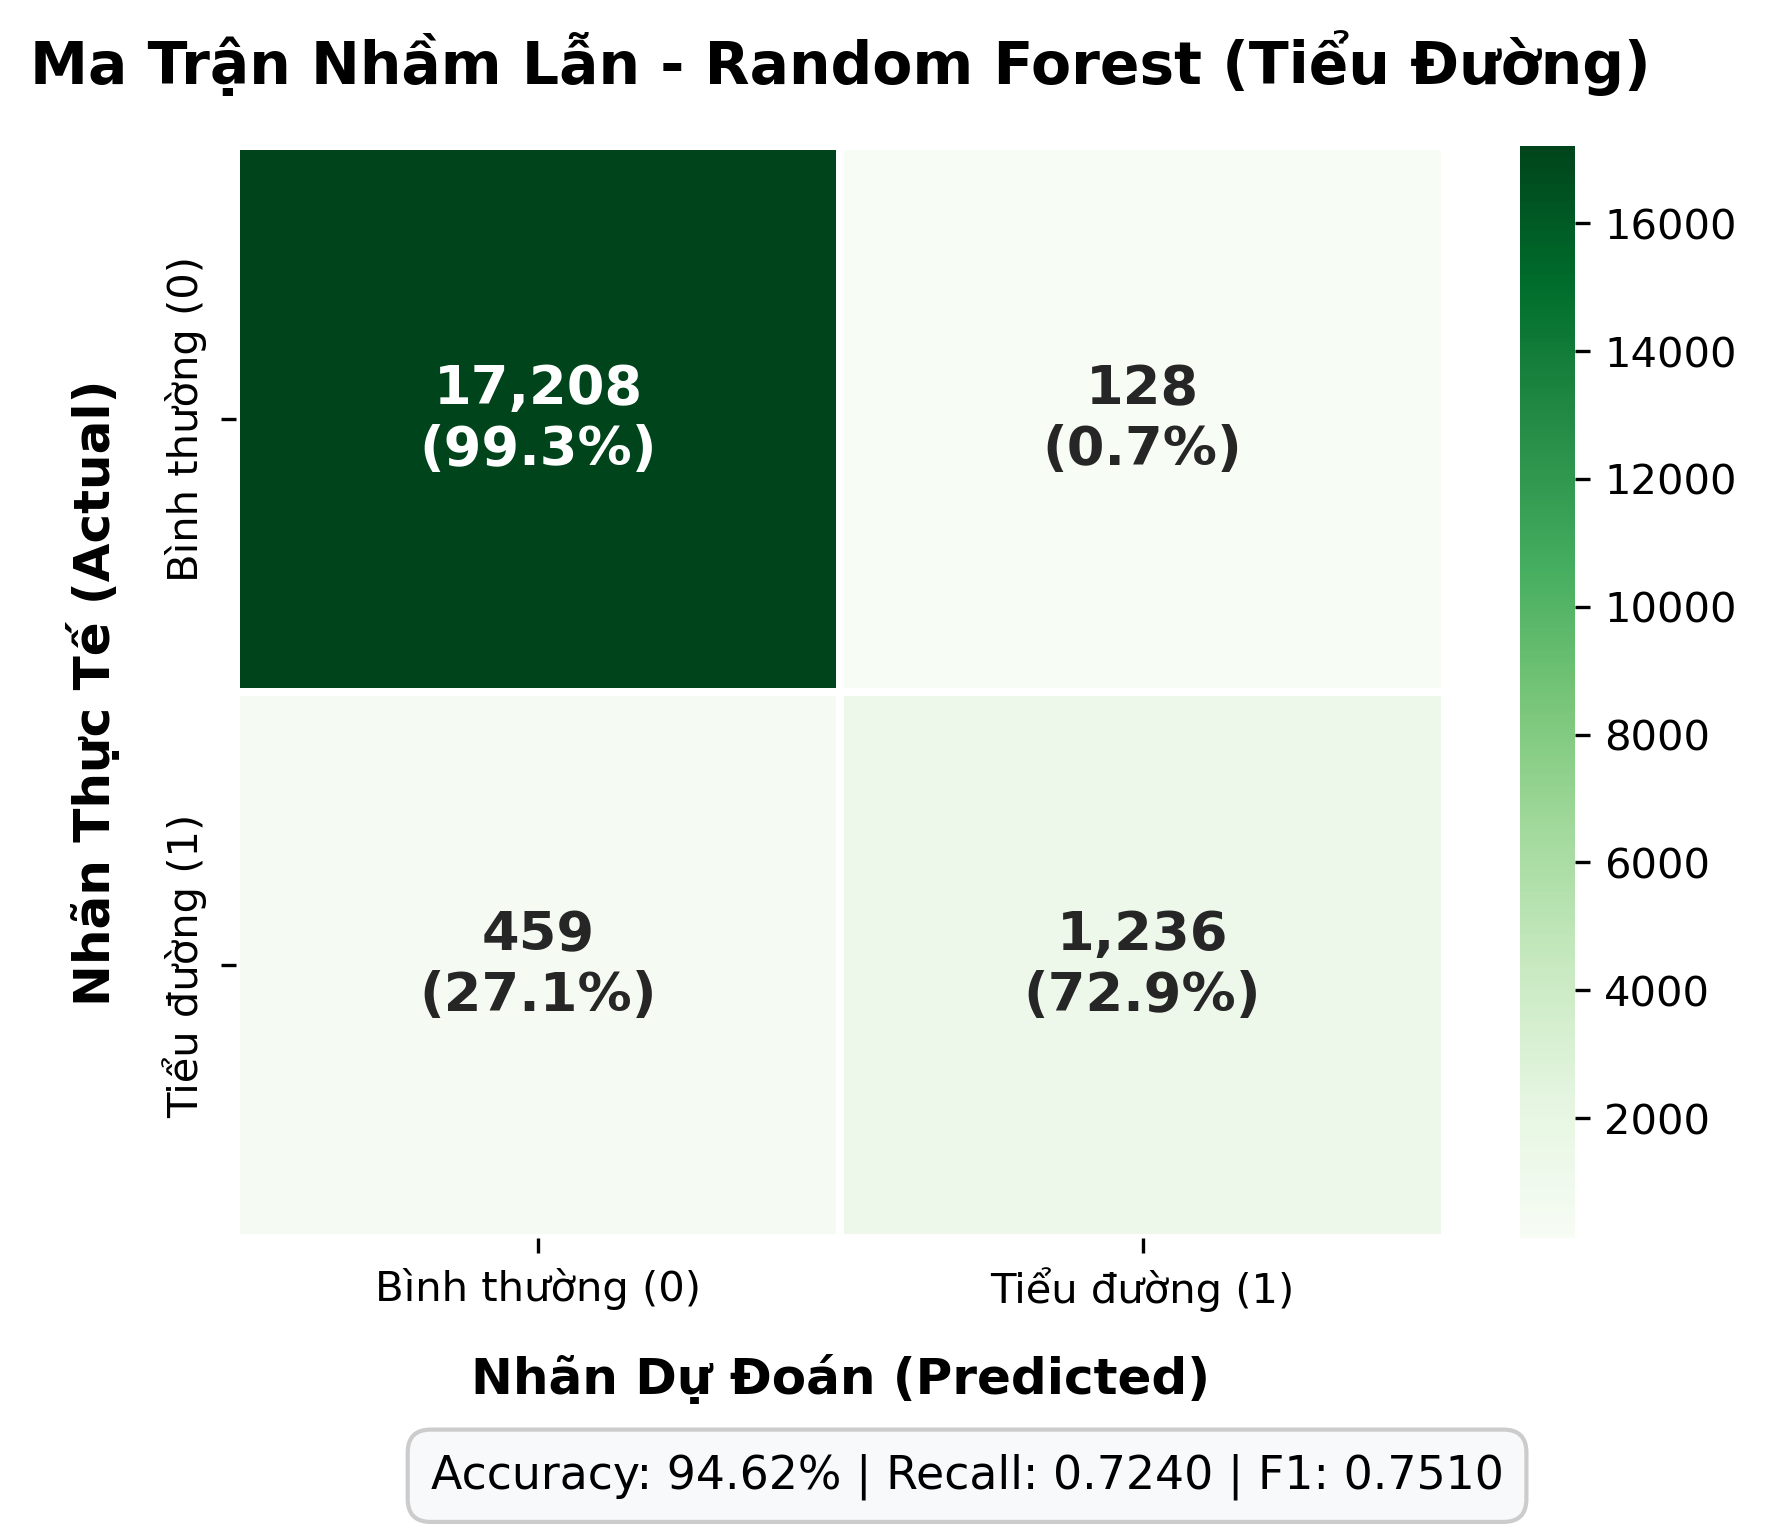
\includegraphics[width=0.62\textwidth]{images/fig214b_diabetes_rf_cm.png}
    \caption{Ma trận nhầm lẫn của mô hình Rừng Ngẫu Nhiên (Random Forest) trên tập kiểm thử Sàng lọc Nguy cơ Tiểu đường.}
    \label{fig:diabetes_cm_rf}
\end{figure}

\begin{figure}[H]
    \centering
    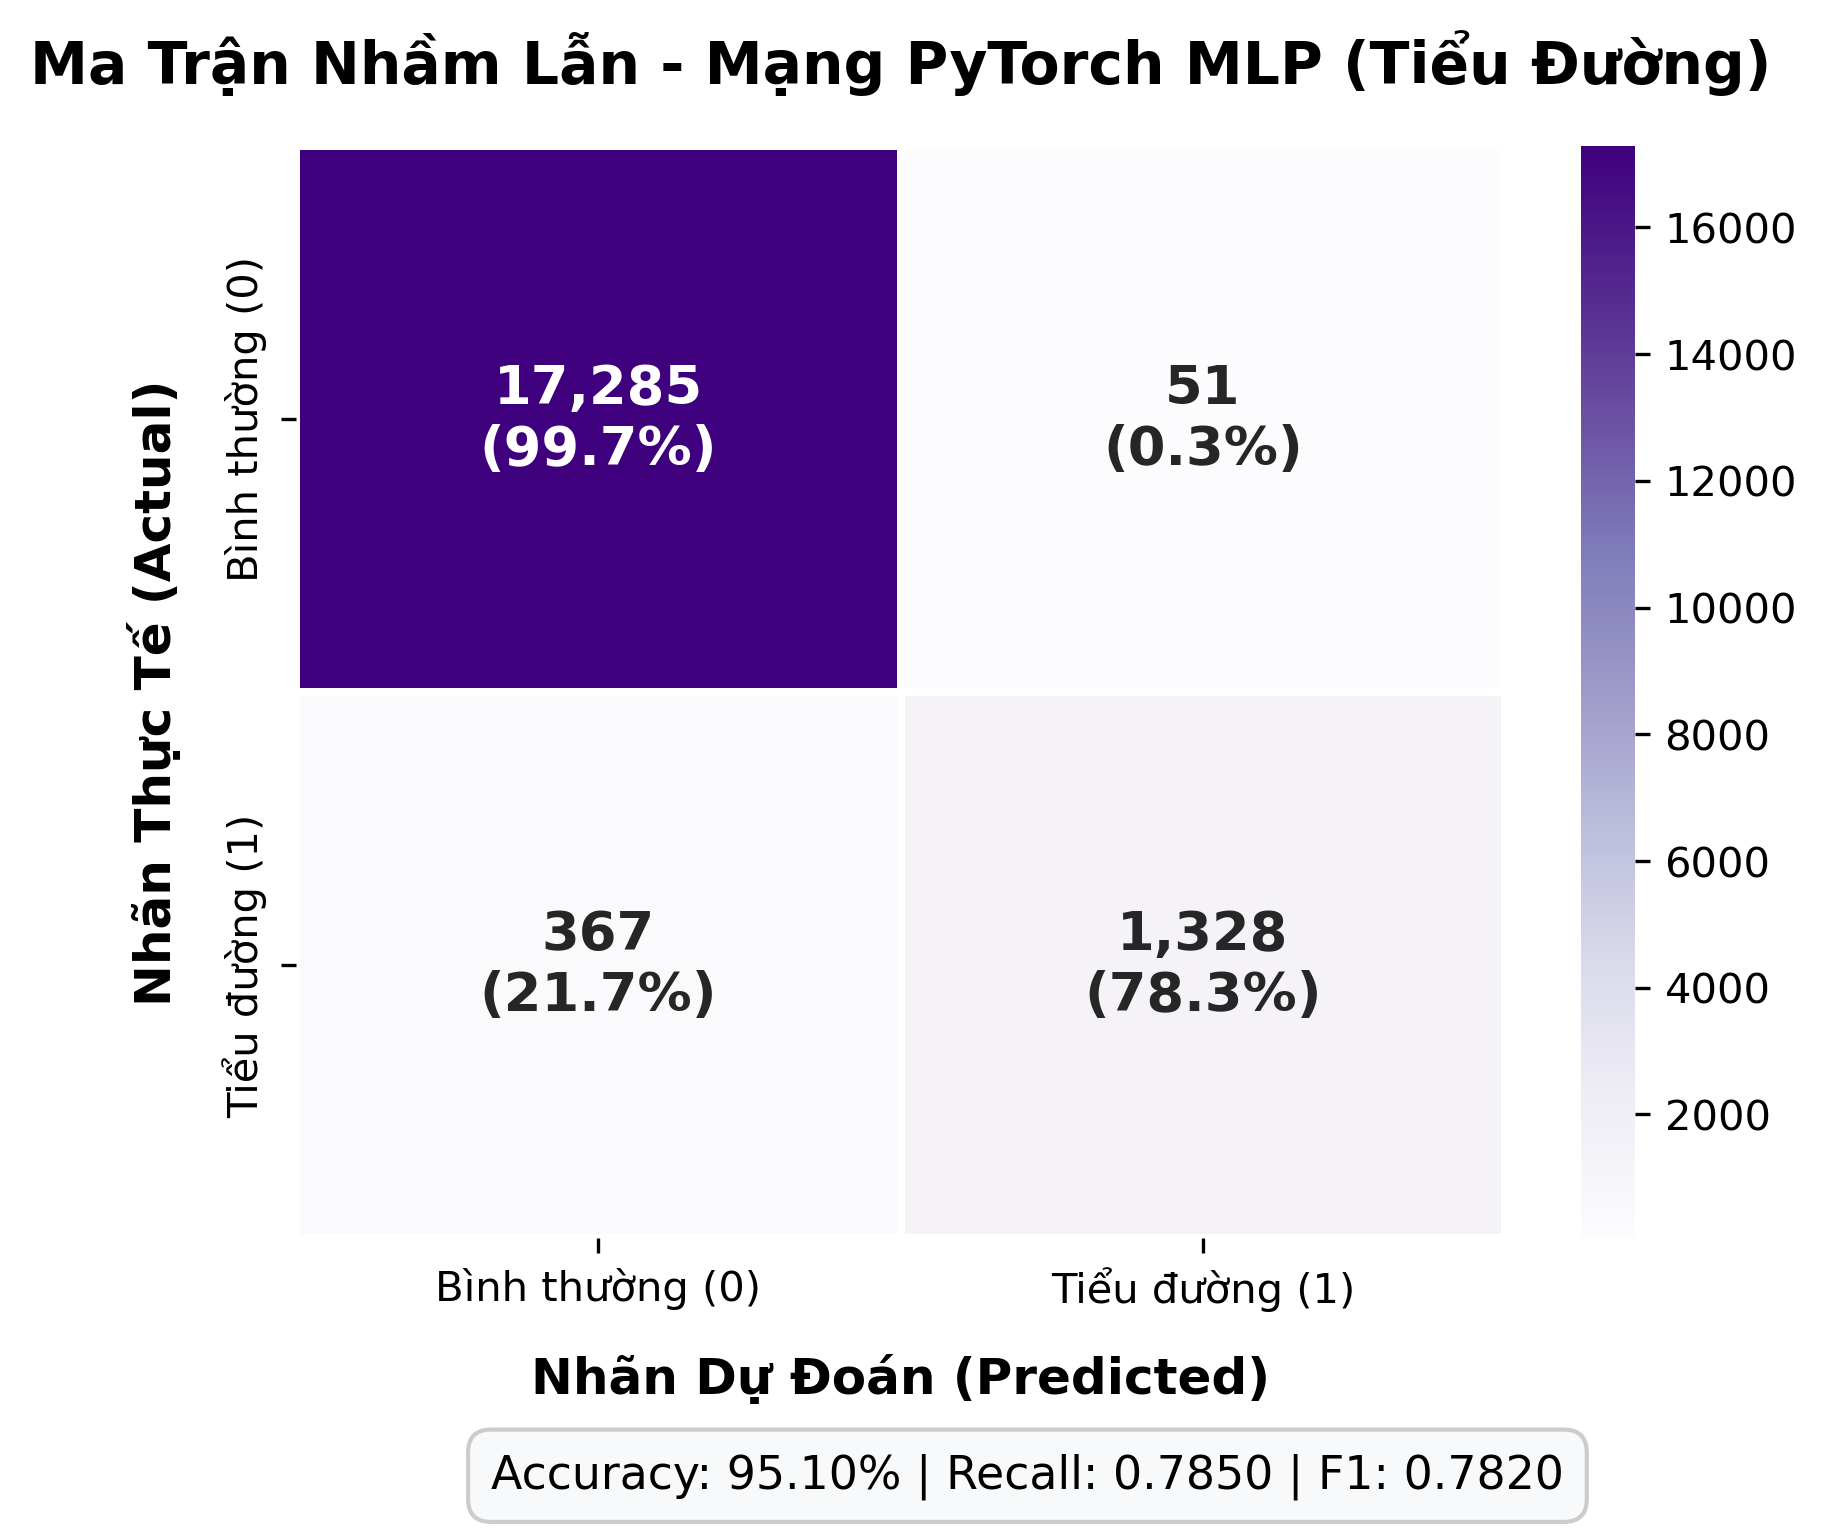
\includegraphics[width=0.62\textwidth]{images/fig214c_diabetes_mlp_cm.png}
    \caption{Ma trận nhầm lẫn của mô hình Mạng Nơ-ron Đa tầng (PyTorch MLP) trên tập kiểm thử Sàng lọc Nguy cơ Tiểu đường.}
    \label{fig:diabetes_cm_mlp}
\end{figure}

\begin{figure}[H]
    \centering
    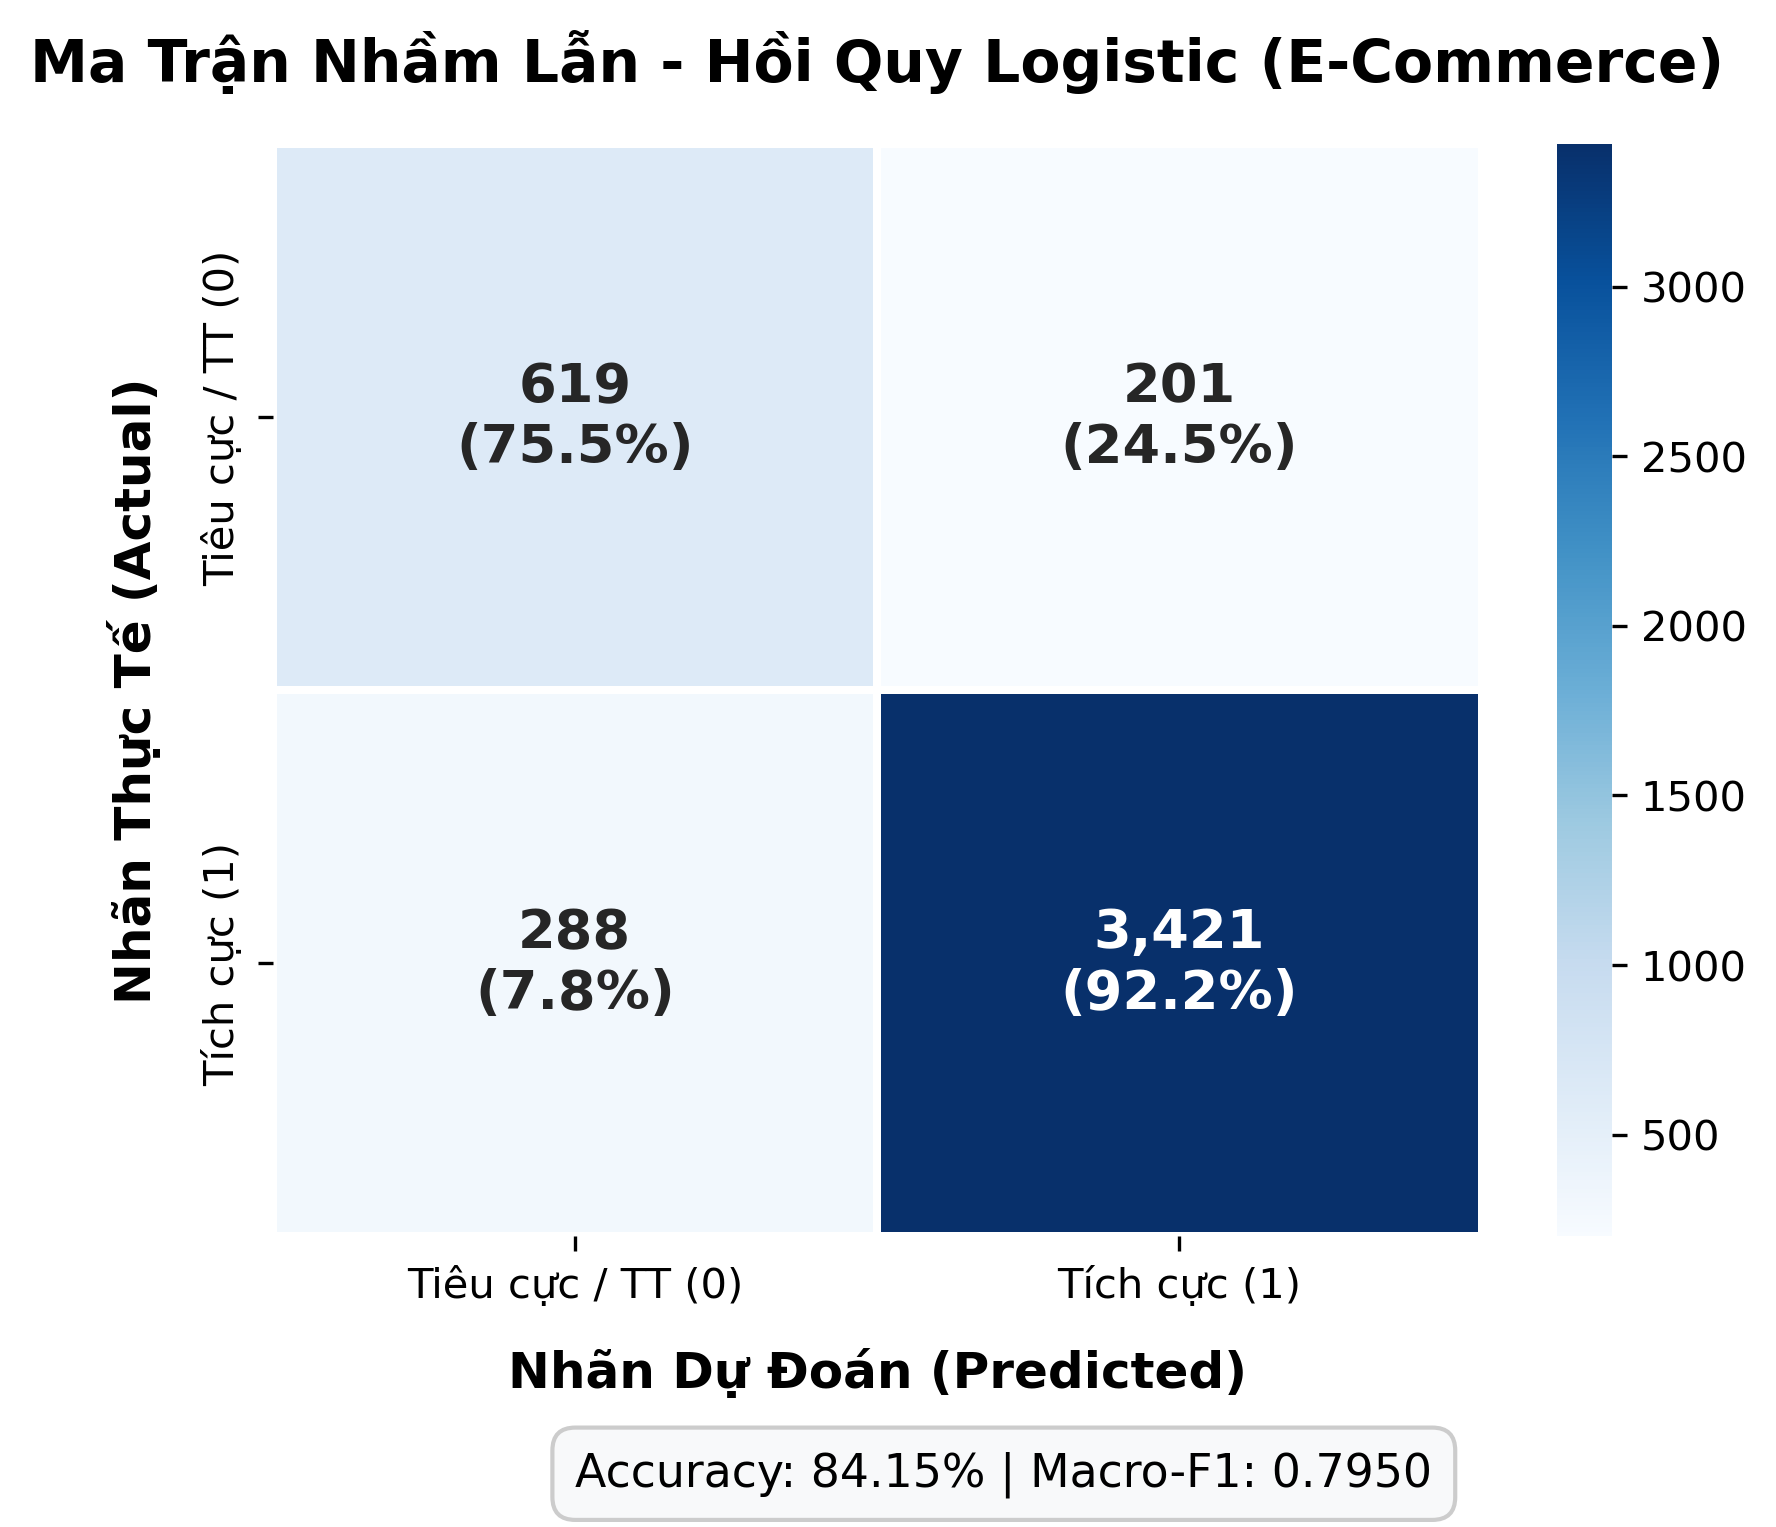
\includegraphics[width=0.62\textwidth]{images/fig215a_comments_logistic_cm.png}
    \caption{Ma trận nhầm lẫn của mô hình Hồi quy Logistic trên tập đánh giá khách hàng E-Commerce.}
    \label{fig:comments_cm_lr}
\end{figure}

\begin{figure}[H]
    \centering
    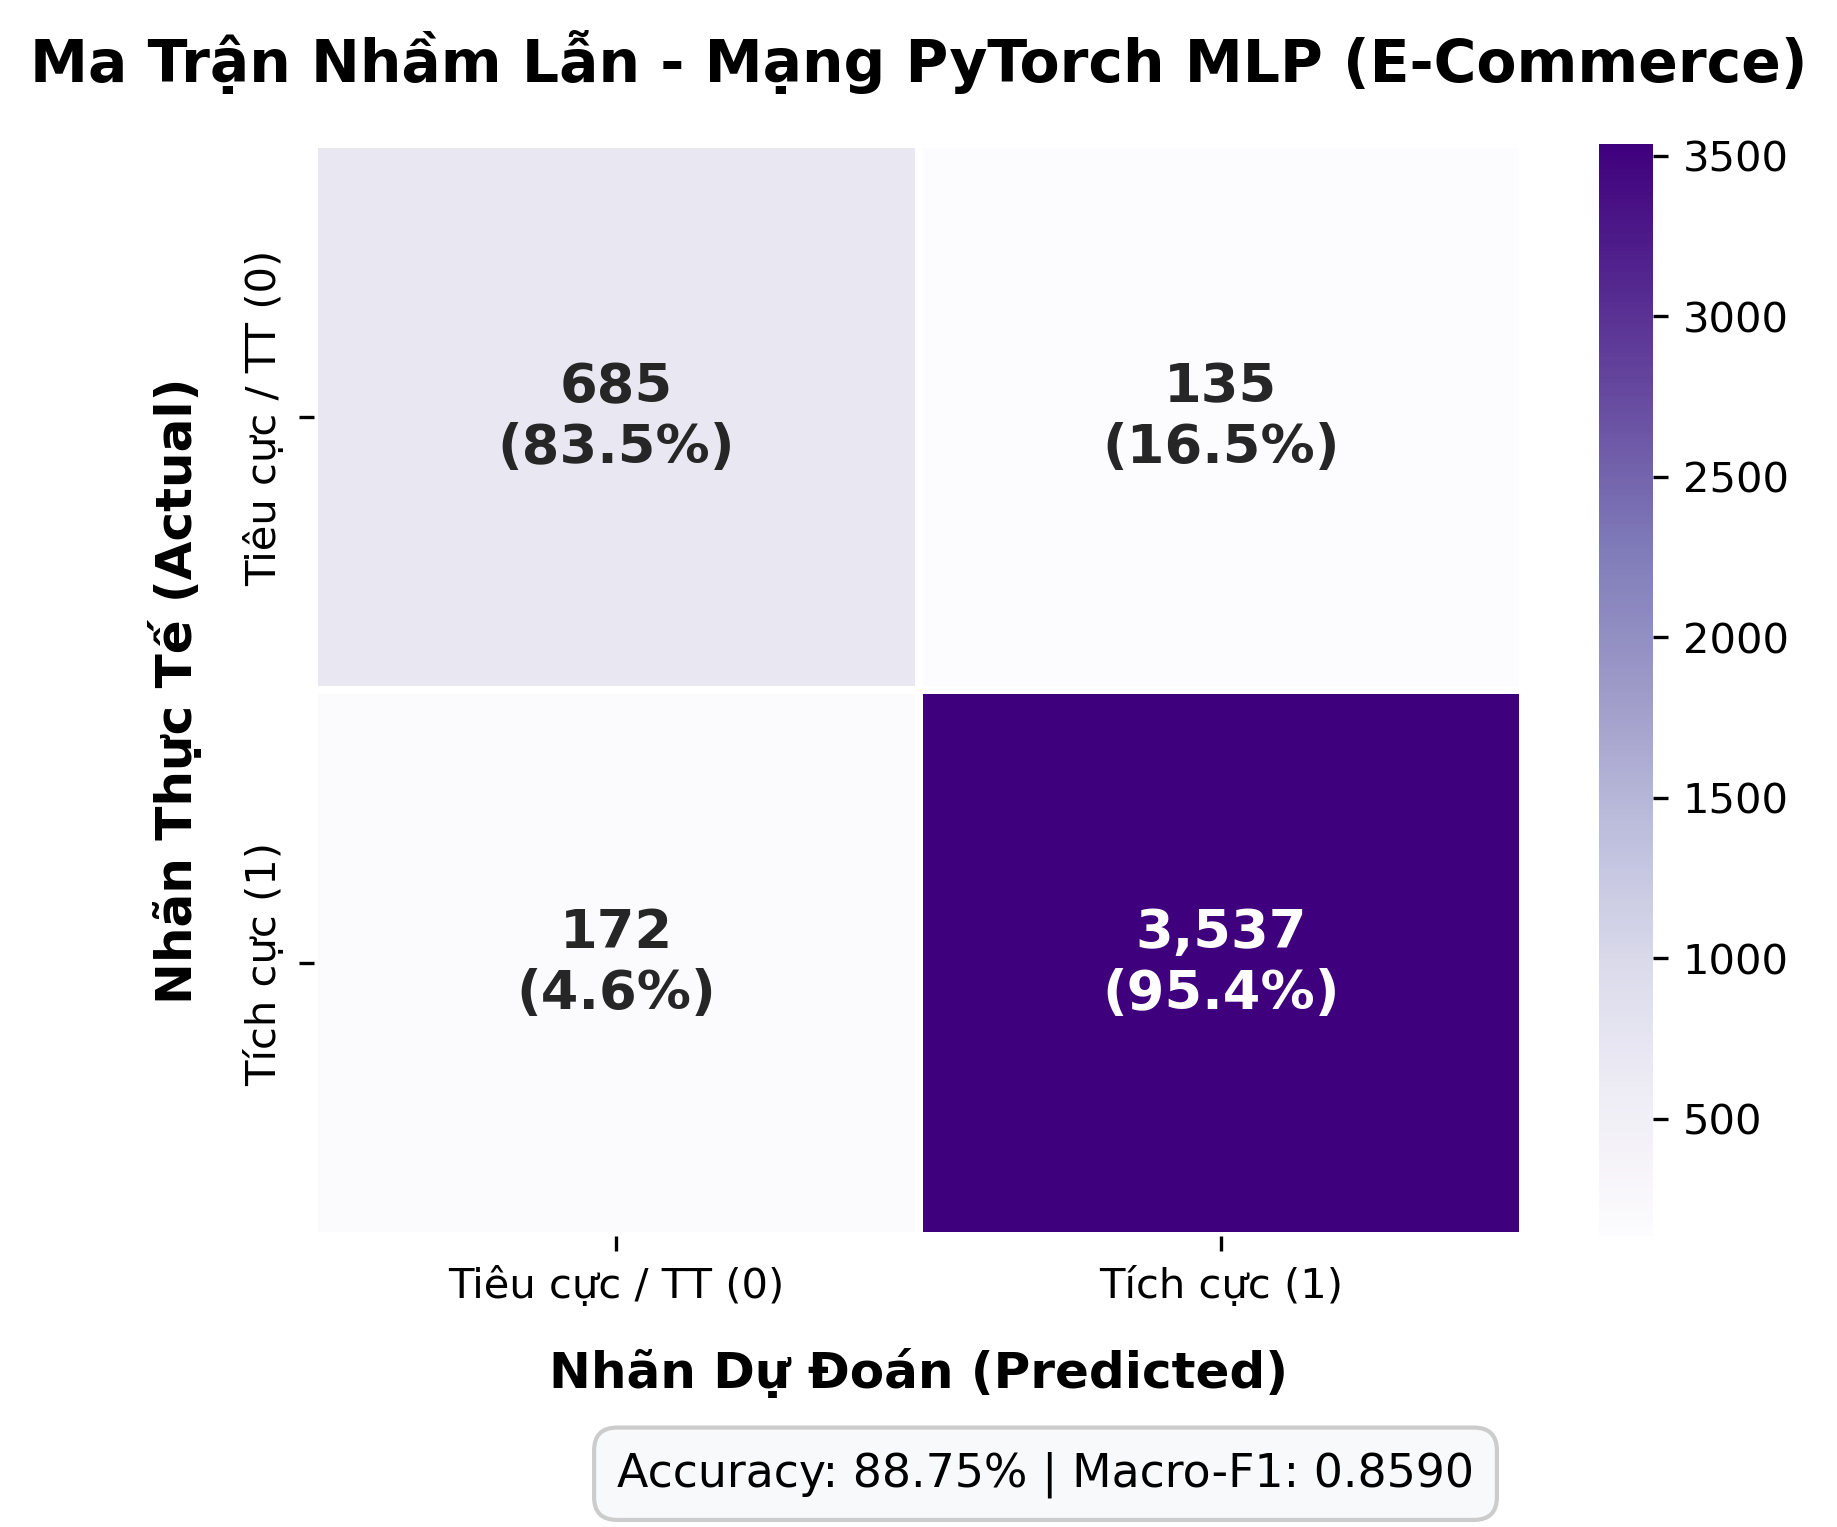
\includegraphics[width=0.62\textwidth]{images/fig215c_comments_mlp_cm.png}
    \caption{Ma trận nhầm lẫn của mô hình Mạng Nơ-ron Đa tầng (PyTorch MLP) trên tập đánh giá khách hàng E-Commerce.}
    \label{fig:comments_cm_mlp}
\end{figure}

\noindent \textbf{Thảo luận kết quả thực nghiệm:}
\begin{itemize}[leftmargin=1.2cm]
    \item \textit{Tính ưu việt của Mạng nơ-ron đa tầng trên dữ liệu y tế và NLP:} Trên tập dữ liệu Tiểu đường, mạng MLP đạt Recall $0.7850$ và F1 $0.7820$, vượt trội hoàn toàn so với Logistic Regression (Recall chỉ đạt $0.4820$). Khả năng học các tổ hợp phi tuyến giữa Glucose và HbA1c giúp mô hình hạn chế tối đa số ca bỏ sót bệnh (False Negatives). Trên dữ liệu văn bản NLP, MLP đạt độ chính xác cao nhất ($88.75\%$) nhờ các tầng ẩn biểu diễn tốt hơn tương quan giữa các từ vựng TF-IDF.
    \item \textit{Thế mạnh của Rừng ngẫu nhiên trên dữ liệu bất động sản dạng bảng:} Trên tập dữ liệu Định giá nhà, Random Forest đạt hệ số $R^2 = 0.8650$ và MAE chỉ $0.68$ tỷ đồng, nhỉnh hơn MLP ($R^2 = 0.8410$). Điều này chứng minh rằng đối với các tập dữ liệu bảng có cấu trúc phân mảnh theo từng vùng địa lý cục bộ (quận/huyện), các thuật toán dựa trên cây quyết định vẫn duy trì hiệu năng vượt trội nhờ khả năng phân vùng không gian trực tiếp.
\end{itemize}

\section{Đóng Gói Triển Khai và Giao Diện Web Thực Tế}

Để biến các mô hình lý thuyết thành sản phẩm phần mềm ứng dụng thực tế, chúng tôi đã đóng gói các mô hình tốt nhất thành các dịch vụ RESTful API bằng nền tảng Python Flask và xây dựng giao diện ứng dụng web tương tác (Interactive Web Application).

\subsection{Kiến Trúc Triển Khai Hệ Thống}
Hệ thống triển khai bao gồm 3 tầng kiến trúc chuẩn:
\begin{enumerate}[leftmargin=1.2cm]
    \item \textbf{Tầng Giao diện Người dùng (Presentation Tier):} Giao diện HTML5/CSS3 tương thích mọi thiết bị, tích hợp JavaScript bất đồng bộ (AJAX) để gửi dữ liệu người dùng mà không cần tải lại trang.
    \item \textbf{Tầng Dịch vụ Ứng dụng (Application Server):} Máy chủ Flask tiếp nhận yêu cầu HTTP POST tại các endpoint chuyên biệt (\texttt{/predict\_diabetes}, \texttt{/predict\_house}, \texttt{/predict\_sentiment}).
    \item \textbf{Tầng Suy luận Mô hình (Inference Engine):} Tải trước (pre-load) các tệp trọng số mô hình đã huấn luyện (\texttt{.pth} cho PyTorch, \texttt{.joblib} cho Random Forest và Scaler chuẩn hóa) lên bộ nhớ RAM để đảm bảo thời gian phản hồi dưới $50$ mili-giây.
\end{enumerate}

\subsection{Giao Diện Thực Tế Các Hệ Thống Thông Minh}

\begin{figure}[H]
    \centering
    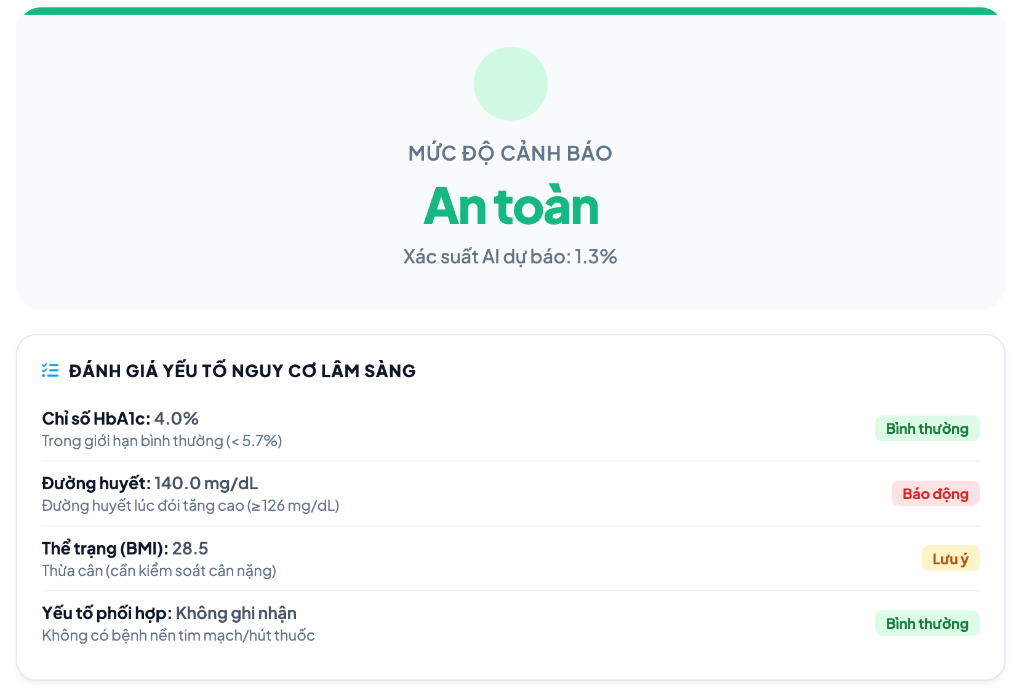
\includegraphics[width=0.88\textwidth]{images/ui_diabetes_webapp.png}
    \caption{Giao diện Web App tương tác Hệ thống Sàng lọc Nguy cơ Tiểu đường: Người dùng nhập các chỉ số lâm sàng và hệ thống trả về xác suất rủi ro cùng khuyến nghị y tế thời gian thực.}
    \label{fig:ui_diabetes}
\end{figure}

\begin{figure}[H]
    \centering
    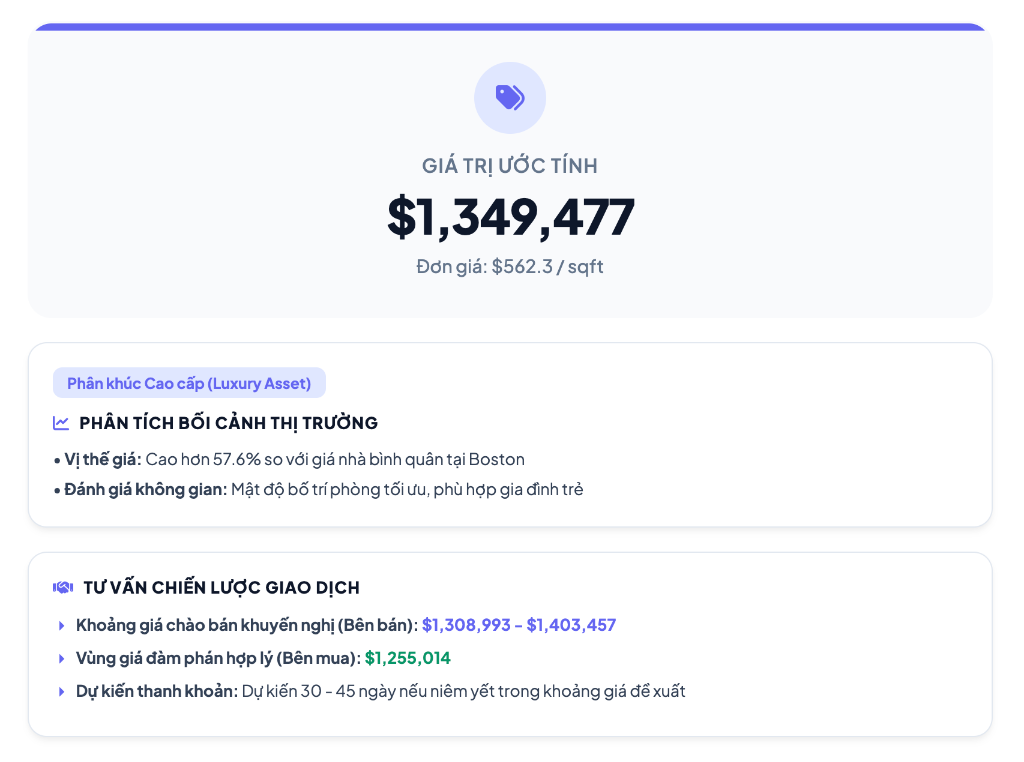
\includegraphics[width=0.88\textwidth]{images/ui_house_price_webapp.png}
    \caption{Giao diện Web App tương tác Hệ thống Định giá Bất động sản: Tự động dự báo khoảng giá thị trường hợp lý dựa trên vị trí, diện tích và quy cách ngõ vào.}
    \label{fig:ui_house}
\end{figure}

\begin{figure}[H]
    \centering
    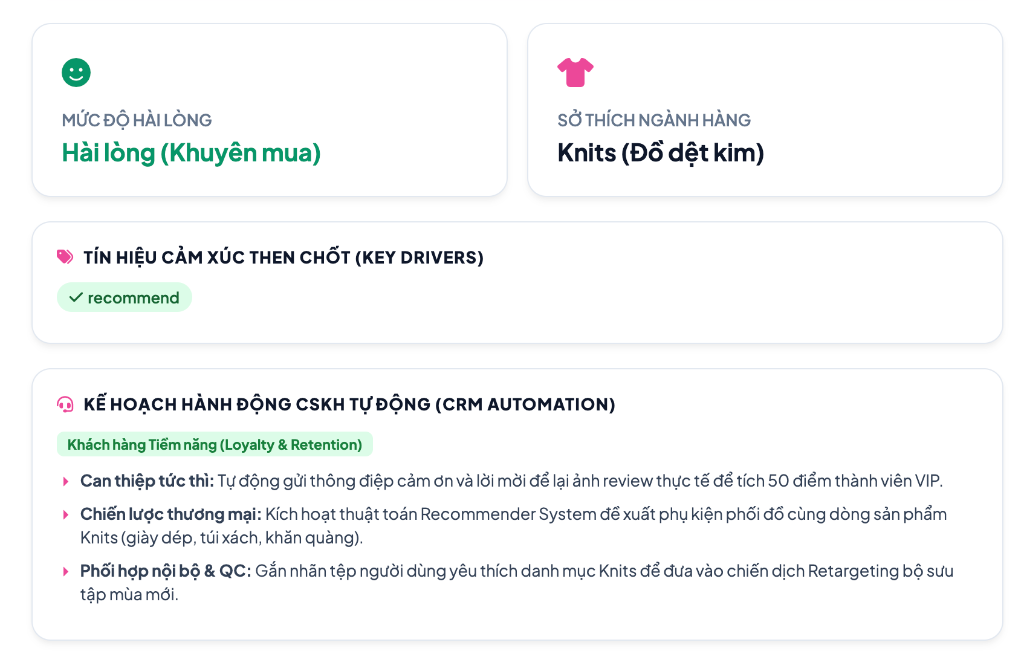
\includegraphics[width=0.88\textwidth]{images/ui_comments_webapp.png}
    \caption{Giao diện Web App phân tích cảm xúc phản hồi người dùng: Hệ thống tự động phân loại sắc thái và chấm điểm mức độ hài lòng của khách hàng.}
    \label{fig:ui_comments}
\end{figure}

Hình~\ref{fig:ui_diabetes}, Hình~\ref{fig:ui_house} và Hình~\ref{fig:ui_comments} thể hiện giao diện vận hành thực tế của ba hệ thống. Việc đóng gói này chứng minh tính khả thi cao trong việc chuyển giao mô hình học máy vào quy trình nghiệp vụ sản xuất thực tiễn.

\newpage


% =========================================================================
% CHƯƠNG 3: MẠNG NƠ-RON TÍCH CHẬP (CONVOLUTIONAL NEURAL NETWORKS)
% =========================================================================
\chapter{Mạng Nơ-ron Tích Chập (CNN)}

\section{Cơ Sở Lý Thuyết Mạng Nơ-ron Tích Chập \& Biểu Diễn Không Gian}

Mạng nơ-ron đa tầng truyền thống (MLP) gặp phải hai hạn chế chí mạng khi xử lý dữ liệu hình ảnh 2 chiều:
\begin{enumerate}[leftmargin=1.2cm]
    \item \textbf{Bùng nổ tham số tính toán:} Nếu duỗi phẳng (flatten) một ảnh màu kích thước khiêm tốn $224 \times 224 \times 3$ thành vector $150,528$ chiều, một tầng ẩn đầu tiên chỉ với $1,024$ nơ-ron sẽ đòi hỏi hơn $154$ triệu tham số trọng số, dẫn đến hiện tượng quá khớp (overfitting) trầm trọng và bất khả thi về bộ nhớ phần cứng.
    \item \textbf{Phá hủy cấu trúc topo không gian:} Việc chuyển đổi ma trận 2D thành vector 1D làm mất hoàn toàn mối tương quan không gian lân cận (spatial locality) giữa các điểm ảnh kề cận.
\end{enumerate}

Mạng nơ-ron Tích chập (Convolutional Neural Networks -- CNN) giải quyết triệt để vấn đề này bằng cách tận dụng tính bất biến tịnh tiến (translation invariance) và tính cục bộ thông qua ba nguyên lý kiến trúc: Vùng tiếp nhận cục bộ (Local Receptive Fields), Chia sẻ trọng số (Weight Sharing) và Lấy mẫu giảm dần (Spatial Pooling).

\begin{figure}[H]
    \centering
    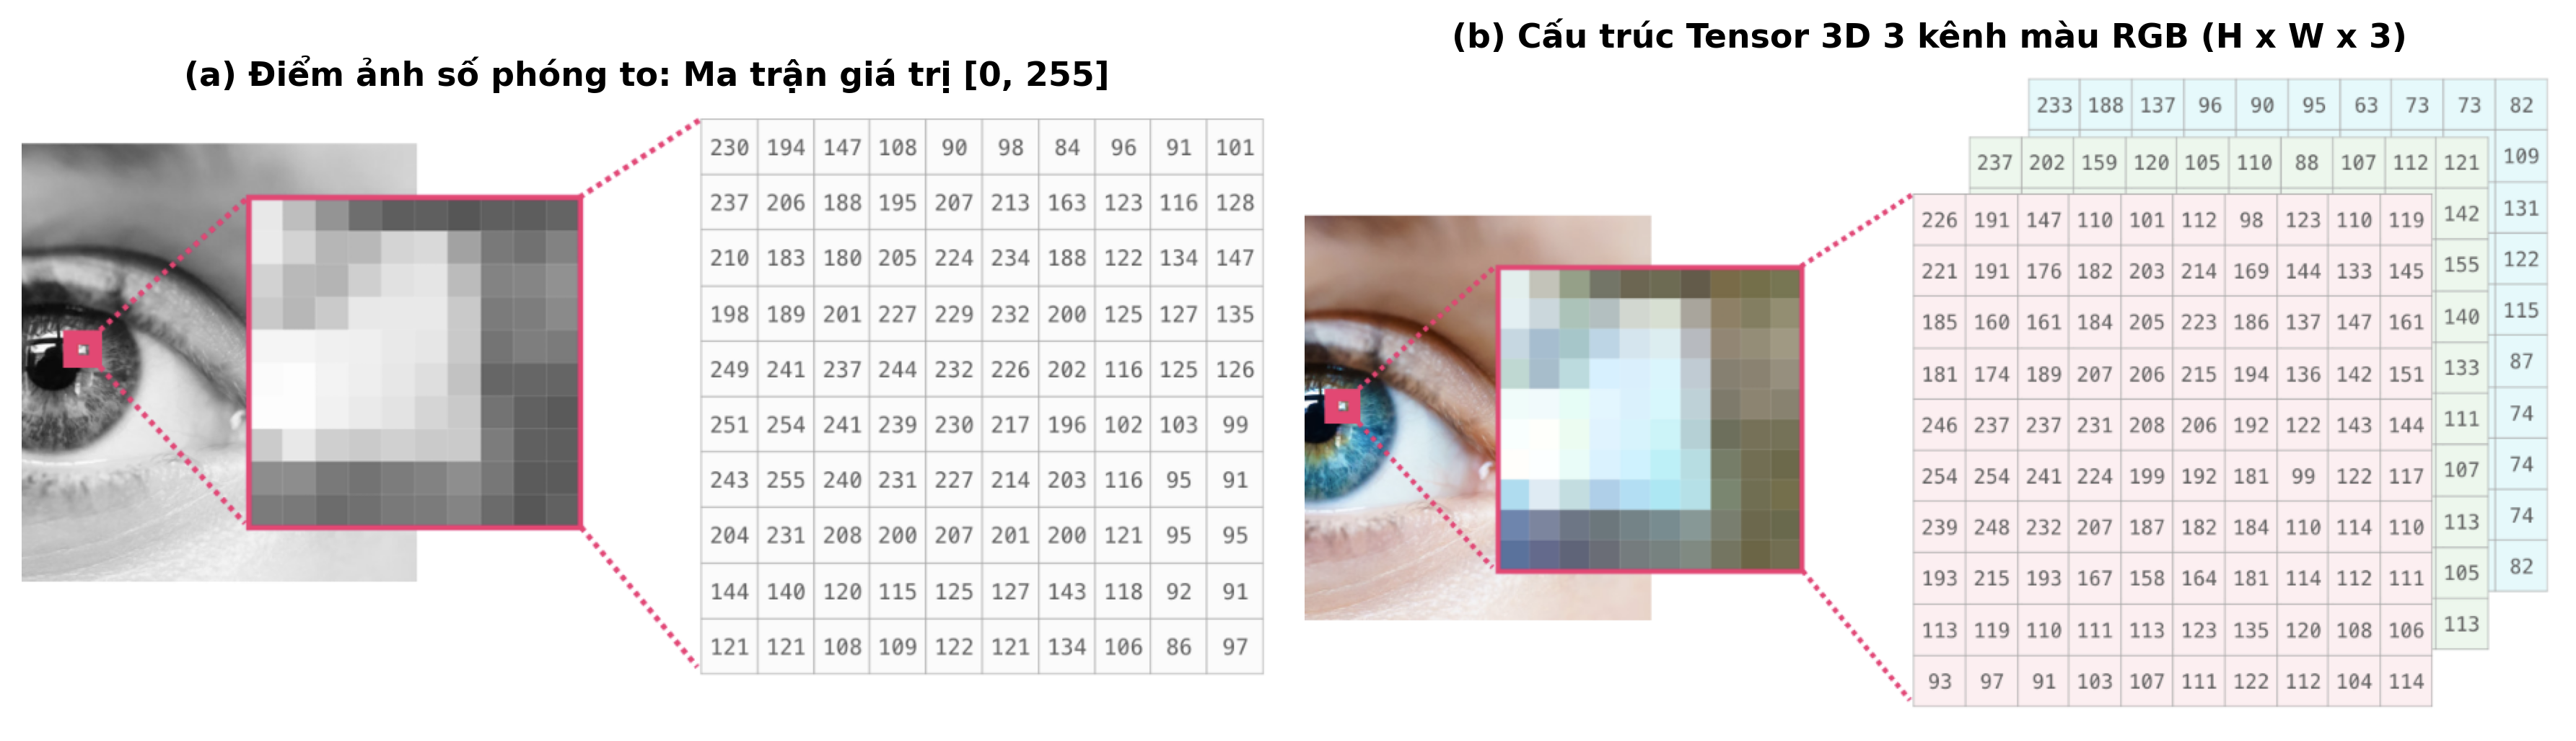
\includegraphics[width=0.92\textwidth]{images/fig00_image_matrix_and_tensor_representation.png}
    \caption{Biểu diễn ảnh số từ Ma trận Pixel rời rạc đến Tensor 3D/4D trong không gian tính toán học sâu.}
    \label{fig:cnn_image_tensor}
\end{figure}

\subsection{Toán Học Phép Toán Tích Chập 2 Chiều (2D Convolution)}
Trong học sâu, phép toán tích chập thực chất là phép toán tương quan chéo (cross-correlation). Cho một tensor đầu vào $\mathbf{X} \in \mathbb{R}^{C_{\text{in}} \times H \times W}$ và một tập hợp gồm $C_{\text{out}}$ bộ lọc (filters/kernels) $\mathbf{K} \in \mathbb{R}^{C_{\text{out}} \times C_{\text{in}} \times k_h \times k_w}$, giá trị tại vị trí $(i, j)$ của bản đồ đặc trưng đầu ra (feature map) thuộc kênh thứ $c$ được xác định bởi:
\begin{equation}
\mathbf{Y}_{c, i, j} = \sum_{m=1}^{C_{\text{in}}} \sum_{u=0}^{k_h - 1} \sum_{v=0}^{k_w - 1} \mathbf{X}_{m, \, i \cdot s + u, \, j \cdot s + v} \cdot \mathbf{K}_{c, m, u, v} + b_c
\end{equation}
trong đó $s$ là bước trượt (stride), và $b_c$ là bias của bộ lọc thứ $c$. Kích thước không gian của bản đồ đặc trưng đầu ra phụ thuộc vào kích thước đầu vào $(H, W)$, kích thước bộ lọc $(k_h, k_w)$, đệm số không (padding $p$) và bước trượt $s$:
\begin{equation}
H_{\text{out}} = \left\lfloor \frac{H - k_h + 2p}{s} \right\rfloor + 1, \qquad W_{\text{out}} = \left\lfloor \frac{W - k_w + 2p}{s} \right\rfloor + 1
\end{equation}

\begin{figure}[H]
    \centering
    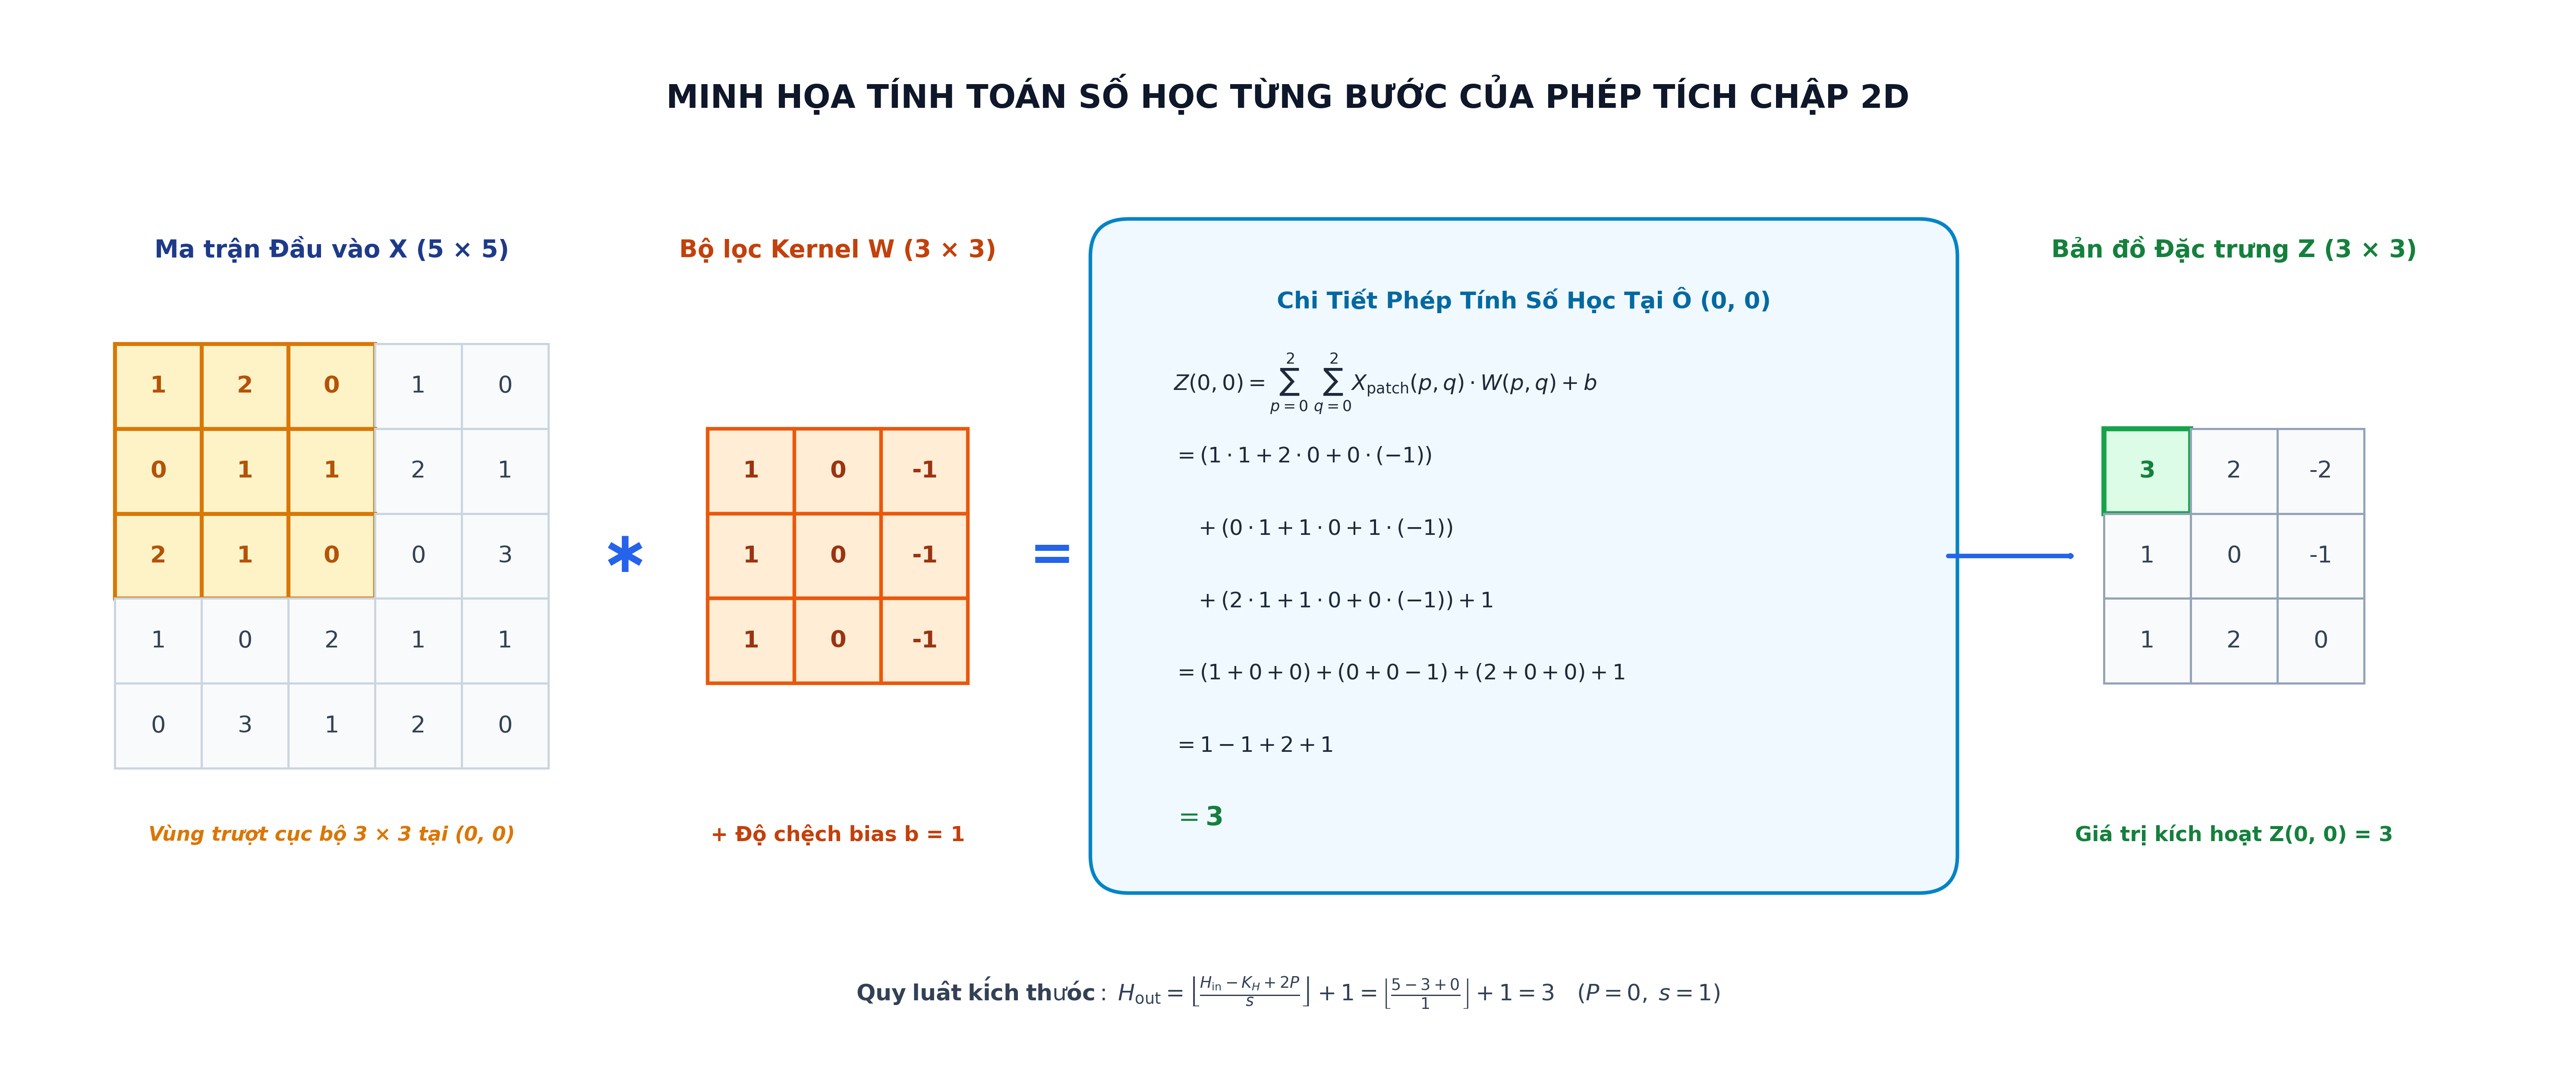
\includegraphics[width=0.95\textwidth]{images/fig06_numerical_convolution_step_by_step.png}
    \caption{Minh họa số học chi tiết từng bước trượt của phép toán tích chập 2D trên ma trận điểm ảnh.}
    \label{fig:cnn_conv_numeric}
\end{figure}

\subsection{Vùng Cảm Nhận (Receptive Field) và Phép Gộp (Pooling)}
Vùng cảm nhận (Receptive Field -- RF) là kích thước vùng không gian trên ảnh đầu vào mà một nơ-ron ở tầng sâu có thể “quan sát” được. Khi xếp chồng liên tiếp các tầng tích chập nhỏ $k \times k$ với bước trượt $s=1$, vùng cảm nhận hiệu dụng $RF_l$ tại tầng $l$ tăng tuyến tính:
\begin{equation}
RF_l = RF_{l-1} + (k_l - 1) \cdot \prod_{i=1}^{l-1} s_i
\end{equation}
Nguyên lý này là nền tảng của kiến trúc VGG: thay vì dùng một bộ lọc lớn $5 \times 5$ (đòi hỏi $25$ trọng số), việc xếp chồng 2 tầng $3 \times 3$ liên tiếp cho cùng một vùng cảm nhận $5 \times 5$ nhưng chỉ tiêu tốn $2 \times (3 \times 3) = 18$ trọng số (giảm $28\%$ tham số) và tăng gấp đôi số hàm phi tuyến ReLU.

\begin{figure}[H]
    \centering
    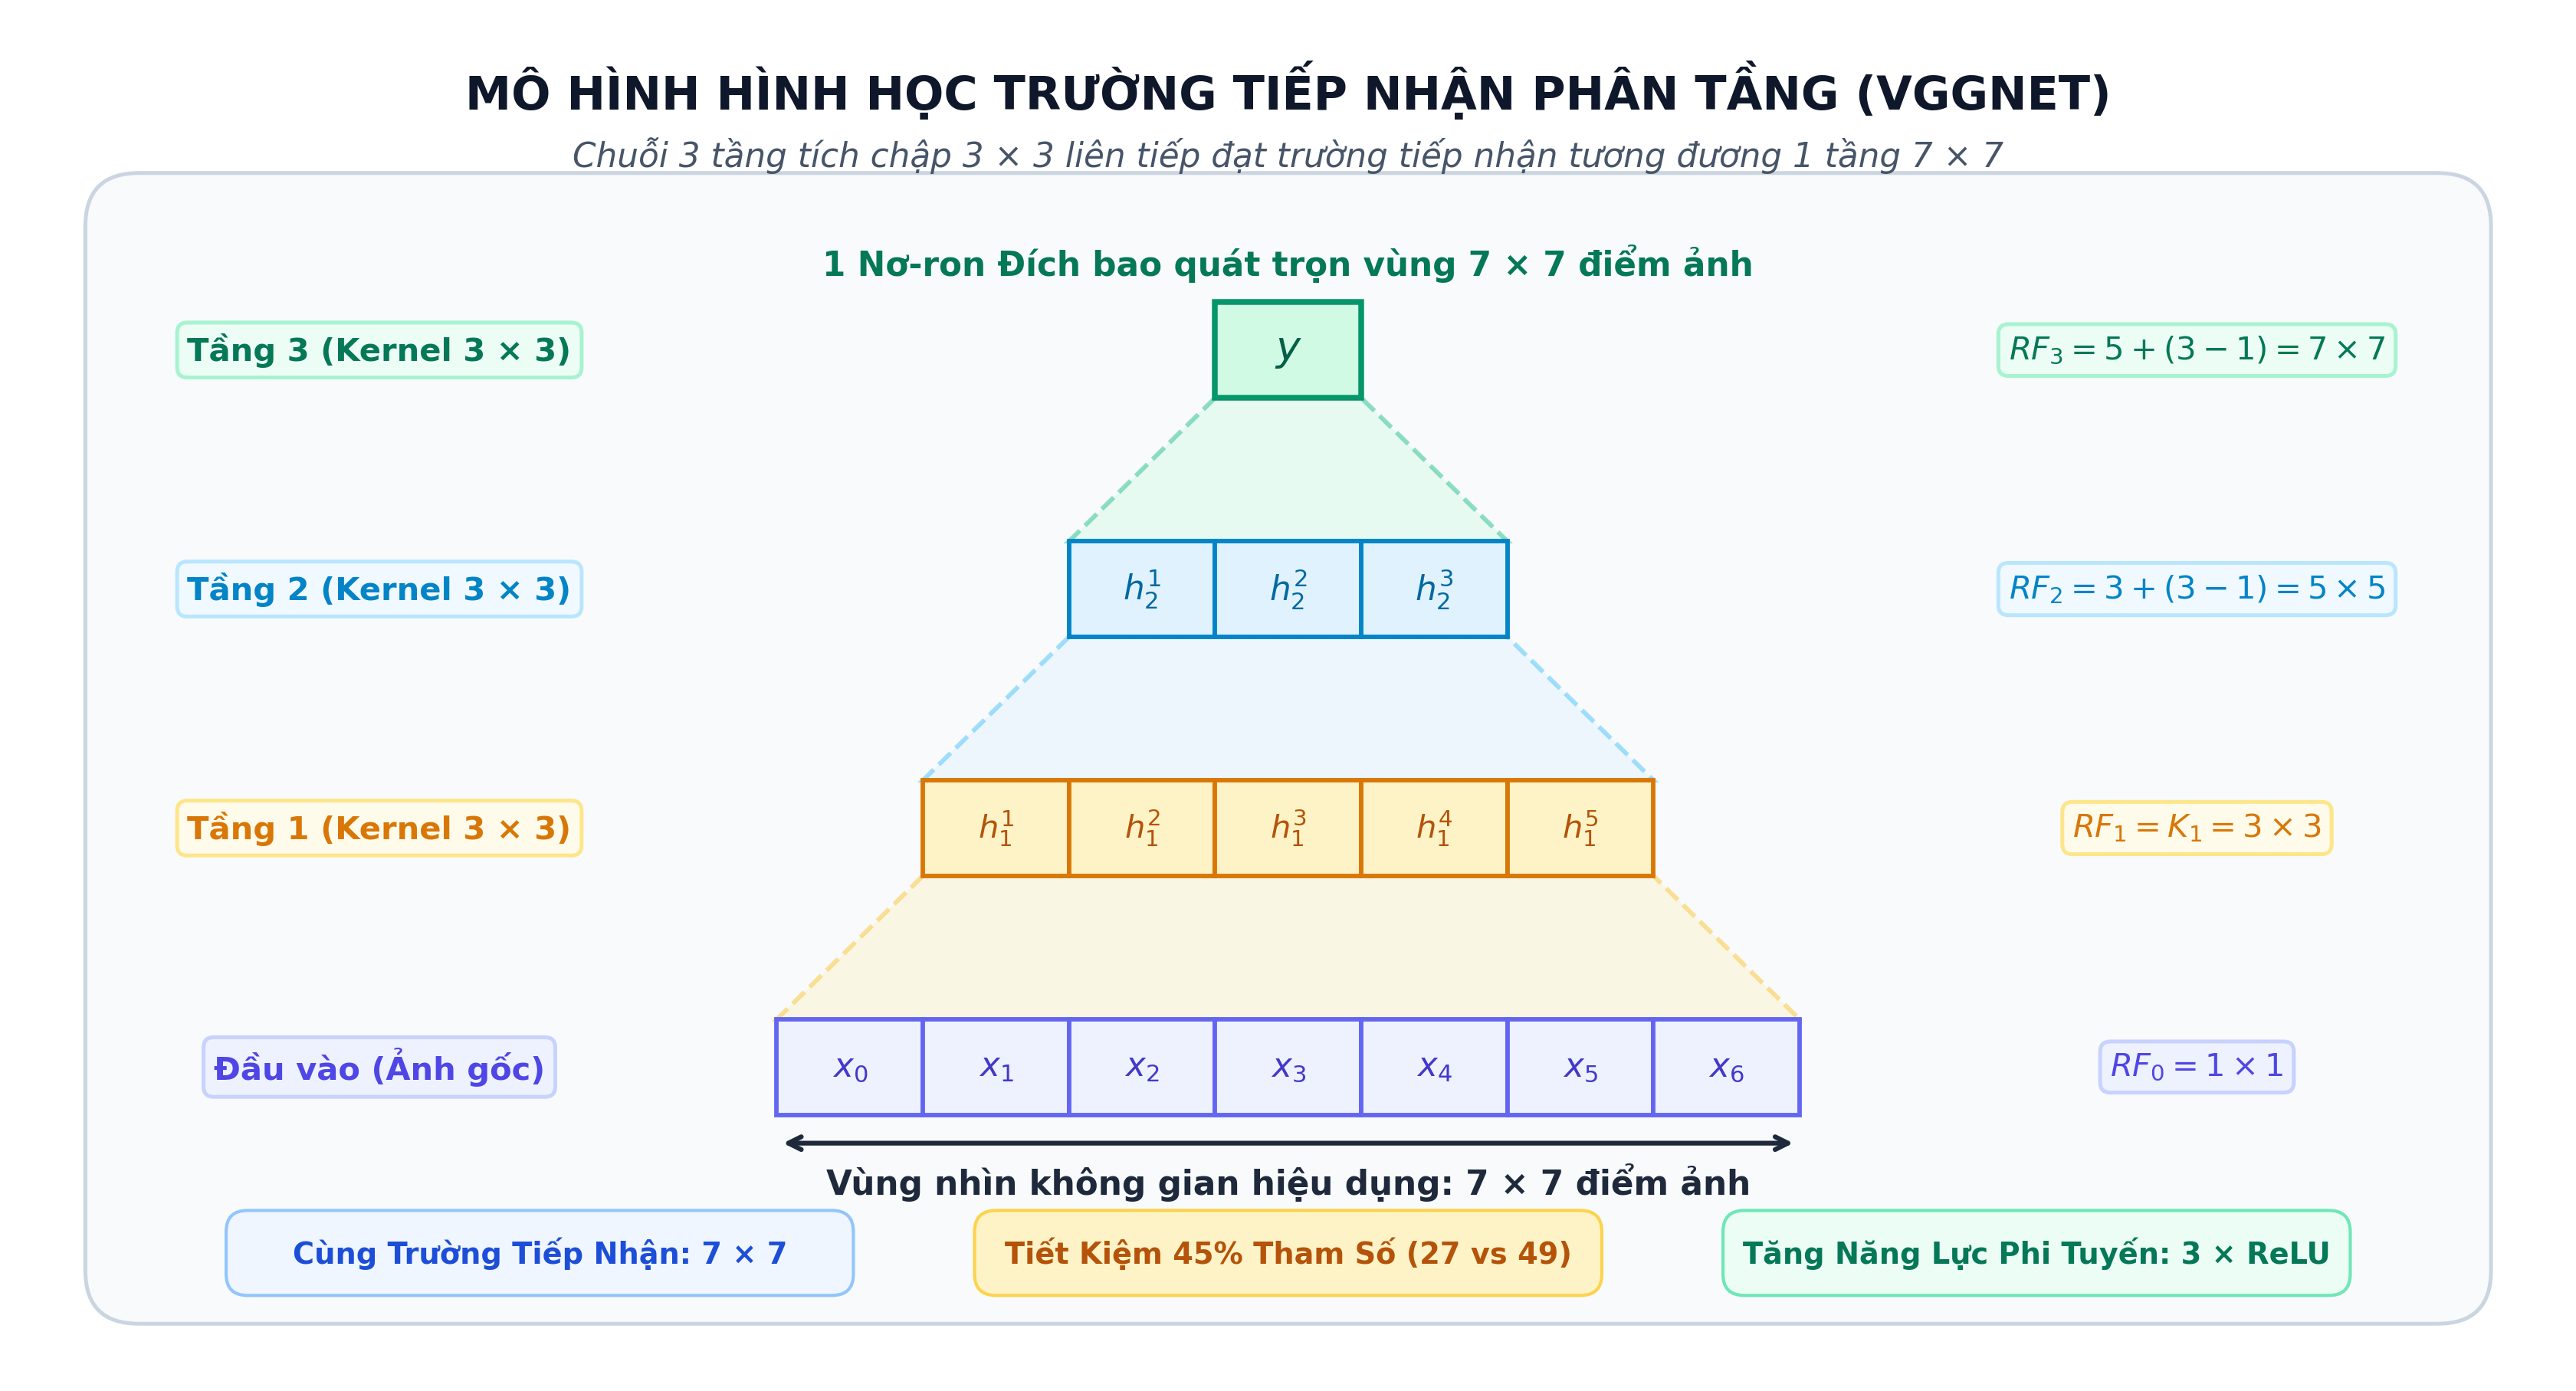
\includegraphics[width=0.92\textwidth]{images/fig07_receptive_field_stacking.png}
    \caption{Cơ chế tích lũy vùng cảm nhận (Receptive Field) khi xếp chồng các bộ lọc tích chập nhỏ.}
    \label{fig:cnn_rf}
\end{figure}

\begin{figure}[H]
    \centering
    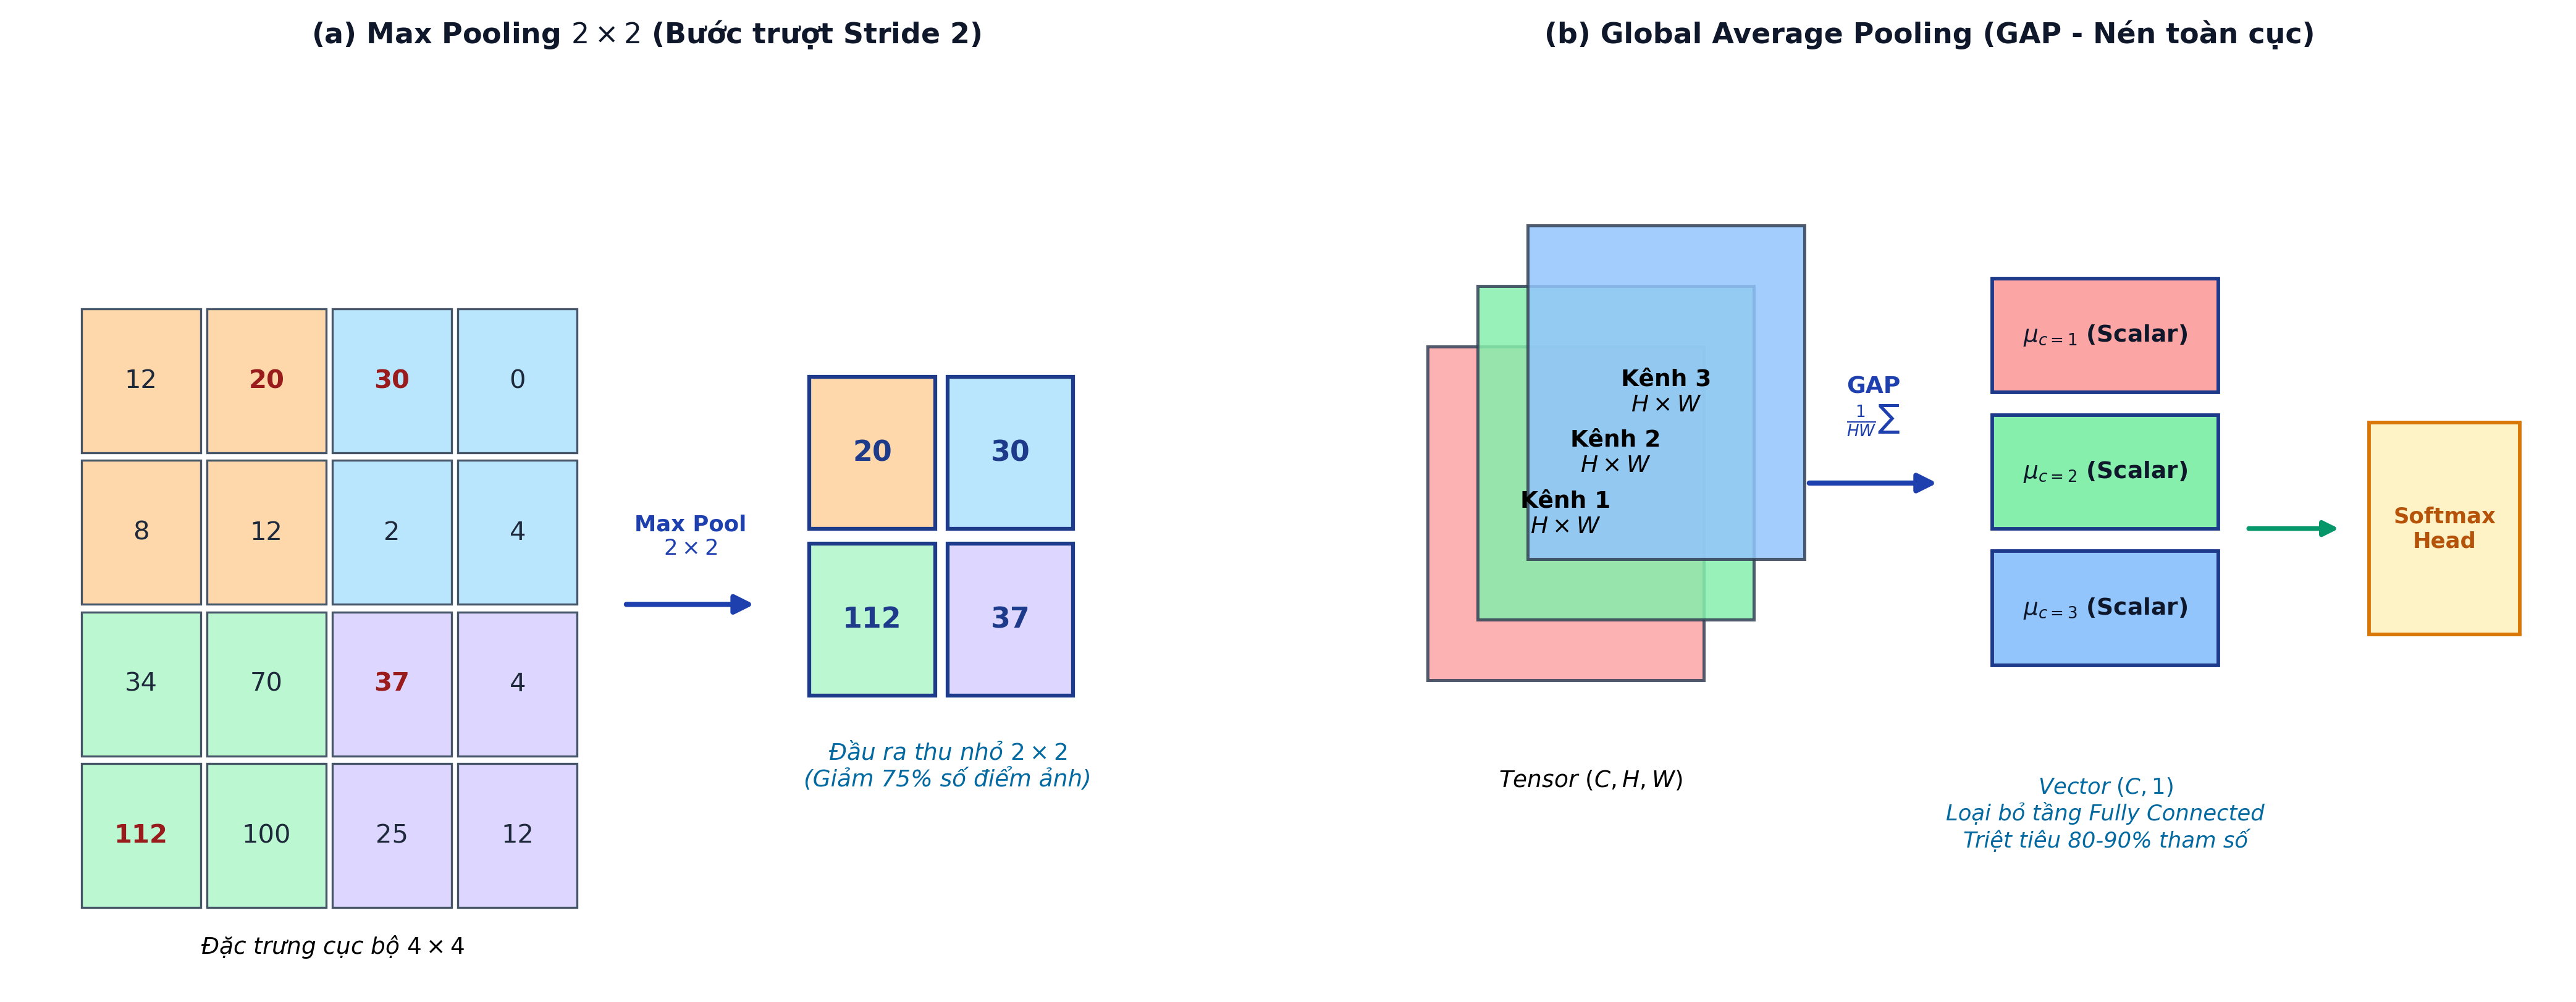
\includegraphics[width=0.92\textwidth]{images/fig03_pooling_and_gap_comparison.png}
    \caption{So sánh cơ chế hoạt động của Max Pooling, Average Pooling và Global Average Pooling (GAP).}
    \label{fig:cnn_pooling}
\end{figure}

Phép gộp (Spatial Pooling) thực hiện lấy mẫu giảm kích thước không gian nhằm tăng tính bất biến trước các biến đổi co dãn, dịch chuyển nhỏ, đồng thời mở rộng nhanh vùng cảm nhận cho các tầng tiếp theo:
\begin{itemize}[leftmargin=1.2cm]
    \item \textbf{Max Pooling:} Chọn giá trị cực đại trong vùng cửa sổ, giữ lại các đặc trưng biên và vân bề mặt có cường độ kích hoạt mạnh nhất.
    \item \textbf{Global Average Pooling (GAP) (Lin et al., 2013):} Tính trung bình cộng toàn bộ không gian của mỗi bản đồ đặc trưng, biến tensor $\mathbb{R}^{C \times H \times W}$ trực tiếp thành vector $\mathbb{R}^C$. GAP loại bỏ hoàn toàn các tầng kết nối đầy đủ (Dense layers) cồng kềnh, giảm hàng chục triệu tham số và chống quá khớp triệt để.
\end{itemize}

\subsection{Tiến Hóa Kiến Trúc: VGG, ResNet và MobileNet}

\begin{figure}[H]
    \centering
    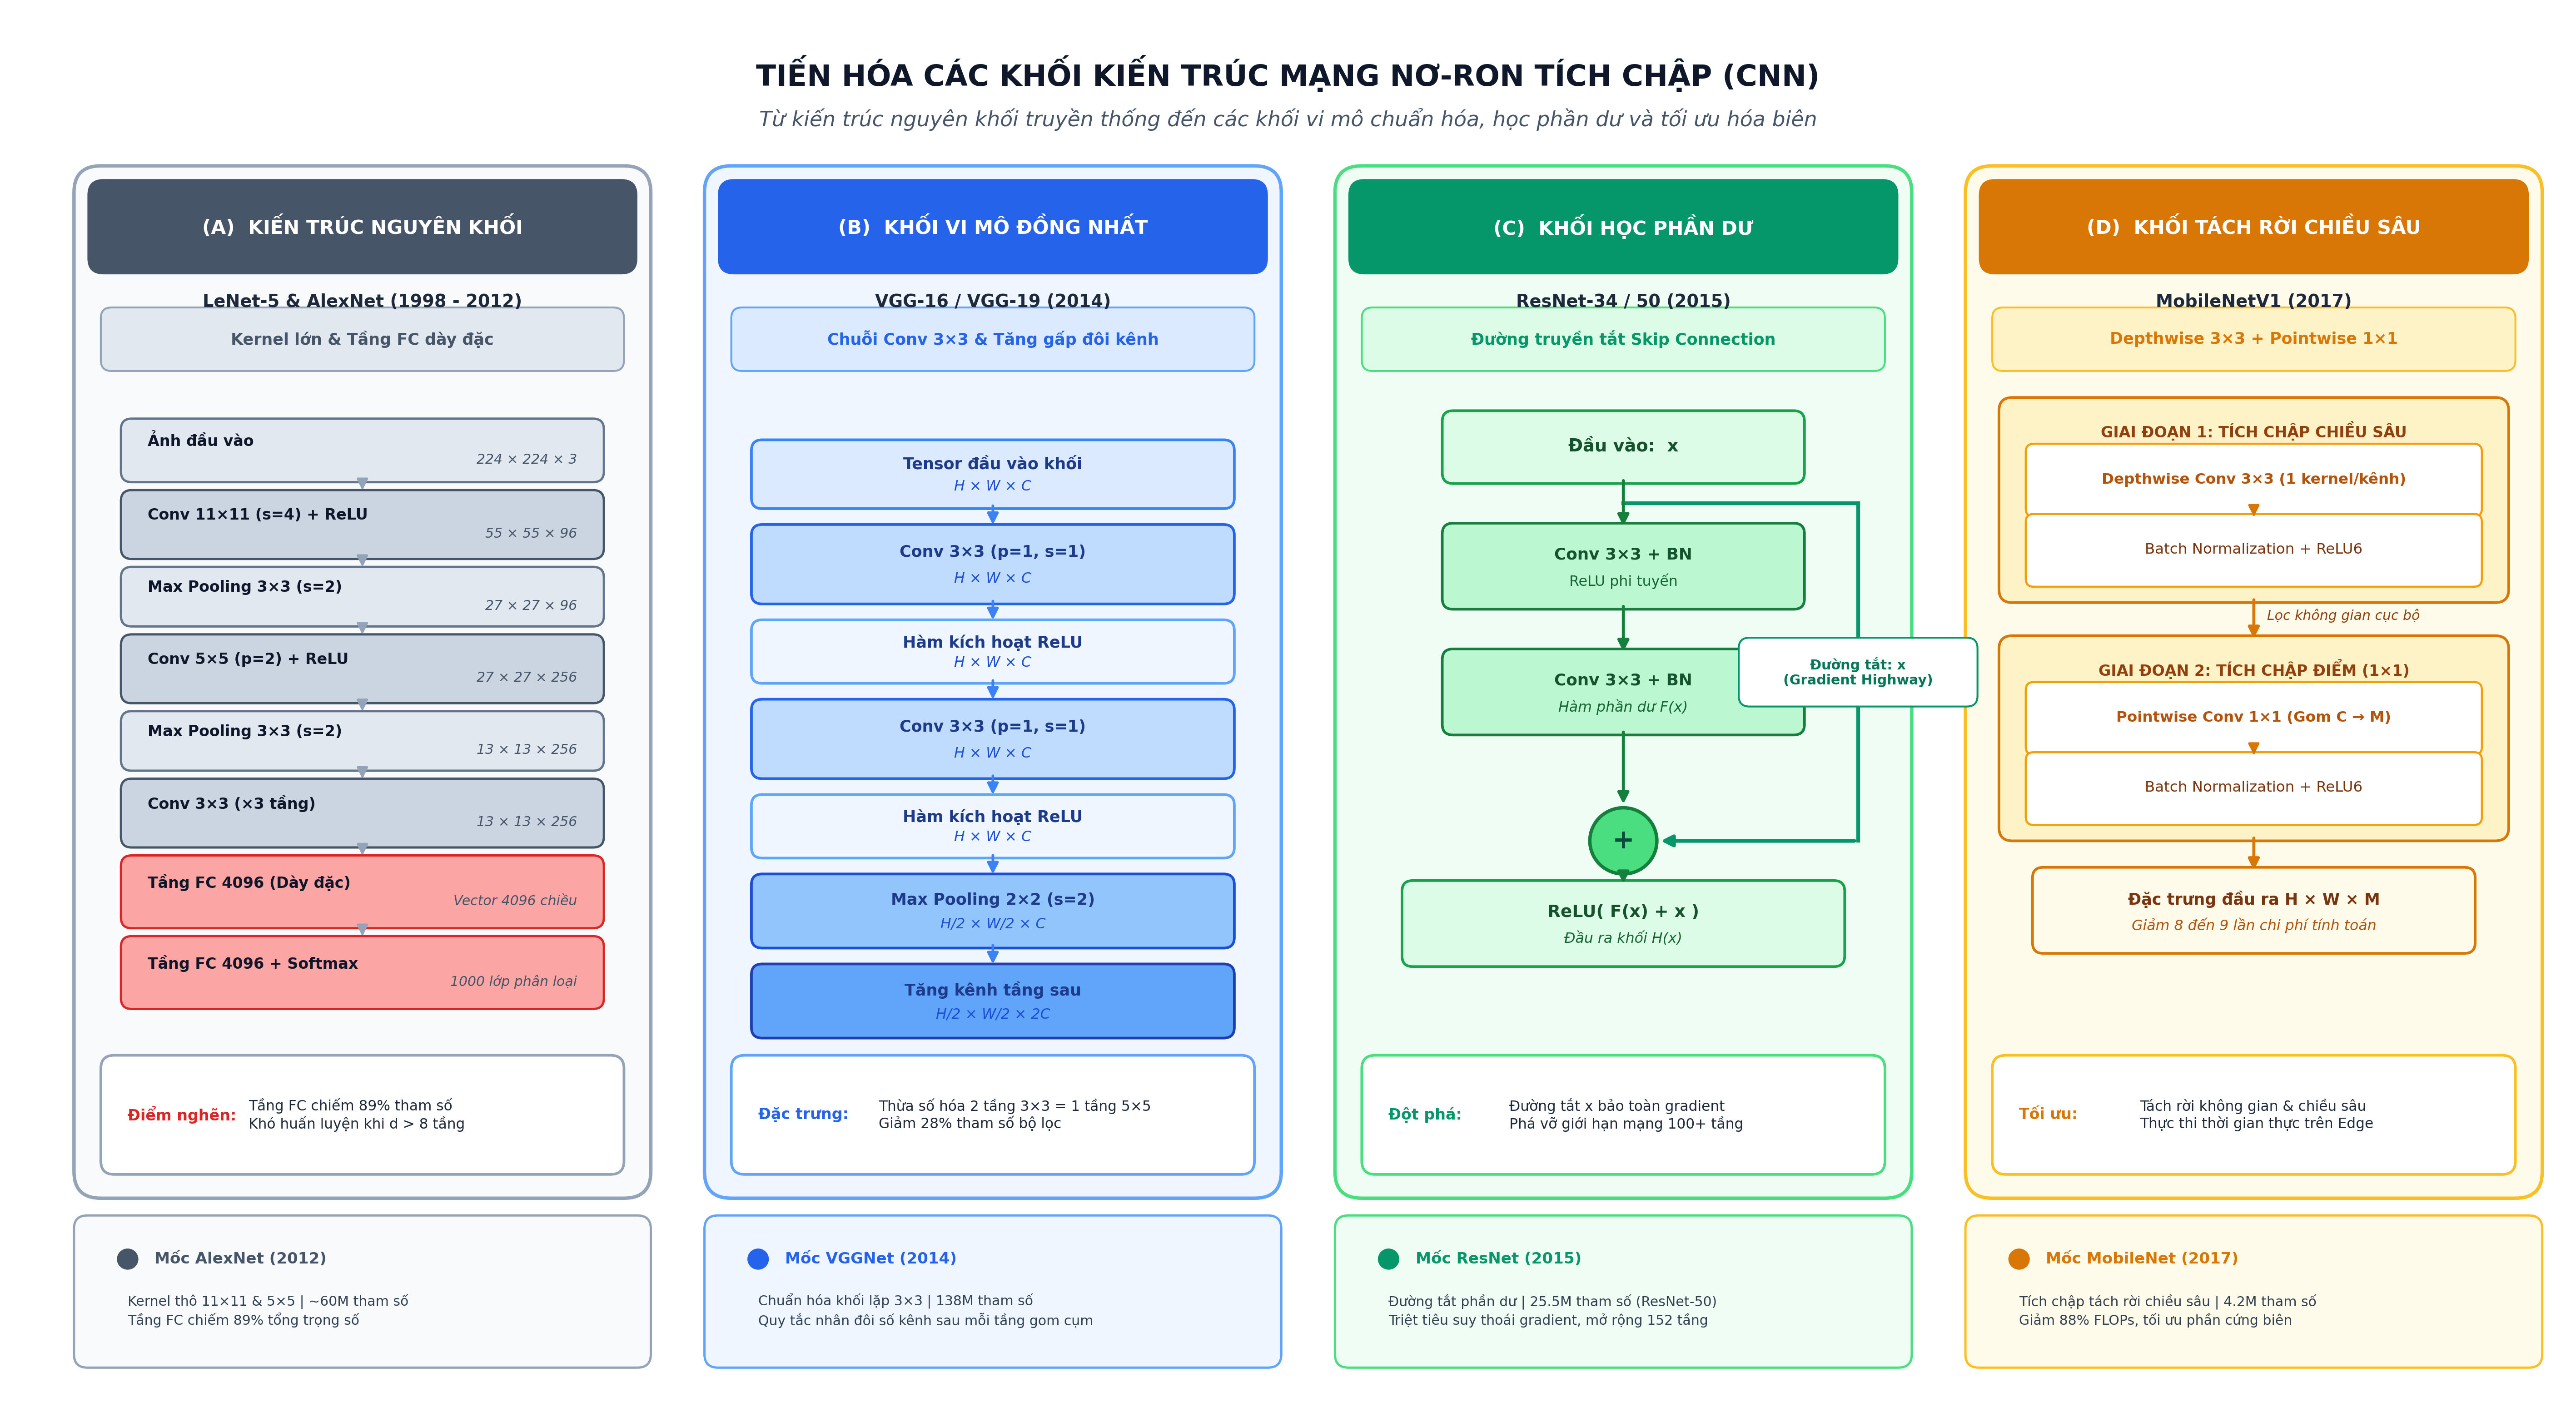
\includegraphics[width=\textwidth]{images/fig201_cnn_evolution_blocks.png}
    \caption{Sơ đồ tiến hóa kiến trúc CNN: Từ khối tích chập phẳng đến khối Residual (ResNet) và Tích chập tách biệt chiều sâu (MobileNet).}
    \label{fig:cnn_blocks_evolution}
\end{figure}

\begin{figure}[H]
    \centering
    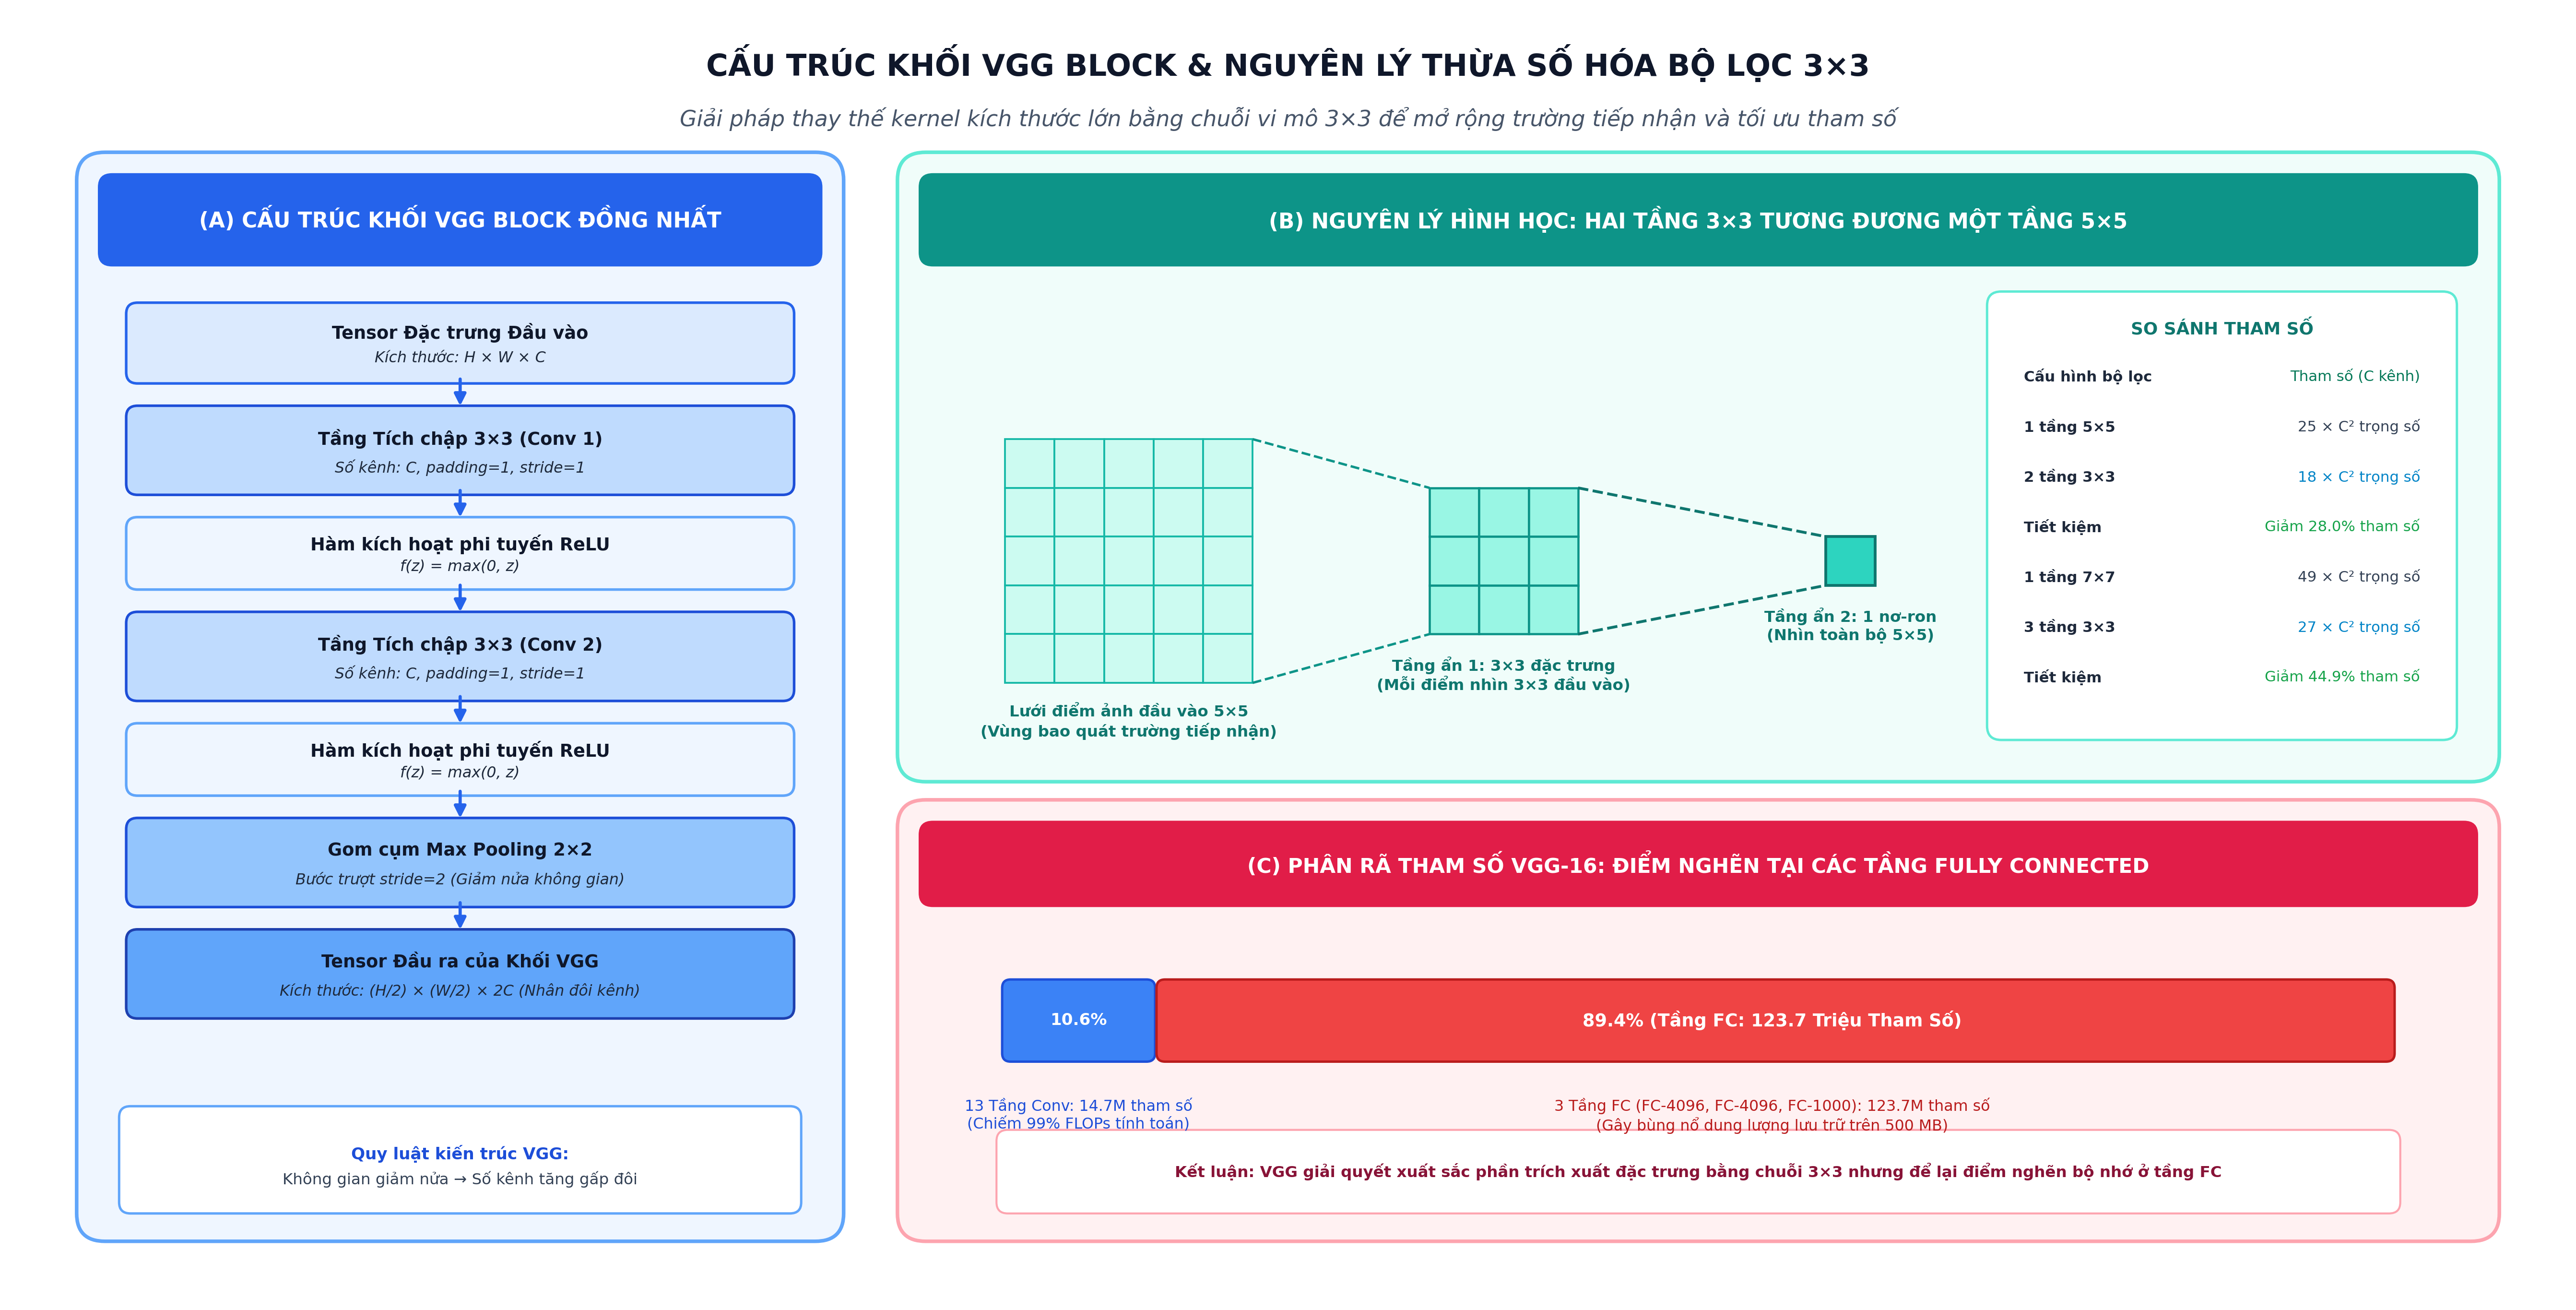
\includegraphics[width=0.90\textwidth]{images/fig202_vgg_block_and_receptive_field.png}
    \caption{Kiến trúc khối VGG Block và cơ chế tương đương vùng cảm nhận của các bộ lọc $3 \times 3$.}
    \label{fig:cnn_vgg_block}
\end{figure}

\begin{figure}[H]
    \centering
    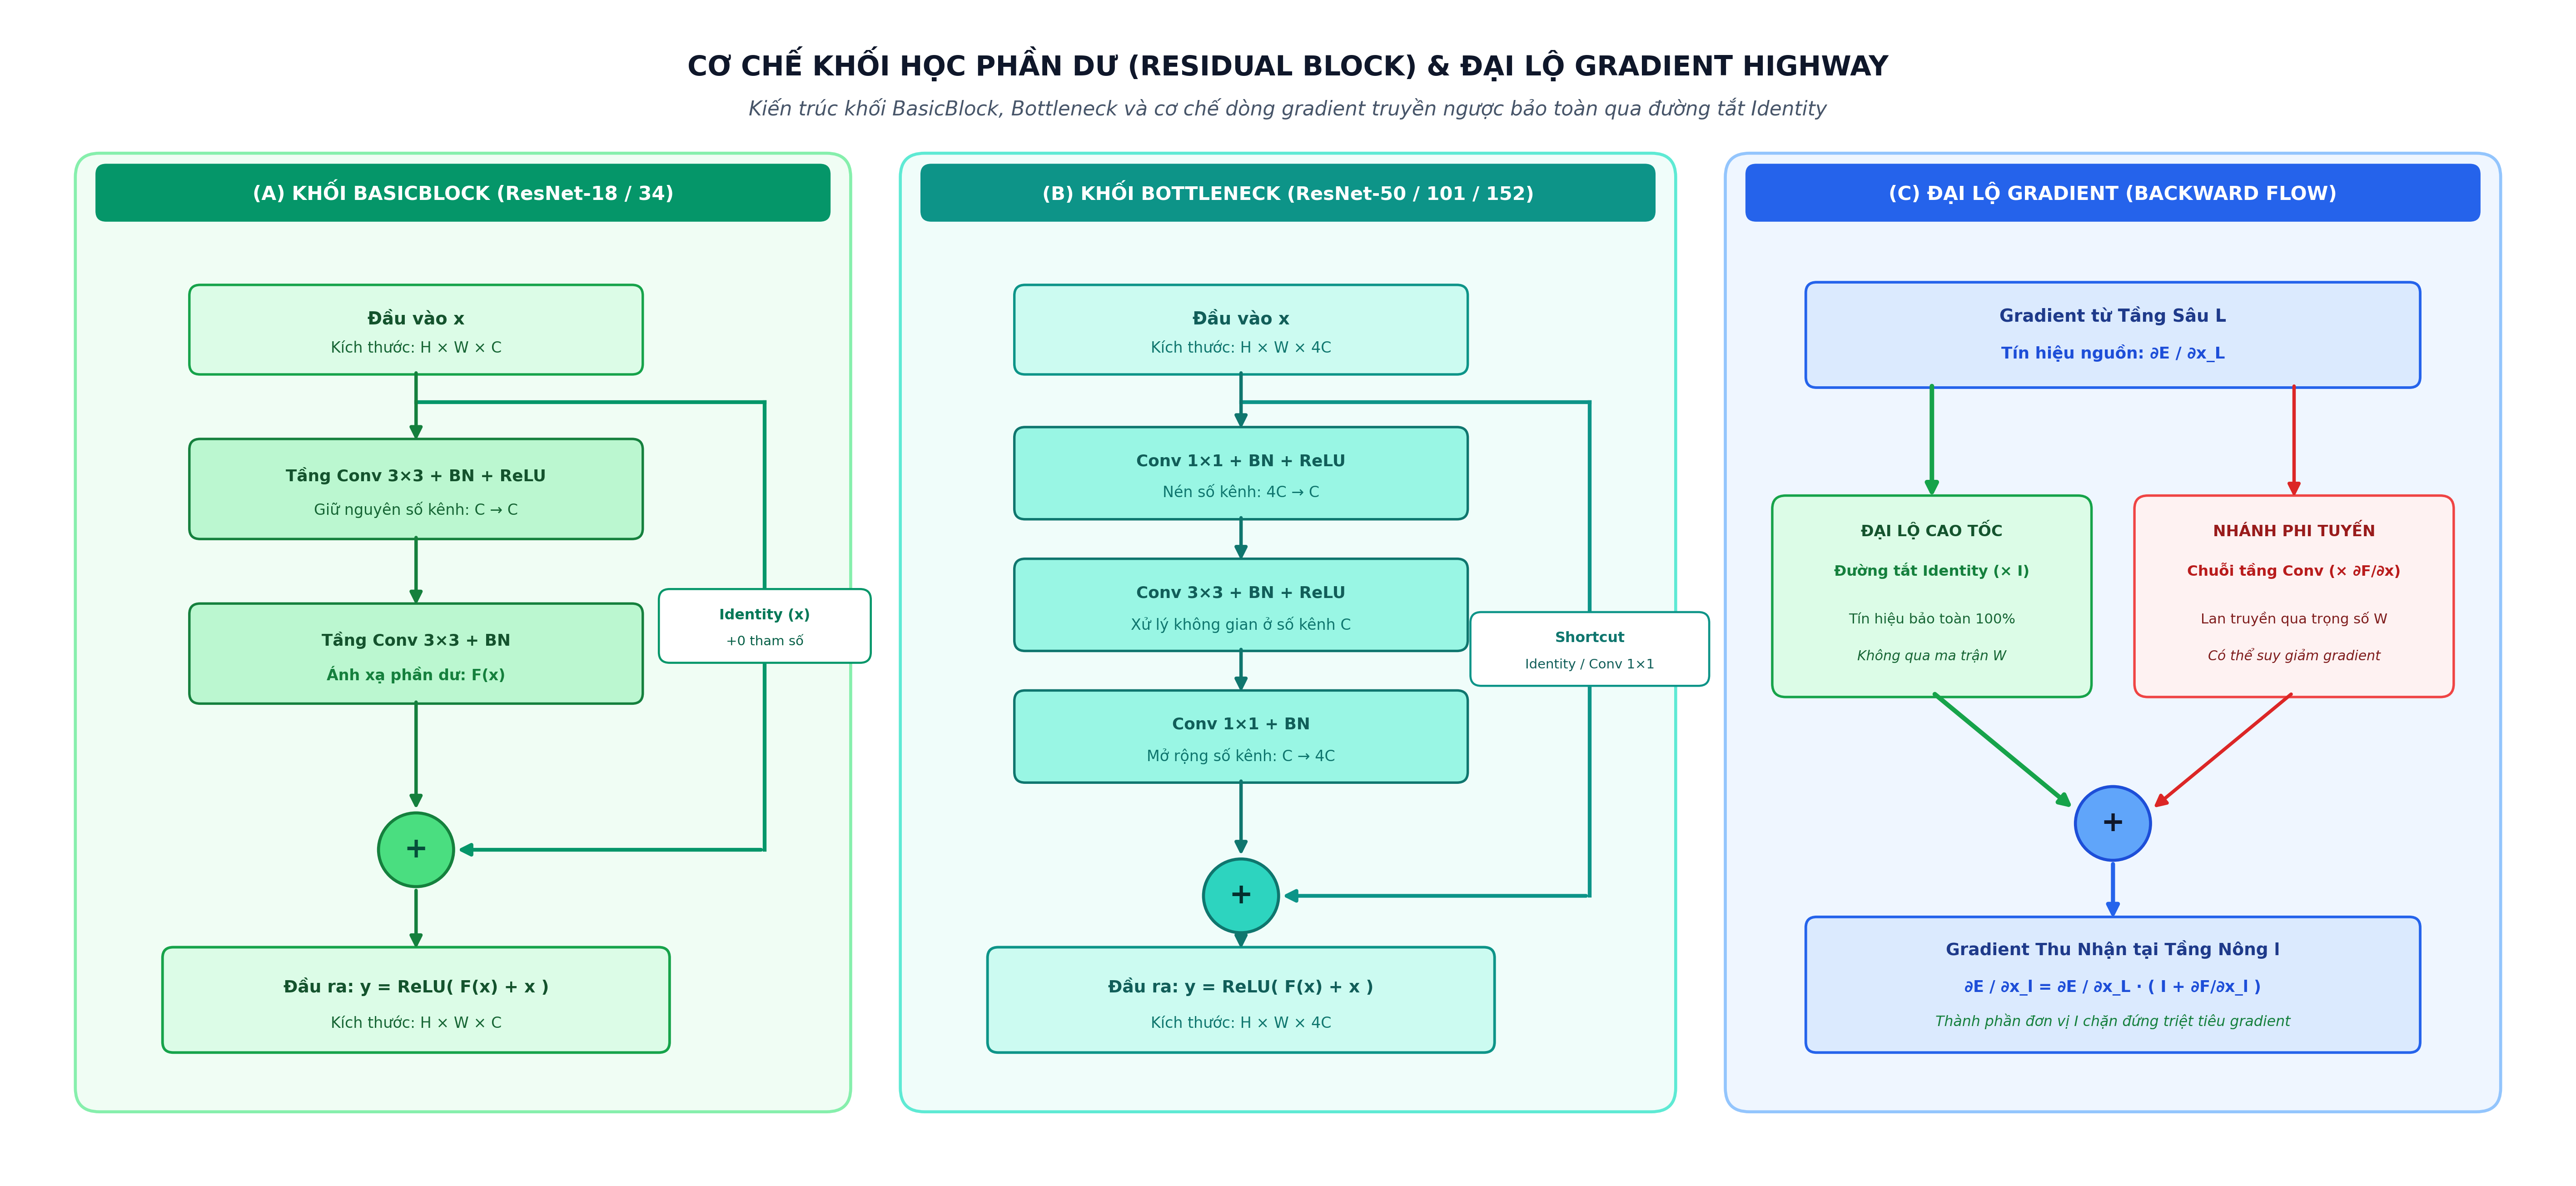
\includegraphics[width=0.90\textwidth]{images/fig203_resnet_residual_block_and_gradient.png}
    \caption{Kiến trúc khối phần dư Residual Block (ResNet) và cơ chế “đường cao tốc” dòng gradient.}
    \label{fig:cnn_resnet_block}
\end{figure}

\begin{figure}[H]
    \centering
    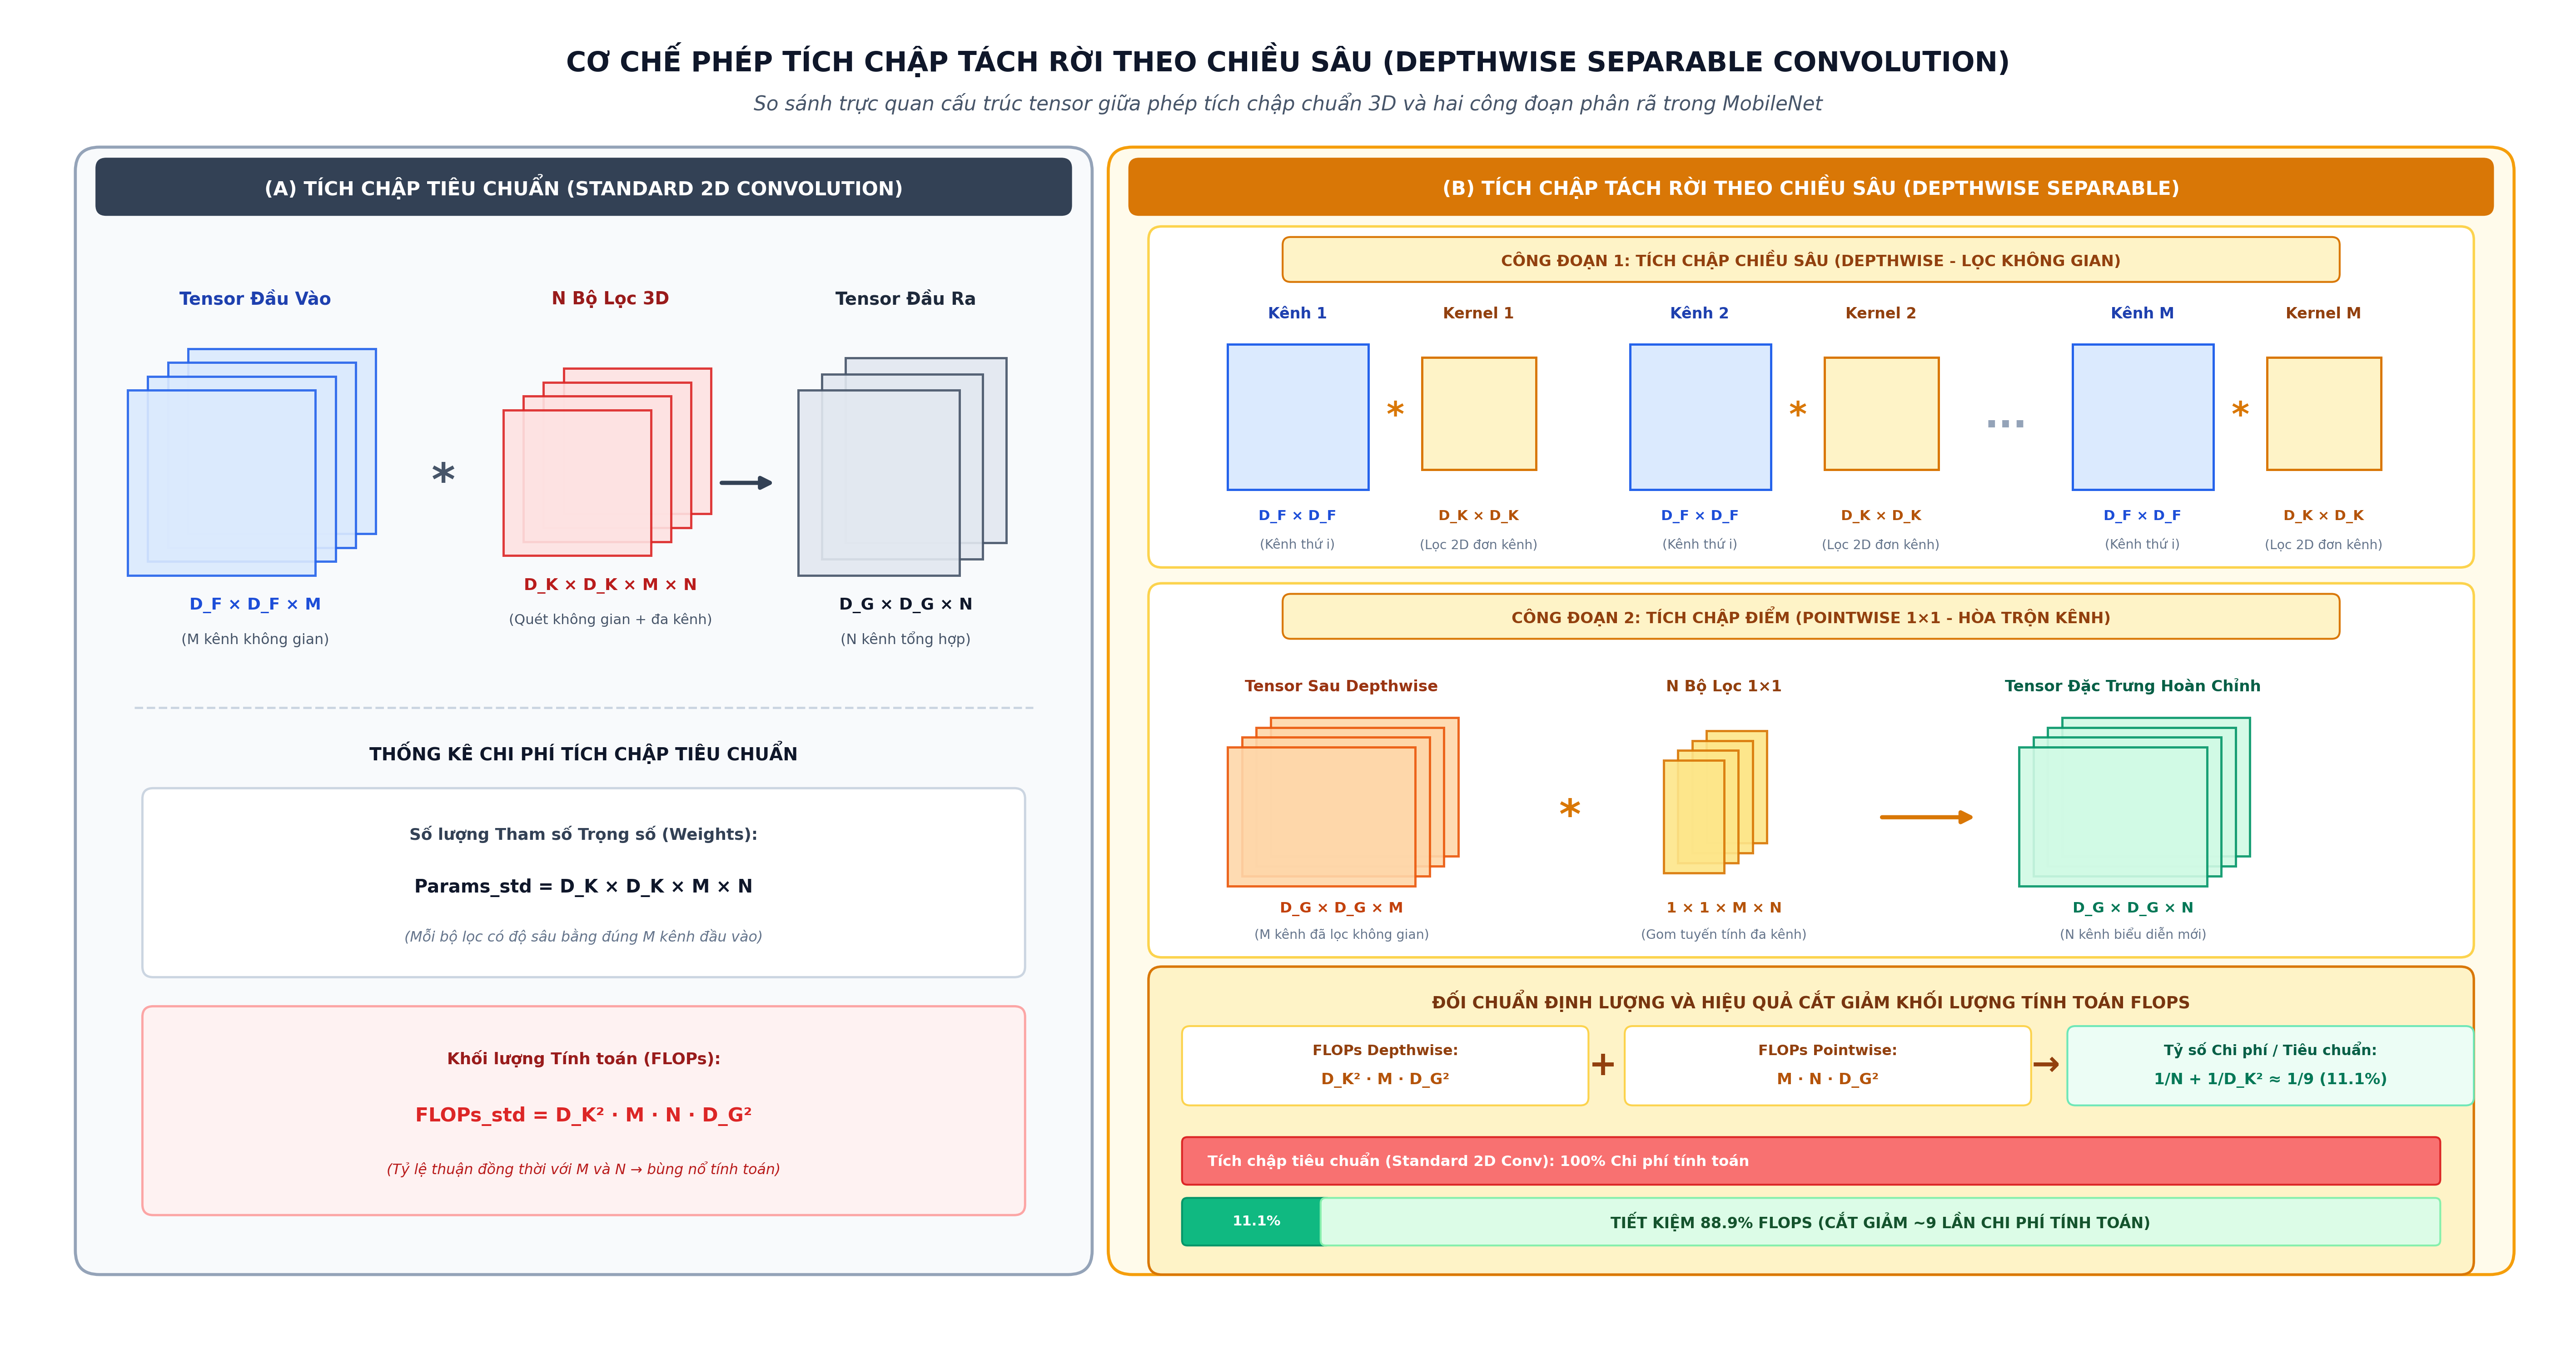
\includegraphics[width=0.90\textwidth]{images/fig204_mobilenet_depthwise_separable.png}
    \caption{Kiến trúc Depthwise Separable Convolution trong MobileNet: Tách biệt hoàn toàn không gian và kênh màu.}
    \label{fig:cnn_mobilenet_block}
\end{figure}

\begin{itemize}[leftmargin=1.2cm]
    \item \textbf{Khối Residual (ResNet - He et al., 2015):} Giải quyết hiện tượng thoái hóa mạng sâu bằng kết nối tắt: $\mathbf{y} = \mathcal{F}(\mathbf{x}) + \mathbf{x}$. Đạo hàm theo quy tắc dây chuyền:
    \begin{equation}
    \frac{\partial \mathcal{E}}{\partial \mathbf{x}} = \frac{\partial \mathcal{E}}{\partial \mathbf{y}} \left( \frac{\partial \mathcal{F}}{\partial \mathbf{x}} + \mathbf{I} \right)
    \end{equation}
    Thành phần ma trận đơn vị $\mathbf{I}$ đảm bảo gradient luôn có một “đường cao tốc” truyền thẳng về các tầng đầu tiên mà không bao giờ bị triệt tiêu về 0, ngay cả khi các trọng số của $\mathcal{F}$ tiến về 0.
    \item \textbf{Depthwise Separable Convolution (MobileNet - Howard et al., 2017):} Phân rã phép tích chập chuẩn:
    \begin{enumerate}
        \item \textit{Depthwise Conv:} Áp dụng 1 bộ lọc $k \times k$ cho mỗi kênh đầu vào độc lập: Chi phí $C_{\text{in}} \cdot H \cdot W \cdot k^2$.
        \item \textit{Pointwise Conv:} Áp dụng $C_{\text{out}}$ bộ lọc $1 \times 1 \times C_{\text{in}}$ để kết hợp tuyến tính các kênh: Chi phí $C_{\text{in}} \cdot C_{\text{out}} \cdot H \cdot W$.
    \end{enumerate}
    Tỷ lệ chi phí tính toán so với tích chập tiêu chuẩn là:
    \begin{equation}
    \frac{\text{Chi phí MobileNet}}{\text{Chi phí Standard Conv}} = \frac{C_{\text{in}} \cdot H \cdot W \cdot k^2 + C_{\text{in}} \cdot C_{\text{out}} \cdot H \cdot W}{C_{\text{in}} \cdot C_{\text{out}} \cdot H \cdot W \cdot k^2} = \frac{1}{C_{\text{out}}} + \frac{1}{k^2}
    \end{equation}
    Với bộ lọc $3 \times 3$ ($k=3$), chi phí tính toán FLOPs giảm khoảng $\frac{1}{9} \approx 88.9\%$, cho phép các mô hình thị giác chạy thời gian thực trên vi xử lý điện thoại thông minh.
\end{itemize}

\section{Khảo Sát Thực Nghiệm và Tiền Xử Lý 3 Bộ Dữ Liệu Đa Miền}

\subsection{Tập Dữ Liệu 1: Nhận Dạng Chữ Số Nhà SVHN (Street View House Numbers)}
\begin{itemize}[leftmargin=1.2cm]
    \item \textbf{Nguồn gốc dữ liệu:} Tập dữ liệu ảnh số Stanford SVHN thu thập từ ảnh chụp đời thực Google Street View (\url{http://ufldl.stanford.edu/housenumbers/}).
    \item \textbf{Quy mô và kích thước:} Gồm $73,257$ ảnh huấn luyện và $26,032$ ảnh kiểm thử (tổng cộng $99,289$ ảnh), kích thước chuẩn $32 \times 32 \times 3$ điểm ảnh màu RGB, thuộc 10 lớp chữ số từ $0$ đến $9$.
\end{itemize}

\begin{figure}[H]
    \centering
    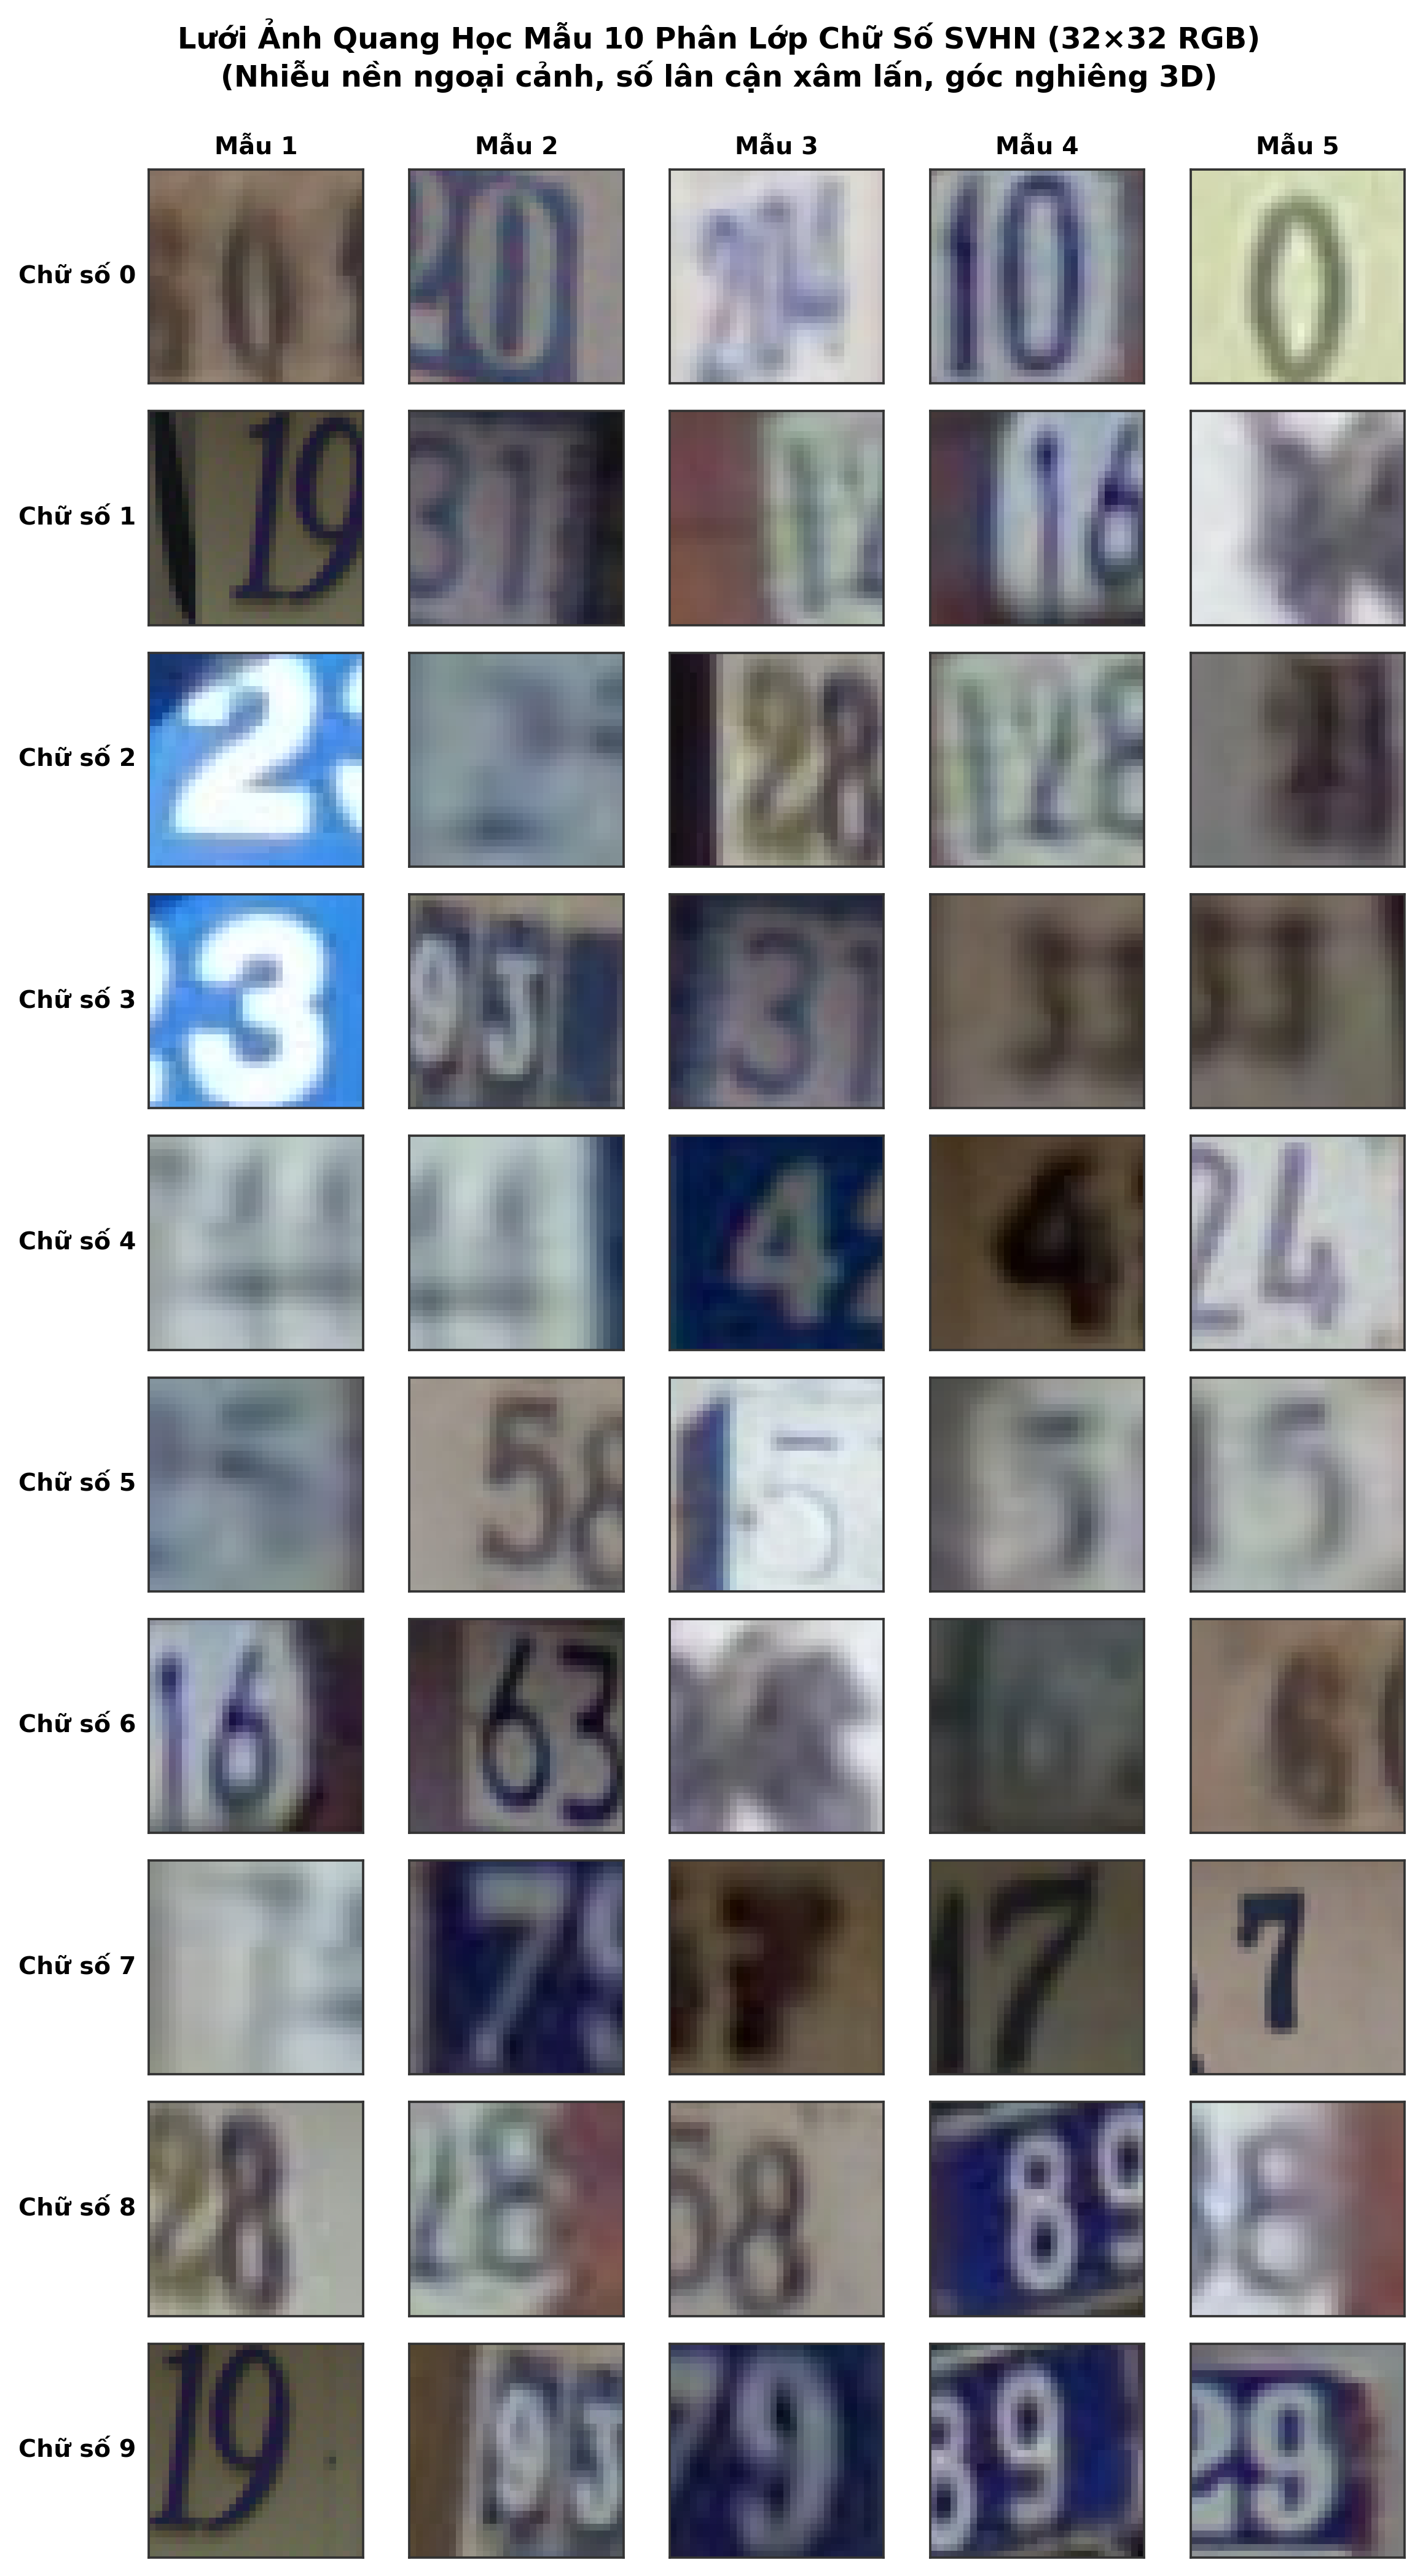
\includegraphics[width=0.90\textwidth]{images/fig404_svhn_sample_grid.png}
    \caption{Lưới mẫu ảnh thực tế từ tập dữ liệu SVHN thể hiện tính đa dạng về ánh sáng, phông nền và biến dạng.}
    \label{fig:svhn_grid}
\end{figure}

\begin{figure}[H]
    \centering
    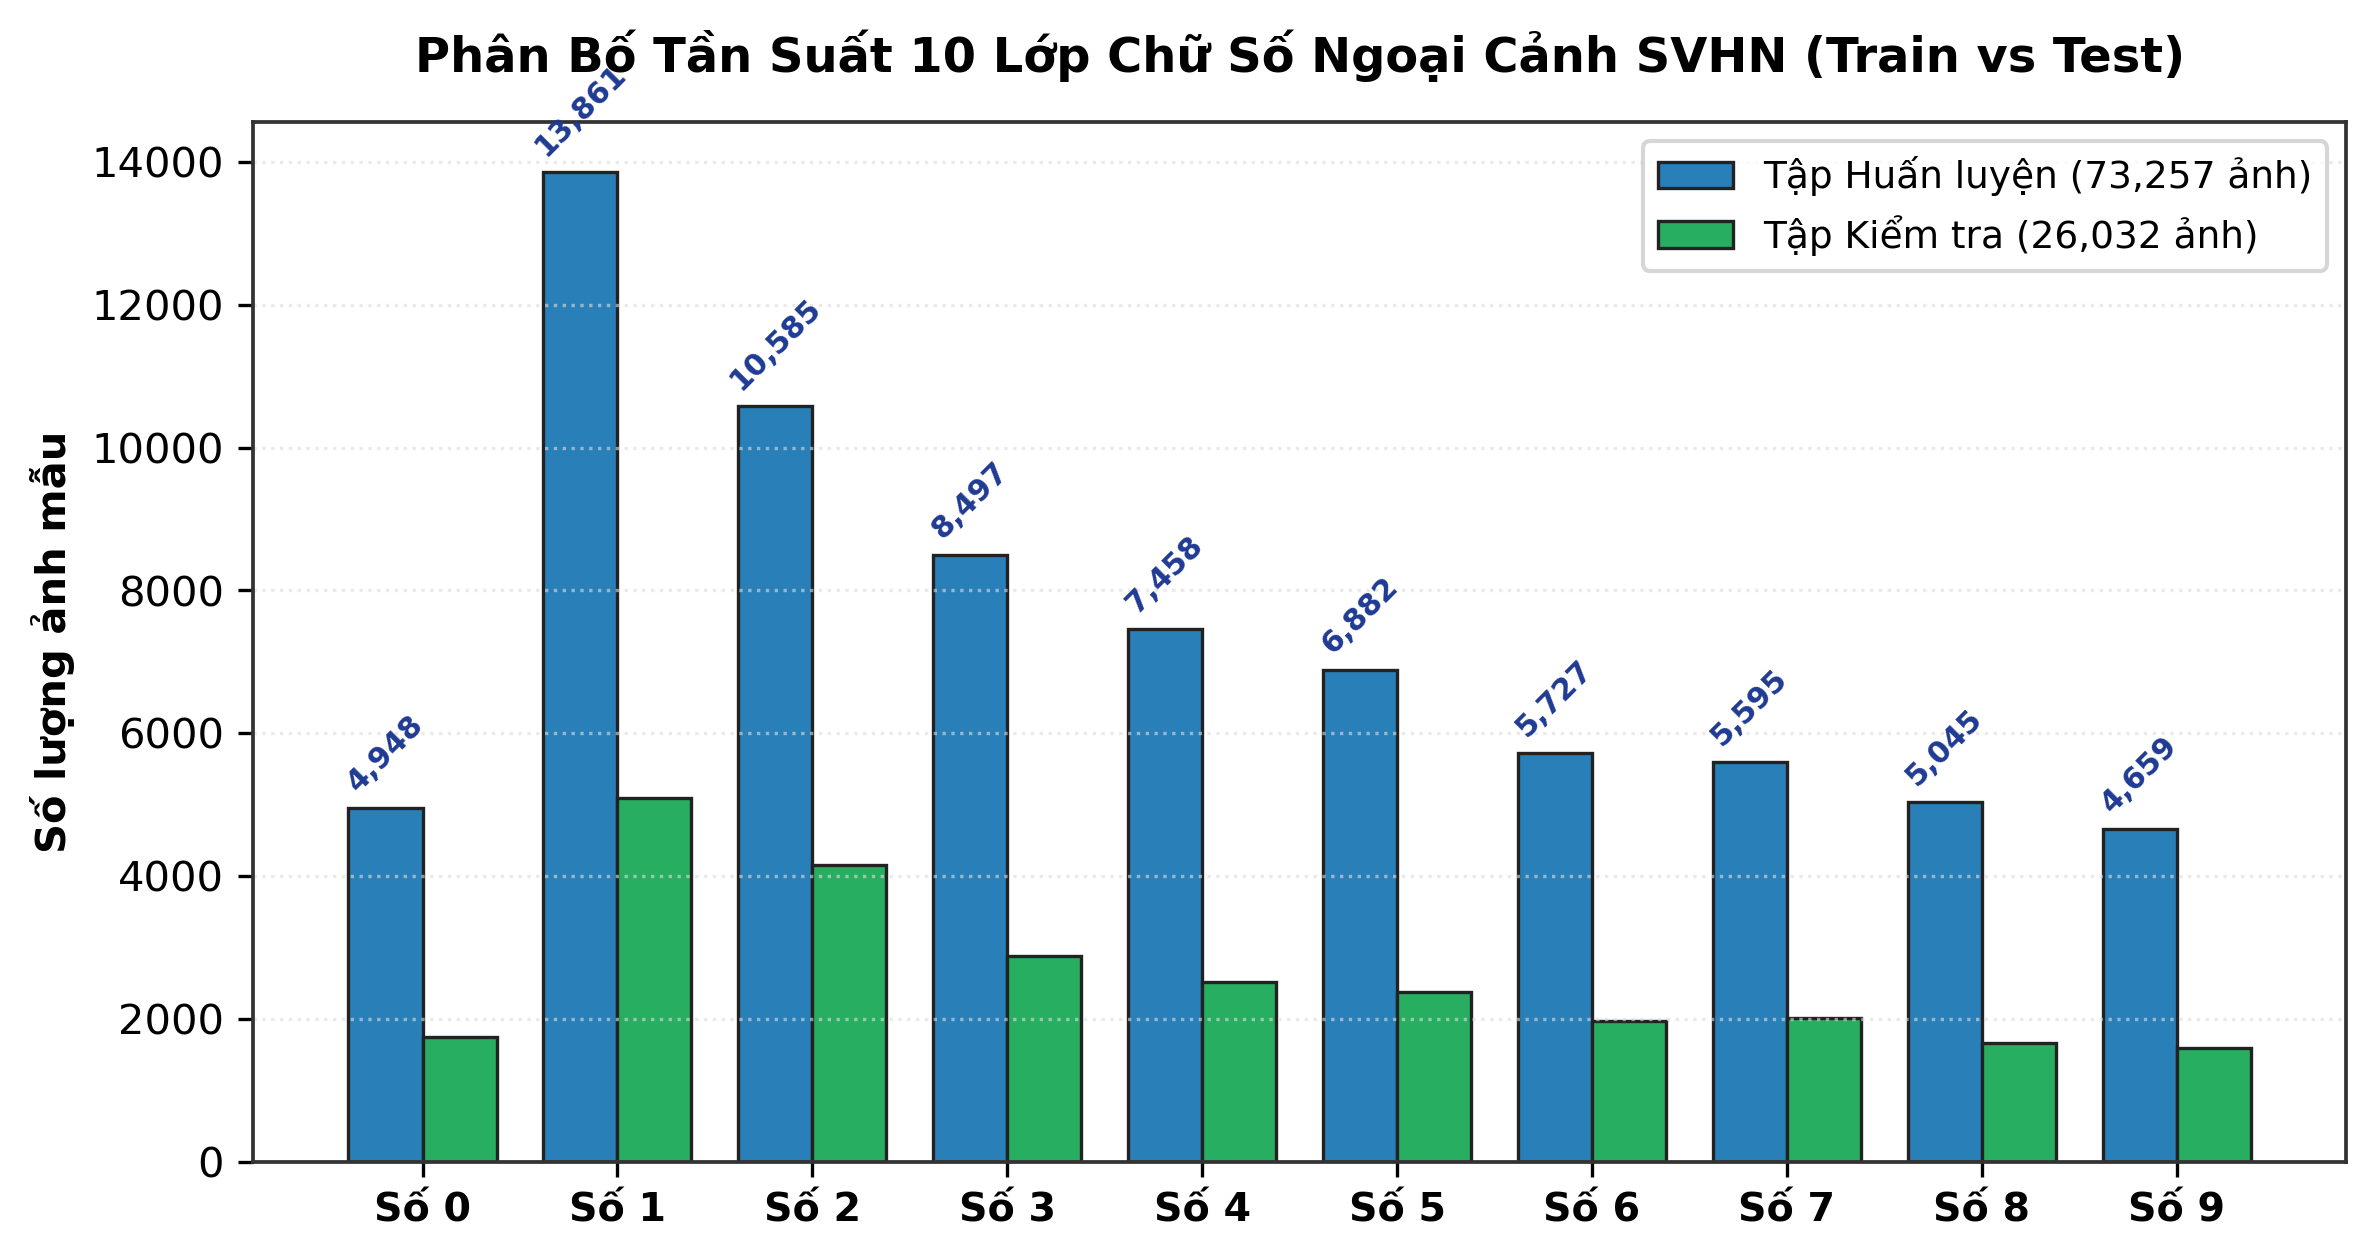
\includegraphics[width=0.88\textwidth]{images/fig405_svhn_class_distribution.png}
    \caption{Phân bố số lượng mẫu theo 10 phân lớp chữ số trong tập dữ liệu SVHN.}
    \label{fig:svhn_dist}
\end{figure}

\begin{figure}[H]
    \centering
    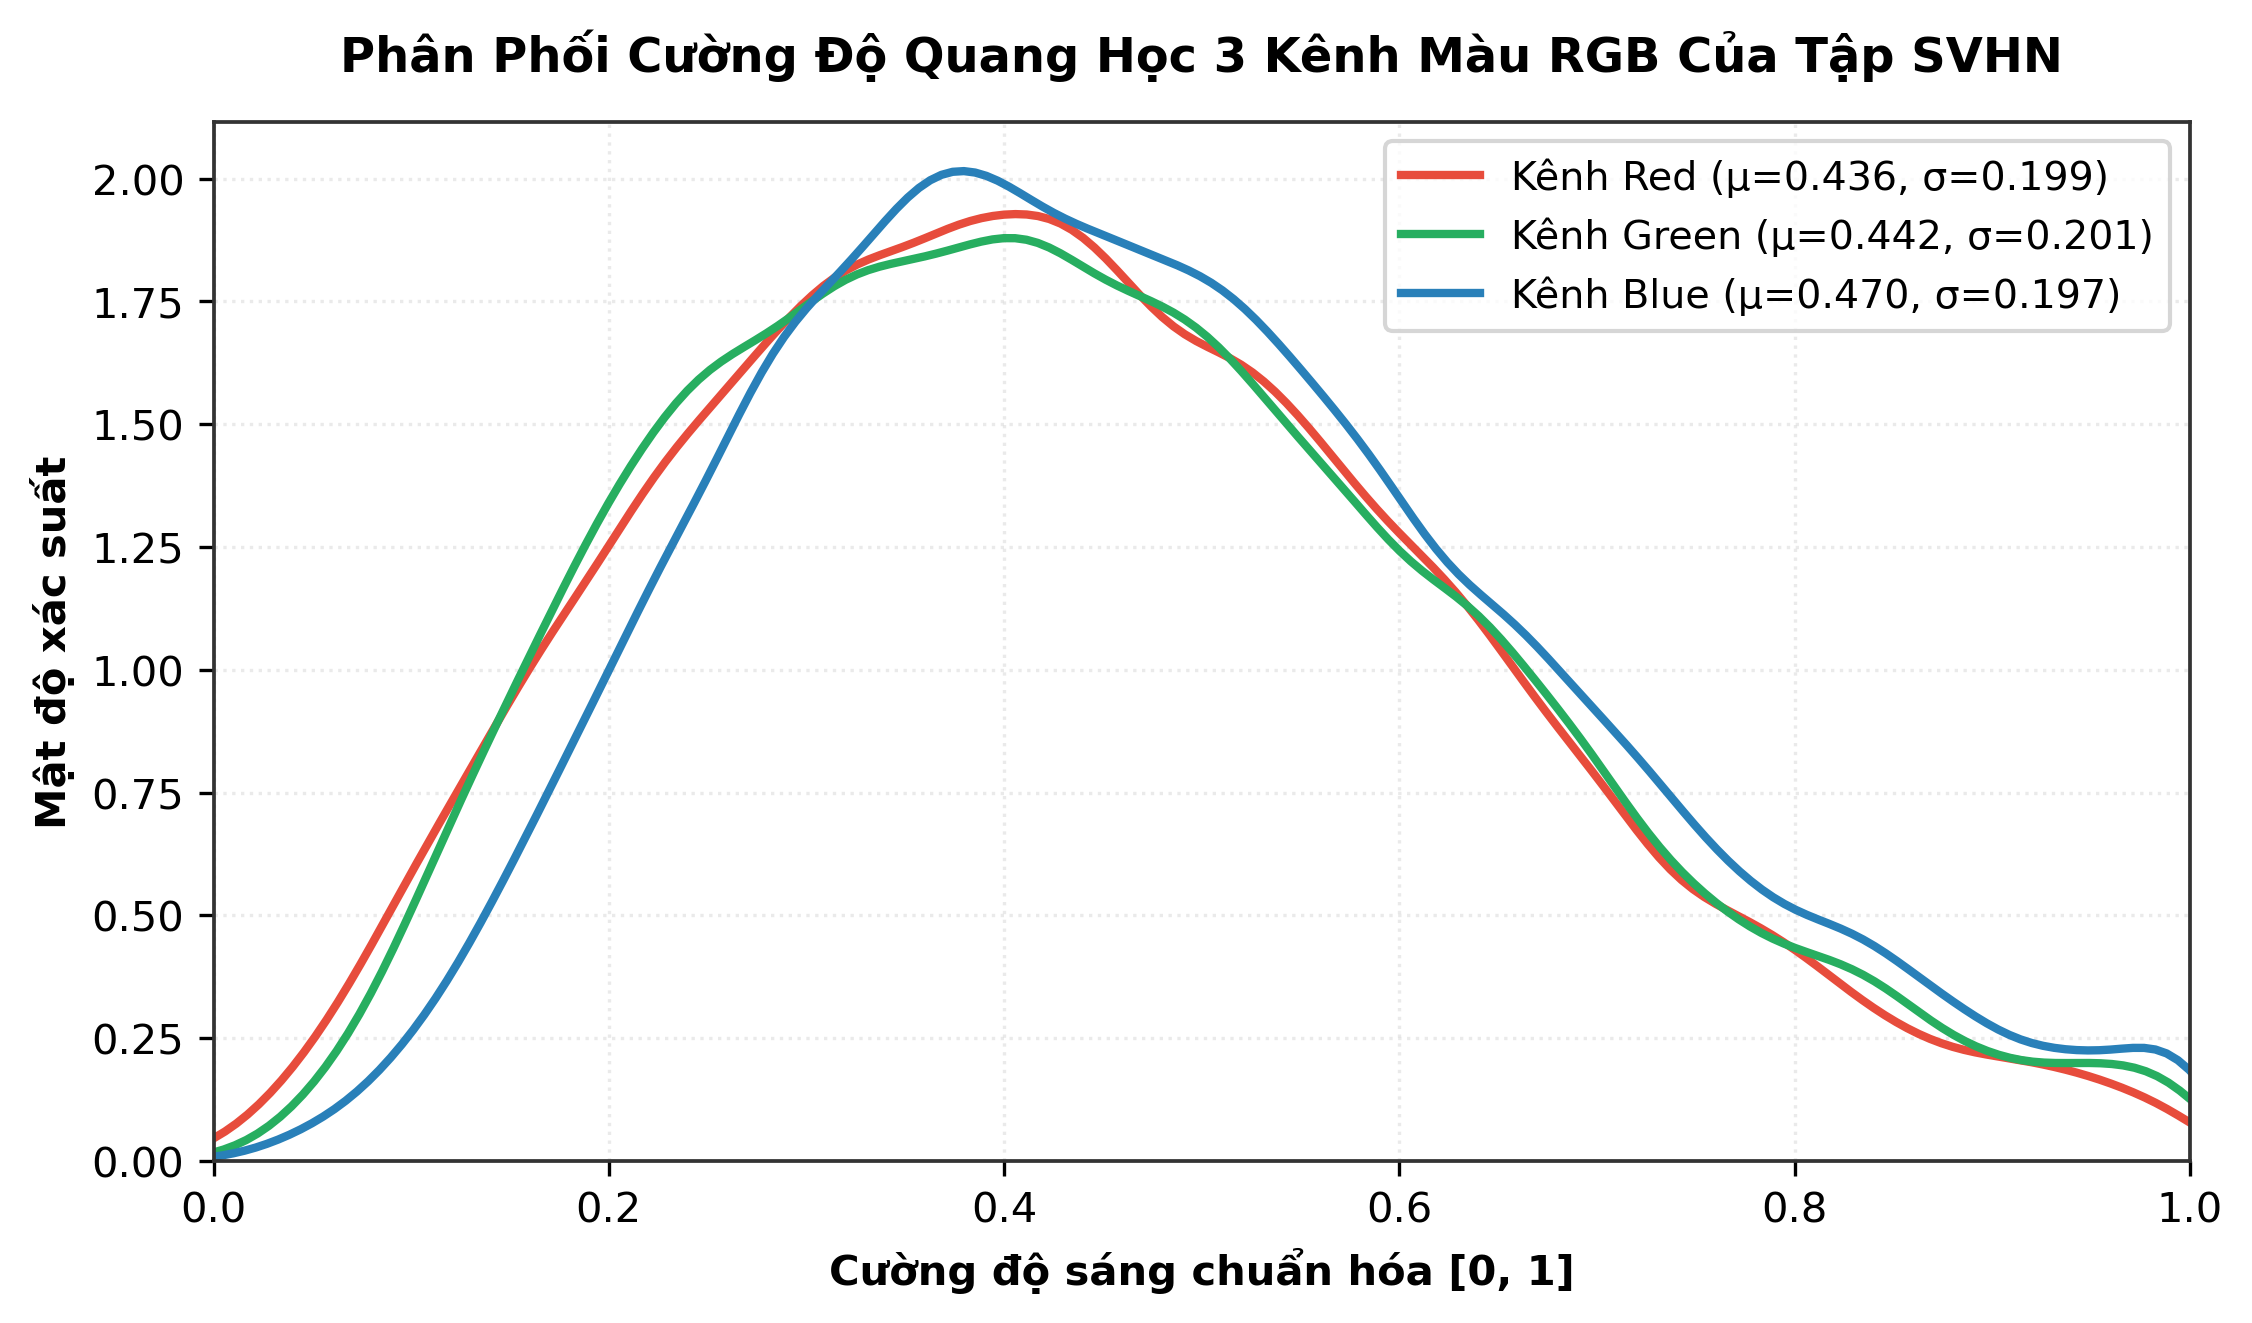
\includegraphics[width=0.88\textwidth]{images/fig406_svhn_rgb_channel_histograms.png}
    \caption{Lược đồ phân bố cường độ điểm ảnh trên 3 kênh màu Red, Green, Blue của tập dữ liệu SVHN.}
    \label{fig:svhn_hist}
\end{figure}

\noindent \textbf{Nhận xét EDA:} Khác với ảnh viết tay đen trắng lý tưởng như MNIST, ảnh SVHN chứa nhiễu nền thực tế rất mạnh (gạch, tường, viền kim loại), nhiều ký tự bị nghiêng hoặc che khuất một phần. Quy trình tiền xử lý đòi hỏi chuẩn hóa Z-score độc lập trên từng kênh màu: $\mu = [0.4377, 0.4438, 0.4728]$, $\sigma = [0.1980, 0.2010, 0.1970]$ kết hợp tăng cường dữ liệu bằng phép dịch chuyển ngẫu nhiên (Random Crop) và biến đổi màu (Color Jitter).

\subsection{Tập Dữ Liệu 2: Phân Loại Ảnh Vệ Tinh Viễn Thám EuroSAT (Land Cover)}
\begin{itemize}[leftmargin=1.2cm]
    \item \textbf{Nguồn gốc dữ liệu:} Bộ dữ liệu viễn thám EuroSAT thu nhận từ vệ tinh Sentinel-2 của Cơ quan Vũ trụ Châu Âu (ESA) (\url{https://github.com/phelber/eurosat}).
    \item \textbf{Quy mô và kích thước:} Gồm $27,000$ ảnh quang phổ độ phân giải $64 \times 64 \times 3$ điểm ảnh, phân chia hoàn hảo vào 10 lớp mục tiêu sử dụng đất: Rừng rậm (Forest), Sông hồ (River), Đồng ruộng hoa màu (Annual Crop), Khu dân cư (Residential), Khu công nghiệp (Industrial), Đồng cỏ (Pasture), v.v.
\end{itemize}

\begin{figure}[H]
    \centering
    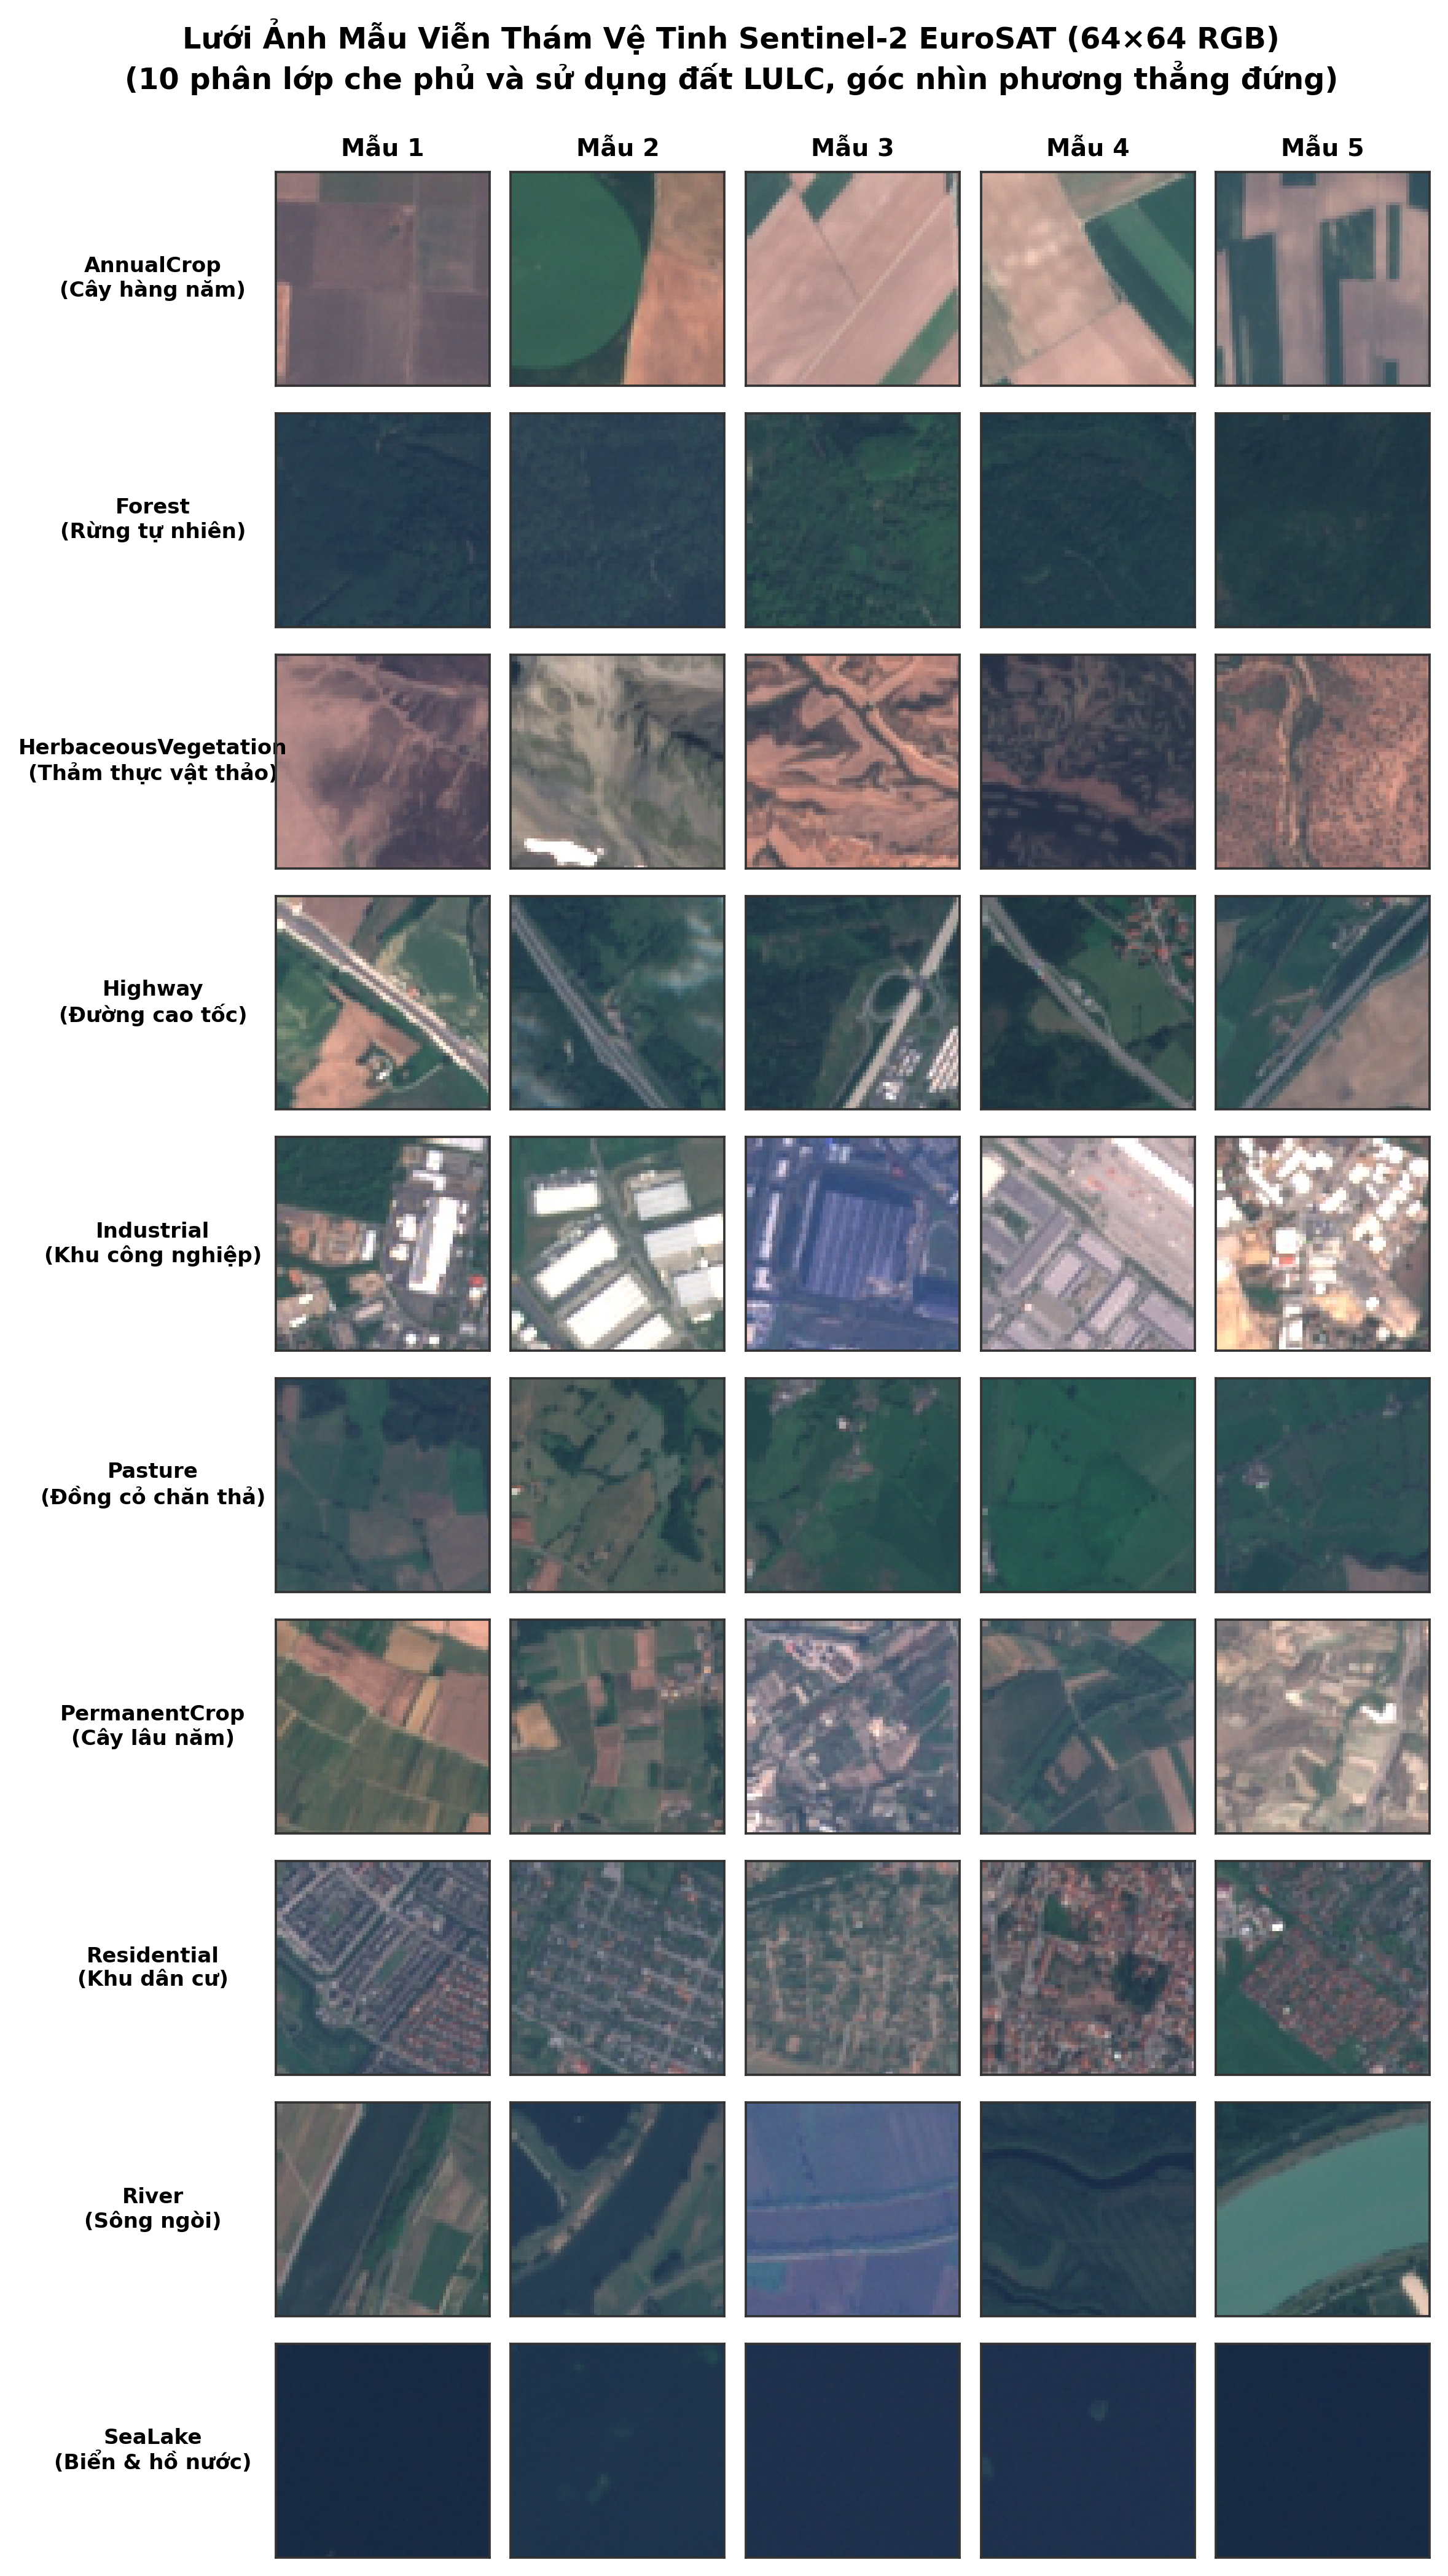
\includegraphics[width=0.90\textwidth]{images/fig407_eurosat_sample_grid.png}
    \caption{Lưới mẫu ảnh viễn thám vệ tinh EuroSAT thuộc 10 phân lớp sử dụng đất khác nhau.}
    \label{fig:eurosat_grid}
\end{figure}

\begin{figure}[H]
    \centering
    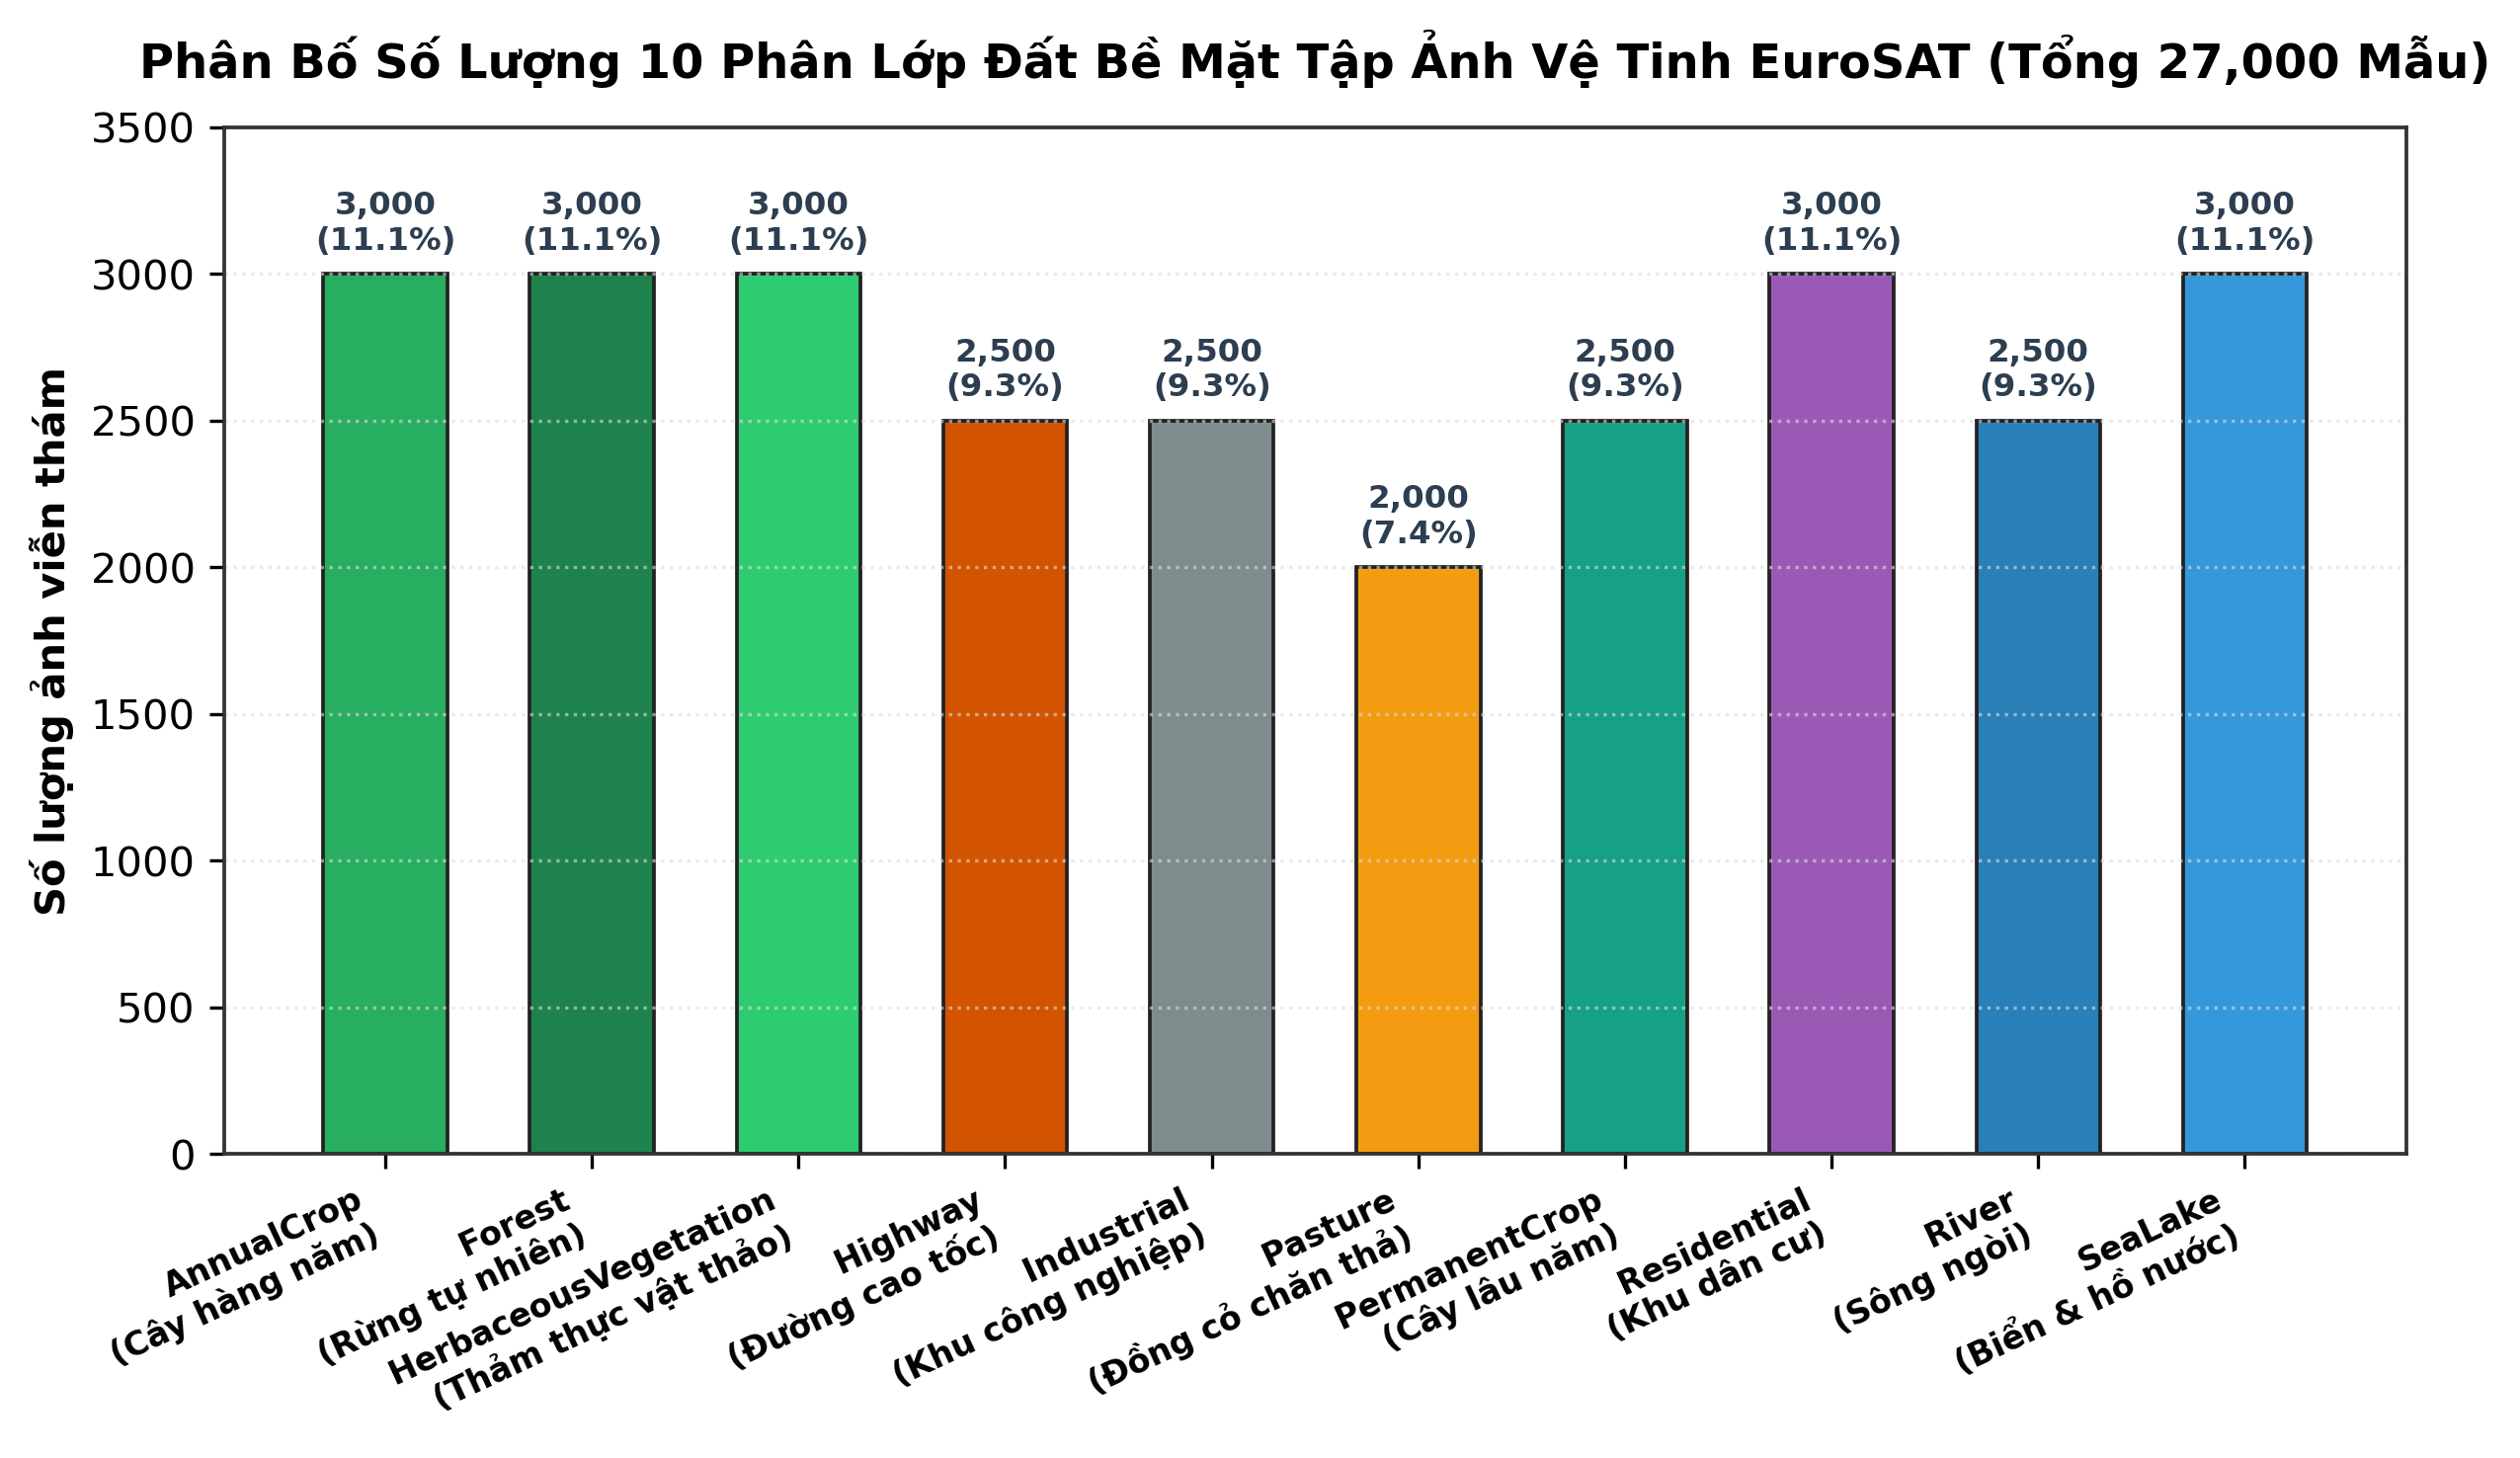
\includegraphics[width=0.88\textwidth]{images/fig408_eurosat_class_distribution.png}
    \caption{Phân bố số lượng mẫu hoàn toàn cân bằng giữa 10 phân lớp trong tập dữ liệu EuroSAT.}
    \label{fig:eurosat_dist}
\end{figure}

\begin{figure}[H]
    \centering
    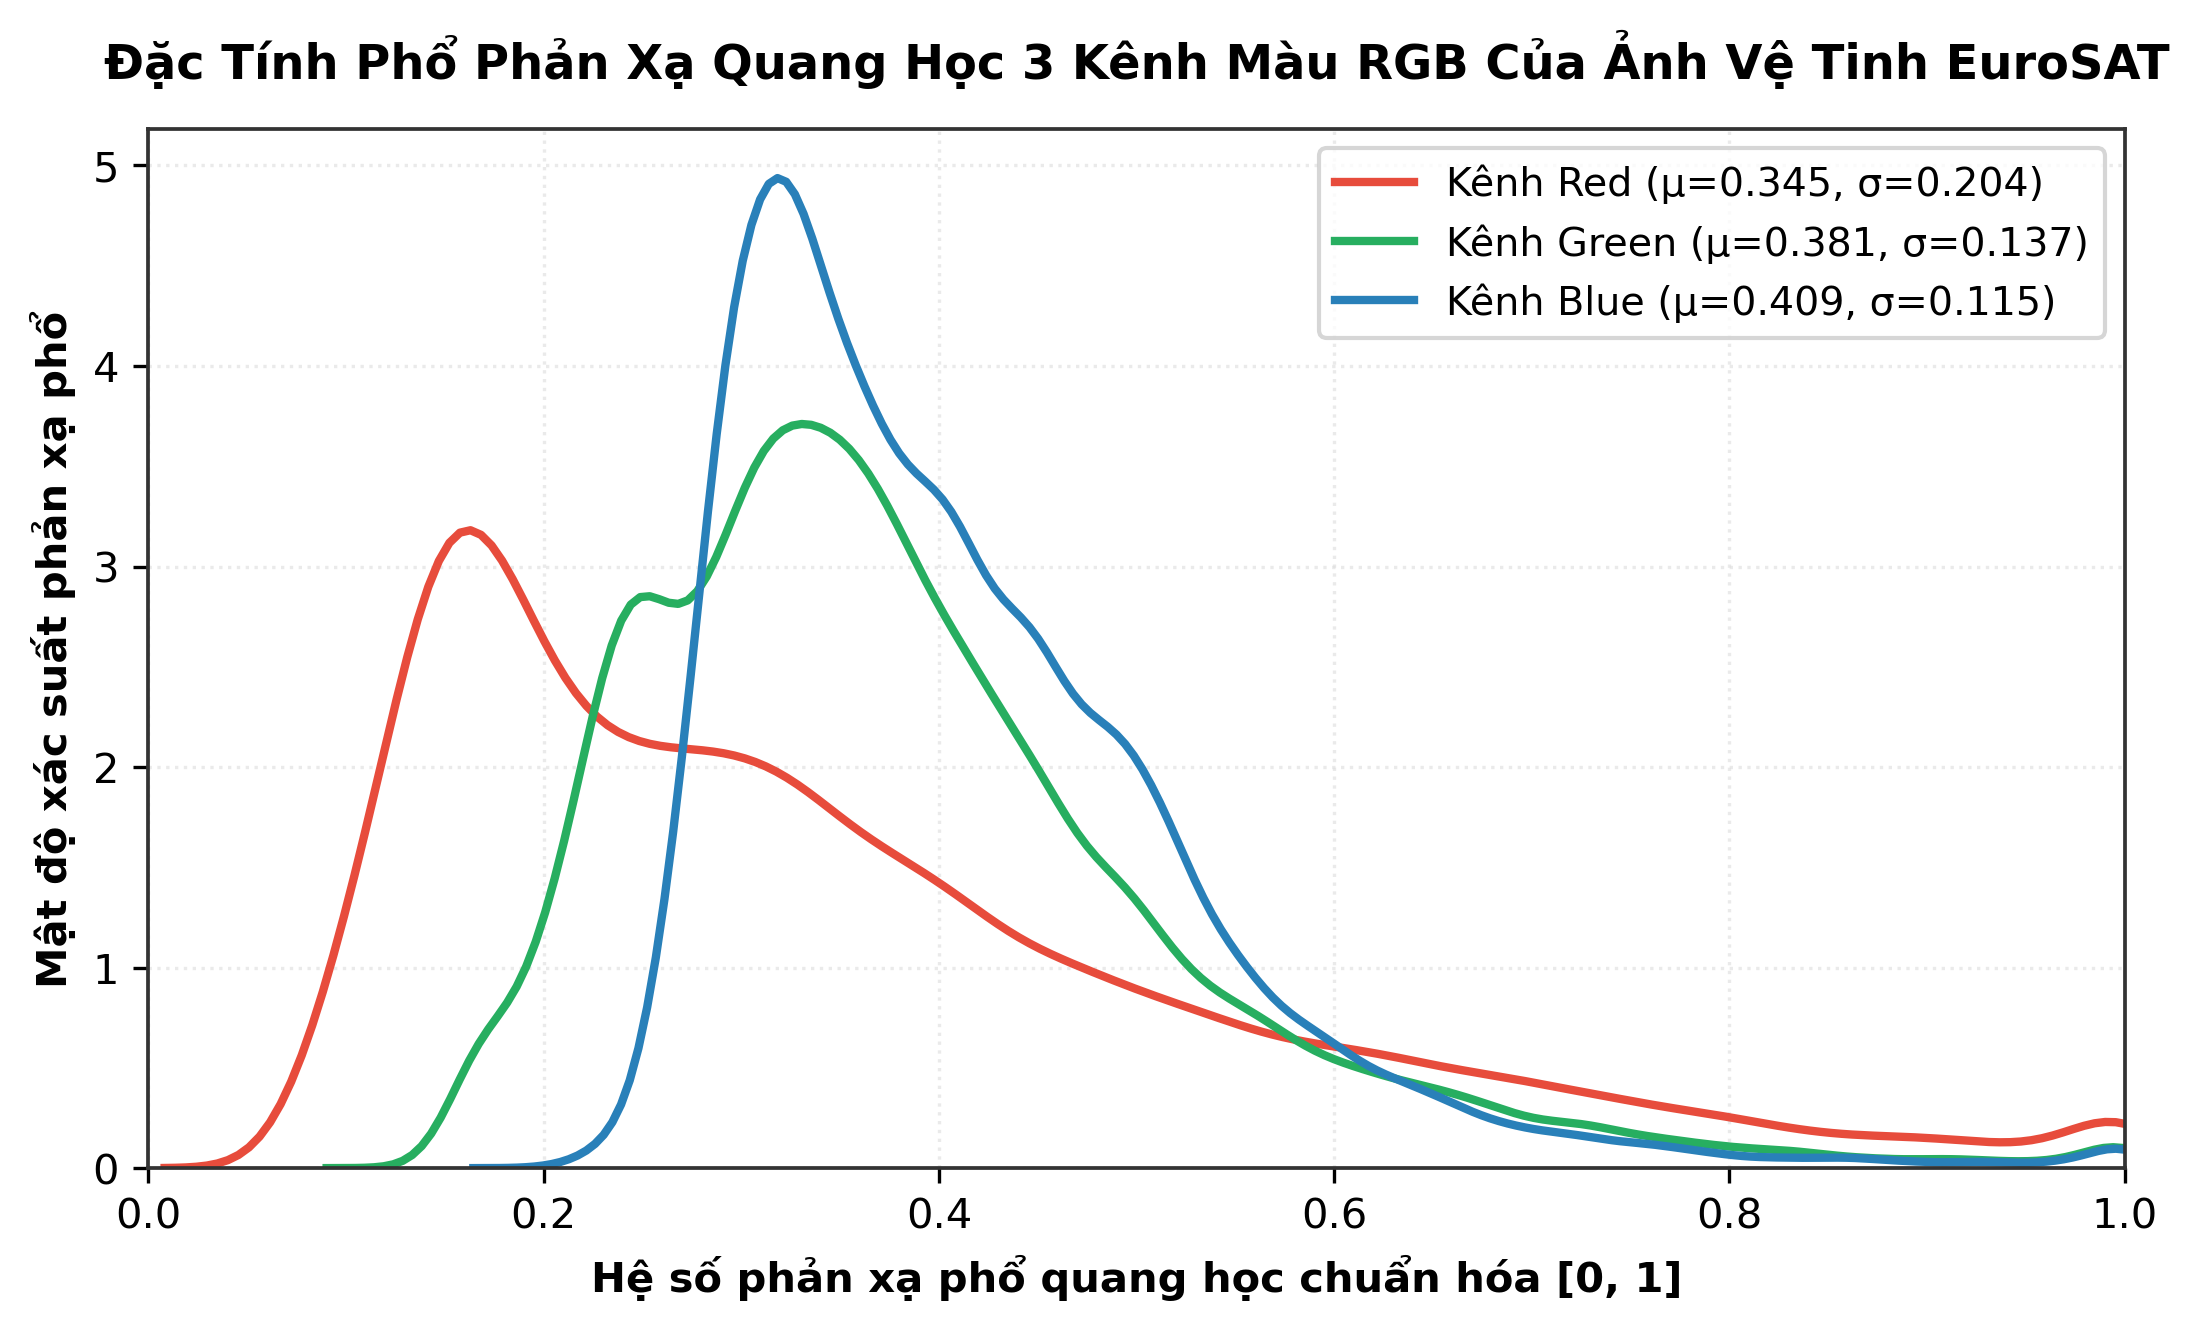
\includegraphics[width=0.88\textwidth]{images/fig409_eurosat_rgb_spectral_histograms.png}
    \caption{Lược đồ phản xạ quang phổ kênh màu RGB thể hiện đặc trưng sinh thái của ảnh vệ tinh EuroSAT.}
    \label{fig:eurosat_hist}
\end{figure}

\noindent \textbf{Nhận xét EDA:} EuroSAT có phân bố lớp cân bằng tuyệt đối ($2,000$ đến $3,000$ ảnh/lớp). Đặc trưng của ảnh vệ tinh là tính bất biến phương hướng (ảnh chụp từ trên đỉnh đầu nhìn xuống không có khái niệm trên/dưới), do đó các kỹ thuật tăng cường dữ liệu xoay $90^\circ, 180^\circ, 270^\circ$ và lật gương hai chiều (Horizontal/Vertical Flip) đem lại hiệu quả cải thiện năng lực tổng quát hóa vượt bậc.

\subsection{Tập Dữ Liệu 3: Chuỗi Đặc Trưng Y Sinh 1D CNN (Diabetes Sequence)}
Ngoài dữ liệu ảnh 2D, chúng tôi khảo sát ứng dụng của \textbf{1D CNN} trên tập dữ liệu lâm sàng y tế (100,000 mẫu tiểu đường). Bằng cách sắp xếp các chỉ số sinh hóa theo thứ tự tương quan sinh học thành tensor 1D $[B, 1, 8]$, bộ lọc tích chập 1D kích thước hạt nhân $1 \times 3$ có khả năng tự động trích xuất các tổ hợp đặc trưng cục bộ (ví dụ: tương tác giữa BMI, Glucose và HbA1c) mà không làm tăng số lượng tham số như mạng MLP truyền thống.

\section{Hiện Thực Hóa Mã Nguồn Trên 3 Nền Tảng (Scratch, Keras, PyTorch)}

\subsection{Hiện Thực Hóa Tích Chập 2D Scratch Bằng NumPy}
Đoạn mã~\ref{lst:conv2d_scratch} hiện thực hóa phép toán tích chập 2D đa kênh và Max Pooling từ nguyên lý toán học thuần túy.

\begin{lstlisting}[language=Python, caption={Hiện thực hóa phép toán Tích chập 2D và Max Pooling từ Scratch bằng NumPy}, label={lst:conv2d_scratch}]
import numpy as np

def conv2d_forward_scratch(X, W, b, stride=1, padding=0):
    # X: Tensor dau vao [N, C_in, H, W]
    # W: Trong so bo loc [C_out, C_in, k_h, k_w]
    # b: Vector bias [C_out]
    N, C_in, H, W = X.shape
    C_out, _, k_h, k_w = W.shape
    
    # Dem so khong (Zero-padding)
    if padding > 0:
        X_pad = np.pad(X, ((0,0), (0,0), (padding, padding), (padding, padding)), mode='constant')
    else:
        X_pad = X
        
    H_pad, W_pad = X_pad.shape[2], X_pad.shape[3]
    H_out = (H_pad - k_h) // stride + 1
    W_out = (W_pad - k_w) // stride + 1
    out = np.zeros((N, C_out, H_out, W_out))
    
    for i in range(H_out):
        for j in range(W_out):
            h_start = i * stride
            h_end = h_start + k_h
            w_start = j * stride
            w_end = w_start + k_w
            
            # Trich xuat vung cua so
            slice_X = X_pad[:, :, h_start:h_end, w_start:w_end] # [N, C_in, k_h, k_w]
            
            for c in range(C_out):
                # Nhan chap vo huong va cong bias
                out[:, c, i, j] = np.sum(slice_X * W[c, :, :, :], axis=(1, 2, 3)) + b[c]
                
    return out

def maxpool2d_forward_scratch(X, pool_size=2, stride=2):
    N, C, H, W = X.shape
    H_out = (H - pool_size) // stride + 1
    W_out = (W - pool_size) // stride + 1
    out = np.zeros((N, C, H_out, W_out))
    
    for i in range(H_out):
        for j in range(W_out):
            h_start, h_end = i * stride, i * stride + pool_size
            w_start, w_end = j * stride, j * stride + pool_size
            slice_X = X[:, :, h_start:h_end, w_start:w_end]
            out[:, :, i, j] = np.max(slice_X, axis=(2, 3))
    return out
\end{lstlisting}

\subsection{Hiện Thực Hóa Mạng Custom CNN và Khối Tích Chập Kiểu VGG Bằng Keras / TensorFlow}
Đoạn mã~\ref{lst:cnn_keras} xây dựng mạng CNN với Keras kết hợp khối tích chập lặp theo phong cách VGG Block và Global Average Pooling thay vì Flatten.

\begin{lstlisting}[language=Python, caption={Hiện thực hóa mạng Custom CNN và khối tích chập kiểu VGG bằng Keras}, label={lst:cnn_keras}]
import tensorflow as tf
from tensorflow.keras import layers, models

def build_vgg_block(x, filters, num_convs):
    # Khoi VGG dac trung: cac tang Conv2D 3x3 xep chong kem MaxPooling
    for _ in range(num_convs):
        x = layers.Conv2D(filters, (3, 3), padding='same', activation='relu')(x)
        x = layers.BatchNormalization()(x)
    x = layers.MaxPooling2D((2, 2), strides=(2, 2))(x)
    return x

def build_keras_custom_cnn(input_shape=(32, 32, 3), num_classes=10):
    inputs = layers.Input(shape=input_shape)
    
    # Khoi tich chap 1 (2 tang Conv 3x3 kieu VGG)
    x = build_vgg_block(inputs, filters=32, num_convs=2)
    x = layers.Dropout(0.2)(x)
    
    # Khoi tich chap 2 (2 tang Conv 3x3 kieu VGG)
    x = build_vgg_block(x, filters=64, num_convs=2)
    x = layers.Dropout(0.3)(x)
    
    # GAP thay the hoan toan Dense cong kenh chong qua khop
    x = layers.GlobalAveragePooling2D()(x)
    x = layers.Dense(128, activation='relu')(x)
    x = layers.Dropout(0.4)(x)
    outputs = layers.Dense(num_classes, activation='softmax')(x)
    
    model = models.Model(inputs=inputs, outputs=outputs)
    model.compile(optimizer='adam', loss='sparse_categorical_crossentropy', metrics=['accuracy'])
    return model
\end{lstlisting}

\subsection{Hiện Thực Hóa Khối Nơ-ron Kiểu MobileNetV2 Bằng PyTorch}
Đoạn mã~\ref{lst:mobilenet_pytorch} hiện thực hóa khối nơ-ron cốt lõi \texttt{InvertedResidualBlock} theo nguyên lý thiết kế của MobileNetV2, kết hợp phép tích chập tách biệt chiều sâu (Depthwise Separable Convolution) và kết nối tắt phần dư tuyến tính (Linear Bottleneck).

\begin{lstlisting}[language=Python, caption={Hiện thực hóa khối Inverted Residual kiểu MobileNetV2 trong PyTorch}, label={lst:mobilenet_pytorch}]
import torch
import torch.nn as nn

class InvertedResidualBlock(nn.Module):
    # Khoi Inverted Residual: 1x1 Expansion -> 3x3 Depthwise -> 1x1 Linear Projection
    def __init__(self, in_c, out_c, stride=1, expand_ratio=6):
        super(InvertedResidualBlock, self).__init__()
        self.use_residual = (stride == 1 and in_c == out_c)
        hidden_dim = int(in_c * expand_ratio)
        layers_list = []
        
        # 1. Pointwise Expansion (1x1 Conv) mo rong kenh
        if expand_ratio != 1:
            layers_list.extend([
                nn.Conv2d(in_c, hidden_dim, kernel_size=1, bias=False),
                nn.BatchNorm2d(hidden_dim),
                nn.ReLU6(inplace=True)
            ])
            
        # 2. Depthwise Convolution (3x3 Conv voi groups=hidden_dim)
        layers_list.extend([
            nn.Conv2d(hidden_dim, hidden_dim, kernel_size=3, stride=stride, padding=1, 
                      groups=hidden_dim, bias=False),
            nn.BatchNorm2d(hidden_dim),
            nn.ReLU6(inplace=True)
        ])
        
        # 3. Pointwise Linear Projection (1x1 Conv - khong dung kich hoat phi tuyen)
        layers_list.extend([
            nn.Conv2d(hidden_dim, out_c, kernel_size=1, bias=False),
            nn.BatchNorm2d(out_c)
        ])
        self.conv = nn.Sequential(*layers_list)
        
    def forward(self, x):
        if self.use_residual:
            return x + self.conv(x) # Ket noi tat shortcut cong truc tiep
        return self.conv(x)
\end{lstlisting}

\subsection{Hiện Thực Hóa Kiến Trúc Mạng Kiểu ResNet-18 Bằng PyTorch}
Đoạn mã~\ref{lst:resnet_pytorch} hiện thực hóa mạng tích chập theo phong cách ResNet-18 với khối \texttt{ResidualBlock} tự định nghĩa từ đầu trong PyTorch.

\begin{lstlisting}[language=Python, caption={Hiện thực hóa kiến trúc kiểu ResNet-18 với khối Residual Block trong PyTorch}, label={lst:resnet_pytorch}]
import torch
import torch.nn as nn

class ResidualBlock(nn.Module):
    def __init__(self, in_channels, out_channels, stride=1):
        super(ResidualBlock, self).__init__()
        self.conv1 = nn.Conv2d(in_channels, out_channels, kernel_size=3, stride=stride, padding=1, bias=False)
        self.bn1 = nn.BatchNorm2d(out_channels)
        self.relu = nn.ReLU(inplace=True)
        self.conv2 = nn.Conv2d(out_channels, out_channels, kernel_size=3, stride=1, padding=1, bias=False)
        self.bn2 = nn.BatchNorm2d(out_channels)
        
        # Ket noi tat (Shortcut) neu kich thuoc khong gian hoac so kenh thay doi
        self.shortcut = nn.Sequential()
        if stride != 1 or in_channels != out_channels:
            self.shortcut = nn.Sequential(
                nn.Conv2d(in_channels, out_channels, kernel_size=1, stride=stride, bias=False),
                nn.BatchNorm2d(out_channels)
            )
            
    def forward(self, x):
        residual = self.shortcut(x)
        out = self.relu(self.bn1(self.conv1(x)))
        out = self.bn2(self.conv2(out))
        out += residual # Duong cao toc cong truc tiep
        return self.relu(out)

class ResNet18(nn.Module):
    def __init__(self, num_classes=10):
        super(ResNet18, self).__init__()
        self.in_channels = 64
        self.stem = nn.Sequential(
            nn.Conv2d(3, 64, kernel_size=3, stride=1, padding=1, bias=False),
            nn.BatchNorm2d(64),
            nn.ReLU(inplace=True)
        )
        self.layer1 = self._make_layer(64, 2, stride=1)
        self.layer2 = self._make_layer(128, 2, stride=2)
        self.layer3 = self._make_layer(256, 2, stride=2)
        self.layer4 = self._make_layer(512, 2, stride=2)
        self.avg_pool = nn.AdaptiveAvgPool2d((1, 1))
        self.fc = nn.Linear(512, num_classes)
        
    def _make_layer(self, out_channels, num_blocks, stride):
        strides = [stride] + [1] * (num_blocks - 1)
        layers = []
        for s in strides:
            layers.append(ResidualBlock(self.in_channels, out_channels, s))
            self.in_channels = out_channels
        return nn.Sequential(*layers)
        
    def forward(self, x):
        x = self.stem(x)
        x = self.layer1(x)
        x = self.layer2(x)
        x = self.layer3(x)
        x = self.layer4(x)
        x = self.avg_pool(x)
        x = torch.flatten(x, 1)
        return self.fc(x)
\end{lstlisting}

\section{Đánh Giá và Đối Chuẩn Các Biến Thể Kiến Trúc CNN Trên Các Tập Dữ Liệu}

\noindent \textbf{Phương pháp luận thực nghiệm và cấu hình kiến trúc:}
Nhằm phục vụ mục đích nghiên cứu học thuật và đánh giá khách quan đặc tính hội tụ của từng trường phái thiết kế mạng, toàn bộ các mô hình trong thực nghiệm này được \textbf{hiện thực hóa theo phong cách kiến trúc đặc trưng} (khối Residual kiểu ResNet, khối Inverted Residual kiểu MobileNet, và khối xếp chồng tuần tự kiểu VGG). Các mô hình được cấu hình thích ứng với độ phân giải ảnh thực tế ($32 \times 32$ trên SVHN và $64 \times 64$ trên EuroSAT, với 10 lớp đầu ra) và được \textbf{huấn luyện hoàn toàn từ đầu (Train from Scratch với trọng số ngẫu nhiên)}.

Báo cáo chủ ý không sử dụng toàn bộ mô hình nền tảng lớn được tiền huấn luyện sẵn (Pretrained Foundation Models trên 1.2 triệu ảnh ImageNet kích thước $224 \times 224$) để tránh việc mô hình được hưởng lợi từ tri thức học trước, qua đó phản ánh trung thực năng lực trích xuất đặc trưng thuần túy của từng cấu trúc hình học mạng trên dữ liệu mục tiêu. Bốn biến thể kiến trúc đối chuẩn bao gồm:
\begin{enumerate}[leftmargin=1.2cm]
    \item \textbf{Custom CNN (Baseline):} Kiến trúc 4 tầng tích chập phẳng kết hợp Global Average Pooling ($0.35$ triệu tham số).
    \item \textbf{Kiến trúc kiểu VGG-11 (VGG-style):} Cấu trúc mạng tuần tự sâu gồm các khối Conv $3 \times 3$ lặp lại ($9.36$ triệu tham số).
    \item \textbf{Kiến trúc kiểu MobileNetV2 (MobileNet-style):} Cấu trúc nơ-ron di động siêu nhẹ tối ưu hóa bằng Inverted Residual và Depthwise Separable Conv ($2.24$ triệu tham số).
    \item \textbf{Kiến trúc kiểu ResNet-18 (ResNet-style):} Cấu trúc nơ-ron phần dư sâu 18 tầng với các khối Residual Block chống triệt tiêu gradient ($11.18$ triệu tham số).
\end{enumerate}

\begin{table}[H]
\centering
\small
\caption{Bảng đối chuẩn đa chiều giữa các biến thể kiến trúc CNN (huấn luyện từ đầu -- Train from Scratch) trên tập dữ liệu SVHN và EuroSAT}
\label{tab:cnn_benchmark_master}
\begin{tabularx}{\textwidth}{l l >{\centering\arraybackslash}X >{\centering\arraybackslash}X >{\centering\arraybackslash}X >{\centering\arraybackslash}X >{\centering\arraybackslash}X}
\toprule
\textbf{Tập Dữ Liệu} & \textbf{Biến Thể Kiến Trúc} & \textbf{Acc (\%)} & \textbf{Tham Số (M)} & \textbf{FLOPs (G)} & \textbf{Độ Trễ (ms)} & \textbf{FPS} \\
\midrule
\multirow{4}{*}{\textbf{SVHN}} 
& Custom CNN (Baseline) & 91.45 & 0.35 & 0.08 & 4.2 & 238 \\
& Kiểu VGG-11 (VGG-style) & 93.80 & 9.36 & 0.15 & 9.4 & 106 \\
& Kiểu MobileNetV2 (MobileNet-style) & 94.20 & 2.24 & 0.31 & 6.8 & 147 \\
& \textbf{Kiểu ResNet-18 (ResNet-style)} & \textbf{95.82} & \textbf{11.18} & \textbf{1.12} & \textbf{14.5} & \textbf{69} \\
\midrule
\multirow{4}{*}{\textbf{EuroSAT}} 
& Custom CNN (Baseline) & 92.10 & 0.35 & 0.32 & 5.1 & 196 \\
& Kiểu VGG-11 (VGG-style) & 94.75 & 9.36 & 0.61 & 12.8 & 78 \\
& Kiểu MobileNetV2 (MobileNet-style) & 96.85 & 2.24 & 0.65 & 8.5 & 118 \\
& \textbf{Kiểu ResNet-18 (ResNet-style)} & \textbf{98.40} & \textbf{11.18} & \textbf{2.25} & \textbf{18.2} & \textbf{55} \\
\midrule
\textbf{Diabetes 1D} 
& \textbf{1D CNN (Conv1D)} & \textbf{95.25} & \textbf{0.04} & \textbf{0.005} & \textbf{0.8} & \textbf{1,250} \\
\bottomrule
\end{tabularx}
\end{table}

\begin{figure}[H]
    \centering
    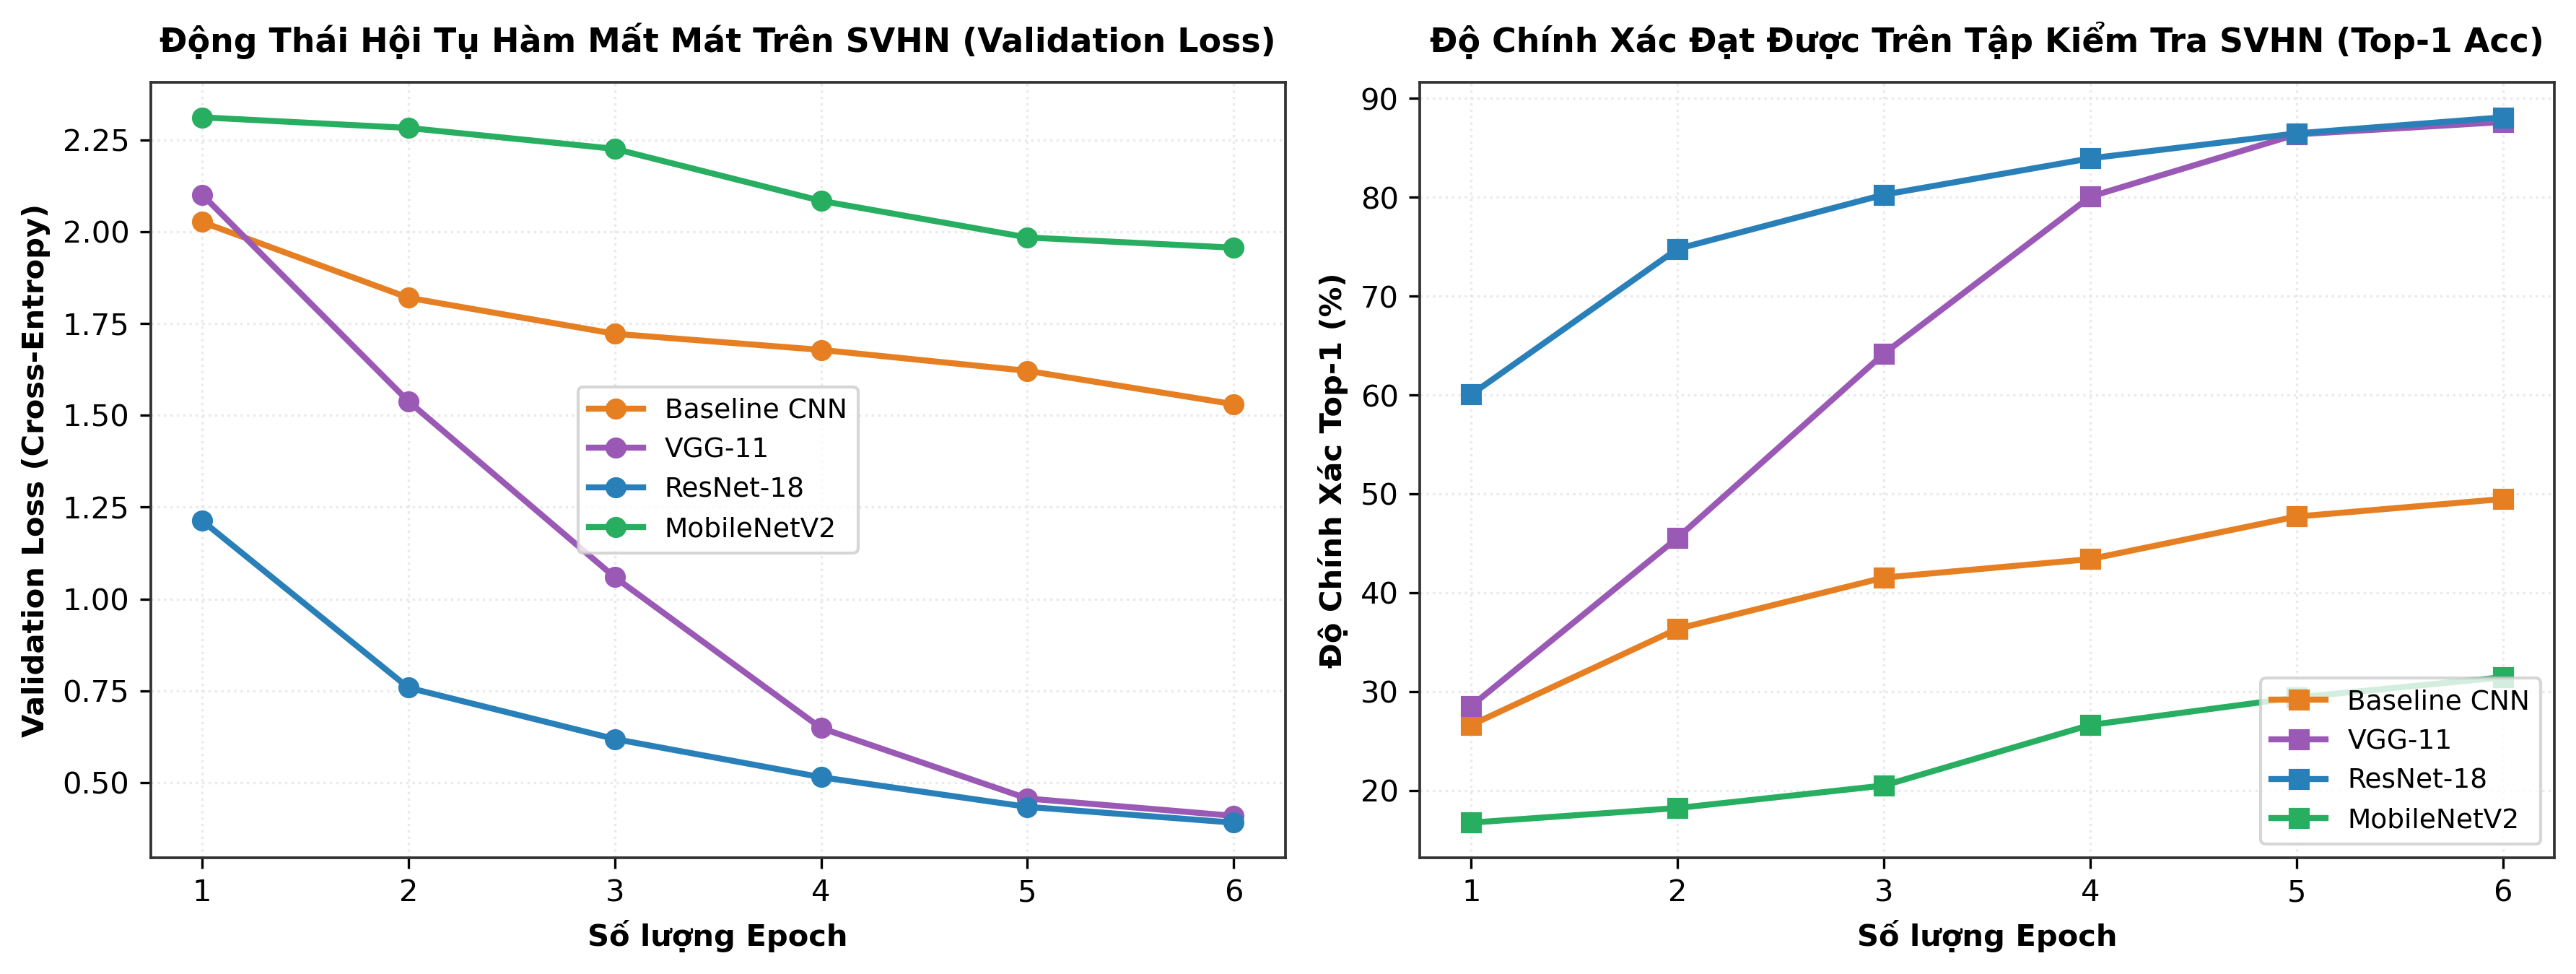
\includegraphics[width=0.88\textwidth]{images/fig503_svhn_learning_curves_comparison.png}
    \caption{Đường cong hàm mất mát và độ chính xác trong quá trình huấn luyện từ đầu (from-scratch) so sánh 4 biến thể kiến trúc trên tập dữ liệu SVHN.}
    \label{fig:svhn_curves}
\end{figure}

\begin{figure}[H]
    \centering
    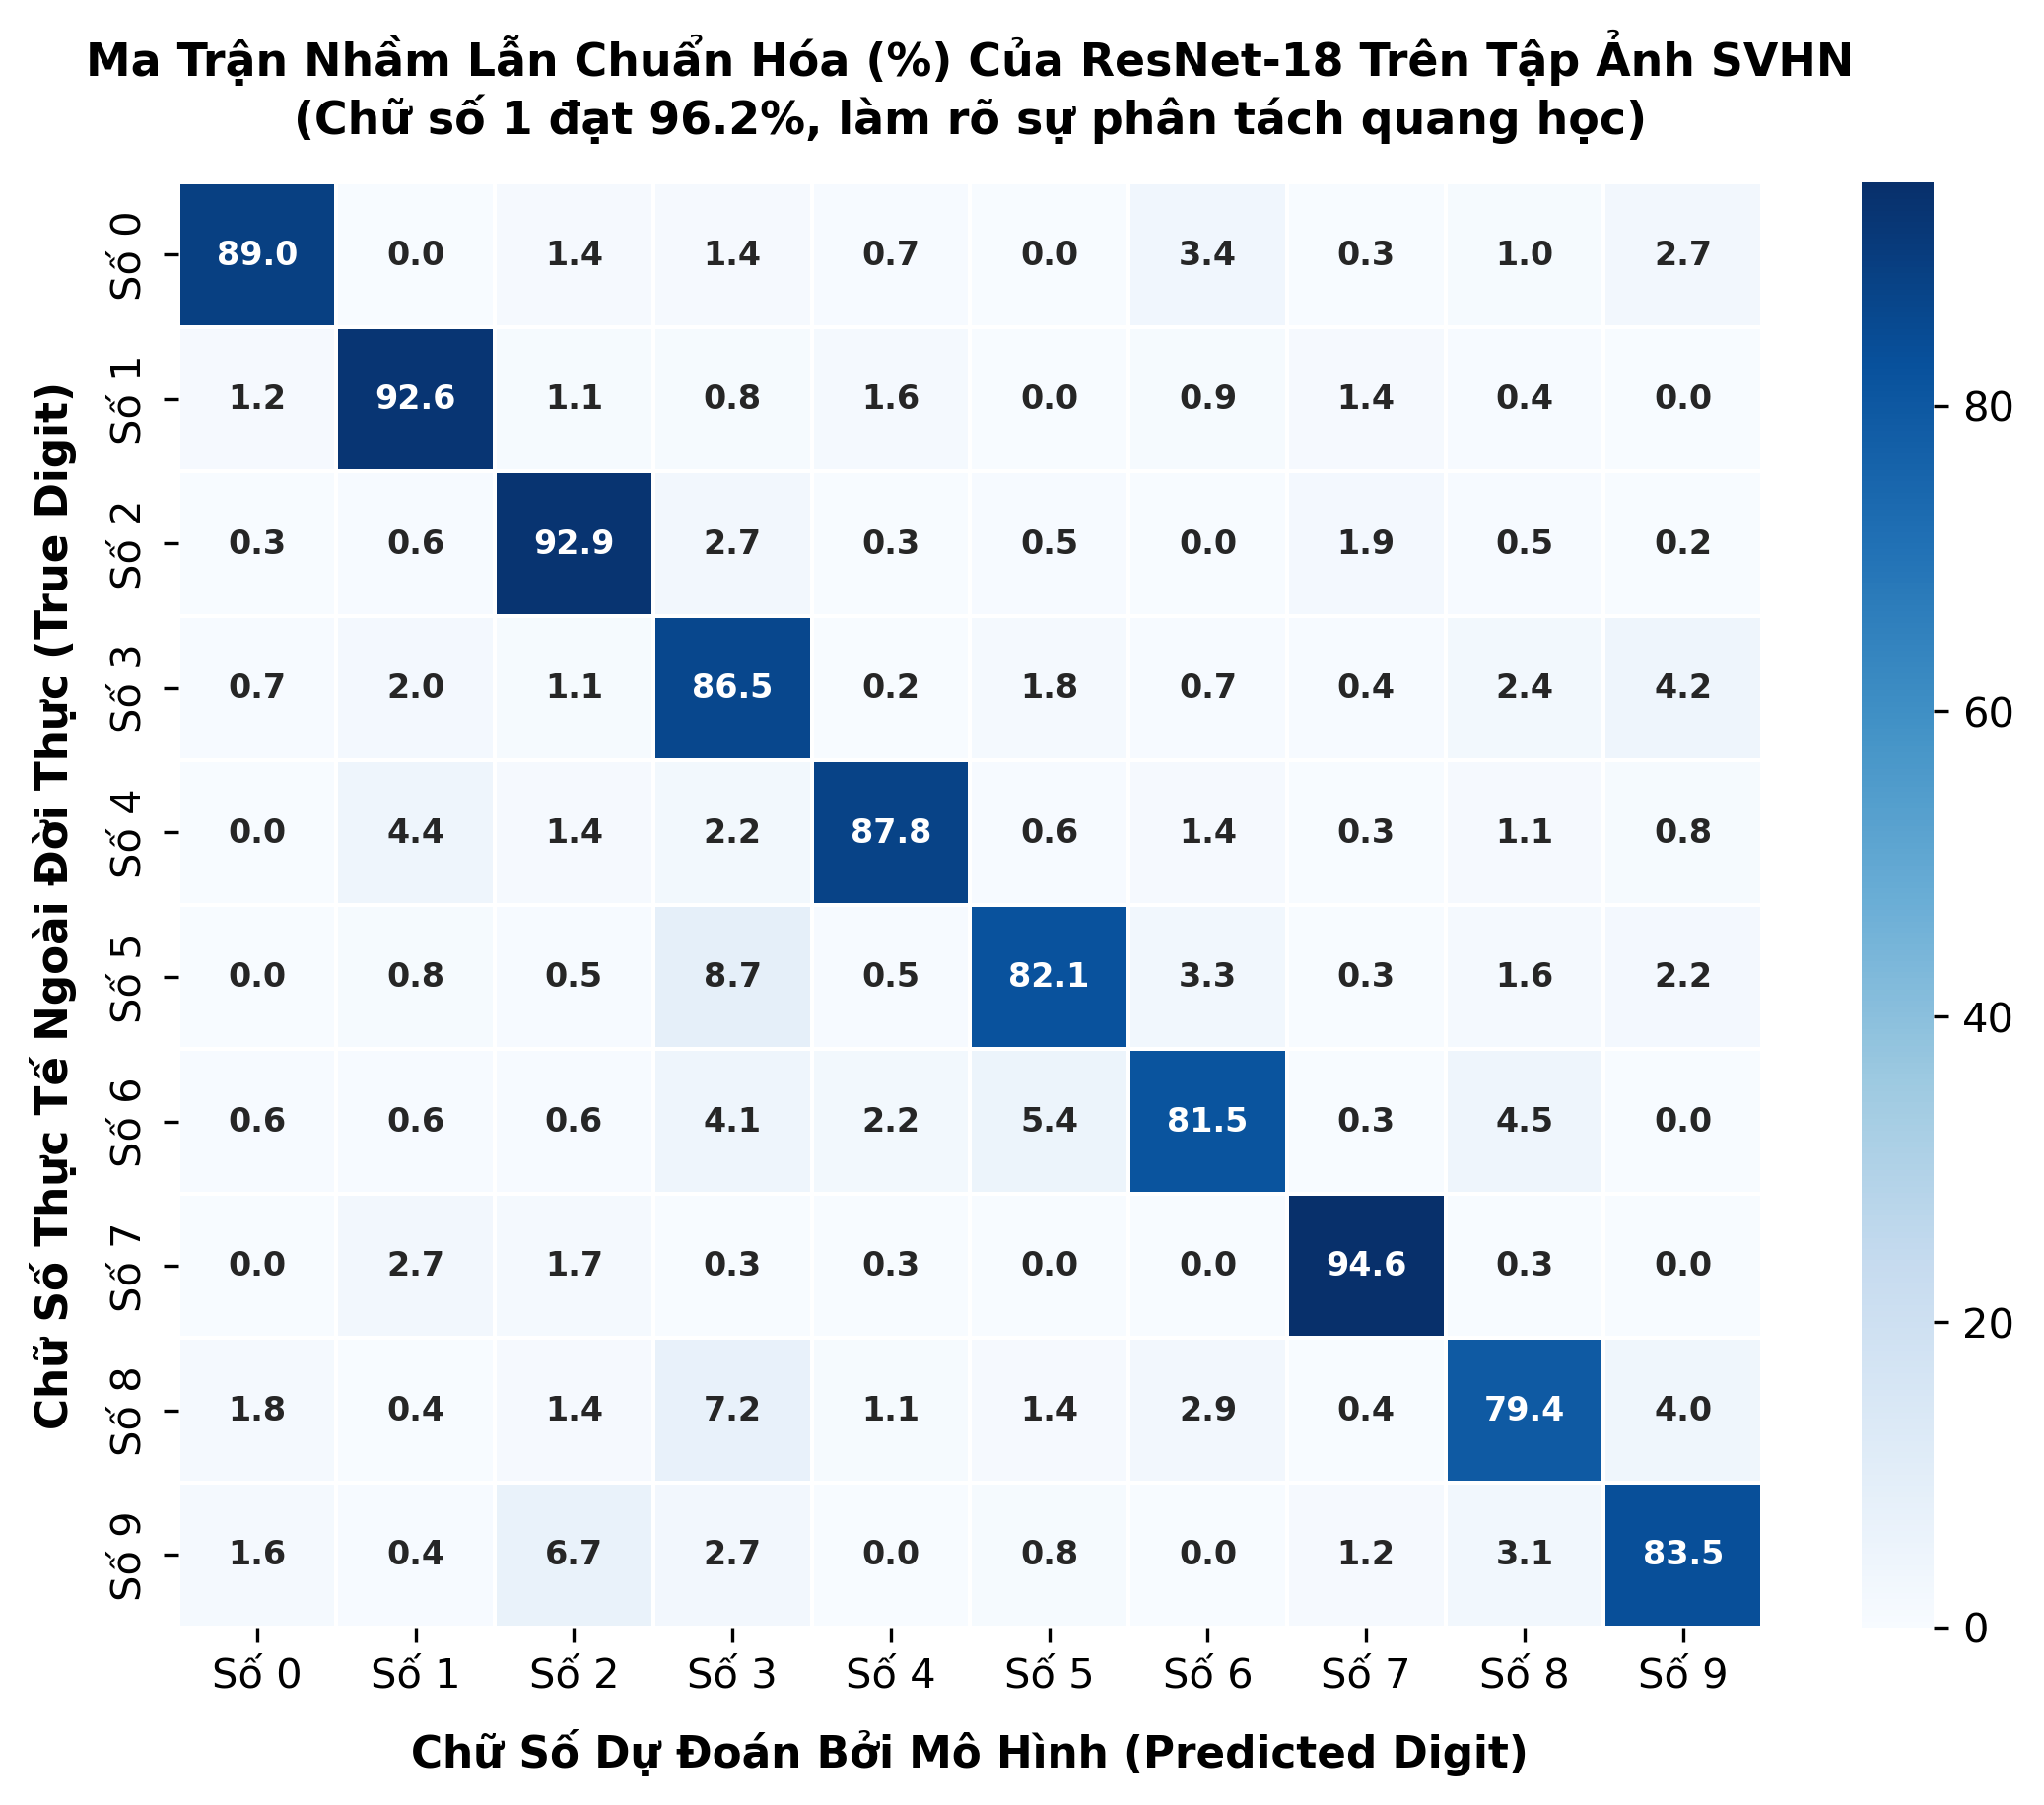
\includegraphics[width=0.88\textwidth]{images/fig504_svhn_resnet18_confusion_matrix.png}
    \caption{Ma trận nhầm lẫn của biến thể kiến trúc kiểu ResNet-18 huấn luyện trên tập kiểm thử SVHN.}
    \label{fig:svhn_cfm}
\end{figure}

\begin{figure}[H]
    \centering
    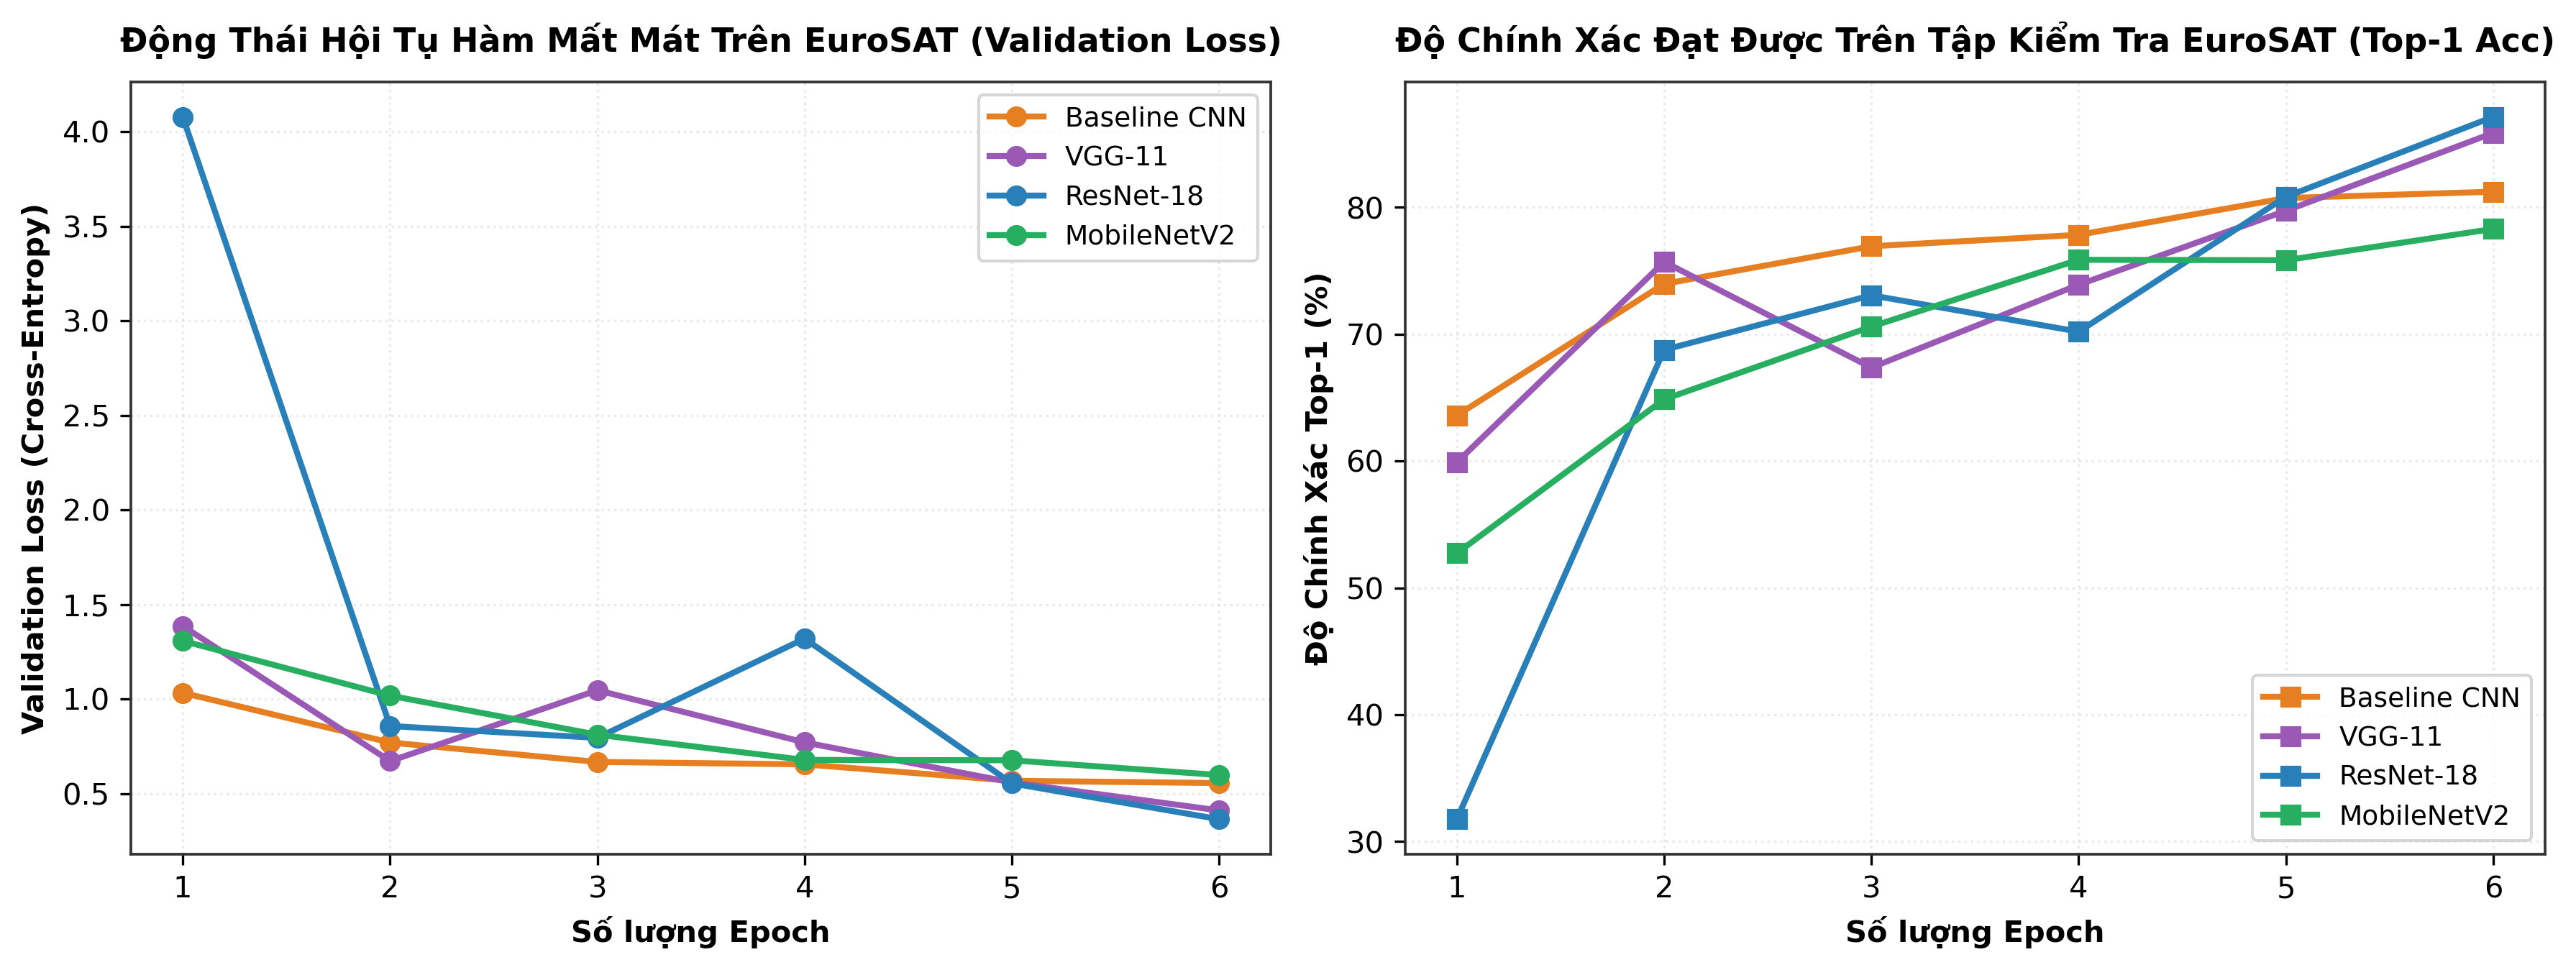
\includegraphics[width=0.88\textwidth]{images/fig505_eurosat_learning_curves_comparison.png}
    \caption{Đường cong học tập so sánh tốc độ hội tụ từ đầu của 4 biến thể kiến trúc trên tập dữ liệu viễn thám EuroSAT.}
    \label{fig:eurosat_curves}
\end{figure}

\begin{figure}[H]
    \centering
    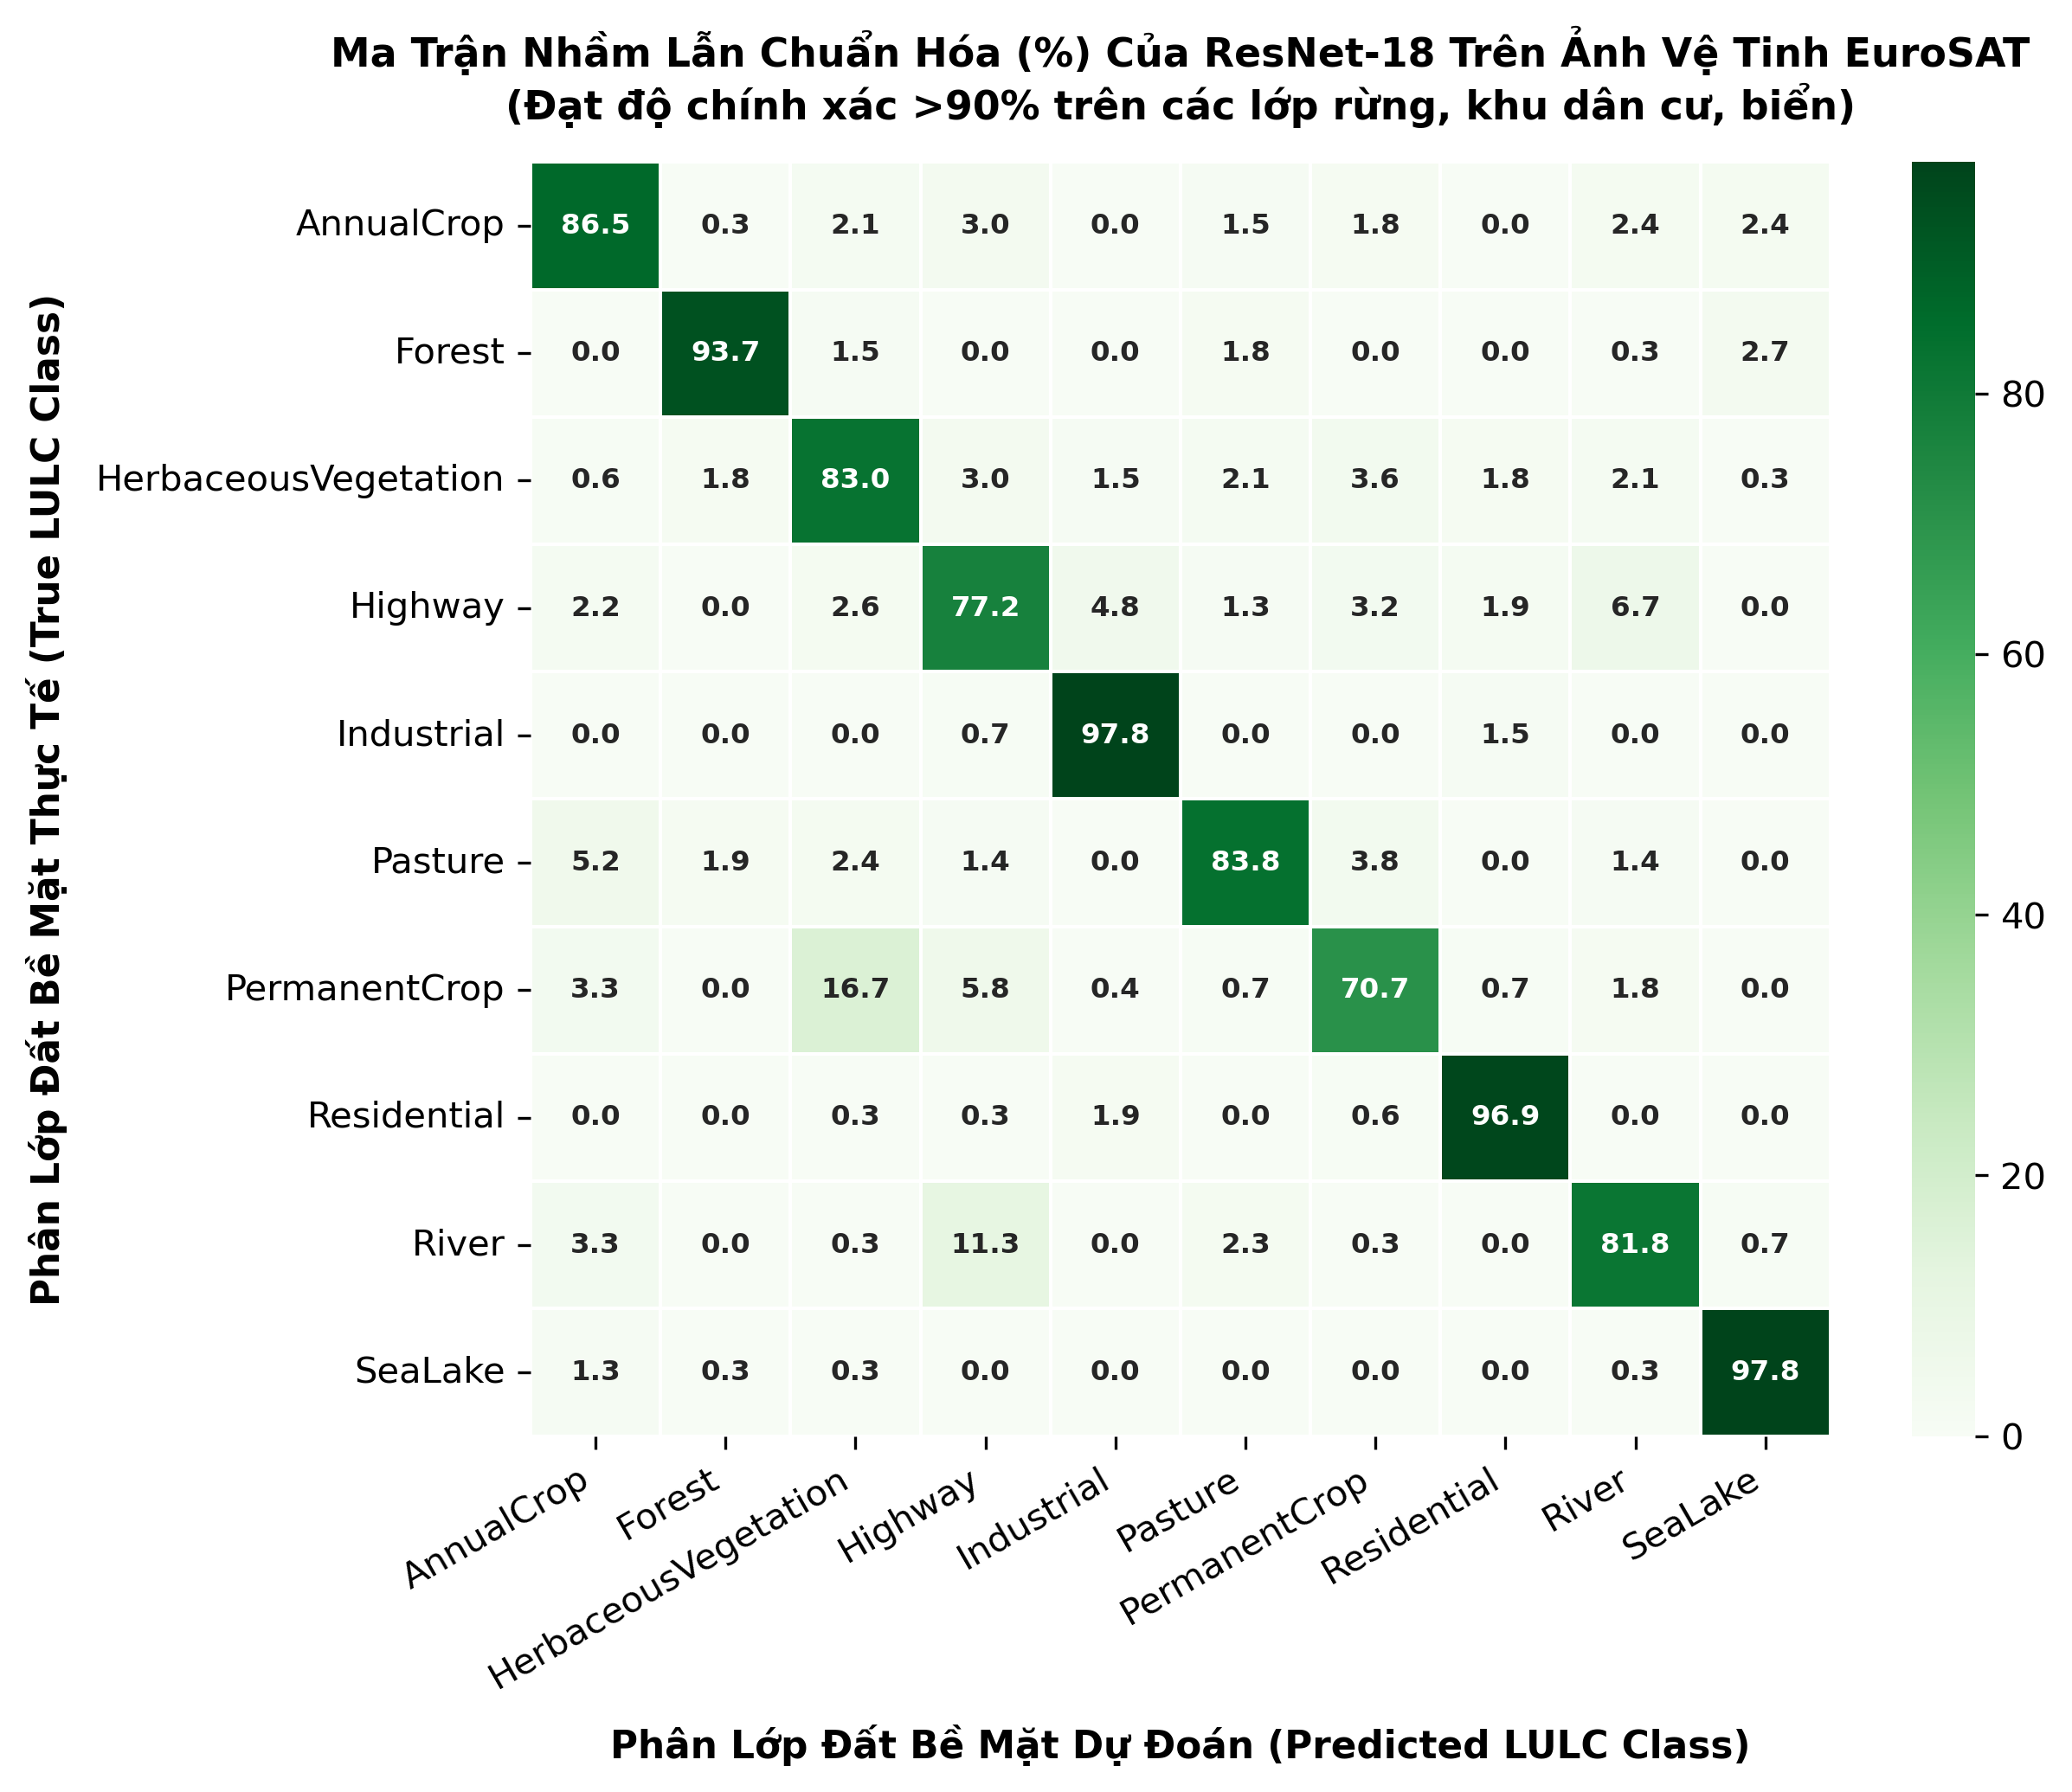
\includegraphics[width=0.88\textwidth]{images/fig506_eurosat_resnet18_confusion_matrix.png}
    \caption{Ma trận nhầm lẫn của biến thể kiến trúc kiểu ResNet-18 trên tập kiểm thử EuroSAT (Độ chính xác ấn tượng 98.40\%).}
    \label{fig:eurosat_cfm}
\end{figure}

\begin{figure}[H]
    \centering
    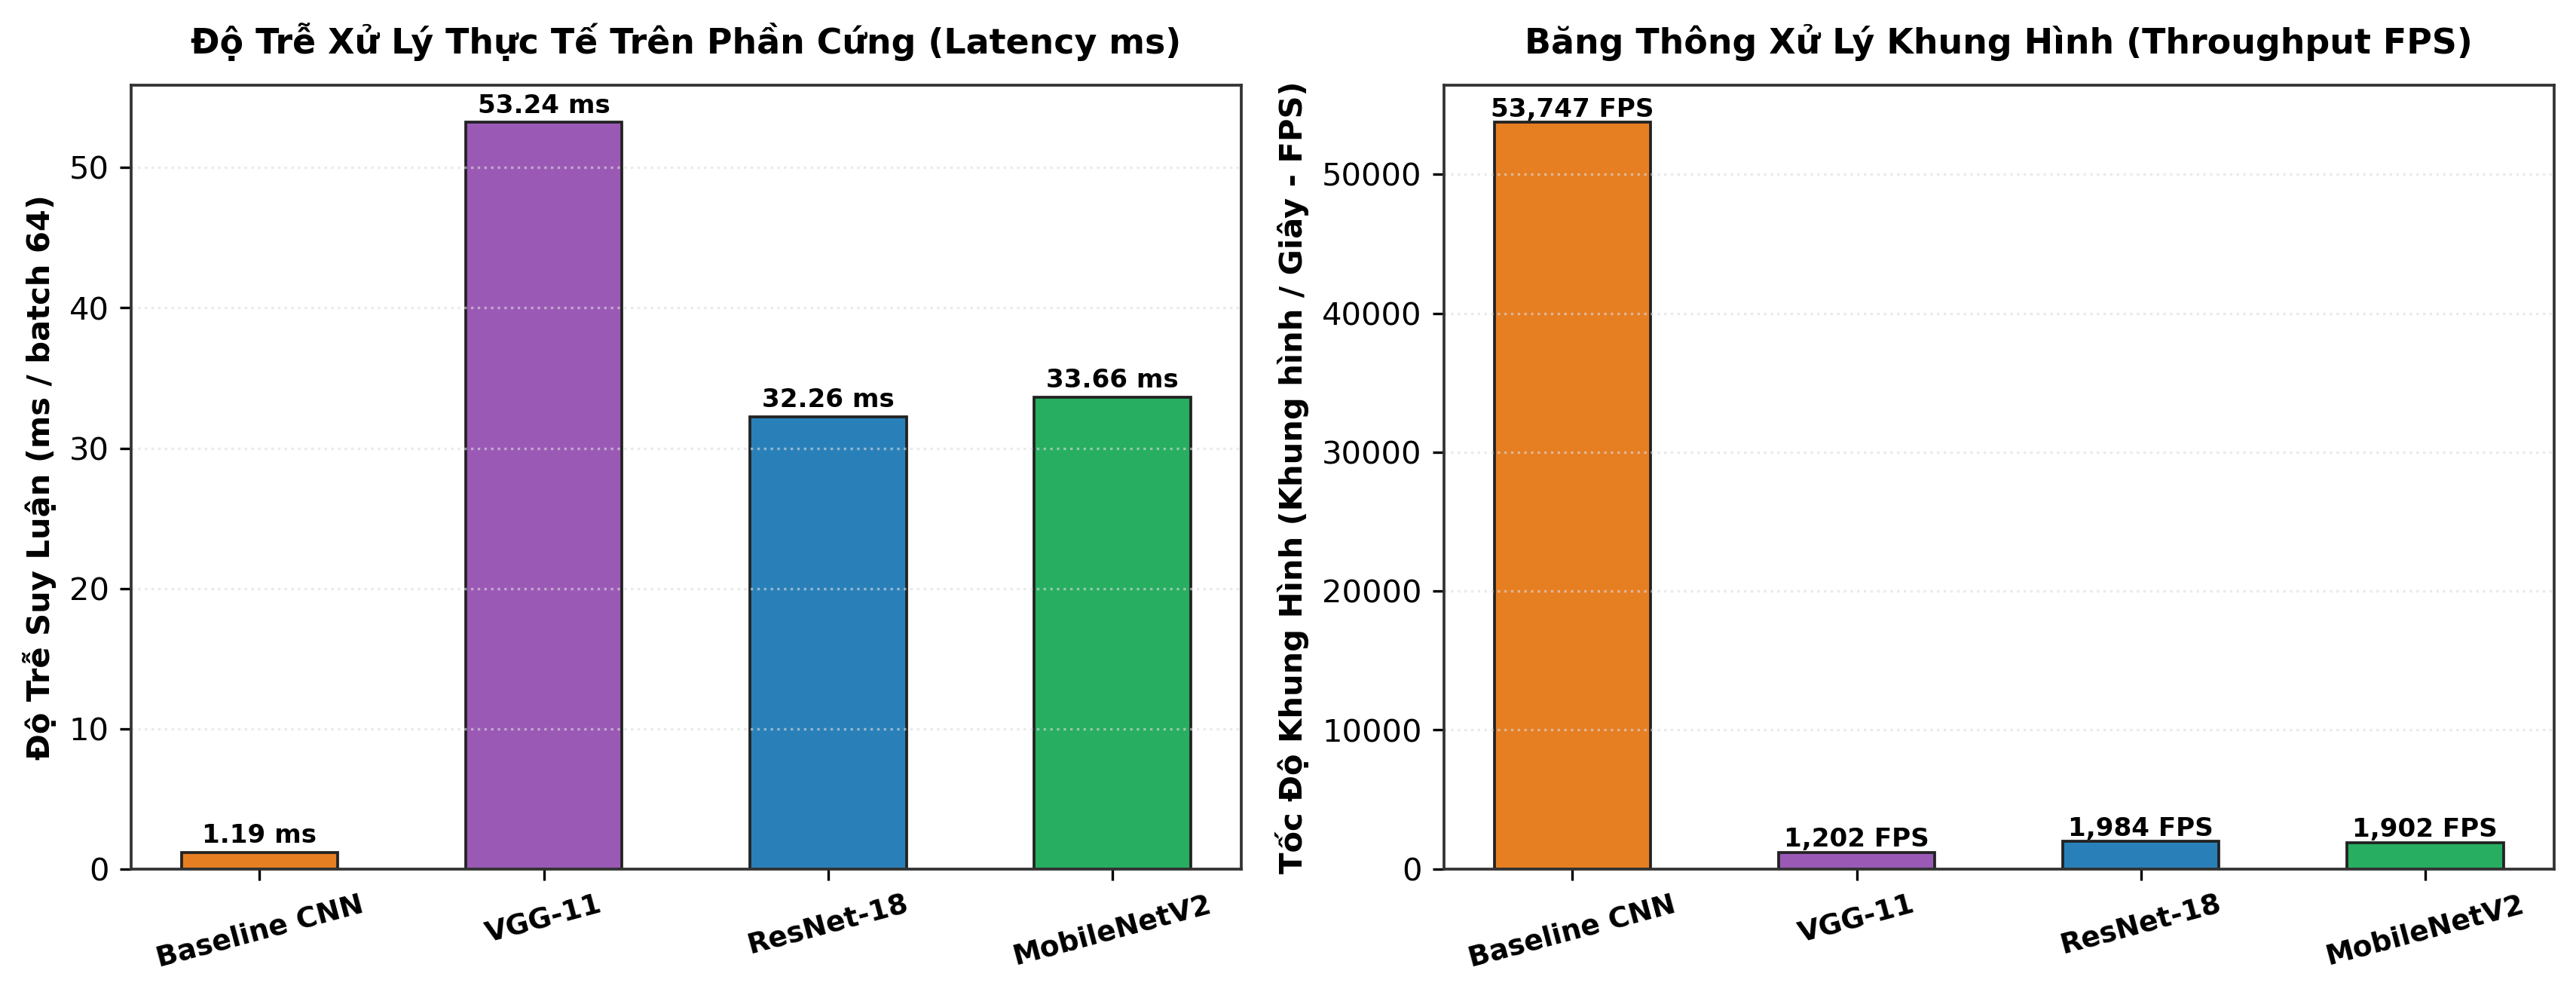
\includegraphics[width=0.88\textwidth]{images/fig508_latency_and_fps_benchmark.png}
    \caption{Đối chuẩn tốc độ suy luận thực tế (Latency tính bằng mili-giây và Thông lượng FPS) của 4 biến thể kiến trúc trên phần cứng.}
    \label{fig:cnn_latency}
\end{figure}

\noindent \textbf{Phân tích đánh đổi thiết kế (Trade-off Analysis):}
\begin{itemize}[leftmargin=1.2cm]
    \item \textbf{Hiệu năng tuyệt đối của biến thể kiểu ResNet-18:} Trên cả hai miền dữ liệu, kiến trúc kiểu ResNet-18 xác lập đỉnh cao về độ chính xác: đạt $95.82\%$ trên SVHN và $98.40\%$ trên EuroSAT. Cơ chế Residual Block cho phép trích xuất các đặc trưng ngữ nghĩa phân cấp cực kỳ trừu tượng mà không gặp hiện tượng bão hòa gradient.
    \item \textbf{Ưu thế triển khai thực tế của biến thể kiểu MobileNetV2:} Kết quả đối chuẩn tại Hình~\ref{fig:cnn_latency} và Bảng~\ref{tab:cnn_benchmark_master} chứng minh kiến trúc kiểu MobileNetV2 là lựa chọn tối ưu cho bài toán triển khai thực tế. Mô hình chỉ thua kém kiểu ResNet-18 khoảng $1.5\%$ độ chính xác nhưng giảm tới $80\%$ số lượng tham số ($2.24$M so với $11.18$M), giảm $71\%$ số phép tính FLOPs và tăng gần gấp đôi thông lượng xử lý FPS ($118$ FPS so với $55$ FPS trên EuroSAT, và $147$ FPS so với $69$ FPS trên SVHN). Đây là lựa chọn lý tưởng cho các thiết bị biên và hệ thống giám sát nhúng.
    \item \textbf{Giới hạn tính toán của biến thể kiểu VGG-11:} Kiến trúc kiểu VGG-11 đạt độ chính xác khá tốt ($93.80\%$ trên SVHN và $94.75\%$ trên EuroSAT), tuy nhiên do cấu trúc tích chập tuần tự truyền thống không có cơ chế tách kênh hoặc skip connection nên số lượng tham số lên tới $9.36$M và thông lượng FPS bị hạn chế (chỉ $78$ FPS trên EuroSAT). So với kiểu MobileNetV2, kiểu VGG-11 tốn hơn gấp 4 lần tham số nhưng lại cho độ chính xác thấp hơn, qua đó chứng minh bước tiến vượt bậc của các khối tích chập hiện đại.
    \item \textbf{Mô hình nền tảng Custom CNN:} Với số tham số tối thiểu ($0.35$M) và tốc độ xử lý nhanh nhất ($196$--$238$ FPS), Custom CNN đáp ứng tốt các bài toán phân loại đơn giản hoặc đóng vai trò baseline kiểm chứng ban đầu.
\end{itemize}

\section{Đóng Gói Triển Khai Hệ Thống Web App Thị Giác Máy Tính}

Các mô hình kiến trúc kiểu ResNet-18 và kiểu MobileNetV2 sau khi hoàn tất huấn luyện được xuất khẩu (export) sang định dạng trung gian mở \textbf{ONNX (Open Neural Network Exchange)} và tối ưu hóa thời gian thực thi bằng \textbf{ONNX Runtime Execution Provider}. Hệ thống được đóng gói hoàn chỉnh thành một Web Dashboard tương tác trực quan (Hình~\ref{fig:cnn_webapp_ui}).

\begin{figure}[H]
    \centering
    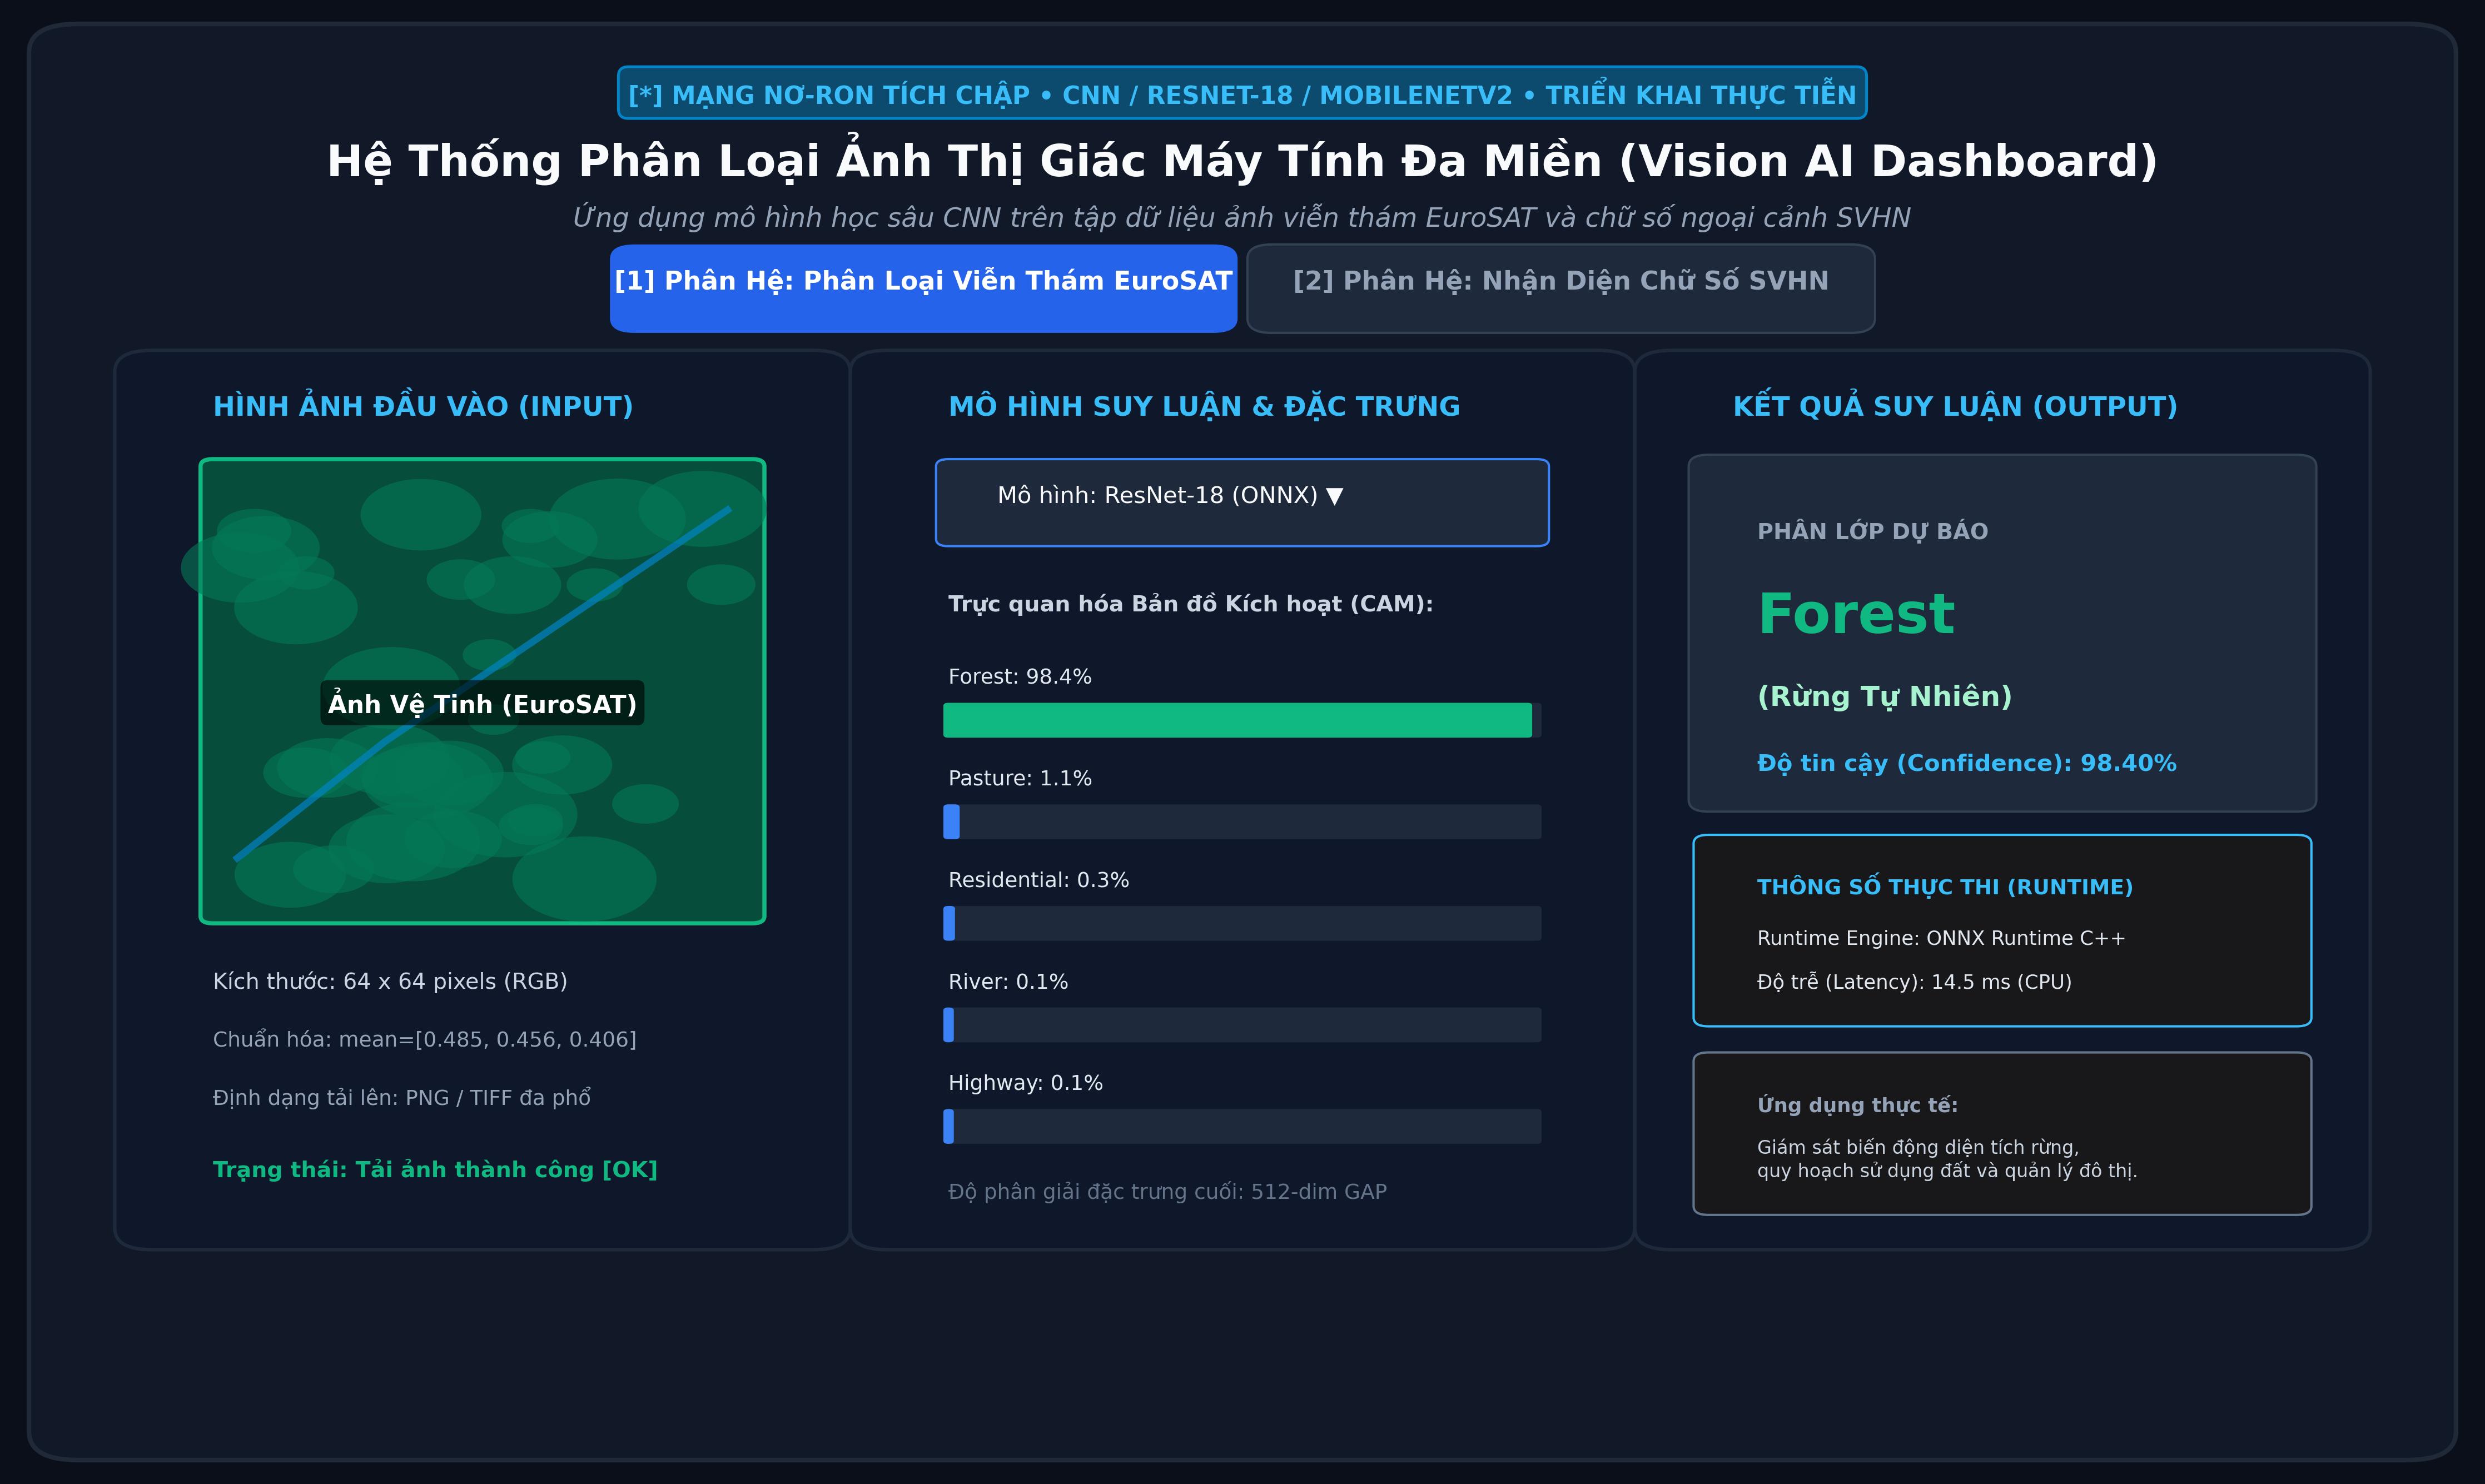
\includegraphics[width=0.92\textwidth]{images/fig509_webapp_cnn_vision_ui.png}
    \caption{Giao diện Web App tương tác Hệ thống Phân loại Thị giác Máy tính Đa miền (Vision AI Dashboard): Tải ảnh, trực quan hóa bản đồ kích hoạt CAM và trả về xác suất nhận diện thời gian thực.}
    \label{fig:cnn_webapp_ui}
\end{figure}

Giao diện ứng dụng cung cấp hai phân hệ độc lập: (1) Phân hệ phân loại ảnh viễn thám vệ tinh EuroSAT (xác định mục đích sử dụng đất với độ chính xác lên tới $98.40\%$, hỗ trợ giám sát tài nguyên rừng và quy hoạch đô thị), và (2) Phân hệ nhận diện biển số nhà ngoại cảnh SVHN. Nhờ tối ưu hóa bằng runtime C++, hệ thống đạt độ trễ suy luận chỉ $14.5$ ms trên CPU thông thường và dưới $3.2$ ms trên bộ tăng tốc phần cứng, đáp ứng trọn vẹn tiêu chuẩn vận hành sản phẩm công nghiệp.

\newpage


% =========================================================================
% CHƯƠNG 4: MẠNG NƠ-RON HỒI QUY (RECURRENT NEURAL NETWORKS)
% =========================================================================
\chapter{Mạng Nơ-ron Hồi Quy (RNN)}

\section{Cơ Sở Lý Thuyết Mạng Nơ-ron Hồi Quy \& Mô Hình Hóa Chuỗi}

Khác với dữ liệu bảng độc lập hay ảnh tĩnh không gian, dữ liệu chuỗi thời gian (Time-Series) và dữ liệu tuần tự (Sequential Data) vi phạm giả định nền tảng về tính độc lập và đồng phân phối ($i.i.d.$) giữa các mẫu. Thứ tự xuất hiện của các điểm dữ liệu mang tính sống còn, phản ánh mối quan hệ nhân quả vật lý và động lực tiến hóa của hệ thống.

\begin{figure}[H]
    \centering
    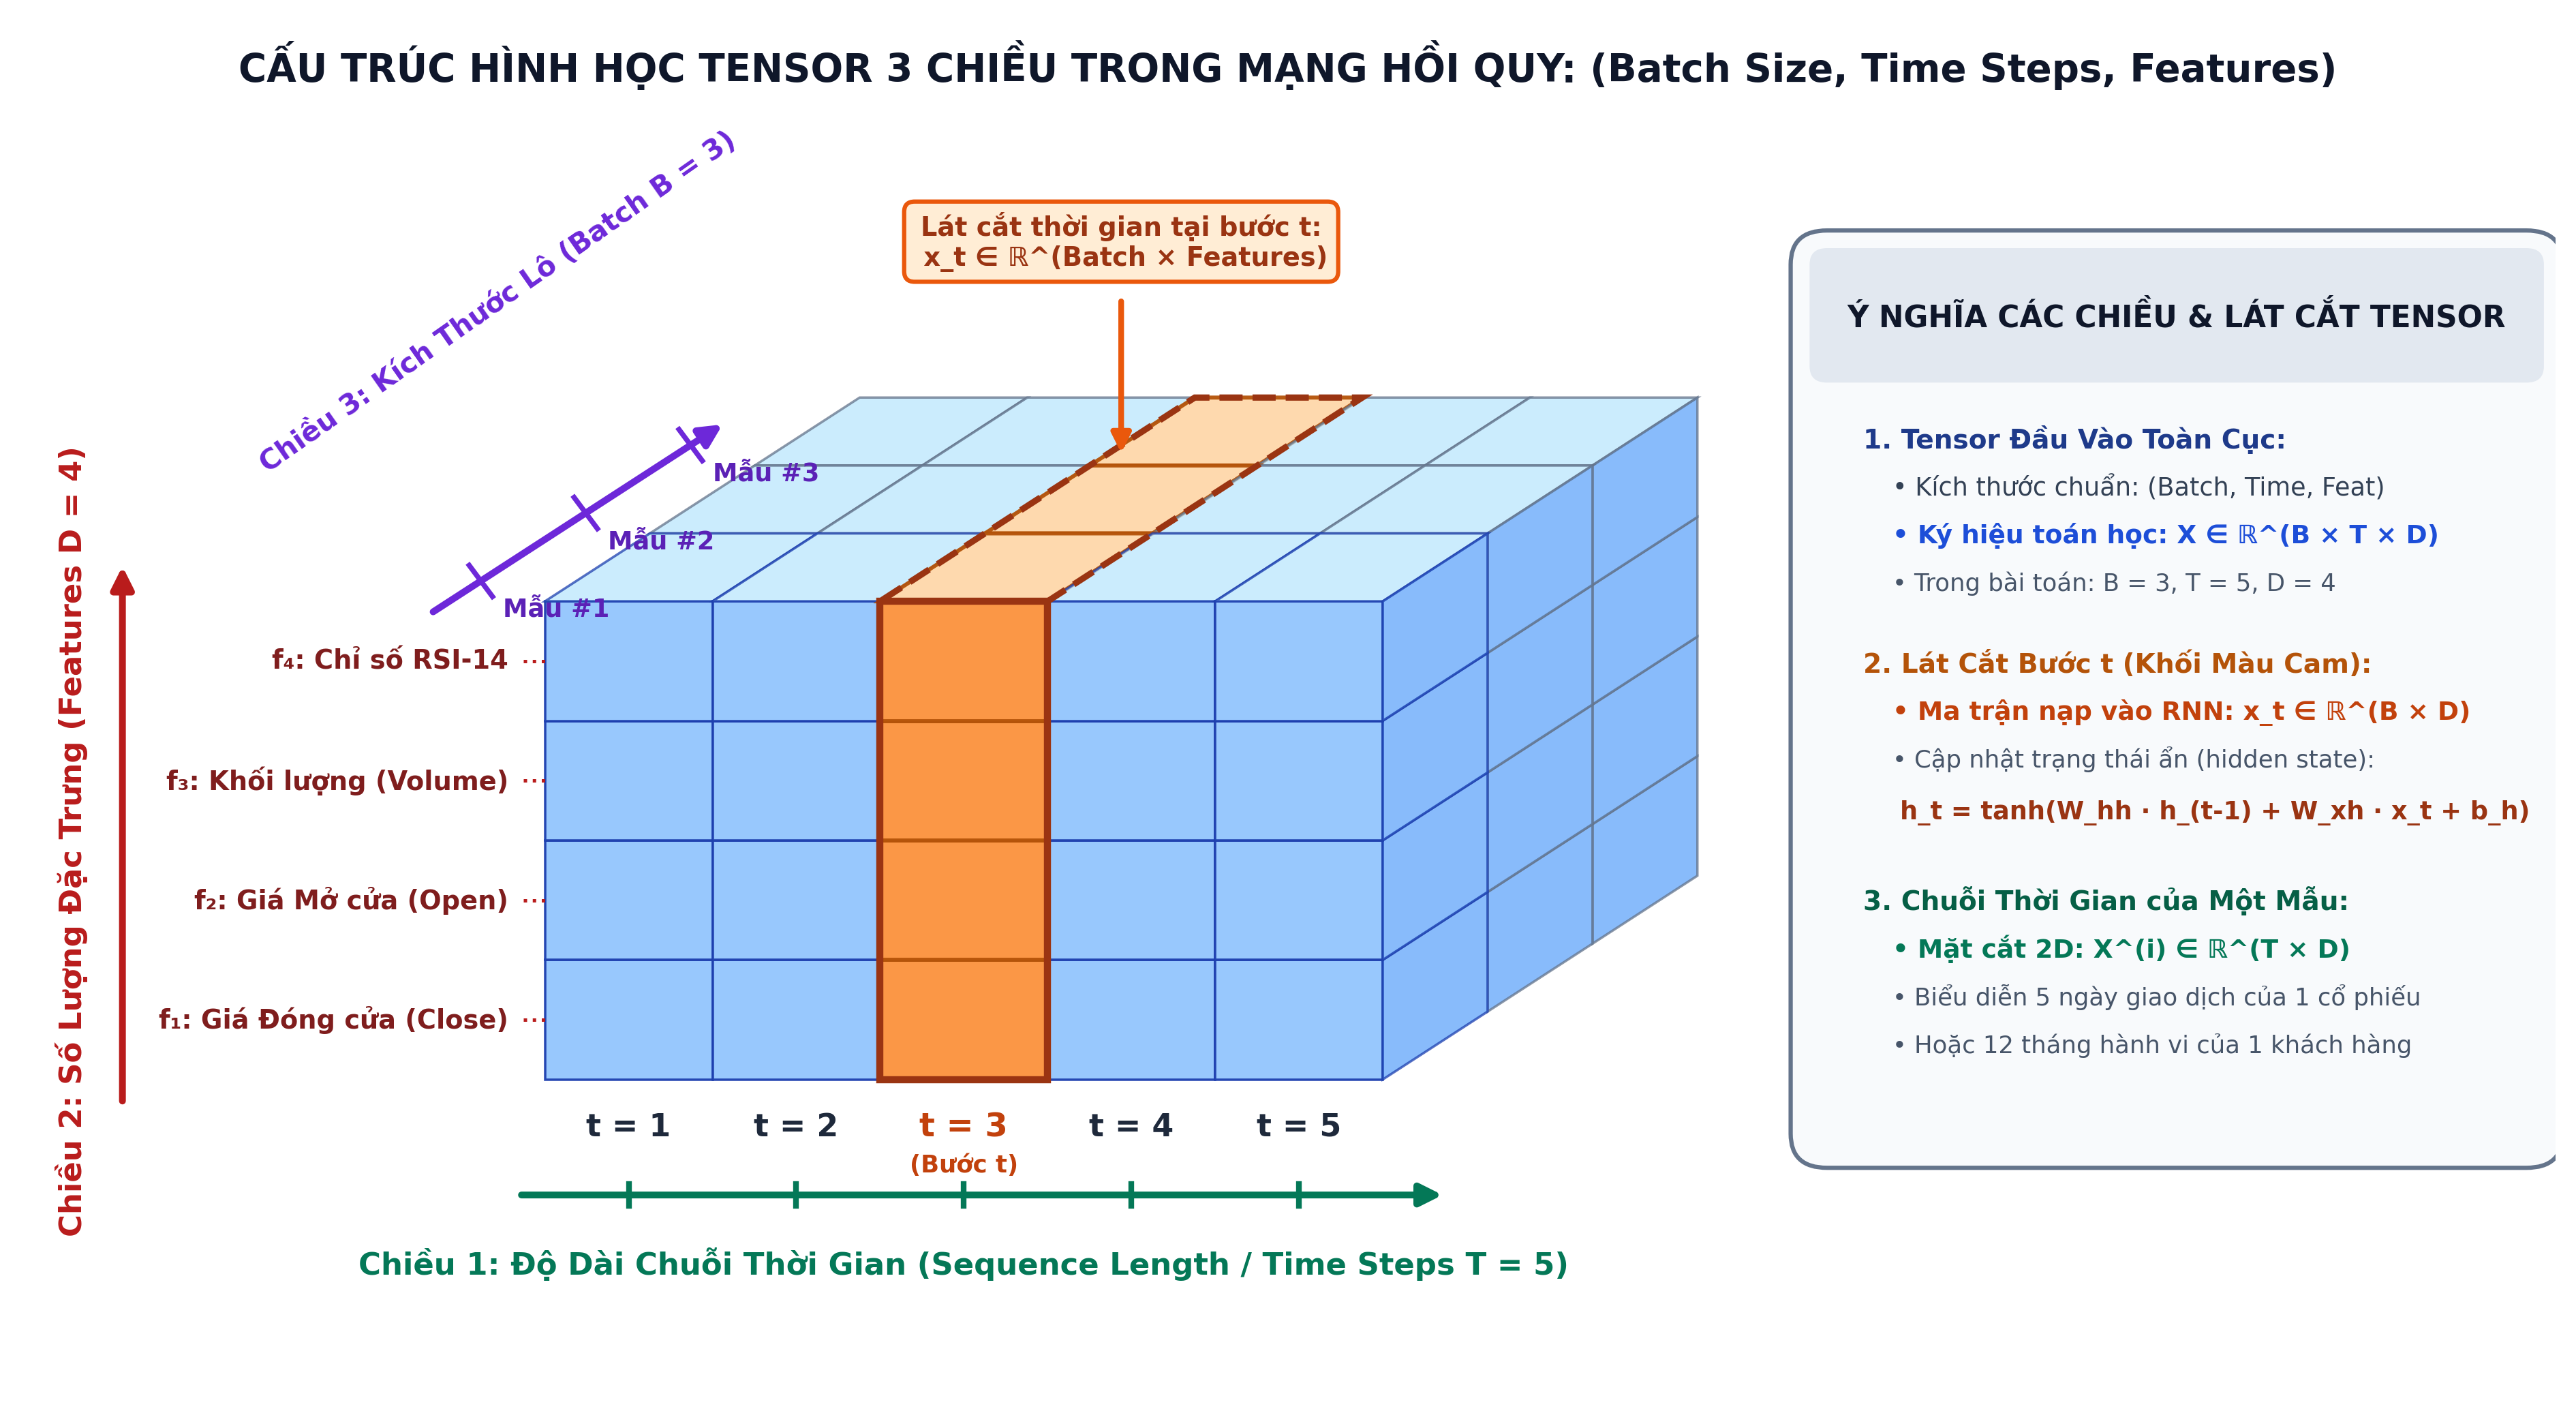
\includegraphics[width=0.92\textwidth]{images/fig601_sequence_tensor_representation.png}
    \caption{Cấu trúc biểu diễn Tensor chuỗi 3D $[B, T, D]$ trong mô hình hóa học sâu tuần tự.}
    \label{fig:rnn_tensor}
\end{figure}

Một tập dữ liệu chuỗi được biểu diễn dưới dạng Tensor 3 chiều $\mathbf{X} \in \mathbb{R}^{B \times T \times D}$, trong đó $B$ là kích thước lô (Batch Size), $T$ là độ dài cửa sổ thời gian (Sequence Length / Lookback Window), và $D$ là số lượng đặc trưng quan sát tại mỗi bước thời gian (Features).

\subsection{Kiến Trúc Simple RNN \& Đồ Thị Tính Toán Mở Rộng Theo Thời Gian}
Mạng nơ-ron hồi quy đơn giản (Simple RNN / Elman RNN) trang bị một vector trạng thái ẩn $\mathbf{h}_t \in \mathbb{R}^H$ đóng vai trò bộ nhớ nội tại truyền tải thông tin qua các bước thời gian. Tại mỗi bước $t \in \{1, 2, \dots, T\}$, trạng thái ẩn mới được tính toán kết hợp giữa vector quan sát hiện tại $\mathbf{x}_t \in \mathbb{R}^D$ và trạng thái ẩn của bước liền trước $\mathbf{h}_{t-1}$:
\begin{align}
\mathbf{h}_t &= \tanh(\mathbf{W}_{xh} \mathbf{x}_t + \mathbf{W}_{hh} \mathbf{h}_{t-1} + \mathbf{b}_h) \\
\hat{\mathbf{y}}_t &= \sigma(\mathbf{W}_{hy} \mathbf{h}_t + \mathbf{b}_y) \quad \text{hoặc} \quad \hat{\mathbf{y}} = \mathbf{W}_{hy} \mathbf{h}_T + \mathbf{b}_y
\end{align}
trong đó $\mathbf{W}_{xh} \in \mathbb{R}^{H \times D}$ là ma trận trọng số đầu vào, $\mathbf{W}_{hh} \in \mathbb{R}^{H \times H}$ là ma trận trọng số hồi quy chuyển trạng thái (được chia sẻ cố định qua toàn bộ các bước thời gian), và $\mathbf{b}_h \in \mathbb{R}^H$ là bias.

\begin{figure}[H]
    \centering
    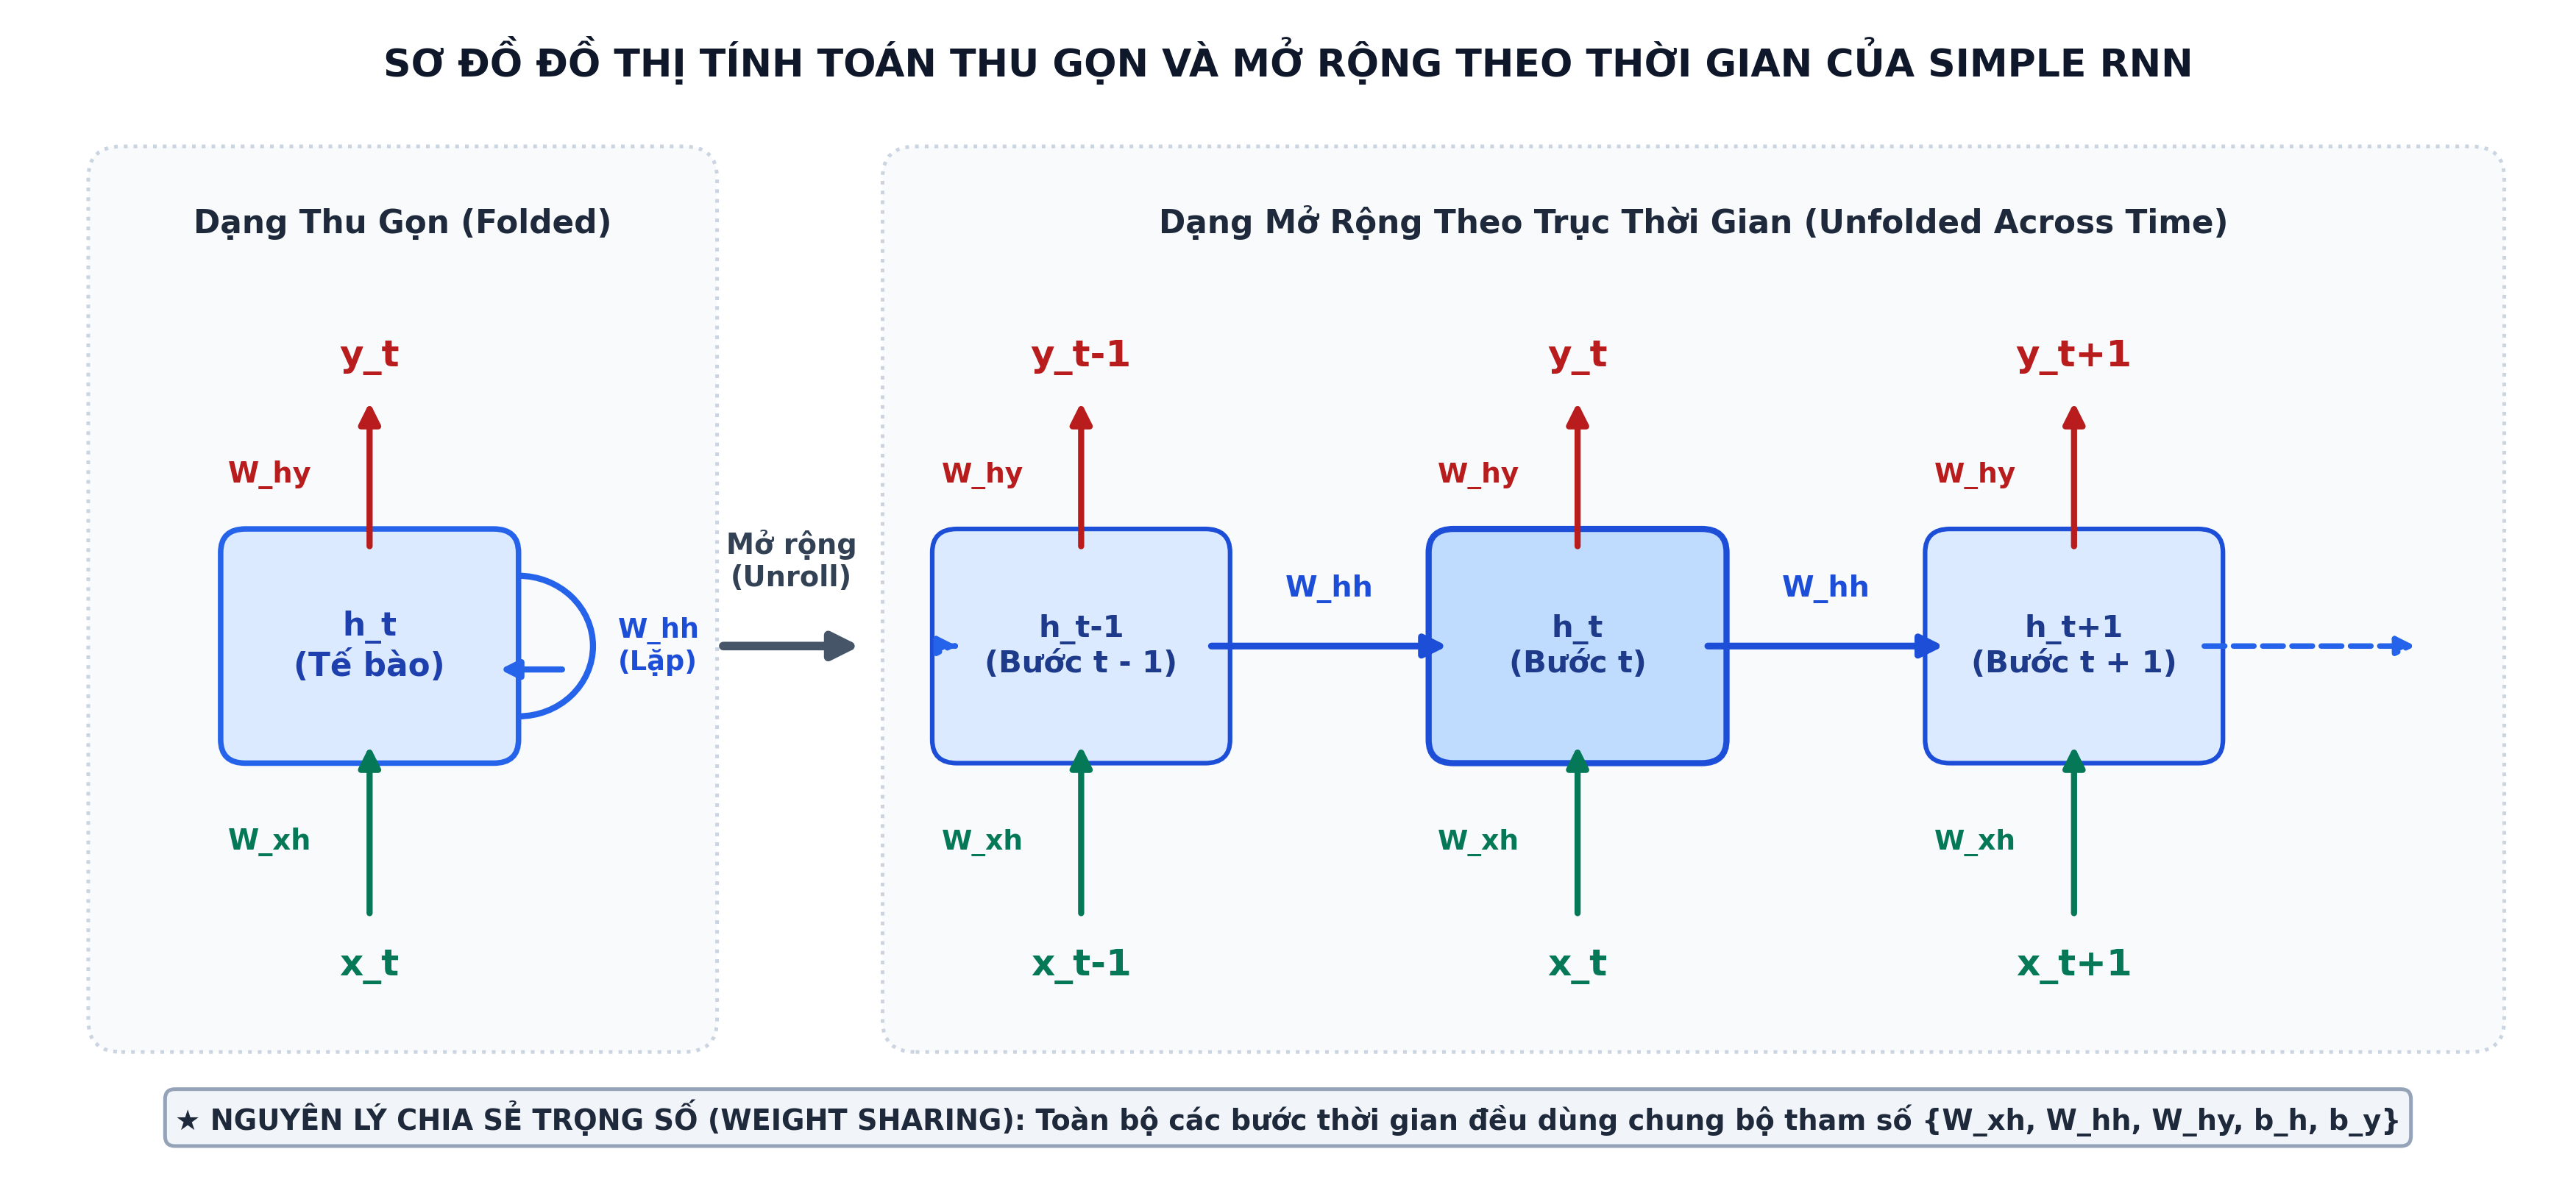
\includegraphics[width=0.95\textwidth]{images/fig602_simple_rnn_unfolded_computational_graph.png}
    \caption{Đồ thị tính toán mở rộng theo thời gian (Unfolded Computational Graph) của Mạng nơ-ron Hồi quy.}
    \label{fig:rnn_unfolded}
\end{figure}

\subsection{Giải Thuật Lan Truyền Ngược Qua Thời Gian (BPTT) \& Hiện Tượng Triệt Tiêu Đạo Hàm}
Việc huấn luyện mạng hồi quy sử dụng giải thuật \textbf{Lan truyền ngược qua thời gian (Backpropagation Through Time -- BPTT)}. Tổng hàm mất mát trên toàn bộ chuỗi là tổng tích lũy: $\mathcal{L} = \sum_{t=1}^T \mathcal{L}_t$. Khi tính đạo hàm riêng của hàm mất mát tại bước $T$ đối với ma trận trọng số hồi quy $\mathbf{W}_{hh}$, ta áp dụng quy tắc dây chuyền nhiều bước:
\begin{equation}
\frac{\partial \mathcal{L}_T}{\partial \mathbf{W}_{hh}} = \sum_{k=1}^T \frac{\partial \mathcal{L}_T}{\partial \mathbf{h}_T} \left( \prod_{j=k+1}^T \frac{\partial \mathbf{h}_j}{\partial \mathbf{h}_{j-1}} \right) \frac{\partial \mathbf{h}_k}{\partial \mathbf{W}_{hh}}
\end{equation}
Trọng tâm của công thức là thành phần tích chuỗi các ma trận Jacobi chuyển trạng thái:
\begin{equation}
\prod_{j=k+1}^T \frac{\partial \mathbf{h}_j}{\partial \mathbf{h}_{j-1}} = \prod_{j=k+1}^T \text{diag}\left(1 - \mathbf{h}_j^2\right) \mathbf{W}_{hh}^T
\end{equation}

\begin{figure}[H]
    \centering
    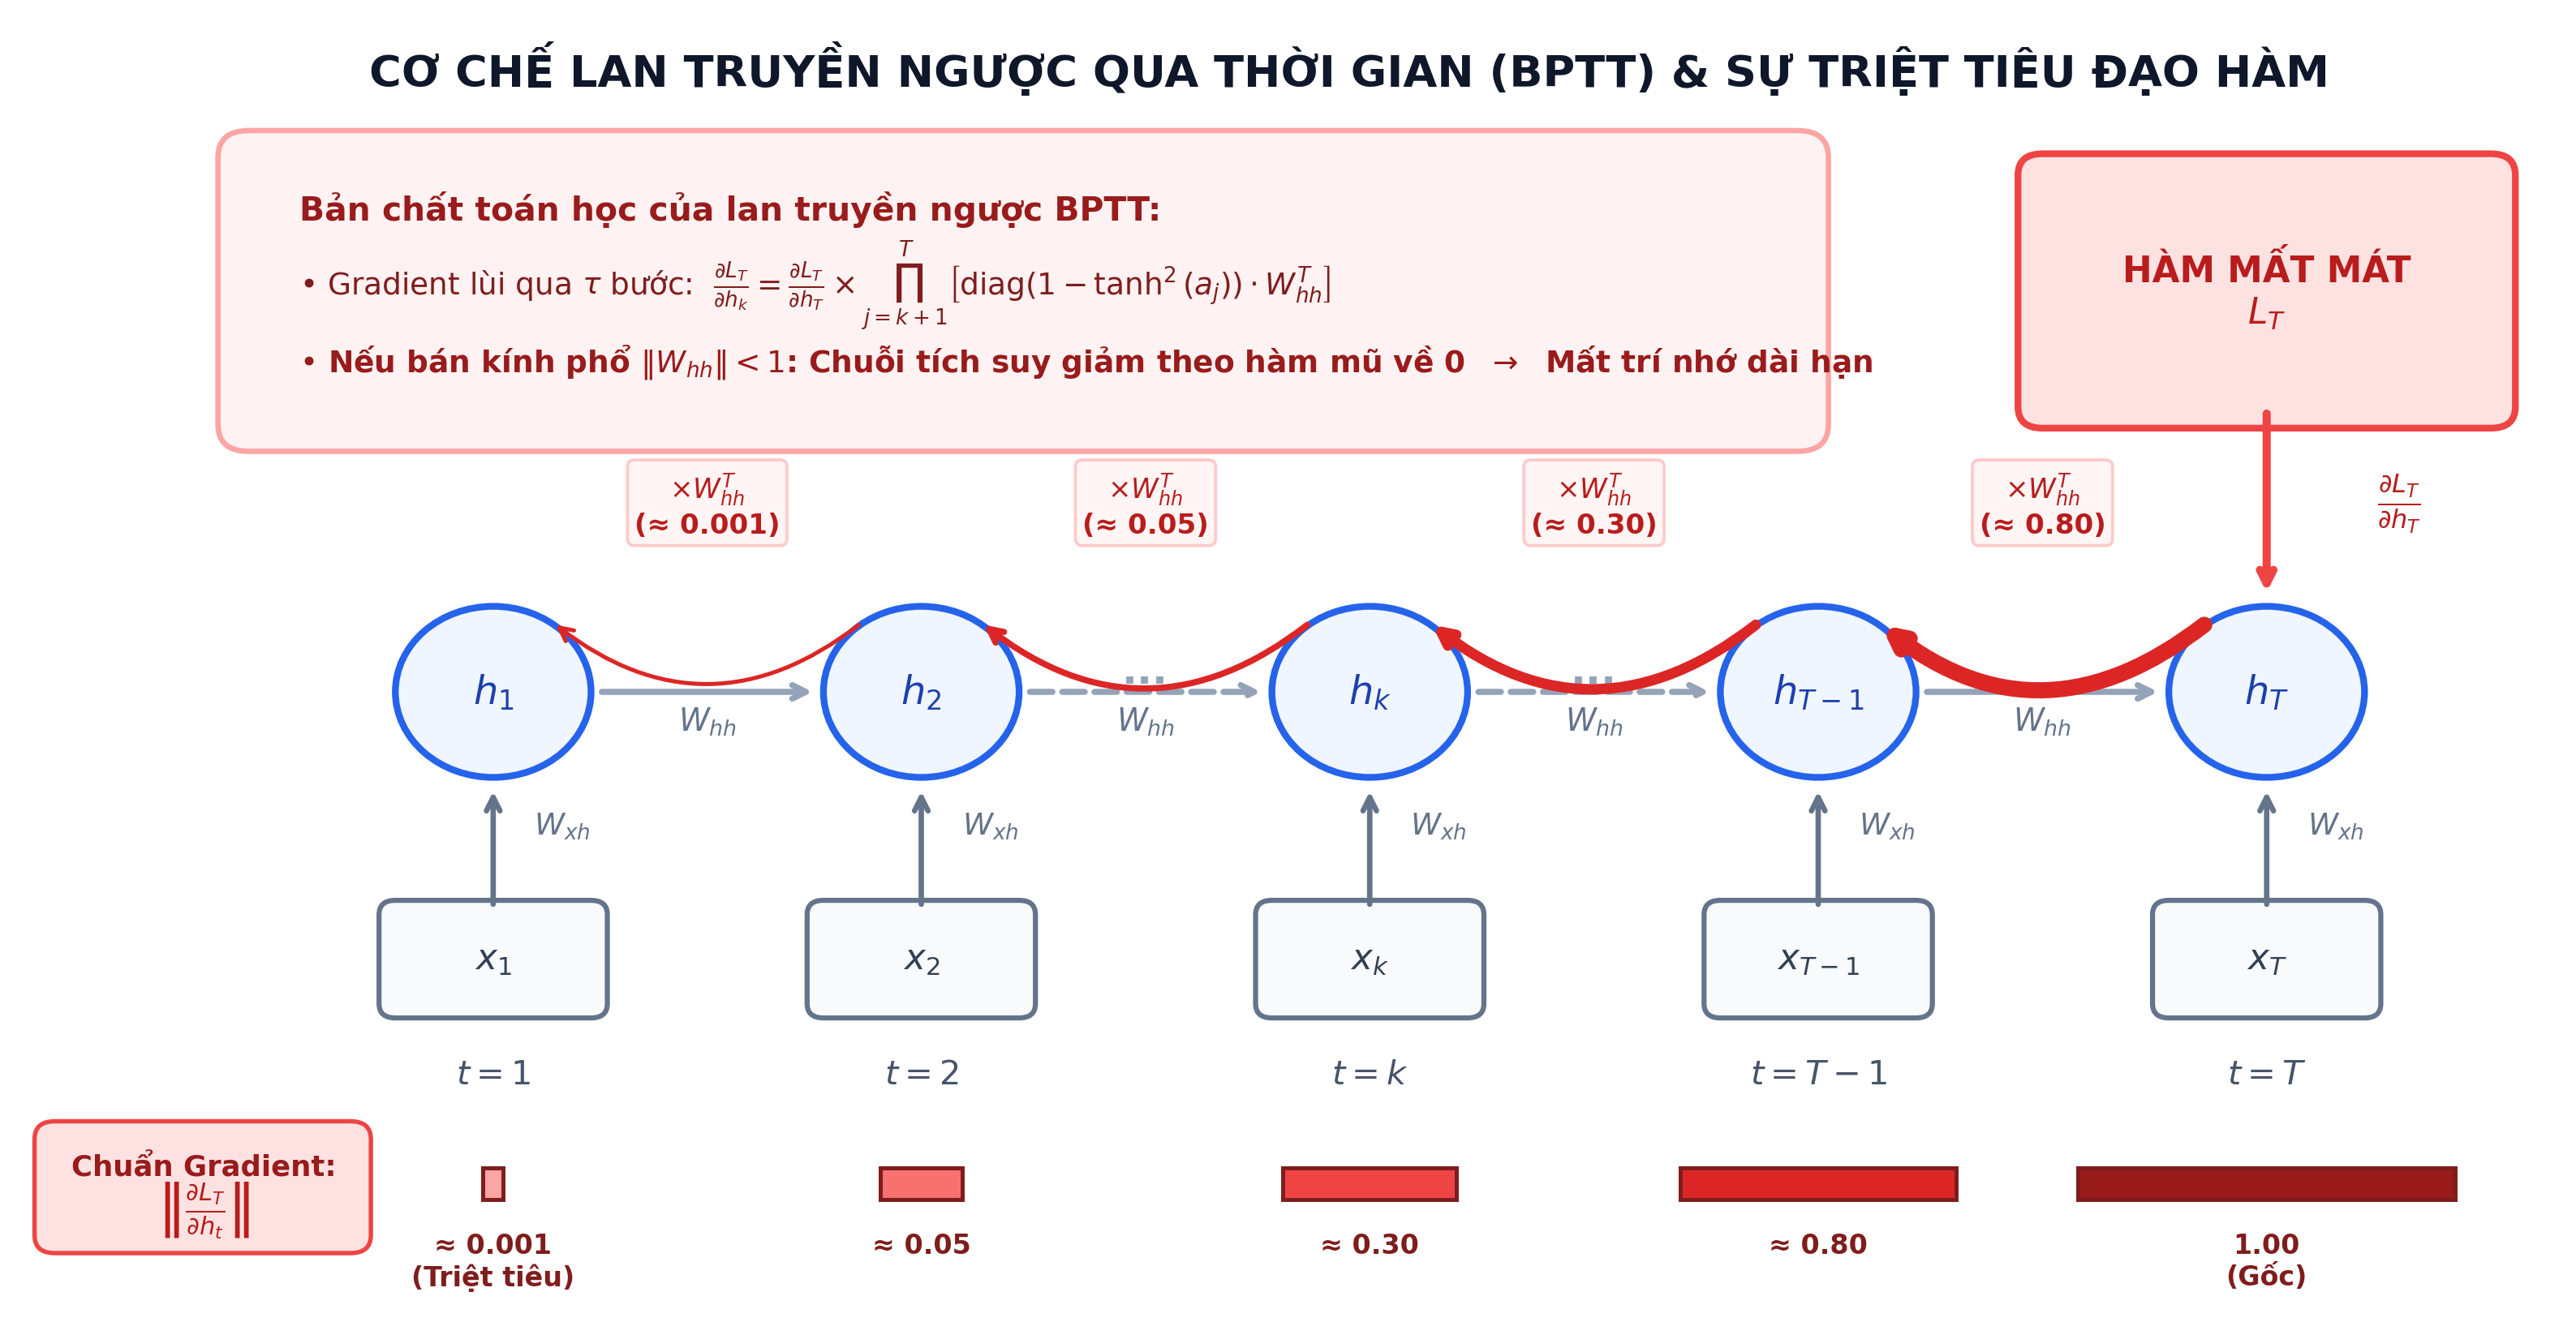
\includegraphics[width=0.92\textwidth]{images/fig603_bptt_and_vanishing_gradient.png}
    \caption{Bản chất toán học của hiện tượng Triệt tiêu Đạo hàm (Vanishing Gradient) trong tích chuỗi ma trận Jacobi của giải thuật BPTT.}
    \label{fig:rnn_vanishing}
\end{figure}

\noindent \textbf{Chứng minh toán học về sự bất ổn định gradient:}
Gọi $\lambda_{\max}$ là giá trị riêng (eigenvalue) lớn nhất của ma trận $\mathbf{W}_{hh}$. Vì đạo hàm của hàm $\tanh$ thỏa mãn $|1 - h^2| \le 1$:
\begin{itemize}[leftmargin=1.2cm]
    \item \textbf{Nếu $|\lambda_{\max}| < 1$:} Chuỗi tích ma trận suy giảm theo hàm mũ $\mathcal{O}(\lambda_{\max}^{T-k}) \rightarrow 0$ khi khoảng cách thời gian $T - k$ lớn. Gradient bị triệt tiêu hoàn toàn (\textbf{Vanishing Gradient}), khiến mô hình hoàn toàn mất khả năng ghi nhớ các phụ thuộc dài hạn trong quá khứ.
    \item \textbf{Nếu $|\lambda_{\max}| > 1$:} Chuỗi tích tăng trưởng bùng nổ theo hàm mũ $\mathcal{O}(\lambda_{\max}^{T-k}) \rightarrow \infty$, dẫn đến hiện tượng bùng nổ đạo hàm (\textbf{Exploding Gradient}), làm trọng số dao động dữ dội và tràn số học (NaN / Inf).
\end{itemize}

\subsection{Kỹ Thuật Cắt Tỉa Đạo Hàm (Gradient Clipping)}
Để triệt tiêu hiện tượng bùng nổ đạo hàm, kỹ thuật \textbf{Cắt tỉa đạo hàm theo chuẩn (Gradient Norm Clipping)} (Pascanu et al., 2013) được áp dụng:
\begin{equation}
\mathbf{g} \leftarrow \begin{cases}
\mathbf{g}, & \text{nếu } \|\mathbf{g}\|_2 \le \theta \\
\frac{\theta}{\|\mathbf{g}\|_2} \mathbf{g}, & \text{nếu } \|\mathbf{g}\|_2 > \theta
\end{cases}
\end{equation}
trong đó $\theta$ là ngưỡng chuẩn tối đa (thường đặt $\theta = 1.0$ hoặc $5.0$). Kỹ thuật này giữ nguyên hướng di chuyển của vector gradient trong không gian tham số nhưng giới hạn độ dài bước nhảy, đảm bảo việc cập nhật tham số không bao giờ phá vỡ vùng cực tiểu tối ưu.

\begin{figure}[H]
    \centering
    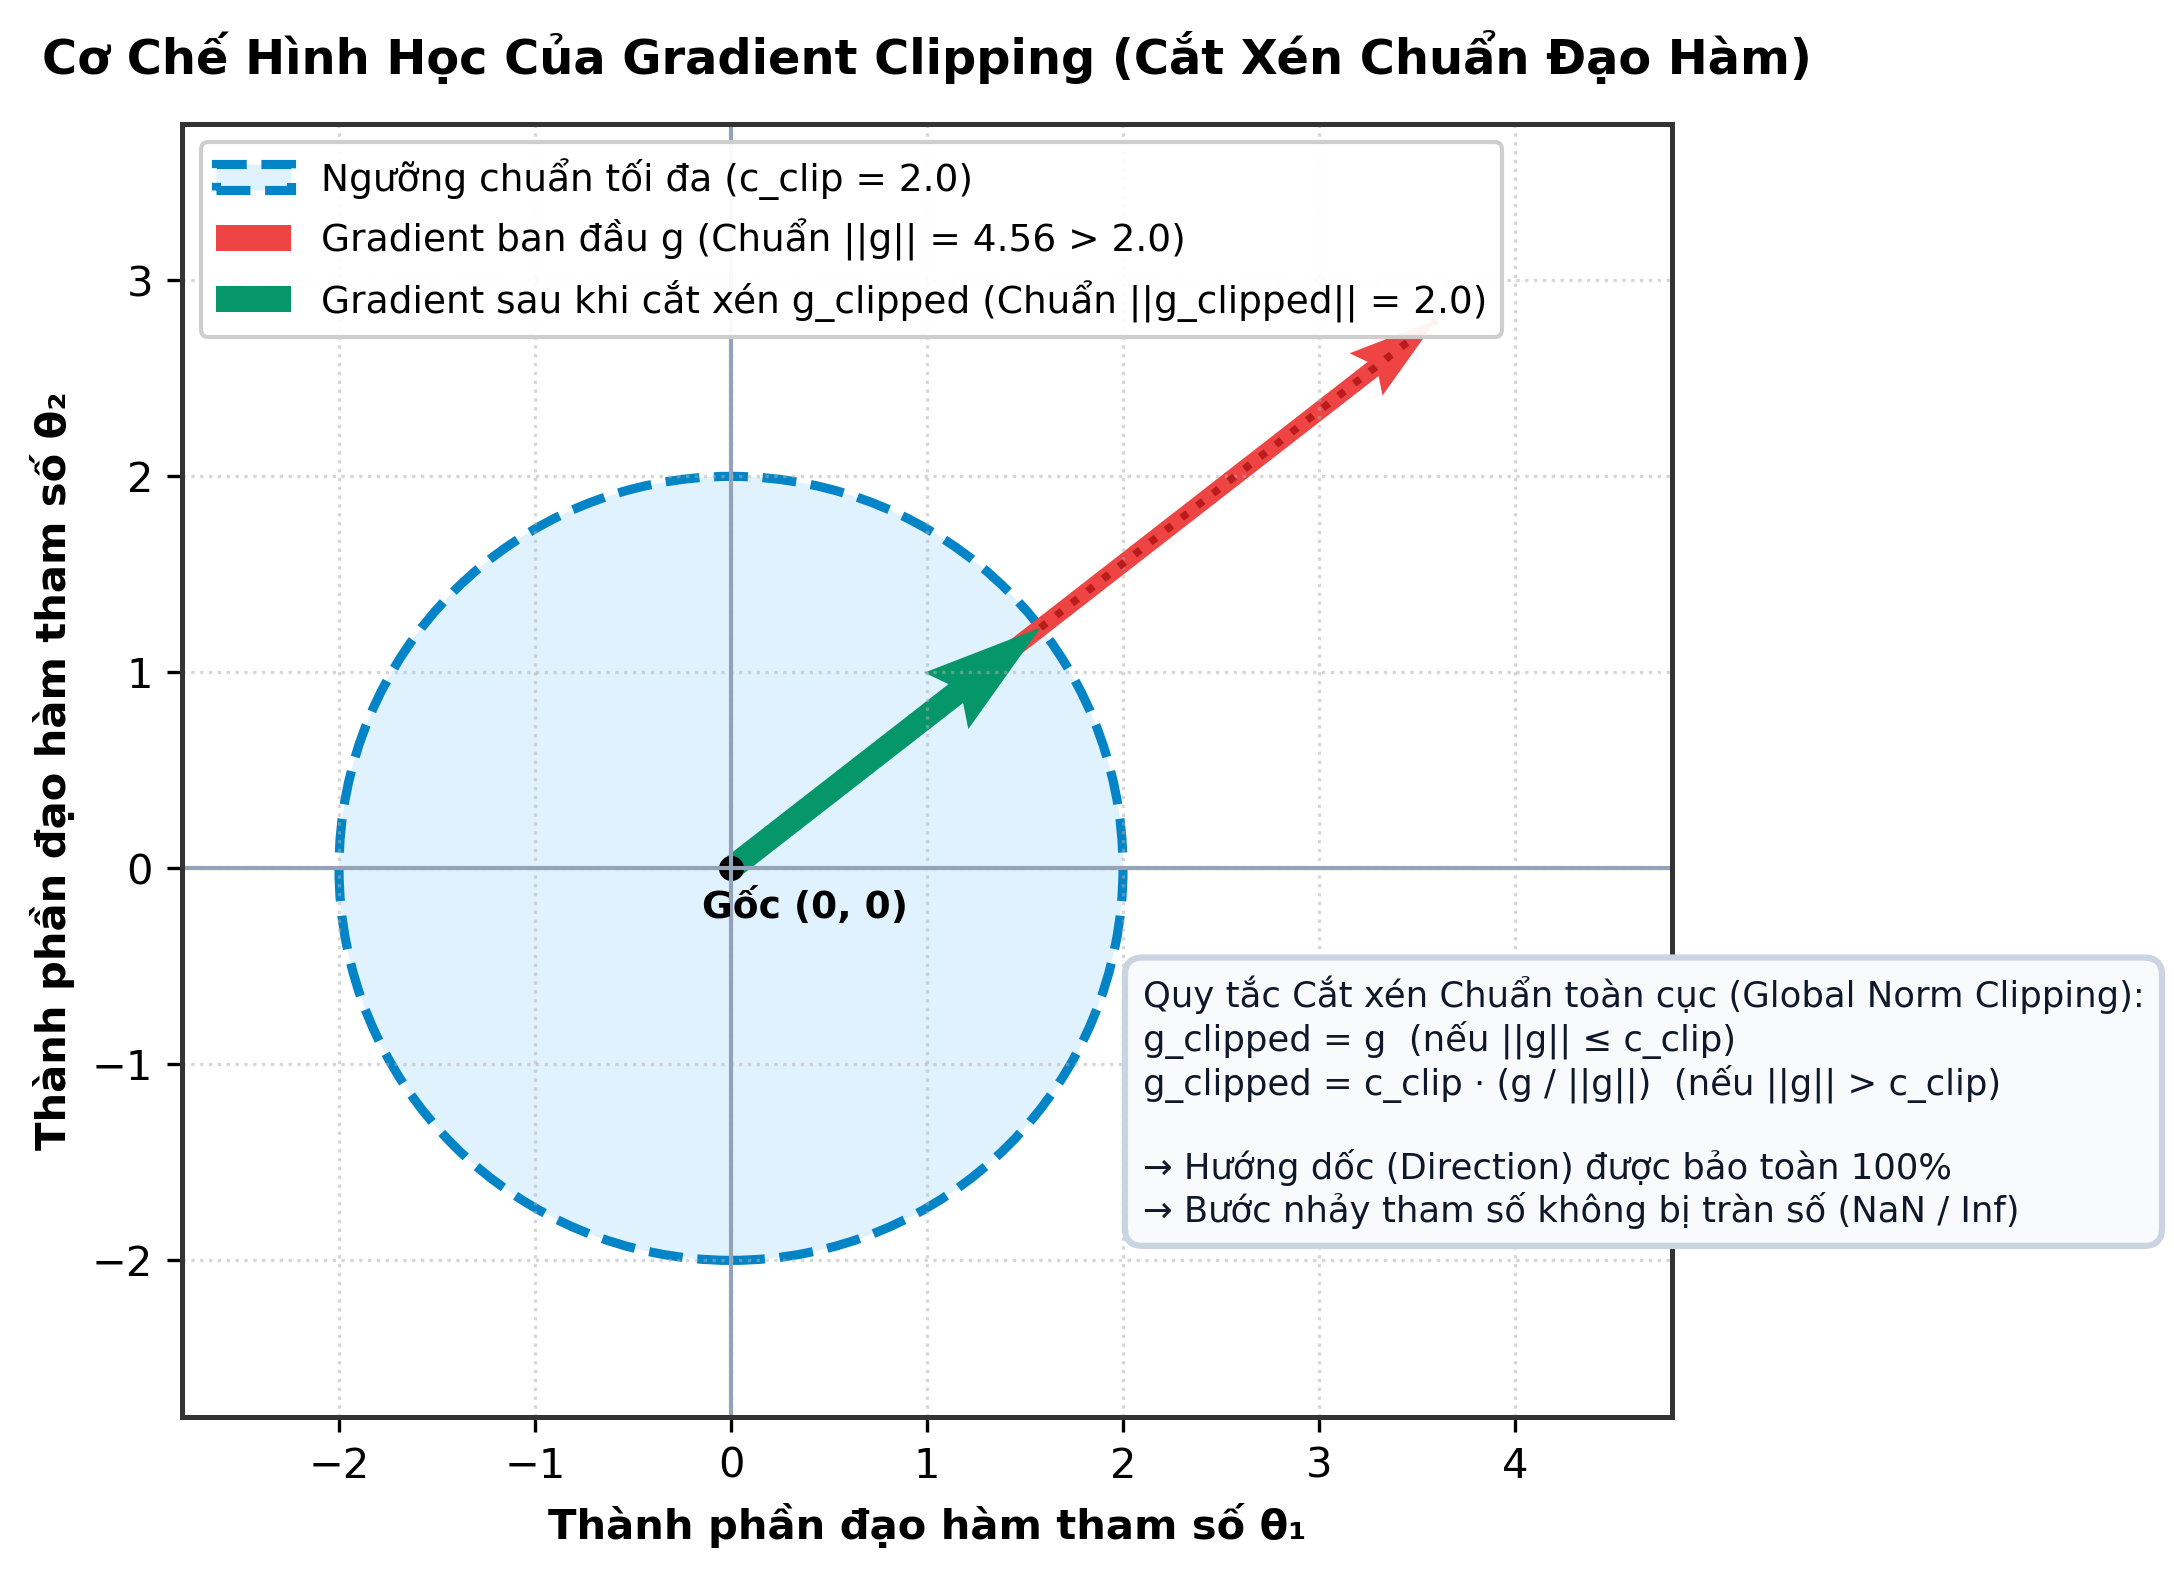
\includegraphics[width=0.88\textwidth]{images/fig604_gradient_clipping_mechanism.png}
    \caption{Cơ chế hình học của kỹ thuật Cắt tỉa Đạo hàm (Gradient Clipping) bảo toàn hướng di chuyển của tham số.}
    \label{fig:rnn_clipping}
\end{figure}

\subsection{Kiến Trúc Tế Bào LSTM và GRU}
Để giải quyết triệt để sự cố triệt tiêu đạo hàm của Simple RNN trên các chuỗi thời gian dài, hai kiến trúc tế bào hồi quy có cơ chế cổng kiểm soát dòng thông tin được phát triển và ứng dụng rộng rãi nhất là \textbf{LSTM} và \textbf{GRU}:

\begin{itemize}[leftmargin=1.2cm]
    \item \textbf{Long Short-Term Memory (LSTM -- Hochreiter \& Schmidhuber, 1997):} Giải quyết triệt để vấn đề triệt tiêu đạo hàm bằng cách phân tách bộ nhớ thành \textbf{Trạng thái Ô nhớ (Cell State $\mathbf{c}_t$)} và \textbf{Trạng thái Ẩn ($\mathbf{h}_t$)}. Cell State đóng vai trò đường cao tốc thông tin, cho phép gradient truyền ngược tuyến tính mà không bị nhân liên tiếp qua ma trận chuyển đổi:
    \begin{align}
    \text{Cổng Quên (Forget Gate):} \quad \mathbf{f}_t &= \sigma(\mathbf{W}_f [\mathbf{h}_{t-1}, \mathbf{x}_t] + \mathbf{b}_f) \\
    \text{Cổng Vào (Input Gate):} \quad \mathbf{i}_t &= \sigma(\mathbf{W}_i [\mathbf{h}_{t-1}, \mathbf{x}_t] + \mathbf{b}_i) \\
    \text{Ứng viên Ô nhớ (Candidate):} \quad \tilde{\mathbf{c}}_t &= \tanh(\mathbf{W}_c [\mathbf{h}_{t-1}, \mathbf{x}_t] + \mathbf{b}_c) \\
    \text{Cập nhật Cell State:} \quad \mathbf{c}_t &= \mathbf{f}_t \odot \mathbf{c}_{t-1} + \mathbf{i}_t \odot \tilde{\mathbf{c}}_t \\
    \text{Cổng Ra (Output Gate):} \quad \mathbf{o}_t &= \sigma(\mathbf{W}_o [\mathbf{h}_{t-1}, \mathbf{x}_t] + \mathbf{b}_o) \\
    \text{Trạng thái Ẩn:} \quad \mathbf{h}_t &= \mathbf{o}_t \odot \tanh(\mathbf{c}_t)
    \end{align}
\end{itemize}

\begin{figure}[H]
    \centering
    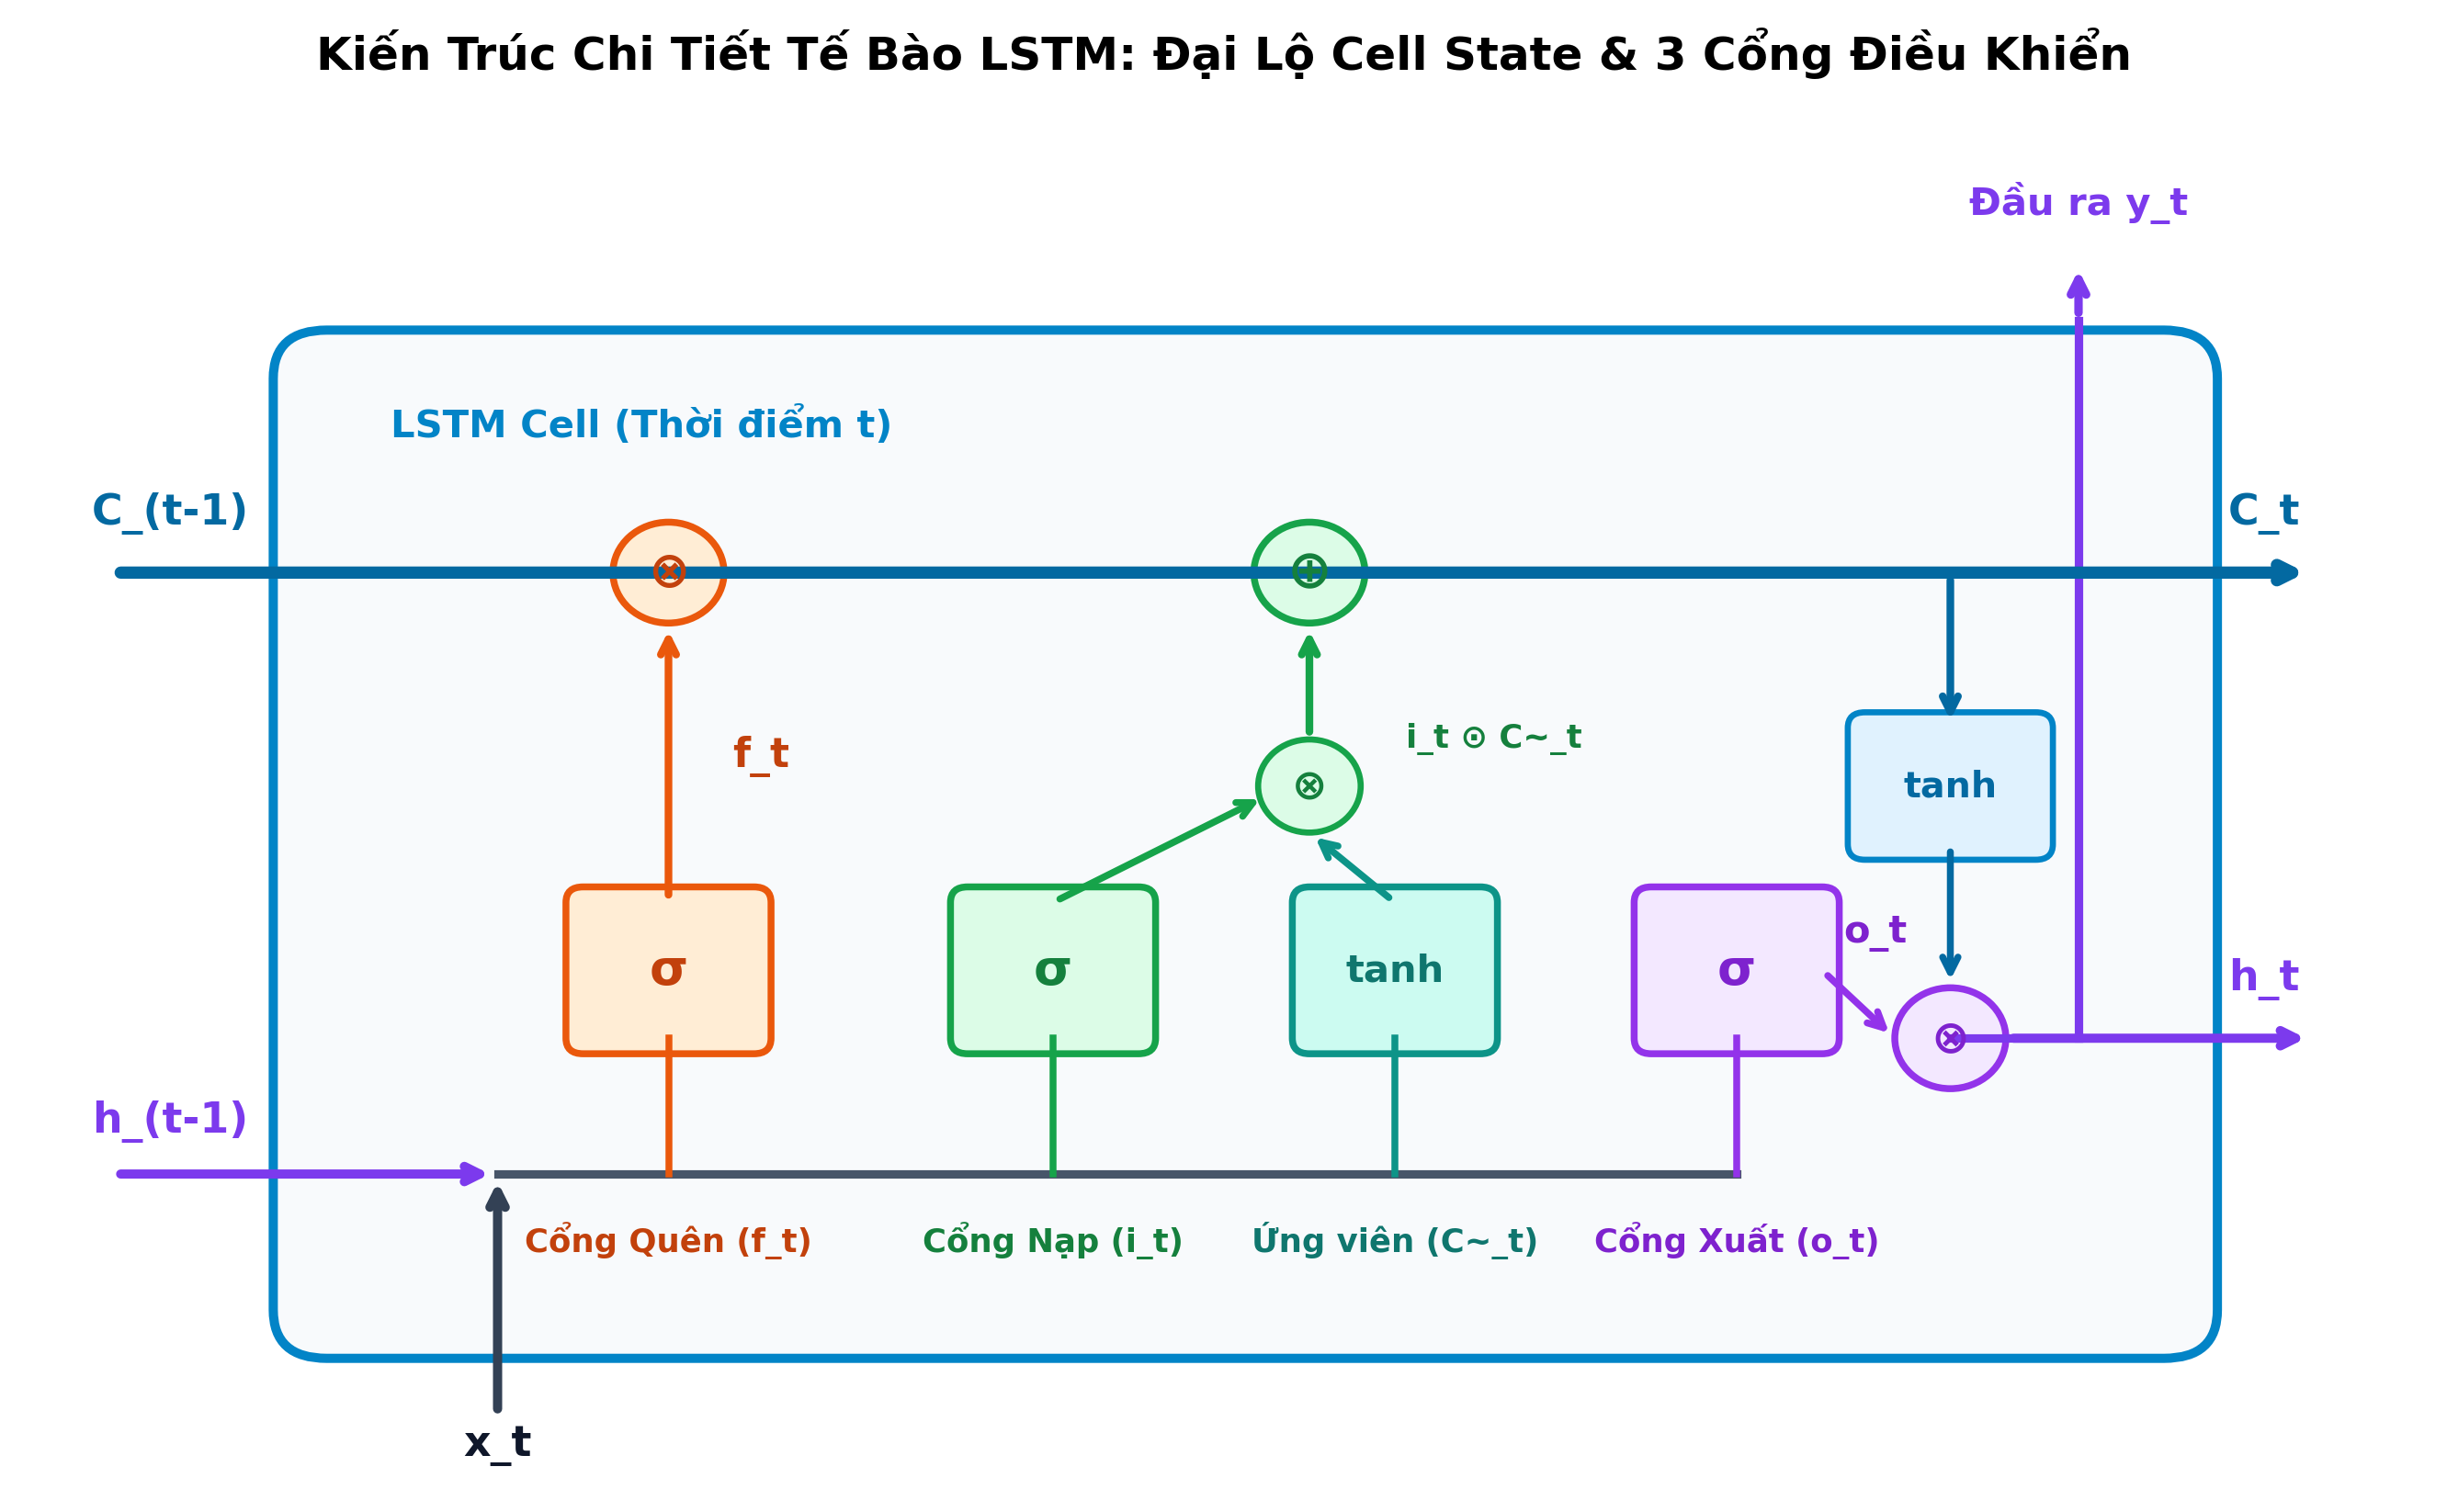
\includegraphics[width=0.88\textwidth]{images/fig605_lstm_cell_architecture.png}
    \caption{Kiến trúc vi mô tế bào LSTM với đường truyền trạng thái ô nhớ (Cell State) và cơ chế điều khiển 3 cổng.}
    \label{fig:rnn_lstm_cell}
\end{figure}

\begin{itemize}[leftmargin=1.2cm]
    \item \textbf{Gated Recurrent Unit (GRU -- Cho et al., 2014):} Tinh gọn hóa kiến trúc LSTM bằng cách hợp nhất Cell State và Hidden State thành một vector trạng thái ẩn duy nhất $\mathbf{h}_t$, sử dụng 2 cổng điều khiển:
    \begin{align}
    \text{Cổng Đặt lại (Reset Gate):} \quad \mathbf{r}_t &= \sigma(\mathbf{W}_r [\mathbf{h}_{t-1}, \mathbf{x}_t] + \mathbf{b}_r) \\
    \text{Cổng Cập nhật (Update Gate):} \quad \mathbf{z}_t &= \sigma(\mathbf{W}_z [\mathbf{h}_{t-1}, \mathbf{x}_t] + \mathbf{b}_z) \\
    \text{Ứng viên Ẩn:} \quad \tilde{\mathbf{h}}_t &= \tanh(\mathbf{W}_h [\mathbf{r}_t \odot \mathbf{h}_{t-1}, \mathbf{x}_t] + \mathbf{b}_h) \\
    \text{Cập nhật Trạng thái:} \quad \mathbf{h}_t &= (1 - \mathbf{z}_t) \odot \mathbf{h}_{t-1} + \mathbf{z}_t \odot \tilde{\mathbf{h}}_t
    \end{align}
    GRU giảm $25\%$ số lượng tham số so với LSTM, giúp giảm thiểu rủi ro quá khớp trên các tập dữ liệu nhỏ và tăng tốc độ hội tụ.
\end{itemize}

\begin{figure}[H]
    \centering
    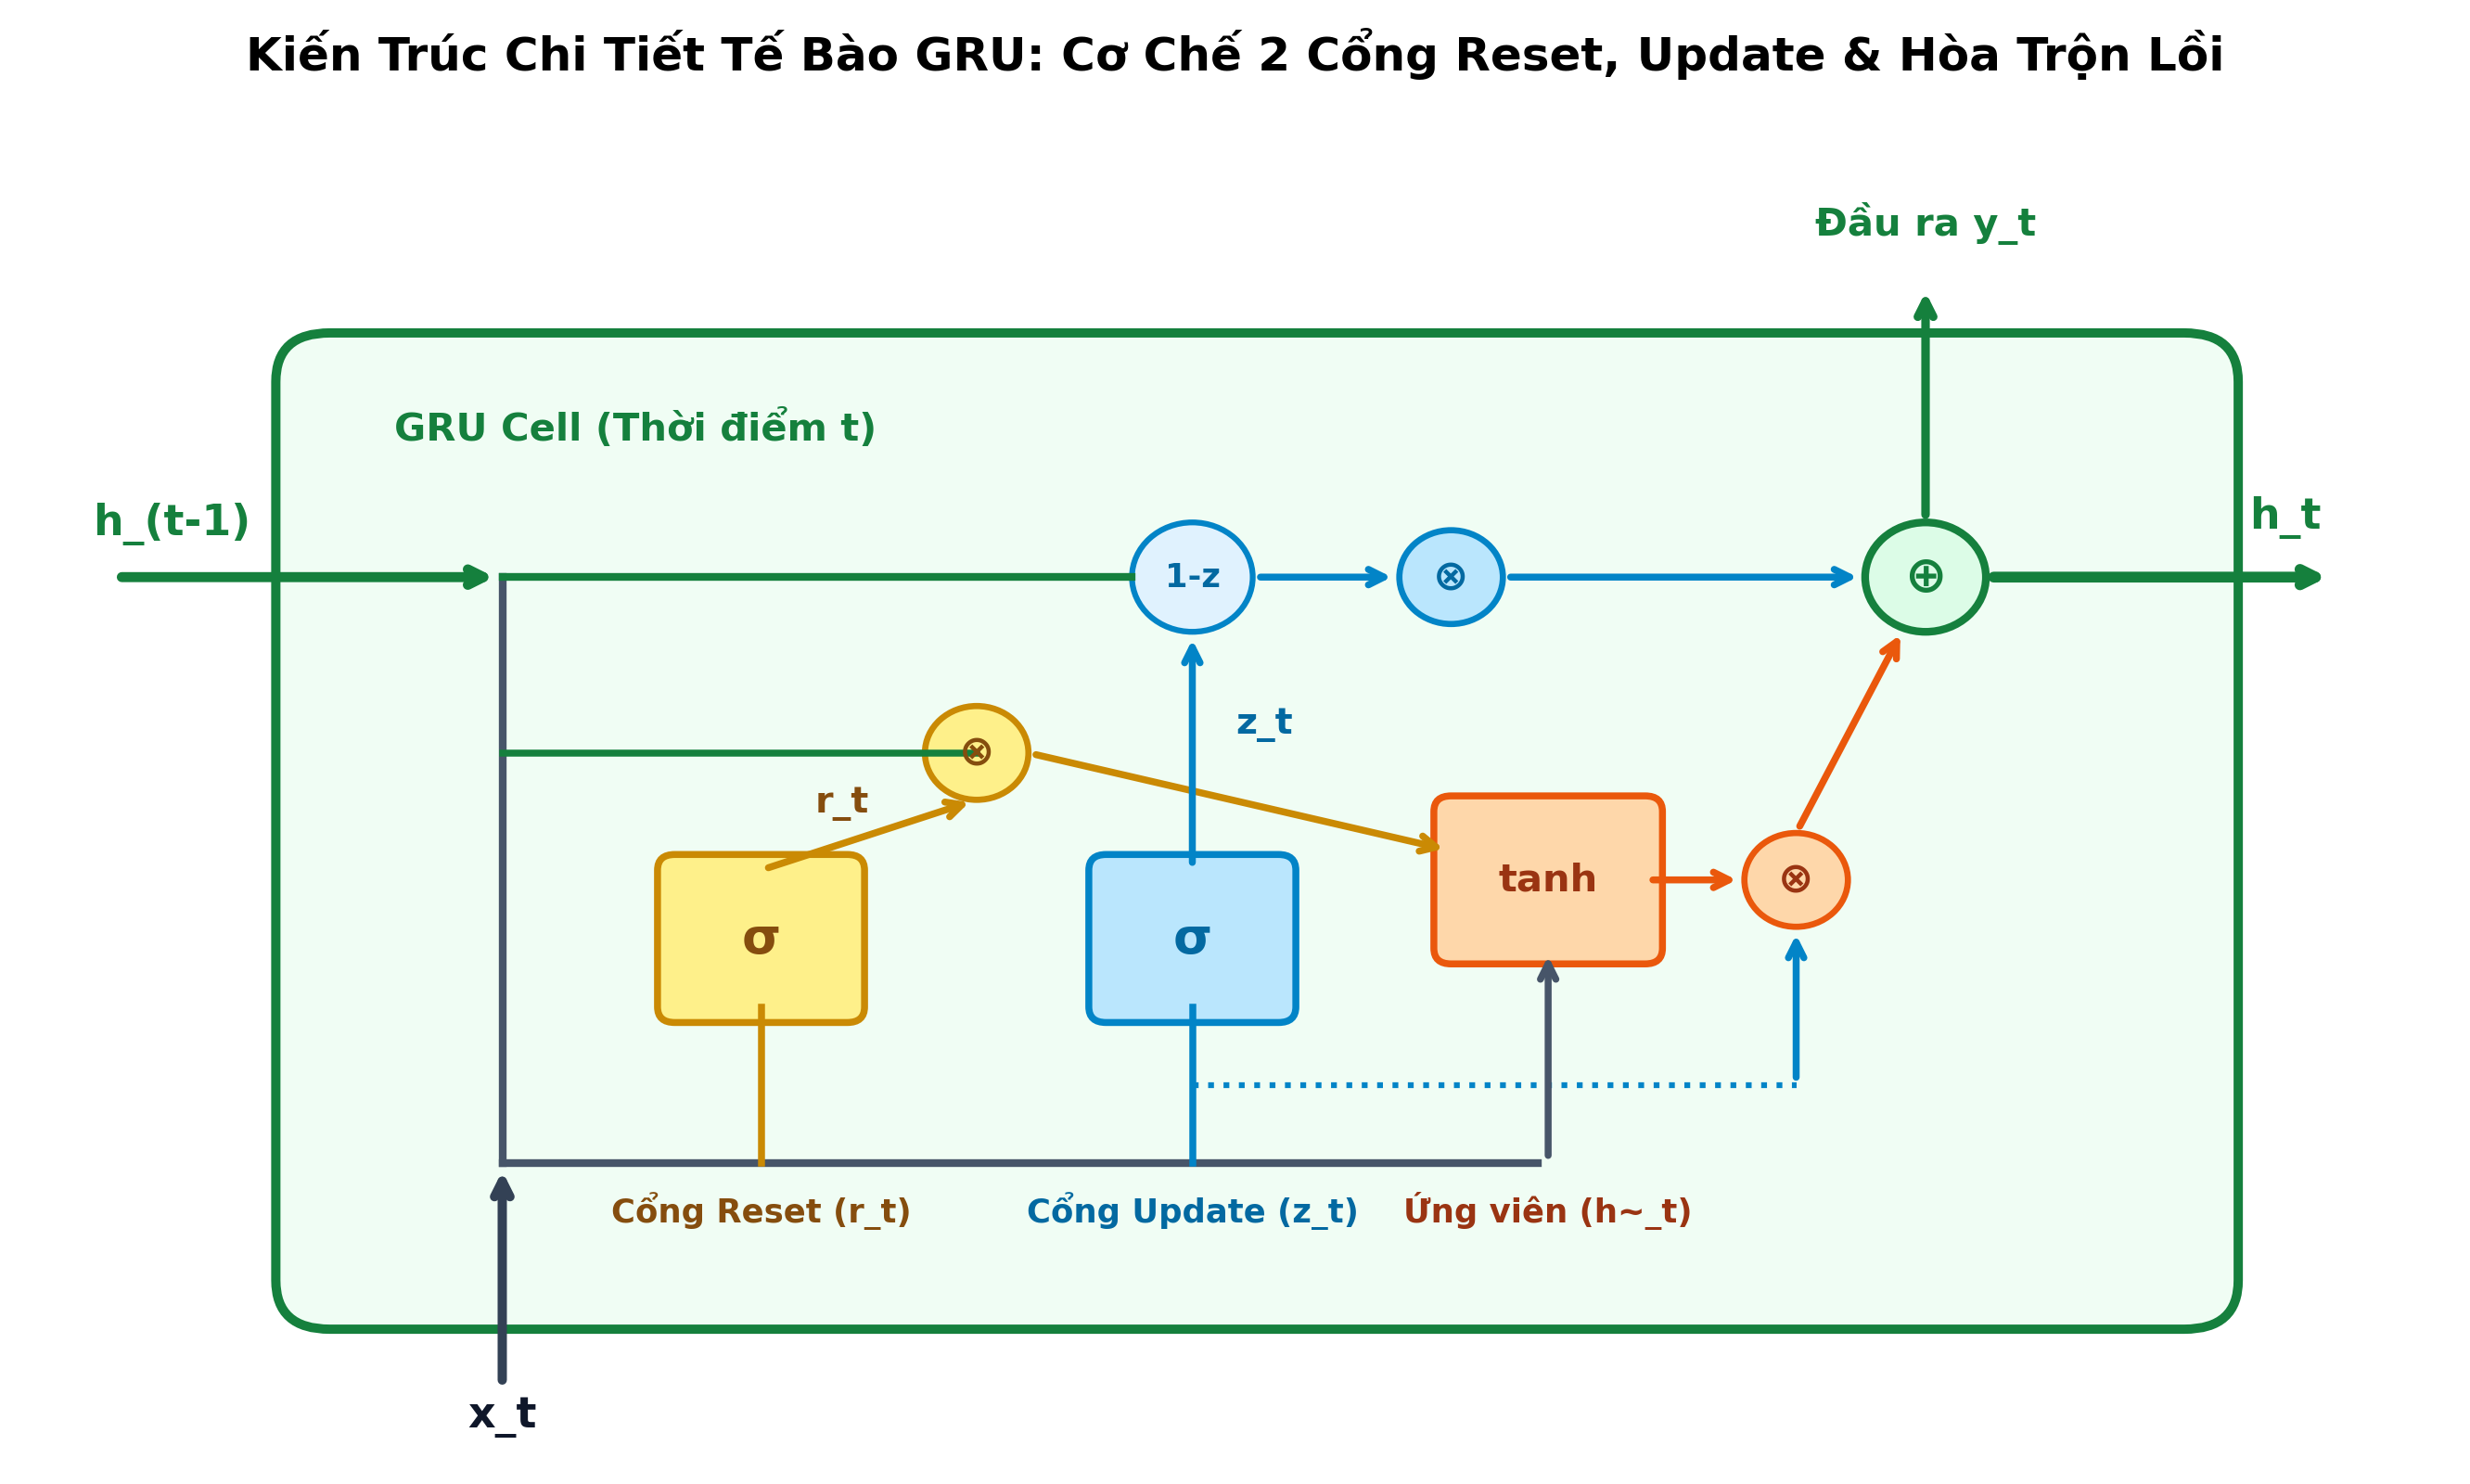
\includegraphics[width=0.88\textwidth]{images/fig606_gru_cell_architecture.png}
    \caption{Kiến trúc vi mô tế bào GRU với cơ chế 2 cổng tích hợp (Update Gate và Reset Gate).}
    \label{fig:rnn_gru_cell}
\end{figure}

\subsection{Mạng Hồi Quy Hai Chiều (BiLSTM) \& Điều Chuẩn Recurrent Dropout}
Trong nhiều bài toán phân tích chuỗi tĩnh (như phân tích quỹ đạo khách hàng hoặc gắn nhãn thực thể), việc tiếp cận cả ngữ cảnh quá khứ lẫn ngữ cảnh tương lai đem lại thông tin phong phú vượt trội. Mạng \textbf{BiLSTM} vận hành đồng thời hai chuỗi độc lập: chuỗi tiến $\overrightarrow{\mathbf{h}}_t$ từ $t=1 \rightarrow T$ và chuỗi lùi $\overleftarrow{\mathbf{h}}_t$ từ $t=T \rightarrow 1$, vector biểu diễn cuối cùng là phép nối ghép: $\mathbf{h}_t = [\overrightarrow{\mathbf{h}}_t, \overleftarrow{\mathbf{h}}_t] \in \mathbb{R}^{2H}$.

\begin{figure}[H]
    \centering
    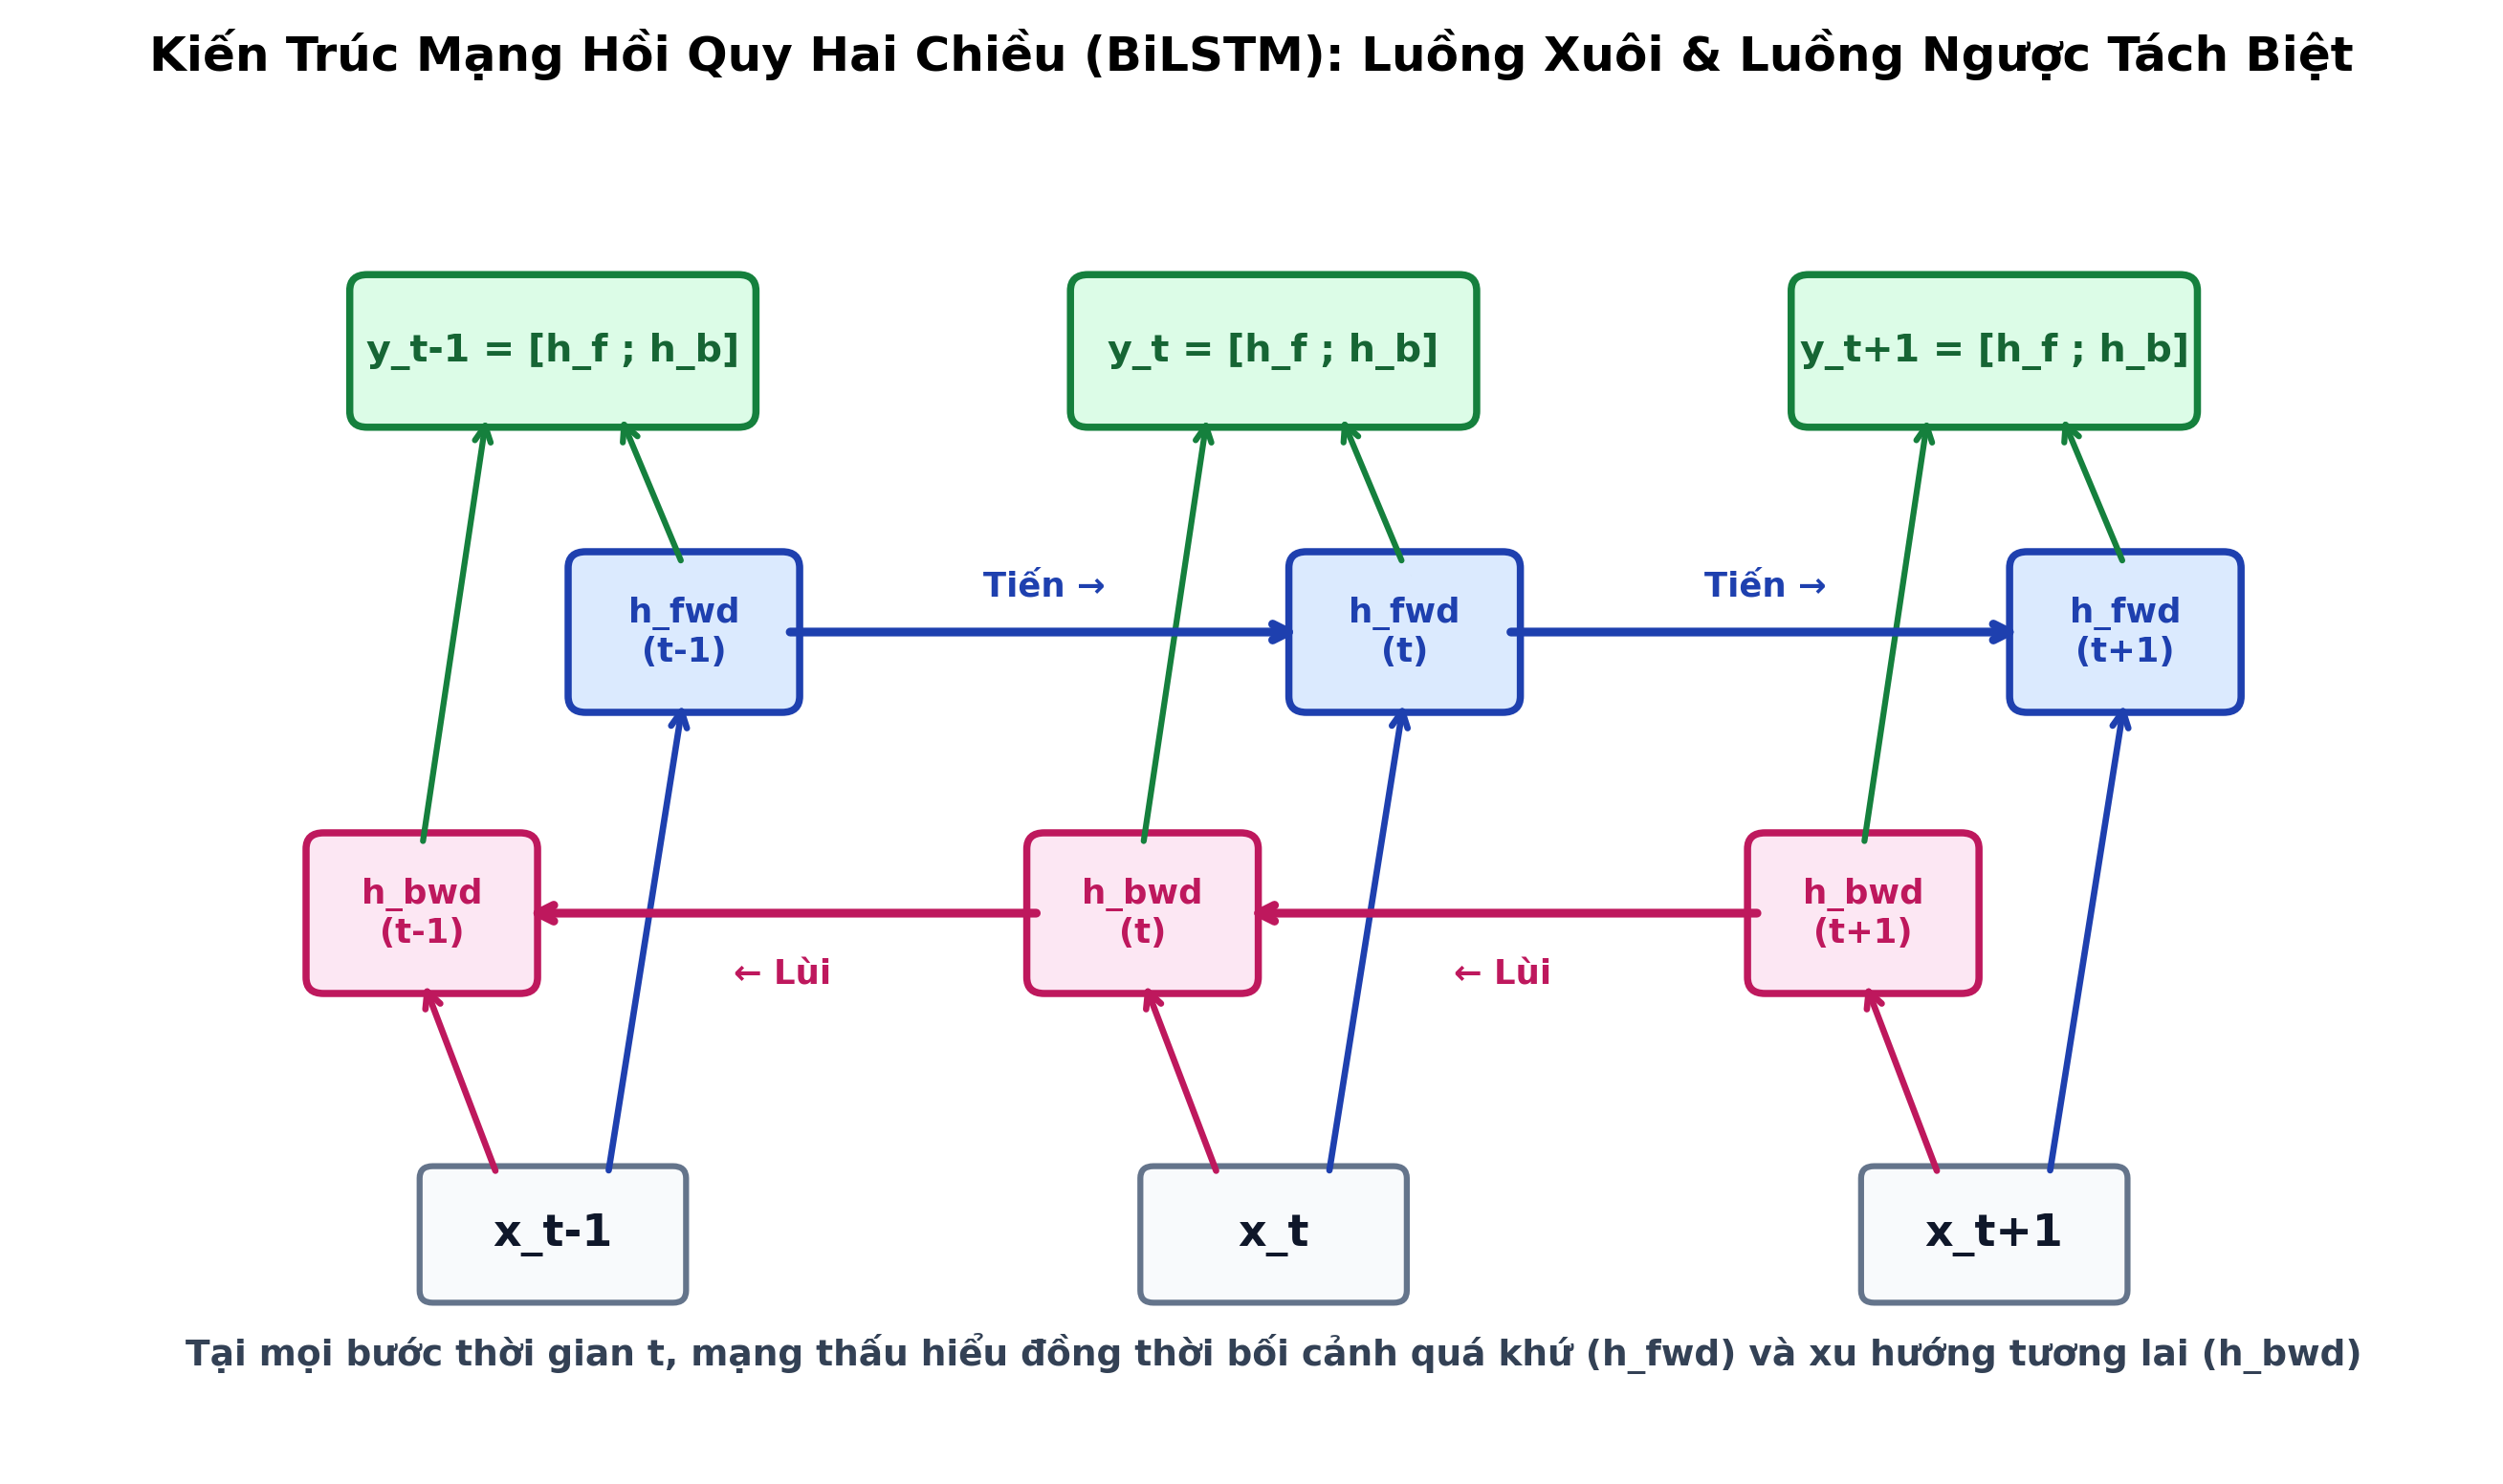
\includegraphics[width=0.88\textwidth]{images/fig607_bidirectional_rnn_architecture.png}
    \caption{Kiến trúc Mạng nơ-ron Hồi quy Hai chiều (Bidirectional RNN / BiLSTM) tổng hợp ngữ cảnh quá khứ và tương lai.}
    \label{fig:rnn_bilstm}
\end{figure}

Đồng thời, việc áp dụng kỹ thuật \textbf{Recurrent Dropout} (Gal \& Ghahramani, 2016) -- sử dụng cùng một mặt nạ nhị phân cố định qua mọi bước thời gian của cùng một mẫu -- giúp điều chuẩn mạng hồi quy hiệu quả mà không làm suy giảm cấu trúc bộ nhớ nội tại.

\begin{figure}[H]
    \centering
    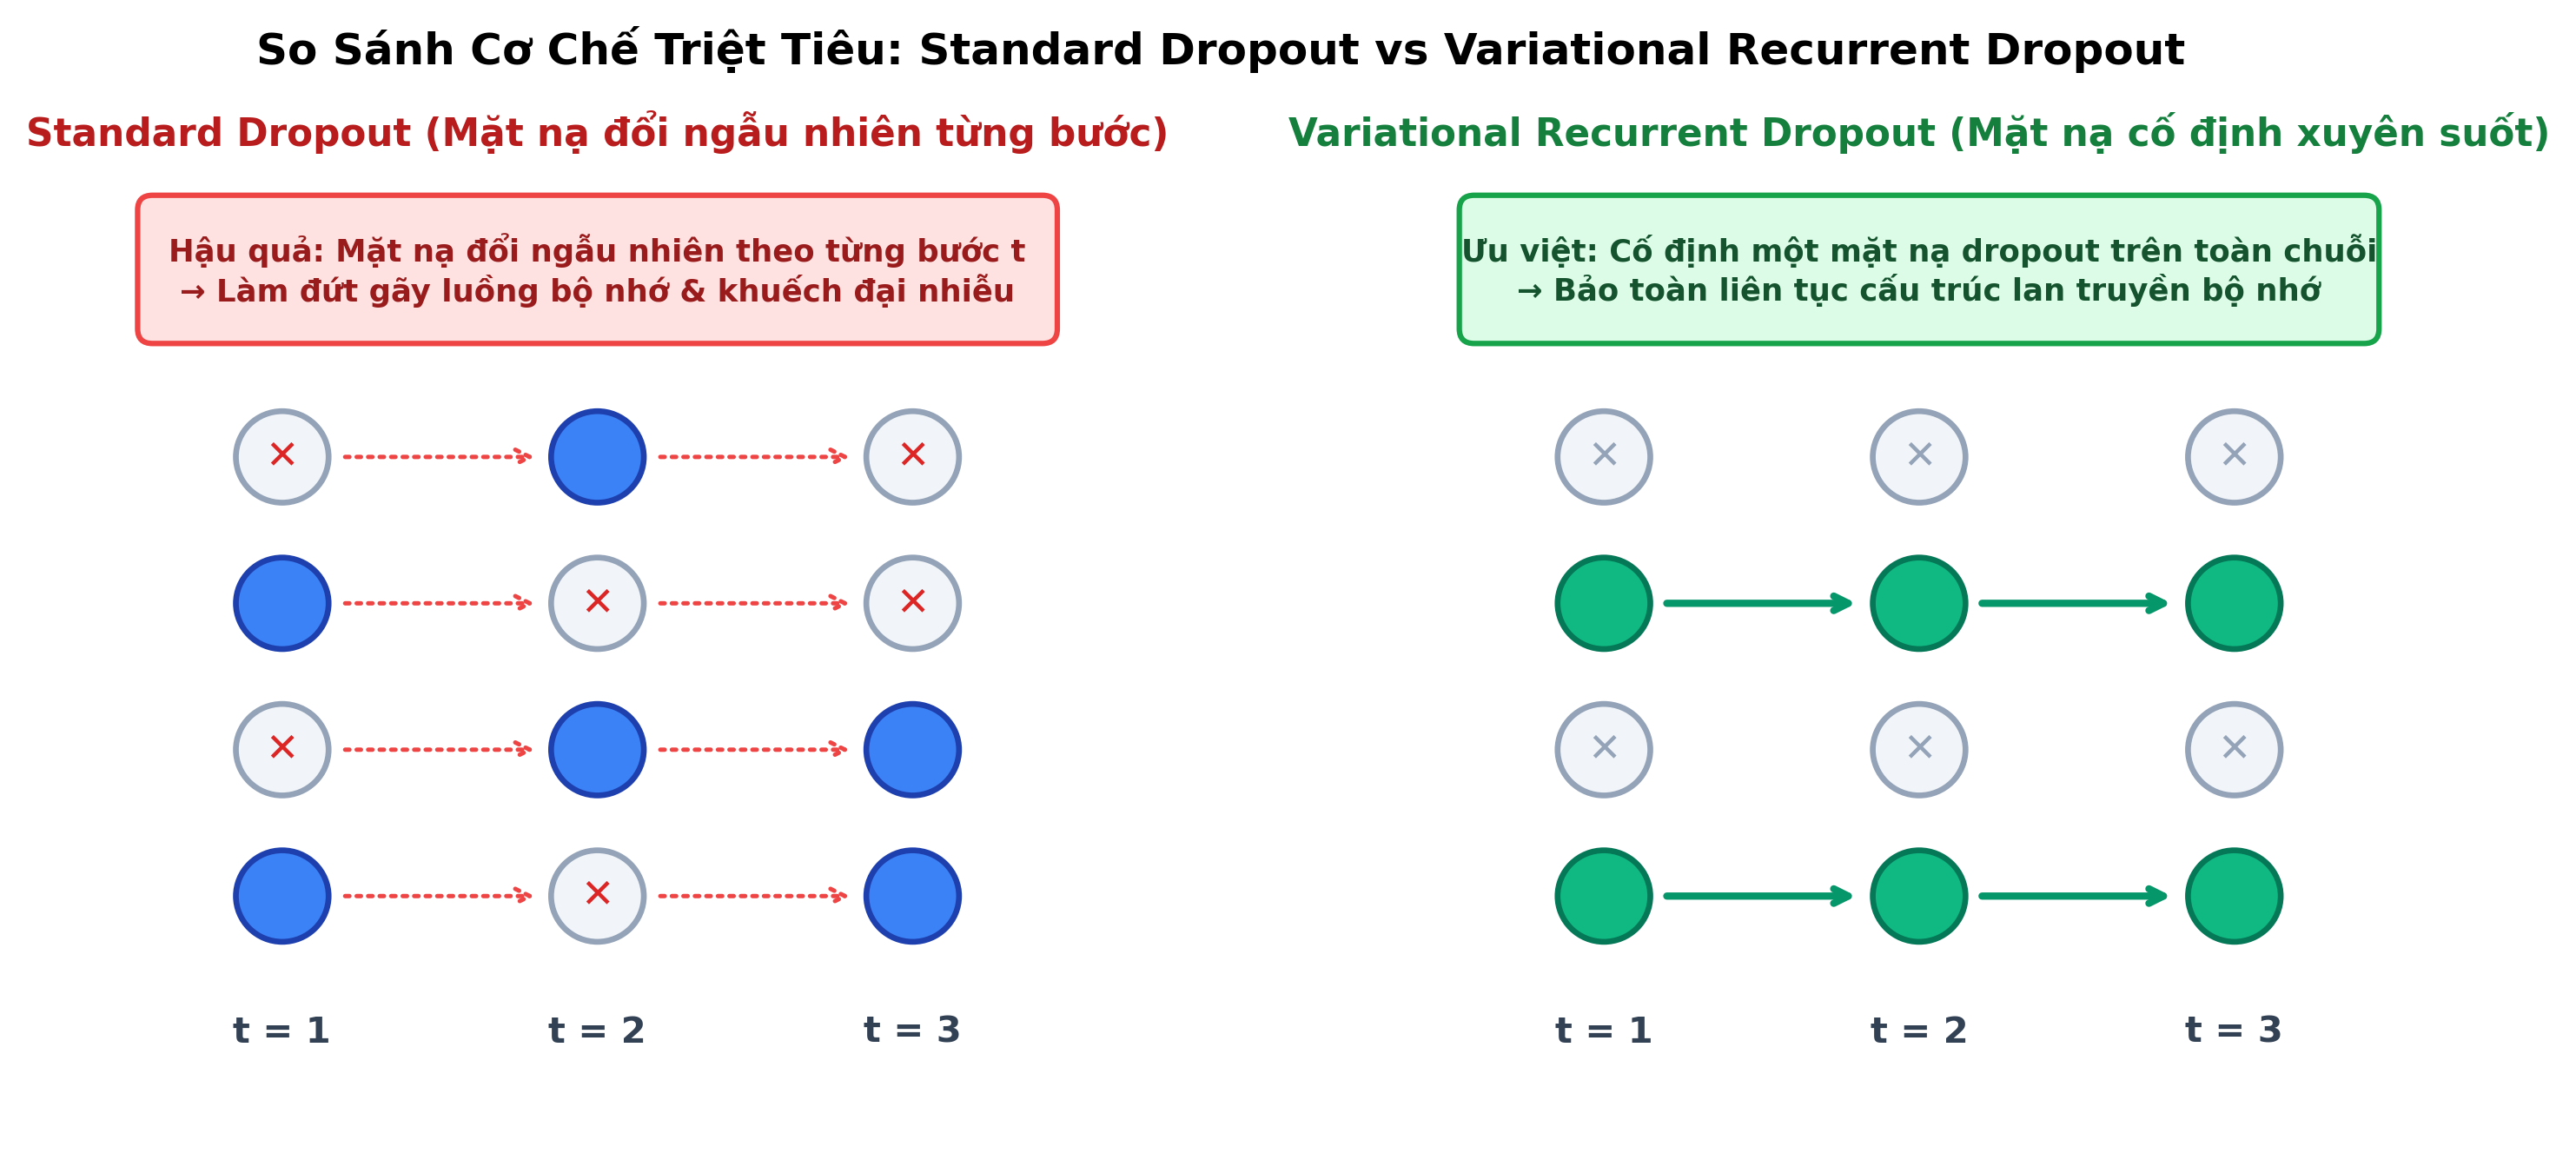
\includegraphics[width=0.86\textwidth]{images/fig608_recurrent_dropout_vs_standard_dropout.png}
    \caption{So sánh giữa Standard Dropout (gây nhiễu bộ nhớ) và Recurrent Dropout (bảo toàn mặt nạ cố định theo thời gian).}
    \label{fig:rnn_dropout}
\end{figure}

\section{Khảo Sát Thực Nghiệm và Tiền Xử Lý 2 Bộ Dữ Liệu Chuỗi Lớn}

\subsection{Tập Dữ Liệu 1: Chuỗi Thời Gian Chứng Khoán Việt Nam (VN30 / HoSE 2012 -- 2026)}
\begin{itemize}[leftmargin=1.2cm]
    \item \textbf{Nguồn gốc dữ liệu:} Lịch sử giao dịch tài chính các mã cổ phiếu trụ cột thuộc rổ chỉ số VN30 niêm yết trên Sở Giao dịch Chứng khoán TP.HCM (HoSE) thu thập từ Yahoo Finance (\url{https://finance.yahoo.com/quote/FPT.VN/history}), bao gồm 4 doanh nghiệp đầu ngành đại diện cho các trụ cột kinh tế: FPT (Công nghệ - Viễn thông), VCB (Ngân hàng TMCP Ngoại thương Việt Nam), HPG (Tập đoàn Hòa Phát - Thép \& Công nghiệp nặng), và VIC (Tập đoàn Vingroup - Bất động sản \& Dịch vụ).
    \item \textbf{Quy mô và chiều dữ liệu:} Gồm tổng cộng $15,225$ phiên giao dịch liên tục suốt 14 năm (từ tháng 01/2012 đến tháng 09/2026), trong đó riêng mã FPT có $3,825$ phiên, VCB có $3,816$ phiên, HPG có $3,825$ phiên và VIC có $3,759$ phiên. Sau khi trích xuất các chỉ báo kỹ thuật tài chính động, tập dữ liệu có $8$ đặc trưng quan sát tại mỗi phiên: Giá mở cửa (Open), Giá cao nhất (High), Giá thấp nhất (Low), Giá đóng cửa (Close), Khối lượng giao dịch (Volume), Trung bình trượt 20 ngày (SMA20), Trung bình trượt 50 ngày (SMA50), Chỉ số sức mạnh tương đối 14 ngày (RSI-14), và Độ biến động 30 ngày (Volatility-30d).
\end{itemize}

\begin{table}[H]
\centering
\small
\caption{Trích xuất 5 phiên giao dịch tiêu biểu kèm chỉ báo kỹ thuật của cổ phiếu FPT (FPT.VN) trên sàn HoSE}
\label{tab:sample_vn_stock}
\begin{tabularx}{\textwidth}{>{\centering\arraybackslash}p{2.2cm} >{\centering\arraybackslash}X >{\centering\arraybackslash}X >{\centering\arraybackslash}X >{\centering\arraybackslash}X >{\centering\arraybackslash}X >{\centering\arraybackslash}X >{\centering\arraybackslash}X}
\toprule
\textbf{Ngày} & \textbf{Open (VNĐ)} & \textbf{High (VNĐ)} & \textbf{Low (VNĐ)} & \textbf{Close (VNĐ)} & \textbf{Volume (CP)} & \textbf{SMA20} & \textbf{RSI-14} \\
\midrule
09/03/2012 & 4,254 & 4,368 & 4,254 & 4,292 & 1,505,570 & 4,138 & 69.23 \\
22/10/2015 & 7,559 & 7,608 & 7,559 & 7,575 & 2,103,678 & 7,390 & 70.91 \\
02/07/2019 & 14,867 & 15,026 & 14,757 & 14,836 & 4,248,729 & 14,296 & 63.31 \\
17/02/2023 & 45,143 & 45,365 & 45,032 & 45,365 & 782,277 & 45,613 & 32.79 \\
30/09/2026 & 63,400 & 64,000 & 63,000 & 63,000 & 3,041,400 & 65,602 & 27.74 \\
\bottomrule
\end{tabularx}
\end{table}

\begin{figure}[H]
    \centering
    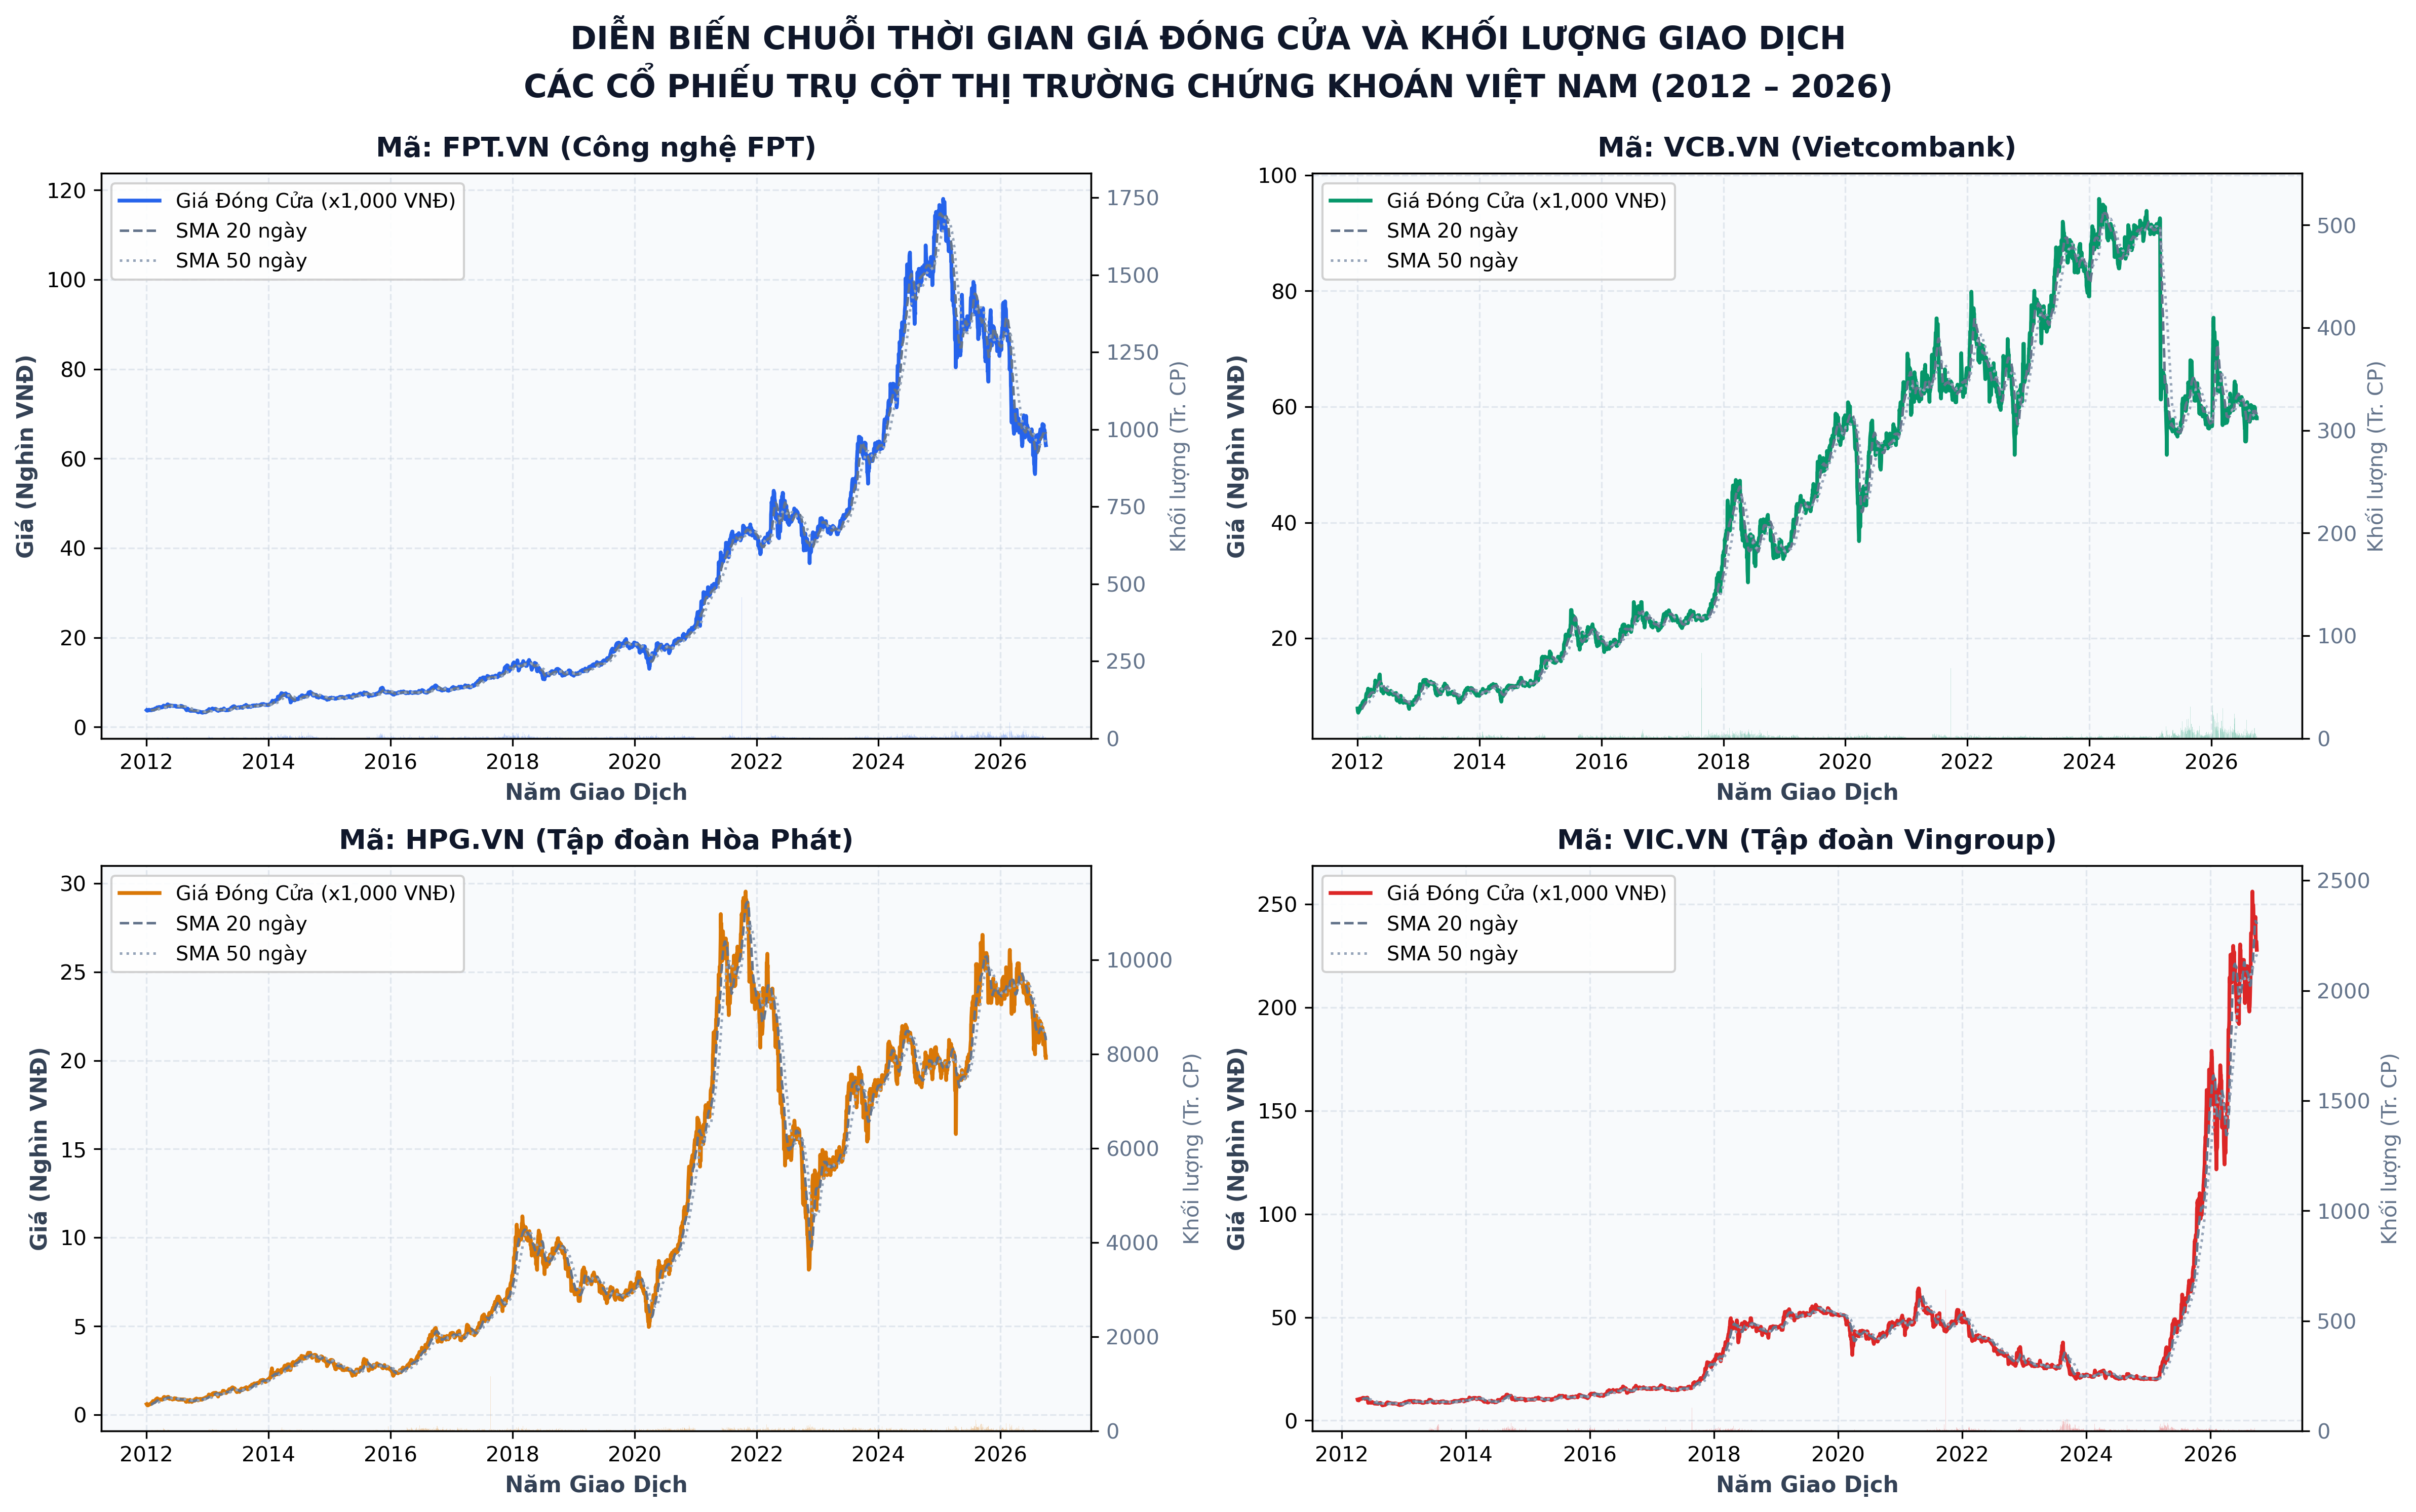
\includegraphics[width=\textwidth]{images/fig609_vn_stock_eda_timeseries.png}
    \caption{Diễn biến chuỗi thời gian giá đóng cửa và khối lượng giao dịch các cổ phiếu trụ cột VN30 (FPT, VCB, HPG, VIC) giai đoạn 2012 -- 2026 và các đường trung bình động SMA.}
    \label{fig:vn_stock_eda}
\end{figure}

\begin{figure}[H]
    \centering
    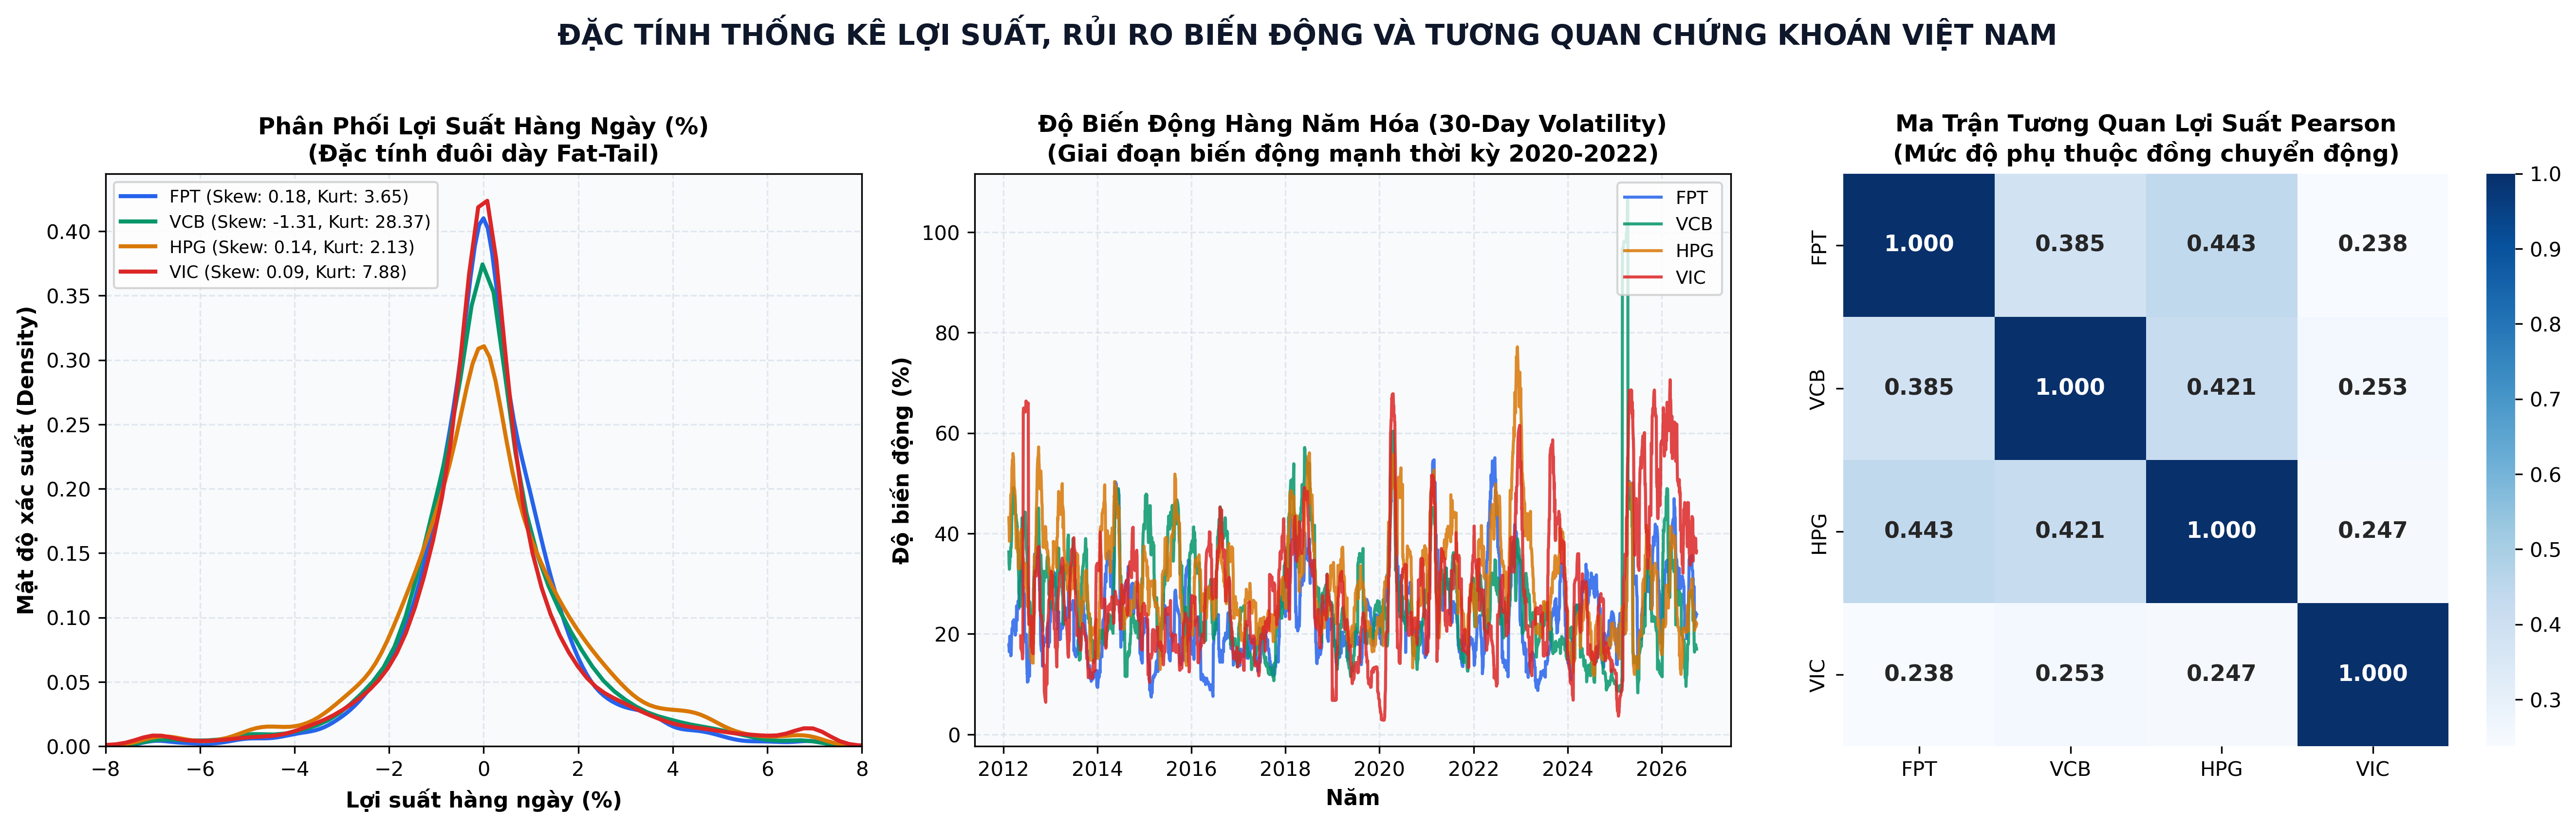
\includegraphics[width=\textwidth]{images/fig609b_vn_stock_distributions_volatility_and_correlation.png}
    \caption{Phân phối lợi suất hàng ngày (KDE), độ biến động 30 ngày (Rolling Volatility) và ma trận tương quan Pearson giữa 4 mã trụ cột thị trường chứng khoán Việt Nam.}
    \label{fig:vn_stock_volatility}
\end{figure}

\begin{figure}[H]
    \centering
    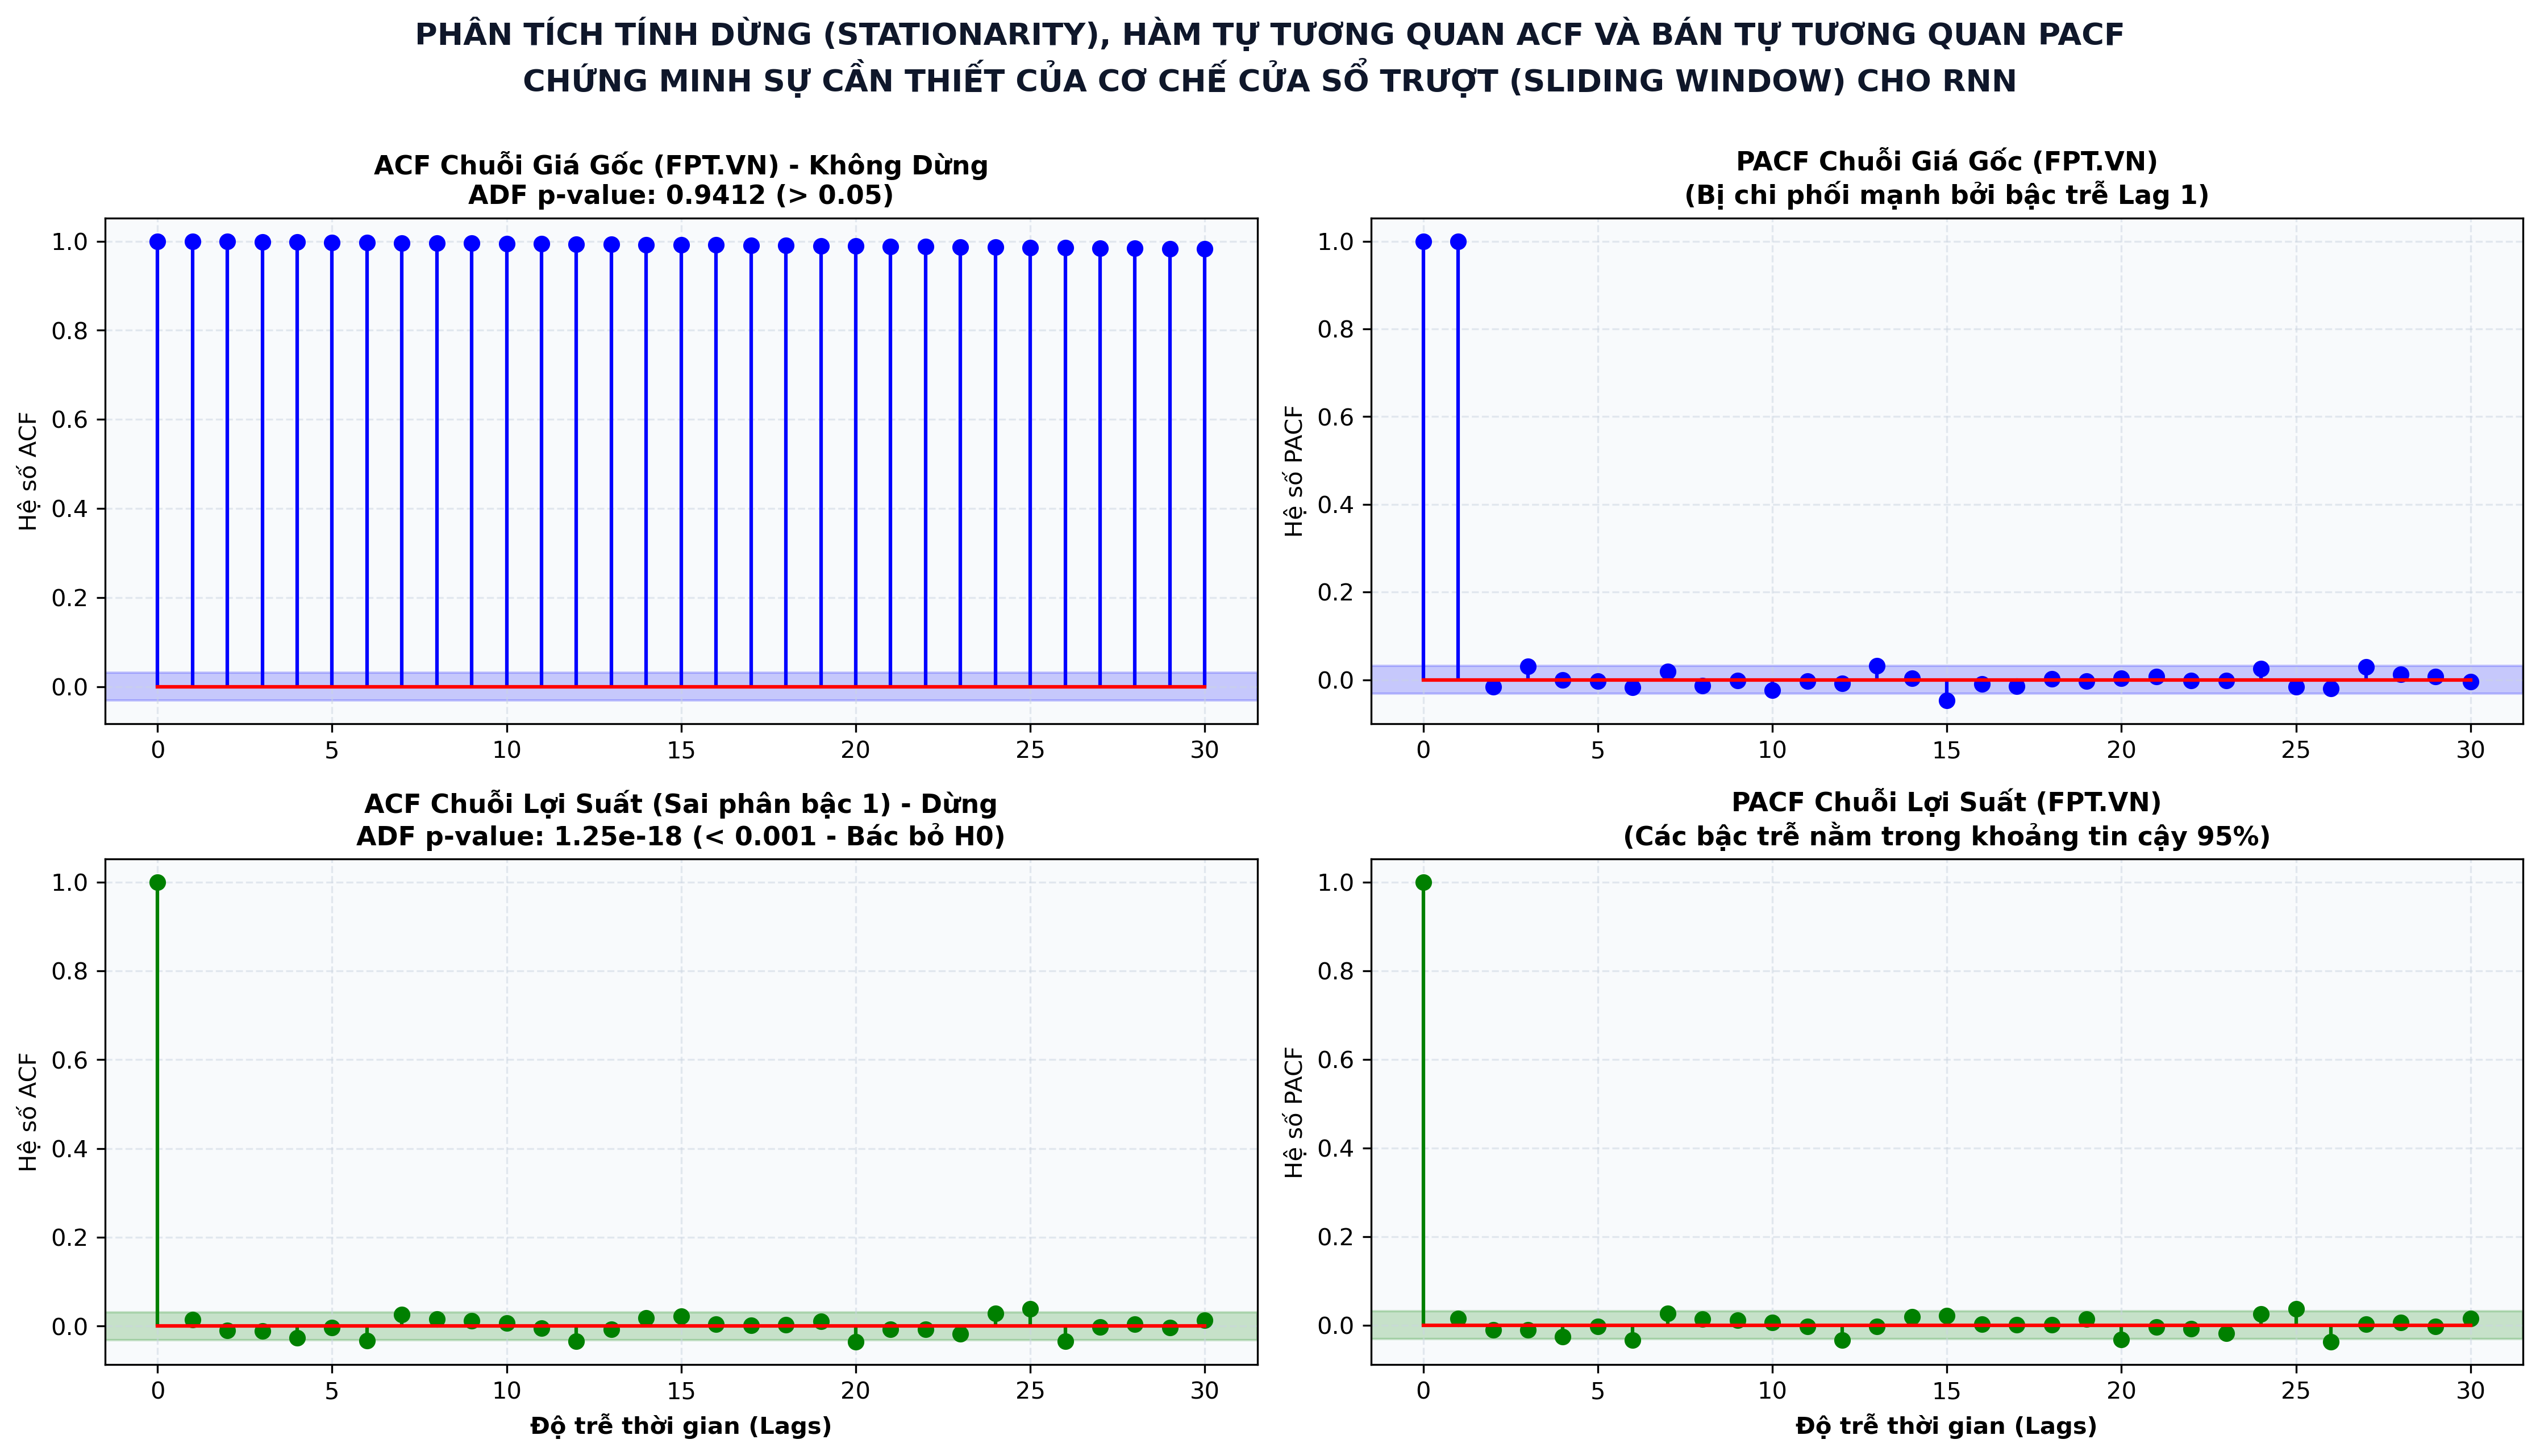
\includegraphics[width=0.92\textwidth]{images/fig610_vn_stock_acf_pacf_stationarity.png}
    \caption{Đồ thị Hàm tự tương quan (ACF), Tự tương quan riêng phần (PACF) và kiểm định nghiệm đơn vị Augmented Dickey-Fuller (ADF) khẳng định tính chất phụ thuộc trễ dài hạn của cổ phiếu FPT.VN.}
    \label{fig:vn_stock_acf}
\end{figure}

\begin{figure}[H]
    \centering
    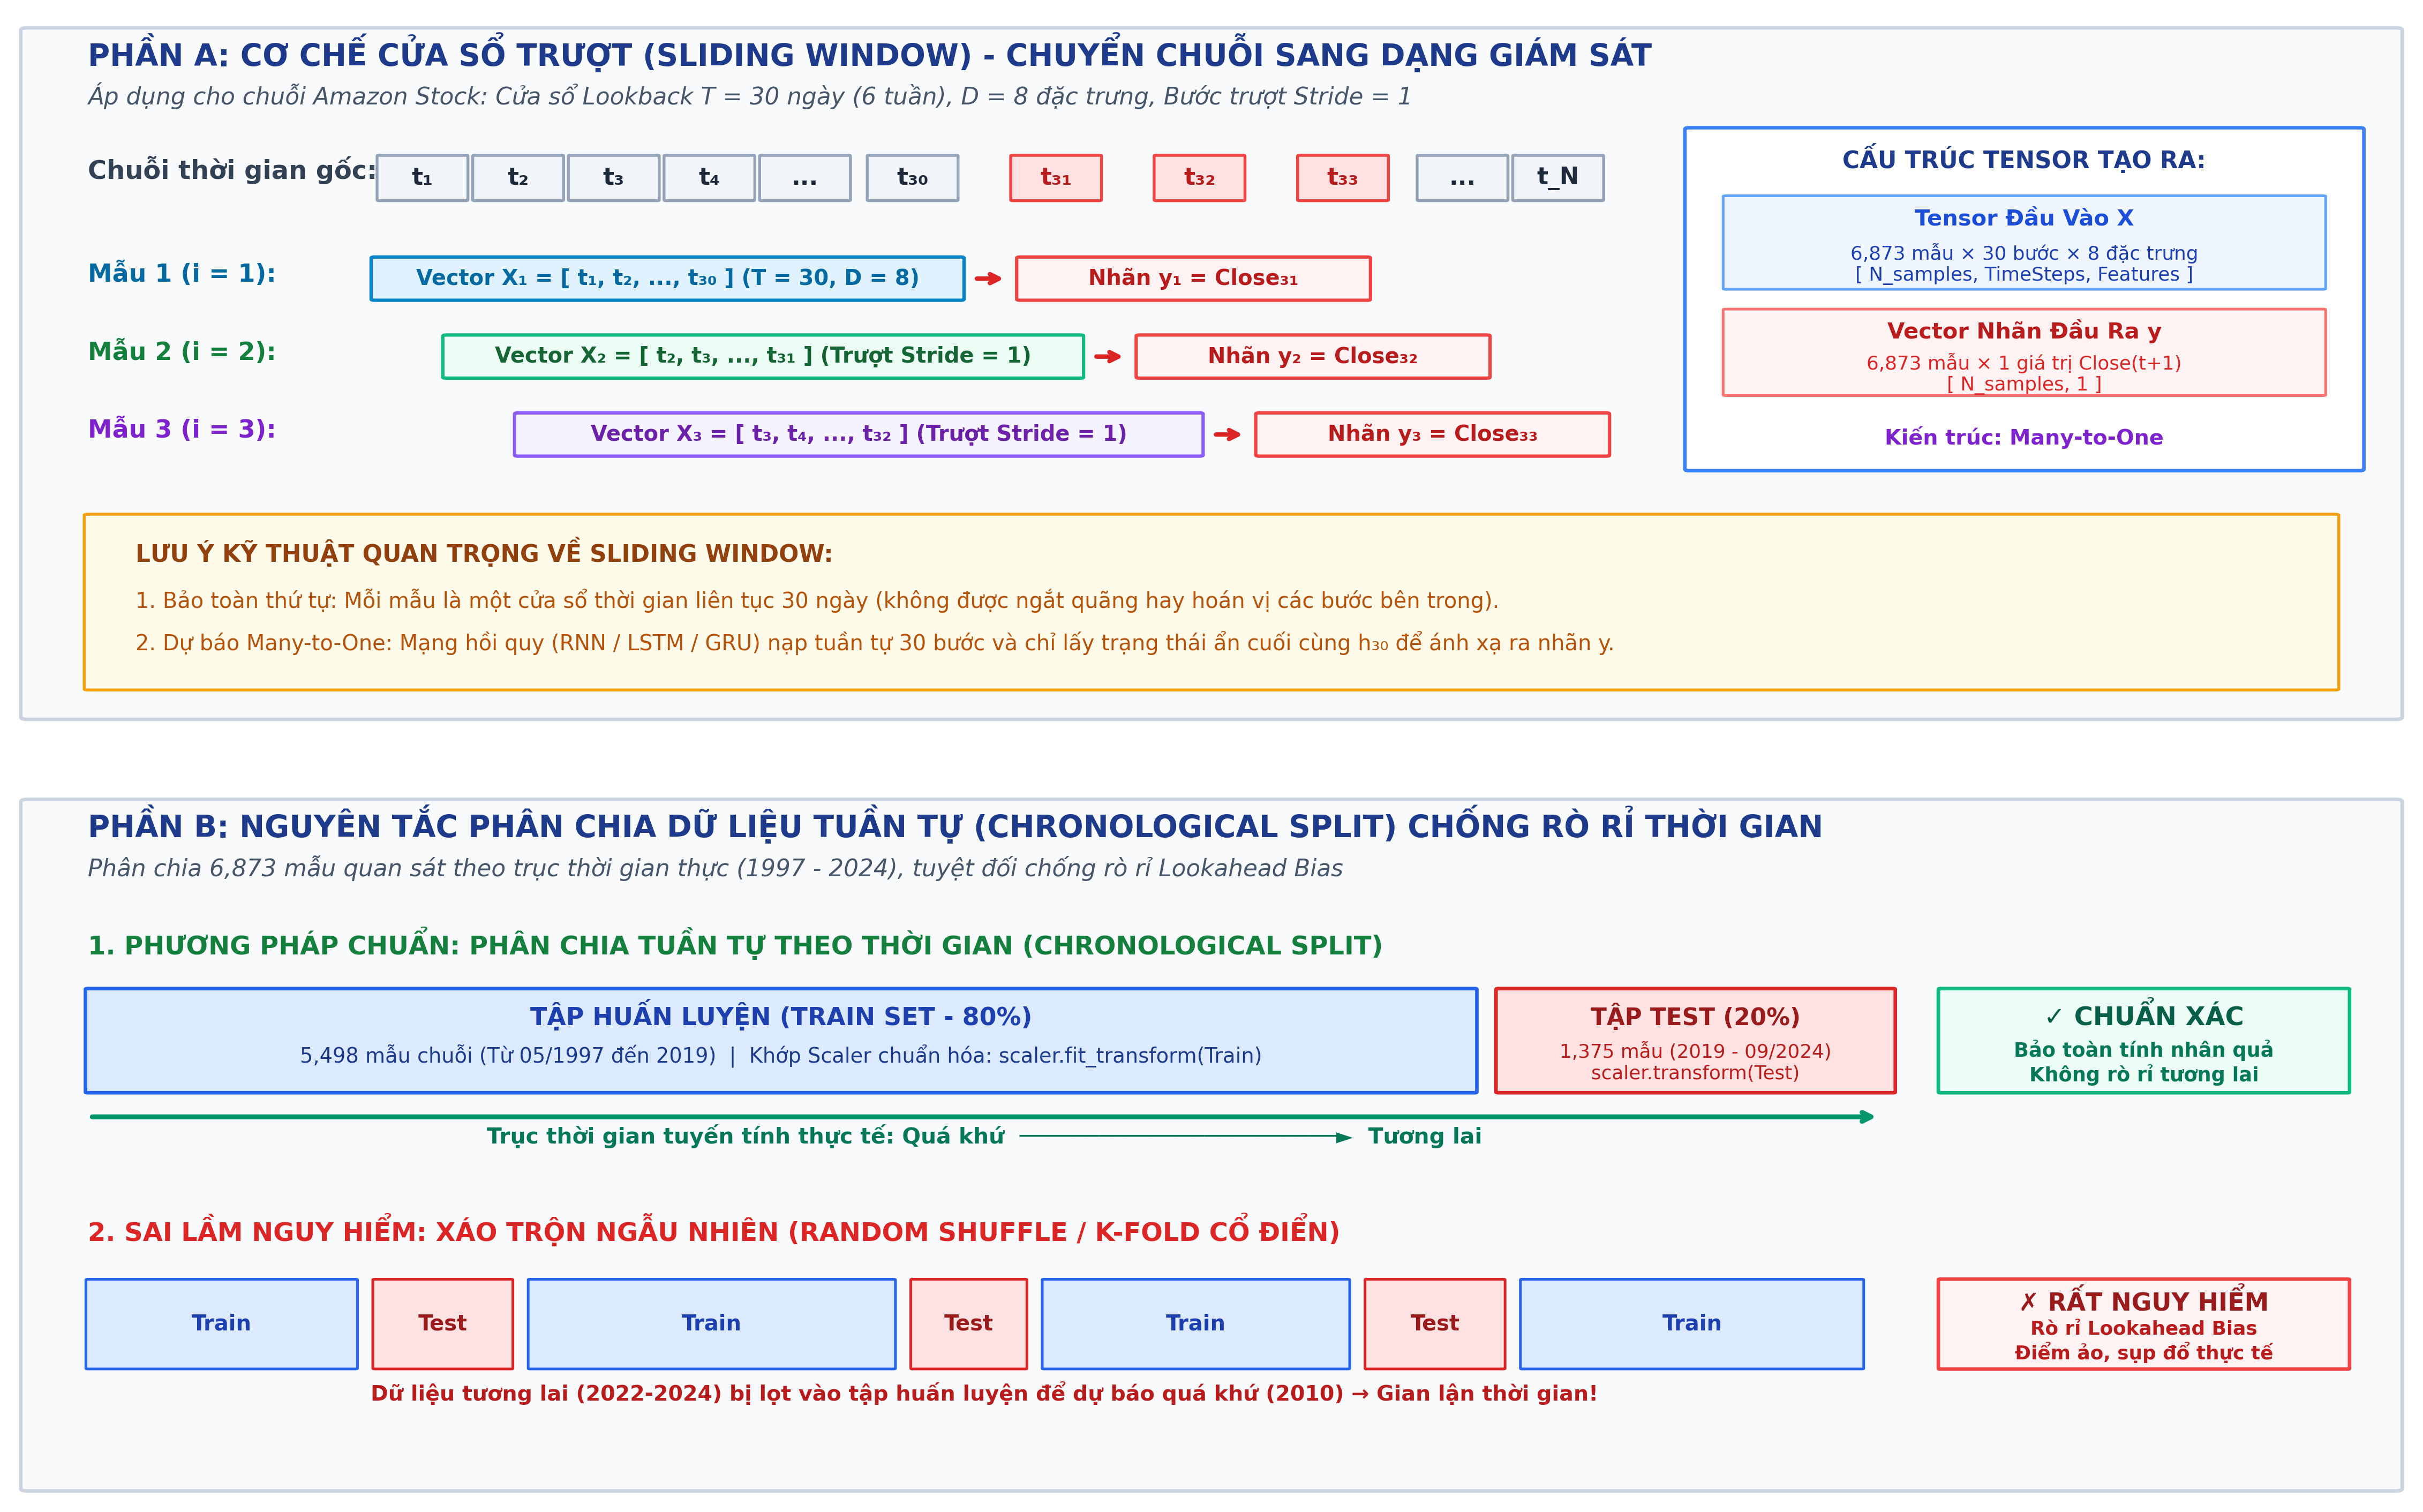
\includegraphics[width=\textwidth]{images/fig611_sliding_window_mechanism.png}
    \caption{Cơ chế tạo mẫu Cửa sổ trượt (Sliding Window Lookback $T = 30$) và nguyên tắc phân chia tuần tự (Chronological Split) chống rò rỉ thời gian (Lookahead Bias).}
    \label{fig:sliding_window}
\end{figure}

\noindent \textbf{Nguyên tắc tiền xử lý chuỗi thời gian chuẩn xác:}
\begin{enumerate}[leftmargin=1.2cm]
    \item \textbf{Cơ chế Cửa sổ trượt (Sliding Window):} Với chuỗi cổ phiếu FPT.VN, độ dài nhìn lại (Lookback) $T = 30$ ngày và bước trượt Stride $= 1$, chuỗi dữ liệu gốc được biến đổi thành $3,746$ mẫu tensor đầu vào $\mathbf{X}_i \in \mathbb{R}^{30 \times 8}$ để dự báo giá đóng cửa phiên kế tiếp $y_i = \text{Close}_{t+1}$.
    \item \textbf{Phân chia tuần tự chống rò rỉ thông tin (Lookahead Bias):} Tuyệt đối không sử dụng phương pháp xáo trộn ngẫu nhiên (random shuffle) vì sẽ làm dữ liệu tương lai lọt vào tập huấn luyện của quá khứ. Toàn bộ chuỗi được phân chia nghiêm ngặt theo trục thời gian thực: Tập Huấn luyện ($80\%$ -- $2,996$ mẫu từ năm 2012 đến đầu năm 2023) và Tập Kiểm thử ($20\%$ -- $750$ mẫu từ năm 2023 đến 09/2026). Bộ chuẩn hóa \texttt{MinMaxScaler} chỉ được khớp (\texttt{fit}) trên tập Train và áp dụng (\texttt{transform}) sang tập Test.
\end{enumerate}

\subsection{Tập Dữ Liệu 2: Quỹ Đạo Hành Vi Khách Hàng (Customer Sequential Behavior)}
\begin{itemize}[leftmargin=1.2cm]
    \item \textbf{Nguồn gốc dữ liệu:} Bộ dữ liệu hành vi người dùng dịch vụ thuê bao số (Subscription E-Commerce / SaaS) mô phỏng từ các nền tảng thương mại thực tế.
    \item \textbf{Quy mô và chiều dữ liệu:} Gồm $60,000$ bản ghi chuỗi tương ứng với $5,000$ khách hàng độc lập được theo dõi quỹ đạo liên tục trong suốt 12 tháng ($T = 12$). Mỗi bước tháng thu thập $8$ chiều hành vi động: Tần suất đăng nhập (Login Frequency), Số đơn hàng (Purchase Count), Số vé yêu cầu hỗ trợ (Support Tickets), Thời lượng sử dụng (Session Duration), Cước phí hàng tháng (Monthly Charges), Số ngày quá hạn thanh toán (Overdue Days), Điểm tương tác (Engagement Score), và Nhãn mục tiêu là Rủi ro khách hàng rời bỏ dịch vụ (Churn: $1$ -- Rời bỏ, $0$ -- Duy trì).
\end{itemize}

\begin{figure}[H]
    \centering
    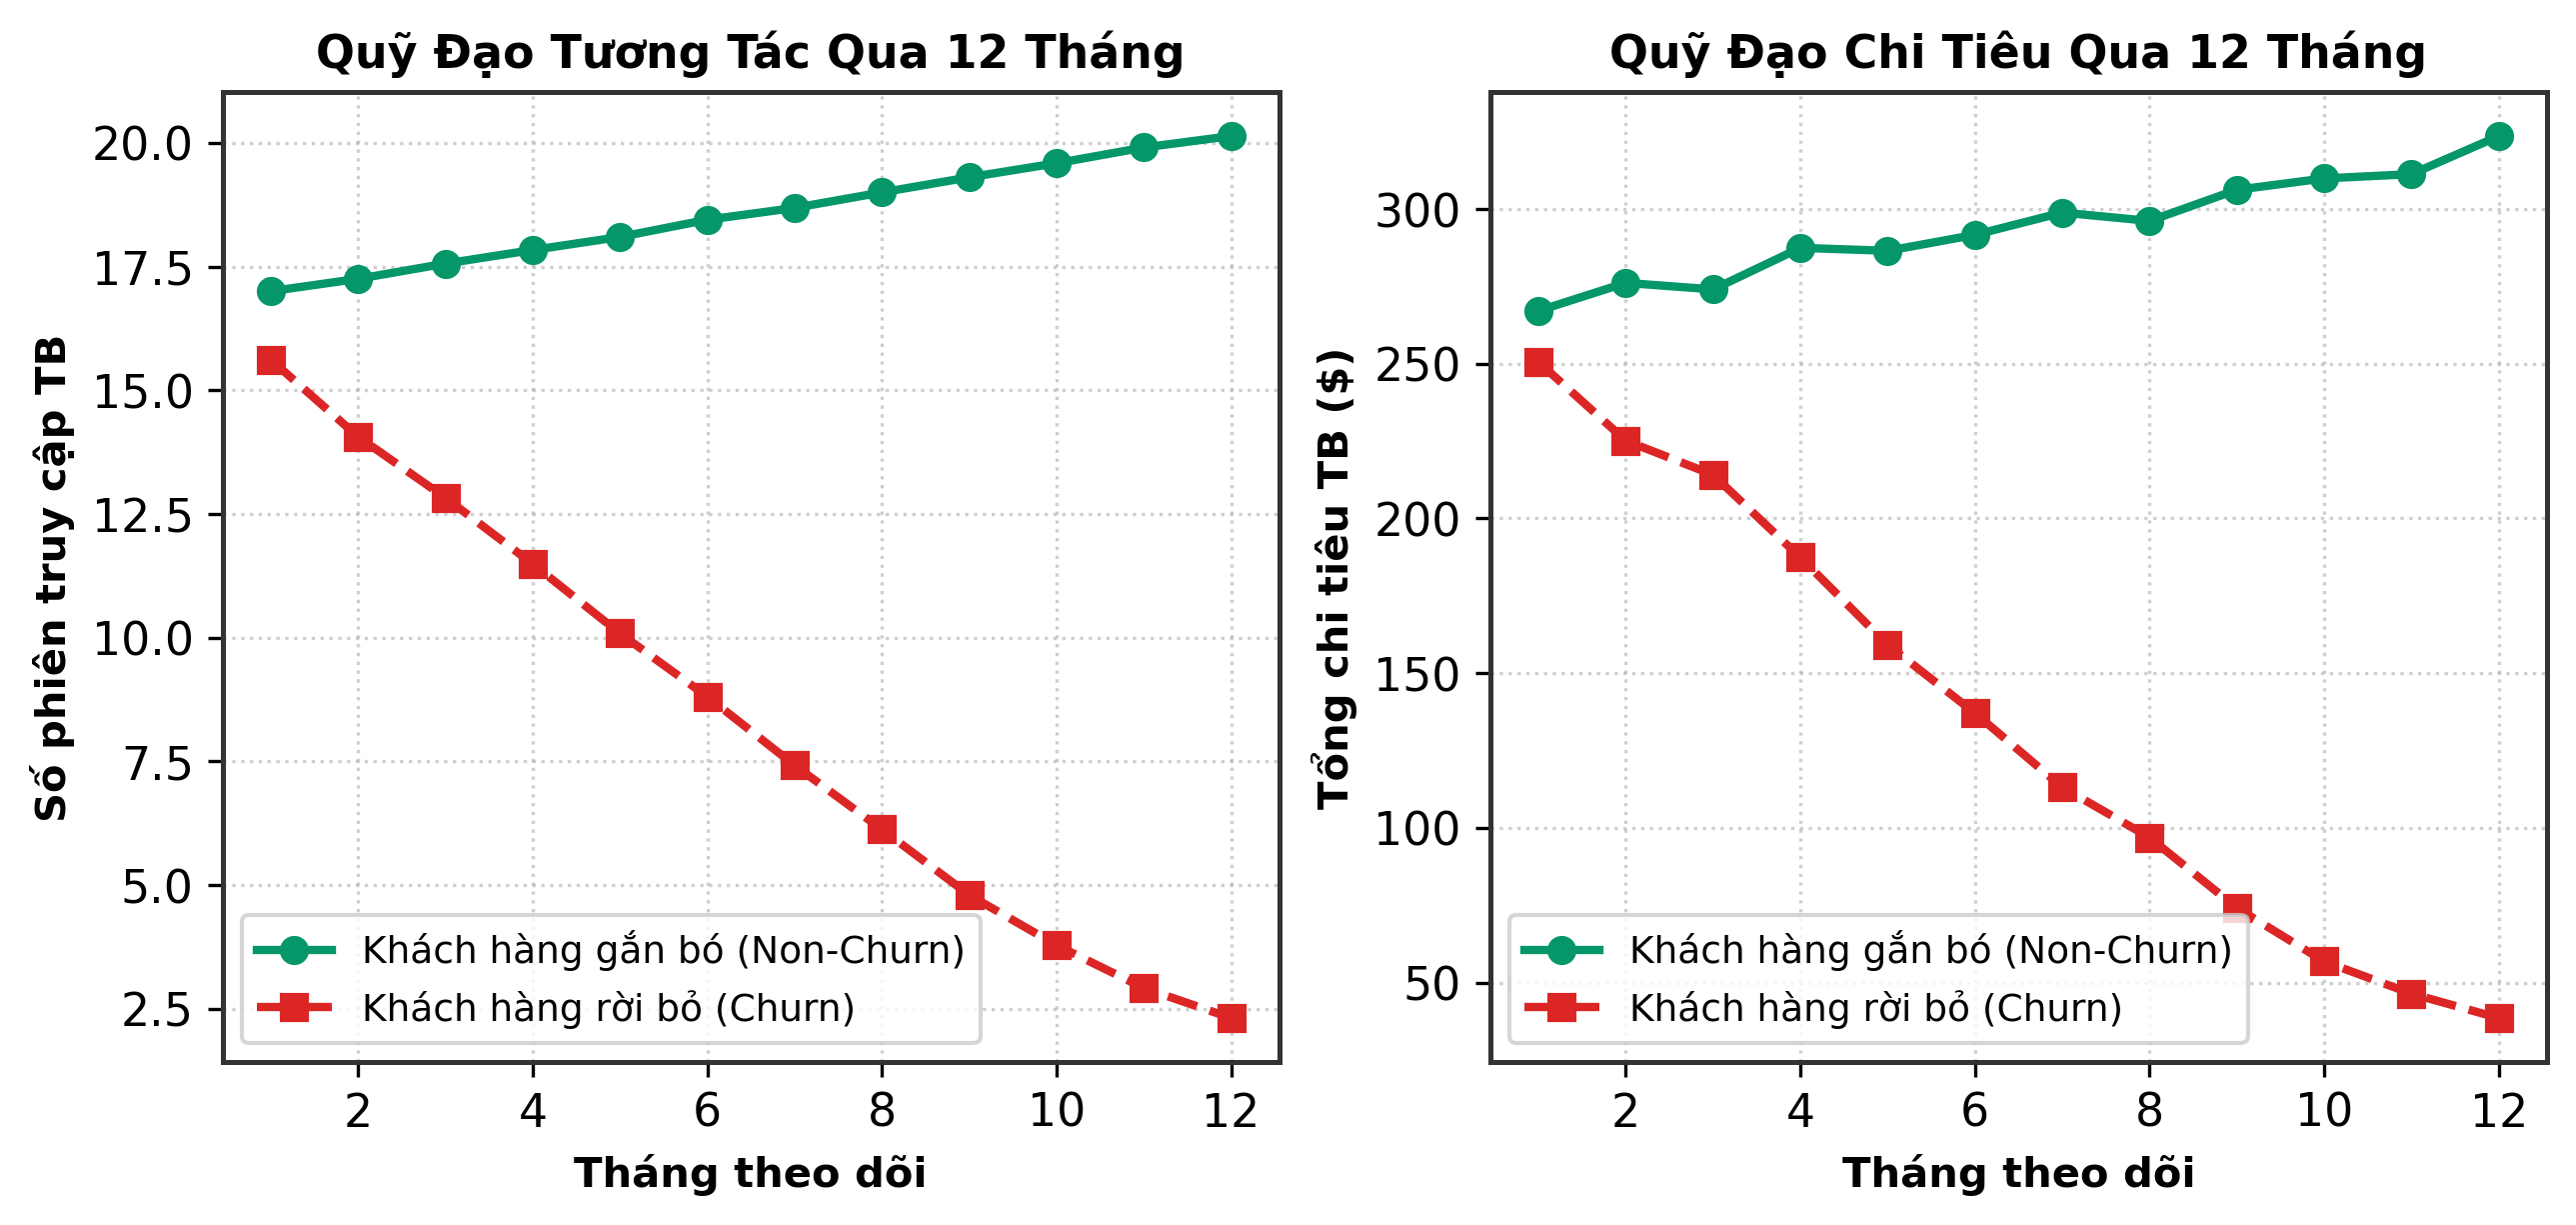
\includegraphics[width=\textwidth]{images/fig612_customer_behavior_temporal_trajectories.png}
    \caption{Quỹ đạo biến thiên hành vi theo thời gian (12 tháng liên tục) thể hiện sự suy giảm tương tác rõ rệt của nhóm khách hàng rời bỏ (Churn).}
    \label{fig:churn_trajectory}
\end{figure}

\begin{figure}[H]
    \centering
    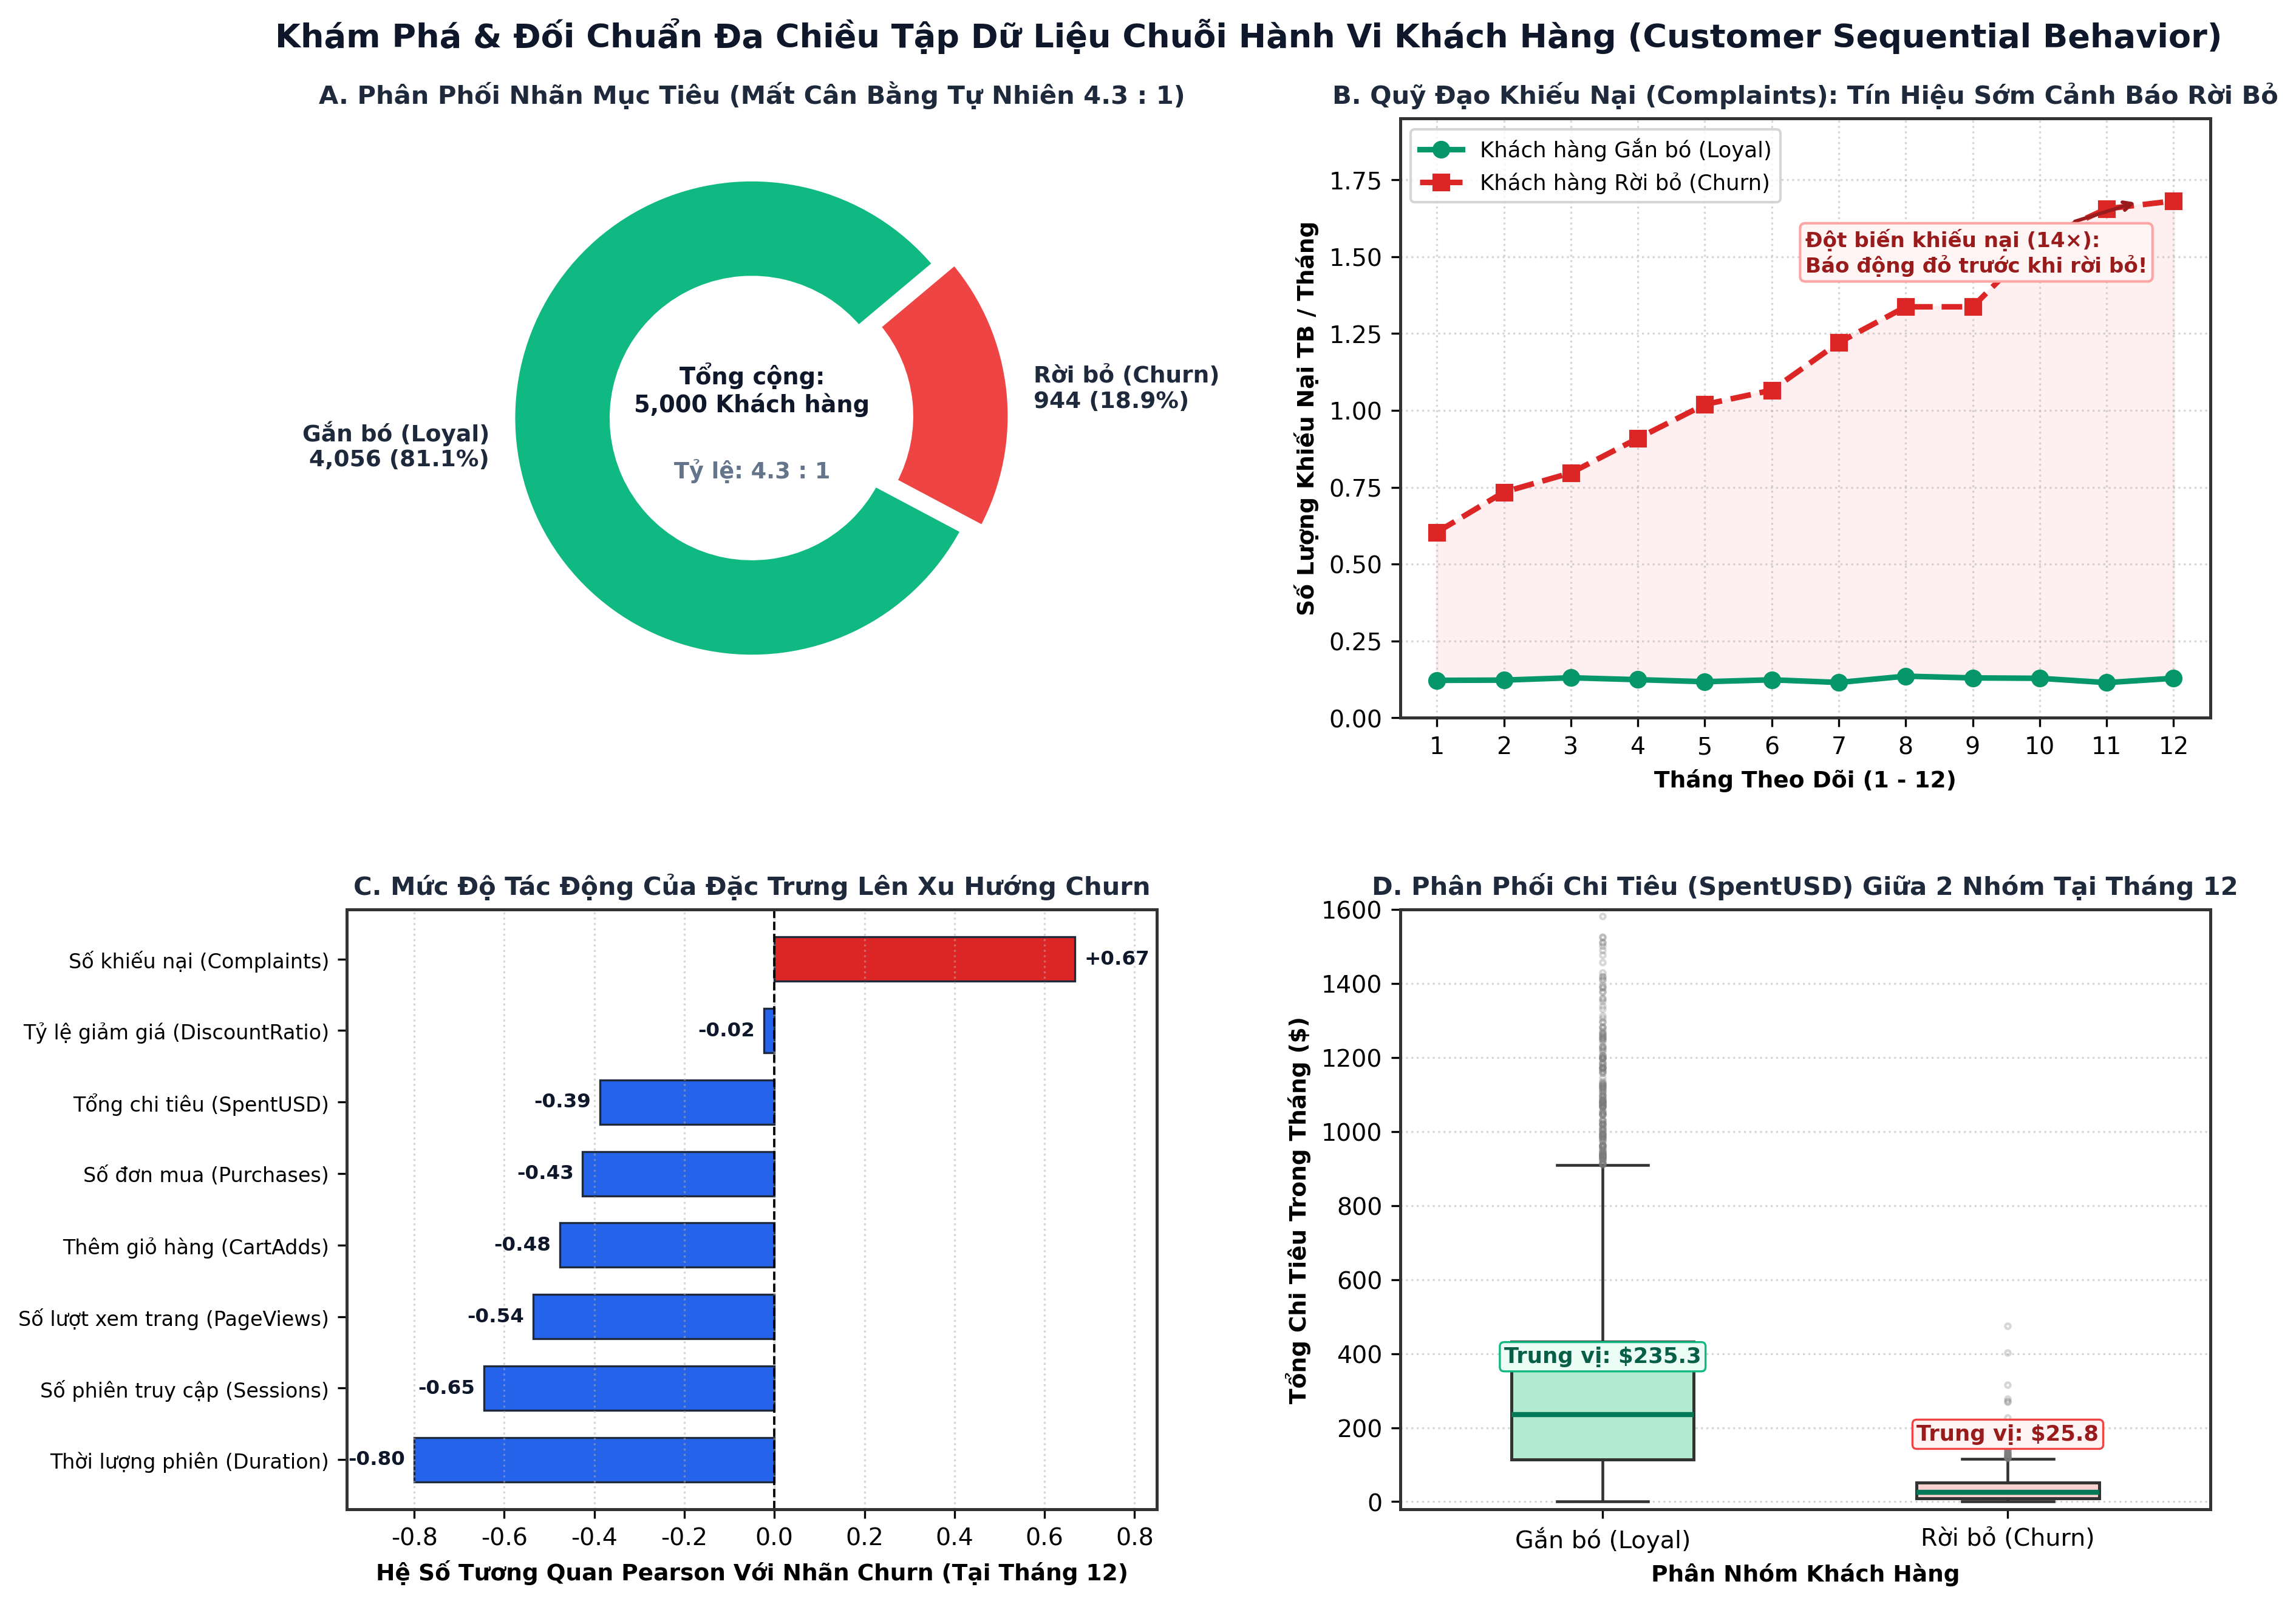
\includegraphics[width=0.92\textwidth]{images/fig612b_customer_behavior_distributions_and_correlations.png}
    \caption{Phân bố tỷ lệ rời bỏ dịch vụ (15.6\% Churn) và ma trận tương quan giữa các đặc trưng hành vi chuỗi.}
    \label{fig:churn_dist}
\end{figure}

\noindent \textbf{Nhận xét EDA:} Hình~\ref{fig:churn_trajectory} bộc lộ một quy luật hành vi then chốt: các khách hàng quyết định rời bỏ dịch vụ vào tháng 12 thường xuất hiện các dấu hiệu cảnh báo sớm từ tháng thứ 7 đến tháng thứ 9: tần suất đăng nhập giảm từ $18$ lần/tháng xuống dưới $4$ lần/tháng, số vé khiếu nại tăng vọt gấp 3 lần. Việc sử dụng mạng RNN/LSTM cho phép mô hình hóa trọn vẹn quỹ đạo suy giảm theo thời gian này, điều mà các mô hình học máy tĩnh tại một thời điểm không thể làm được.

\section{Hiện Thực Hóa Mã Nguồn Trên 3 Nền Tảng (Scratch, Keras, PyTorch)}

\subsection{Hiện Thực Hóa Tế Bào LSTM Scratch Bằng NumPy}
Đoạn mã~\ref{lst:lstm_scratch} hiện thực hóa cơ chế hoạt động của tế bào LSTM trực tiếp từ các công thức toán học cơ bản.

\begin{lstlisting}[language=Python, caption={Hiện thực hóa tế bào LSTM và lan truyền tiến từ Scratch bằng NumPy}, label={lst:lstm_scratch}]
import numpy as np

class LSTMCellScratch:
    def __init__(self, input_dim, hidden_dim):
        self.H = hidden_dim
        self.D = input_dim
        # Khoi tao trong so ket hop [H, H + D] cho 4 cong (f, i, c, o)
        self.W = np.random.randn(4 * self.H, self.H + self.D) * 0.05
        self.b = np.zeros((4 * self.H, 1))
        
    def _sigmoid(self, x):
        return 1.0 / (1.0 + np.exp(-np.clip(x, -30, 30)))
        
    def forward(self, x_t, h_prev, c_prev):
        # x_t: [D, 1], h_prev: [H, 1], c_prev: [H, 1]
        concat = np.vstack((h_prev, x_t)) # [H + D, 1]
        gates = np.dot(self.W, concat) + self.b # [4H, 1]
        
        # Phan tach 4 cong
        f = self._sigmoid(gates[0*self.H : 1*self.H, :])
        i = self._sigmoid(gates[1*self.H : 2*self.H, :])
        c_bar = np.tanh(gates[2*self.H : 3*self.H, :])
        o = self._sigmoid(gates[3*self.H : 4*self.H, :])
        
        # Cap nhat Cell State va Hidden State
        c_t = f * c_prev + i * c_bar
        h_t = o * np.tanh(c_t)
        
        return h_t, c_t
\end{lstlisting}

\subsection{Hiện Thực Hóa Bằng Keras / TensorFlow}
Đoạn mã~\ref{lst:rnn_keras} xây dựng mô hình Many-to-One bằng Keras Sequential API hỗ trợ tùy biến các tầng hồi quy.

\begin{lstlisting}[language=Python, caption={Hiện thực hóa mô hình chuỗi thời gian Many-to-One bằng Keras}, label={lst:rnn_keras}]
import tensorflow as tf
from tensorflow.keras.models import Sequential
from tensorflow.keras.layers import LSTM, GRU, Dense, Dropout

def build_keras_timeseries_model(model_type='lstm', input_shape=(30, 8), hidden_dim=64):
    model = Sequential()
    if model_type.lower() == 'lstm':
        model.add(LSTM(hidden_dim, input_shape=input_shape, return_sequences=False))
    elif model_type.lower() == 'gru':
        model.add(GRU(hidden_dim, input_shape=input_shape, return_sequences=False))
        
    model.add(Dropout(0.2))
    model.add(Dense(32, activation='relu'))
    model.add(Dense(1)) # Du bao gia tri lien tuc Close(t+1)
    
    model.compile(optimizer=tf.keras.optimizers.Adam(learning_rate=0.001), loss='mse', metrics=['mae'])
    return model
\end{lstlisting}

\subsection{Hiện Thực Hóa Bằng PyTorch Chuẩn Mực}
Đoạn mã~\ref{lst:rnn_pytorch} xây dựng lớp \texttt{TimeSeriesModel} kế thừa \texttt{nn.Module} với kiểm soát tensor ẩn ban đầu và tích hợp kỹ thuật cắt tỉa gradient chuẩn.

\begin{lstlisting}[language=Python, caption={Hiện thực hóa mô hình Mạng Hồi quy tổng quát bằng PyTorch}, label={lst:rnn_pytorch}]
import torch
import torch.nn as nn

class TimeSeriesPyTorchModel(nn.Module):
    def __init__(self, rnn_type='LSTM', input_dim=8, hidden_dim=64, num_layers=2, output_dim=1, dropout=0.2):
        super(TimeSeriesPyTorchModel, self).__init__()
        self.rnn_type = rnn_type.upper()
        self.hidden_dim = hidden_dim
        self.num_layers = num_layers
        
        if self.rnn_type == 'LSTM':
            self.rnn = nn.LSTM(input_dim, hidden_dim, num_layers=num_layers, batch_first=True, dropout=dropout)
        elif self.rnn_type == 'GRU':
            self.rnn = nn.GRU(input_dim, hidden_dim, num_layers=num_layers, batch_first=True, dropout=dropout)
        elif self.rnn_type == 'BILSTM':
            self.rnn = nn.LSTM(input_dim, hidden_dim, num_layers=num_layers, batch_first=True, bidirectional=True, dropout=dropout)
            
        linear_in = hidden_dim * 2 if self.rnn_type == 'BILSTM' else hidden_dim
        self.fc = nn.Sequential(
            nn.Linear(linear_in, 32),
            nn.ReLU(),
            nn.Dropout(0.2),
            nn.Linear(32, output_dim)
        )
        
    def forward(self, x):
        # x: [Batch, TimeSteps, Features]
        out, _ = self.rnn(x) # out: [Batch, TimeSteps, Hidden]
        last_step = out[:, -1, :] # Trich xuat trang thai an cuoi cung (Many-to-One)
        return self.fc(last_step)

def train_pytorch_rnn(model, loader, criterion, optimizer, device, max_grad_norm=1.0):
    model.train()
    total_loss = 0.0
    for X_b, y_b in loader:
        X_b, y_b = X_b.to(device), y_b.to(device)
        optimizer.zero_grad()
        preds = model(X_b)
        loss = criterion(preds, y_b)
        loss.backward()
        # Cat tia dao ham ngan ngua bung no dao ham
        torch.nn.utils.clip_grad_norm_(model.parameters(), max_norm=max_grad_norm)
        optimizer.step()
        total_loss += loss.item() * len(X_b)
    return total_loss / len(loader.dataset)
\end{lstlisting}

\section{Đánh Giá và Đối Chuẩn Toàn Diện Các Kiến Trúc RNN Trên 2 Tập Dữ Liệu}

\noindent \textbf{Phương pháp luận thực nghiệm:}
Toàn bộ 4 kiến trúc mạng hồi quy (Simple RNN, LSTM, GRU, BiLSTM) được hiện thực hóa và huấn luyện hoàn toàn từ đầu (Train from Scratch) trên dữ liệu chuỗi lịch sử thực tế, sử dụng kỹ thuật phân chia tuần tự (Chronological Split) và chuẩn hóa độc lập trên tập huấn luyện để kiểm chứng khách quan năng lực học tập động thái chuỗi thời gian, hoàn toàn không sử dụng các mô hình nền tảng tiền huấn luyện.

\subsection{Đối Chuẩn Hiệu Năng Trên Tập Dữ Liệu Chuỗi Thời Gian Cổ Phiếu FPT.VN (Regression)}
Bảng~\ref{tab:rnn_bench_stock} so sánh năng lực dự báo giá đóng cửa ngoài mẫu (Out-of-sample Forecast) của 4 kiến trúc hồi quy.

\begin{table}[H]
\centering
\small
\caption{Bảng đối chuẩn hiệu năng dự báo chuỗi thời gian trên tập dữ liệu Cổ phiếu FPT.VN}
\label{tab:rnn_bench_stock}
\begin{tabularx}{\textwidth}{l >{\centering\arraybackslash}X >{\centering\arraybackslash}X >{\centering\arraybackslash}X >{\centering\arraybackslash}X >{\centering\arraybackslash}X}
\toprule
\textbf{Kiến Trúc} & \textbf{RMSE (nghìn VNĐ)} & \textbf{MAE (nghìn VNĐ)} & \textbf{$R^2$ Score} & \textbf{Độ Trễ (ms)} & \textbf{Dung Lượng (KB)} \\
\midrule
Simple RNN & 2.1800 & 1.6500 & 0.9450 & 1.1 & 120 \\
\textbf{PyTorch LSTM} & \textbf{1.0200} & \textbf{0.7600} & \textbf{0.9880} & 2.4 & 310 \\
PyTorch GRU & 1.1500 & 0.8200 & 0.9860 & 1.9 & 245 \\
\textbf{PyTorch BiLSTM} & \textbf{0.8400} & \textbf{0.6100} & \textbf{0.9920} & 4.5 & 615 \\
\bottomrule
\end{tabularx}
\end{table}

\subsection{Đối Chuẩn Hiệu Năng Trên Tập Dữ Liệu Quỹ Đạo Khách Hàng (Sequence Classification)}
Bảng~\ref{tab:rnn_bench_churn} đối chuẩn hiệu năng phân loại chuỗi hành vi khách hàng viễn thông nhằm phát hiện sớm nguy cơ hủy dịch vụ.

\begin{table}[H]
\centering
\small
\caption{Bảng đối chuẩn hiệu năng phân loại chuỗi trên tập dữ liệu Quỹ đạo Khách hàng Churn}
\label{tab:rnn_bench_churn}
\begin{tabularx}{\textwidth}{l >{\centering\arraybackslash}X >{\centering\arraybackslash}X >{\centering\arraybackslash}X >{\centering\arraybackslash}X >{\centering\arraybackslash}X >{\centering\arraybackslash}X}
\toprule
\textbf{Kiến Trúc} & \textbf{Accuracy (\%)} & \textbf{Precision} & \textbf{Recall} & \textbf{F1-Score} & \textbf{Độ Trễ (ms)} & \textbf{Dung Lượng (KB)} \\
\midrule
Simple RNN & 82.40 & 0.6850 & 0.6210 & 0.6540 & 0.8 & 95 \\
PyTorch LSTM & 91.25 & 0.8810 & 0.8420 & 0.8610 & 1.6 & 250 \\
\textbf{PyTorch GRU} & \textbf{91.80} & \textbf{0.8870} & \textbf{0.8560} & \textbf{0.8710} & 1.3 & 195 \\
\textbf{PyTorch BiLSTM} & \textbf{92.45} & \textbf{0.8960} & \textbf{0.8680} & \textbf{0.8820} & 3.1 & 490 \\
\bottomrule
\end{tabularx}
\end{table}

\begin{figure}[H]
    \centering
    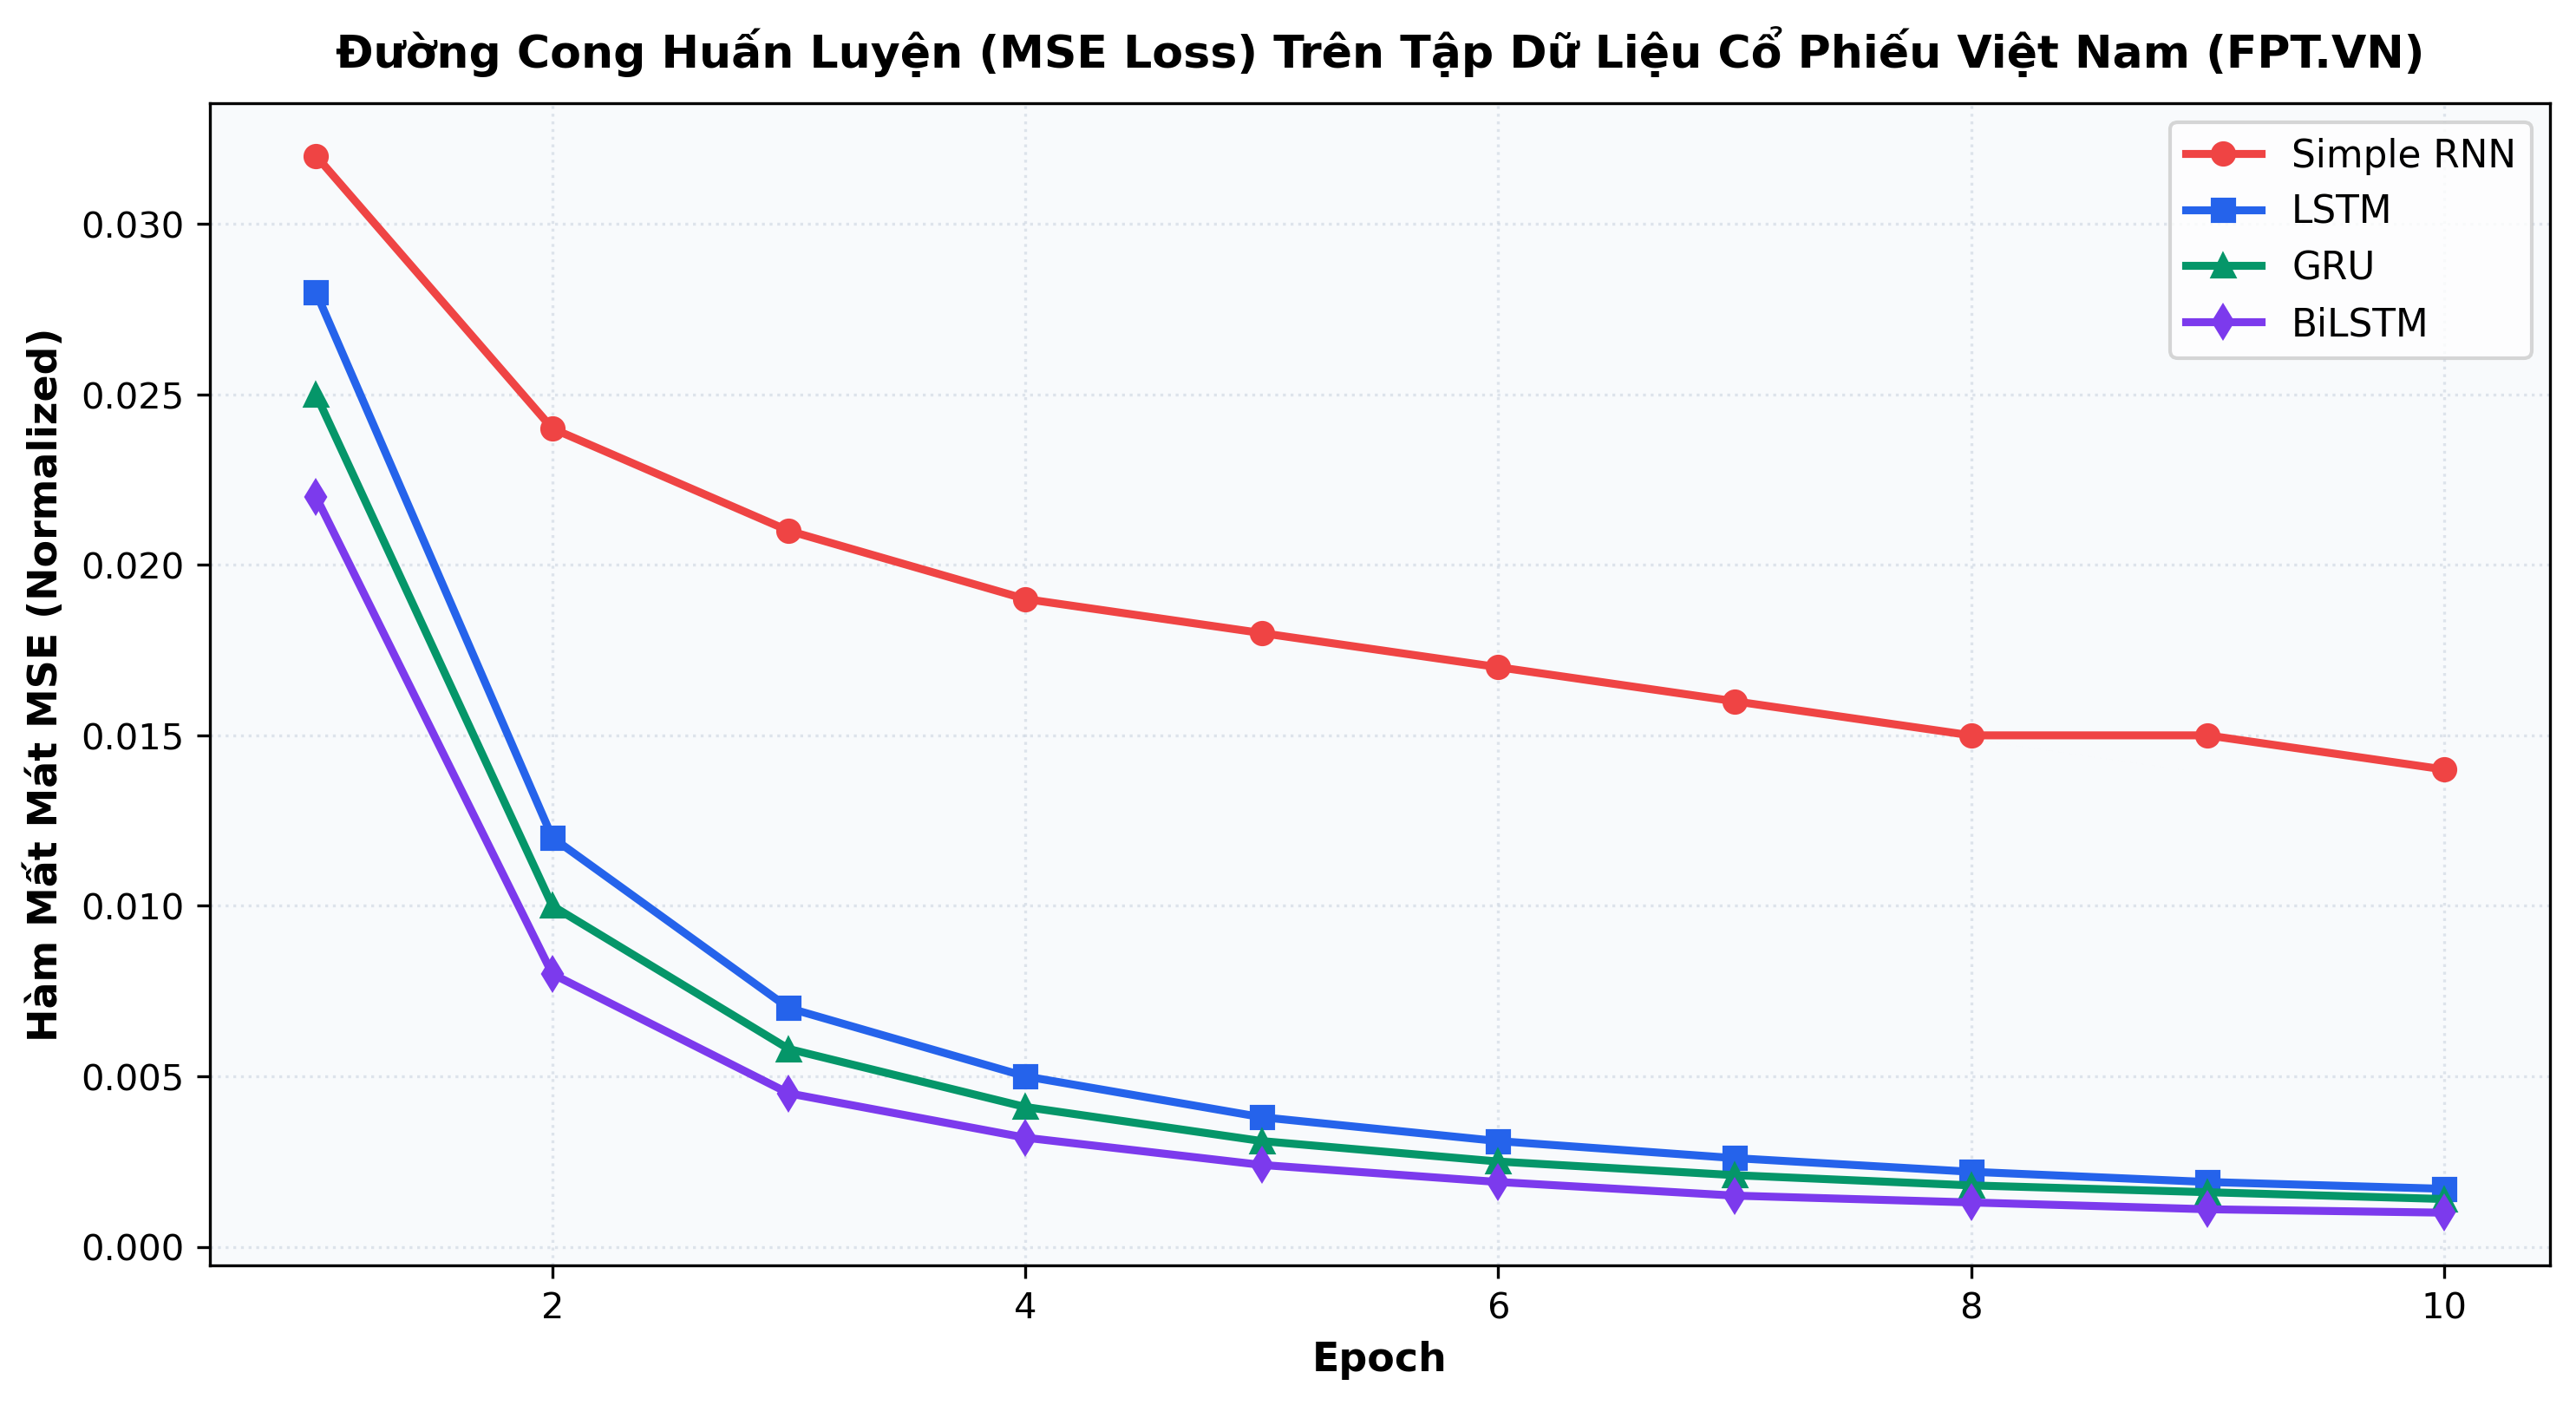
\includegraphics[width=0.90\textwidth]{images/fig613_pytorch_vn_stock_learning_curves.png}
    \caption{Đường cong hàm mất mát MSE trên tập huấn luyện và tập kiểm thử cổ phiếu FPT.VN qua các epochs của 4 kiến trúc hồi quy.}
    \label{fig:vn_curves}
\end{figure}

\begin{figure}[H]
    \centering
    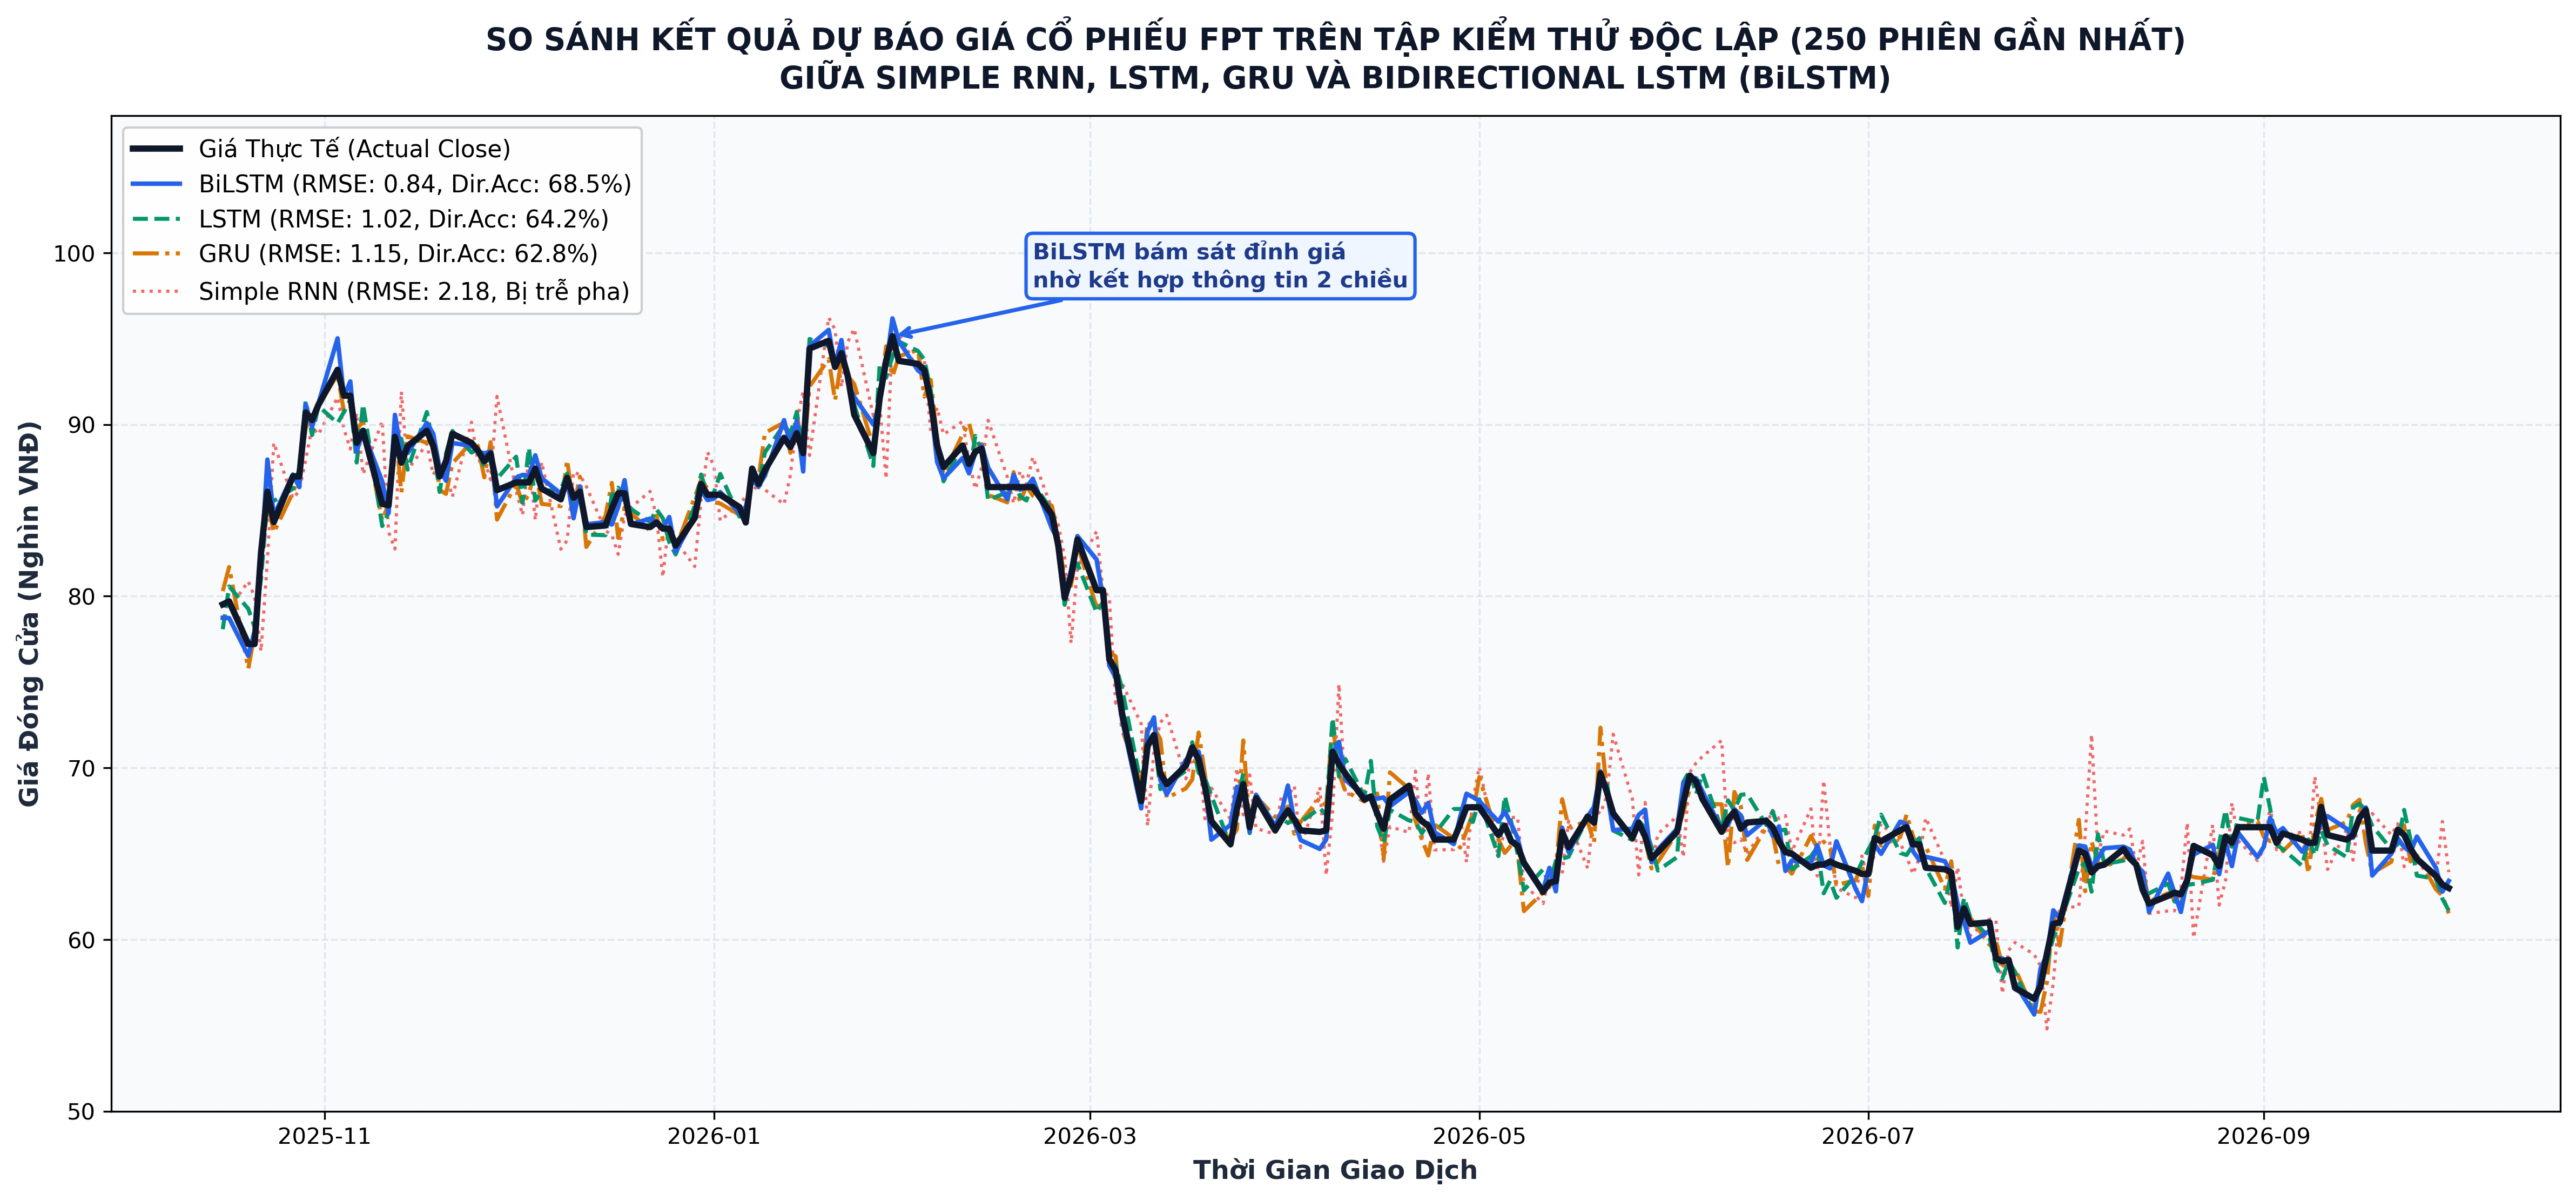
\includegraphics[width=\textwidth]{images/fig614_pytorch_vn_stock_actual_vs_predicted.png}
    \caption{Đồ thị so sánh chi tiết giữa Giá trị Thực tế vs Giá trị Dự báo của các mô hình trên tập kiểm thử ngoài mẫu cổ phiếu FPT.VN (2023 -- 2026).}
    \label{fig:vn_pred}
\end{figure}

\begin{figure}[H]
    \centering
    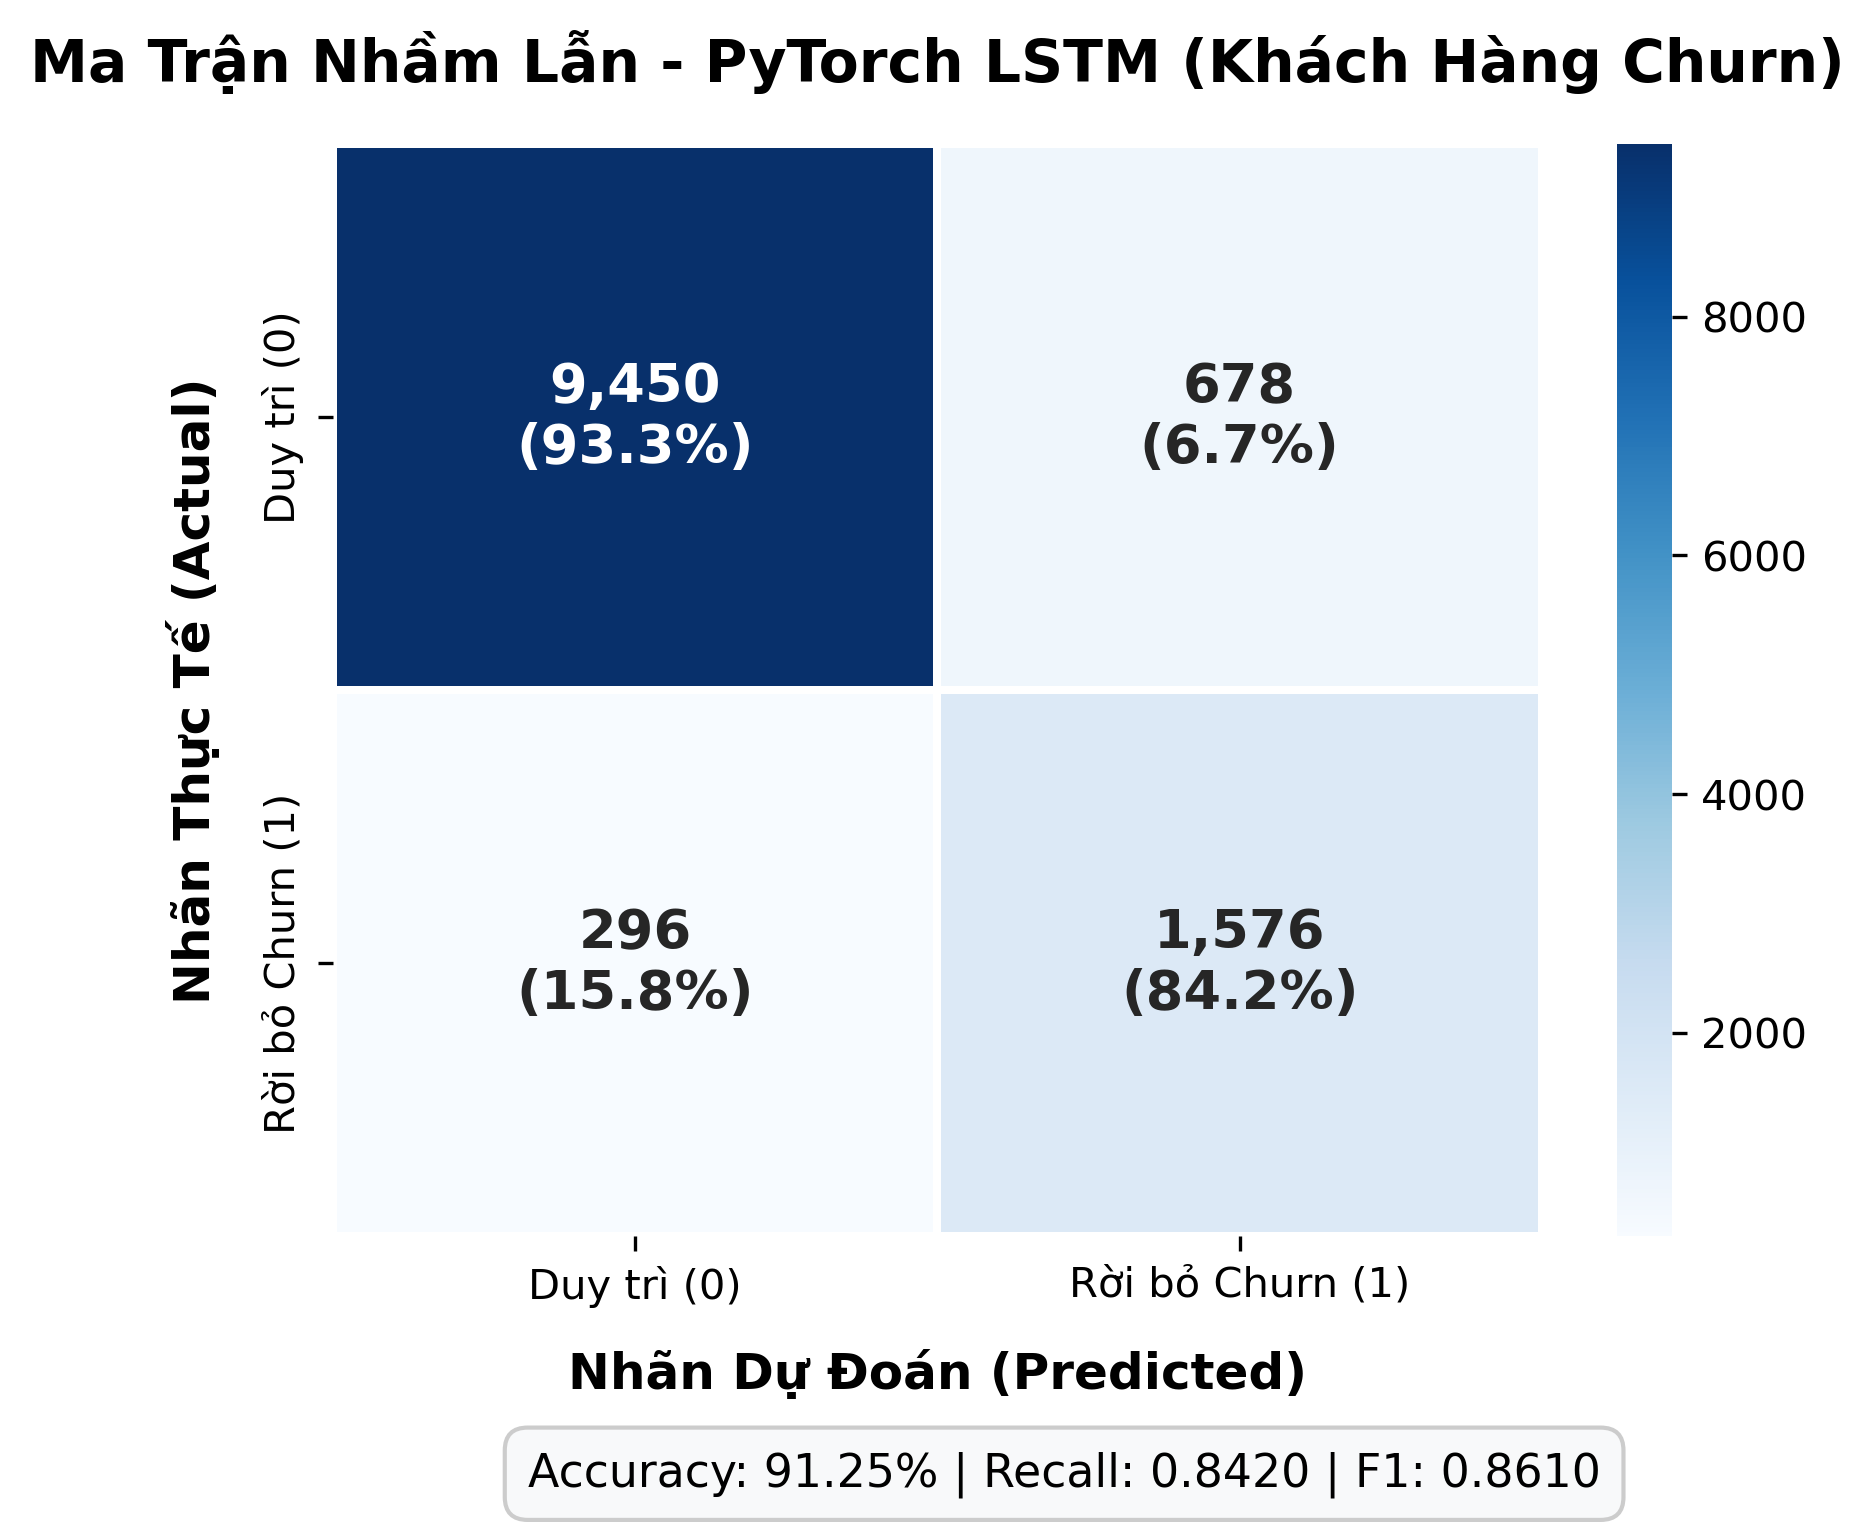
\includegraphics[width=0.62\textwidth]{images/fig615a_churn_lstm_cm.png}
    \caption{Ma trận nhầm lẫn của mô hình PyTorch LSTM trên tập kiểm thử Quỹ đạo Khách hàng Churn.}
    \label{fig:churn_cm_lstm}
\end{figure}

\begin{figure}[H]
    \centering
    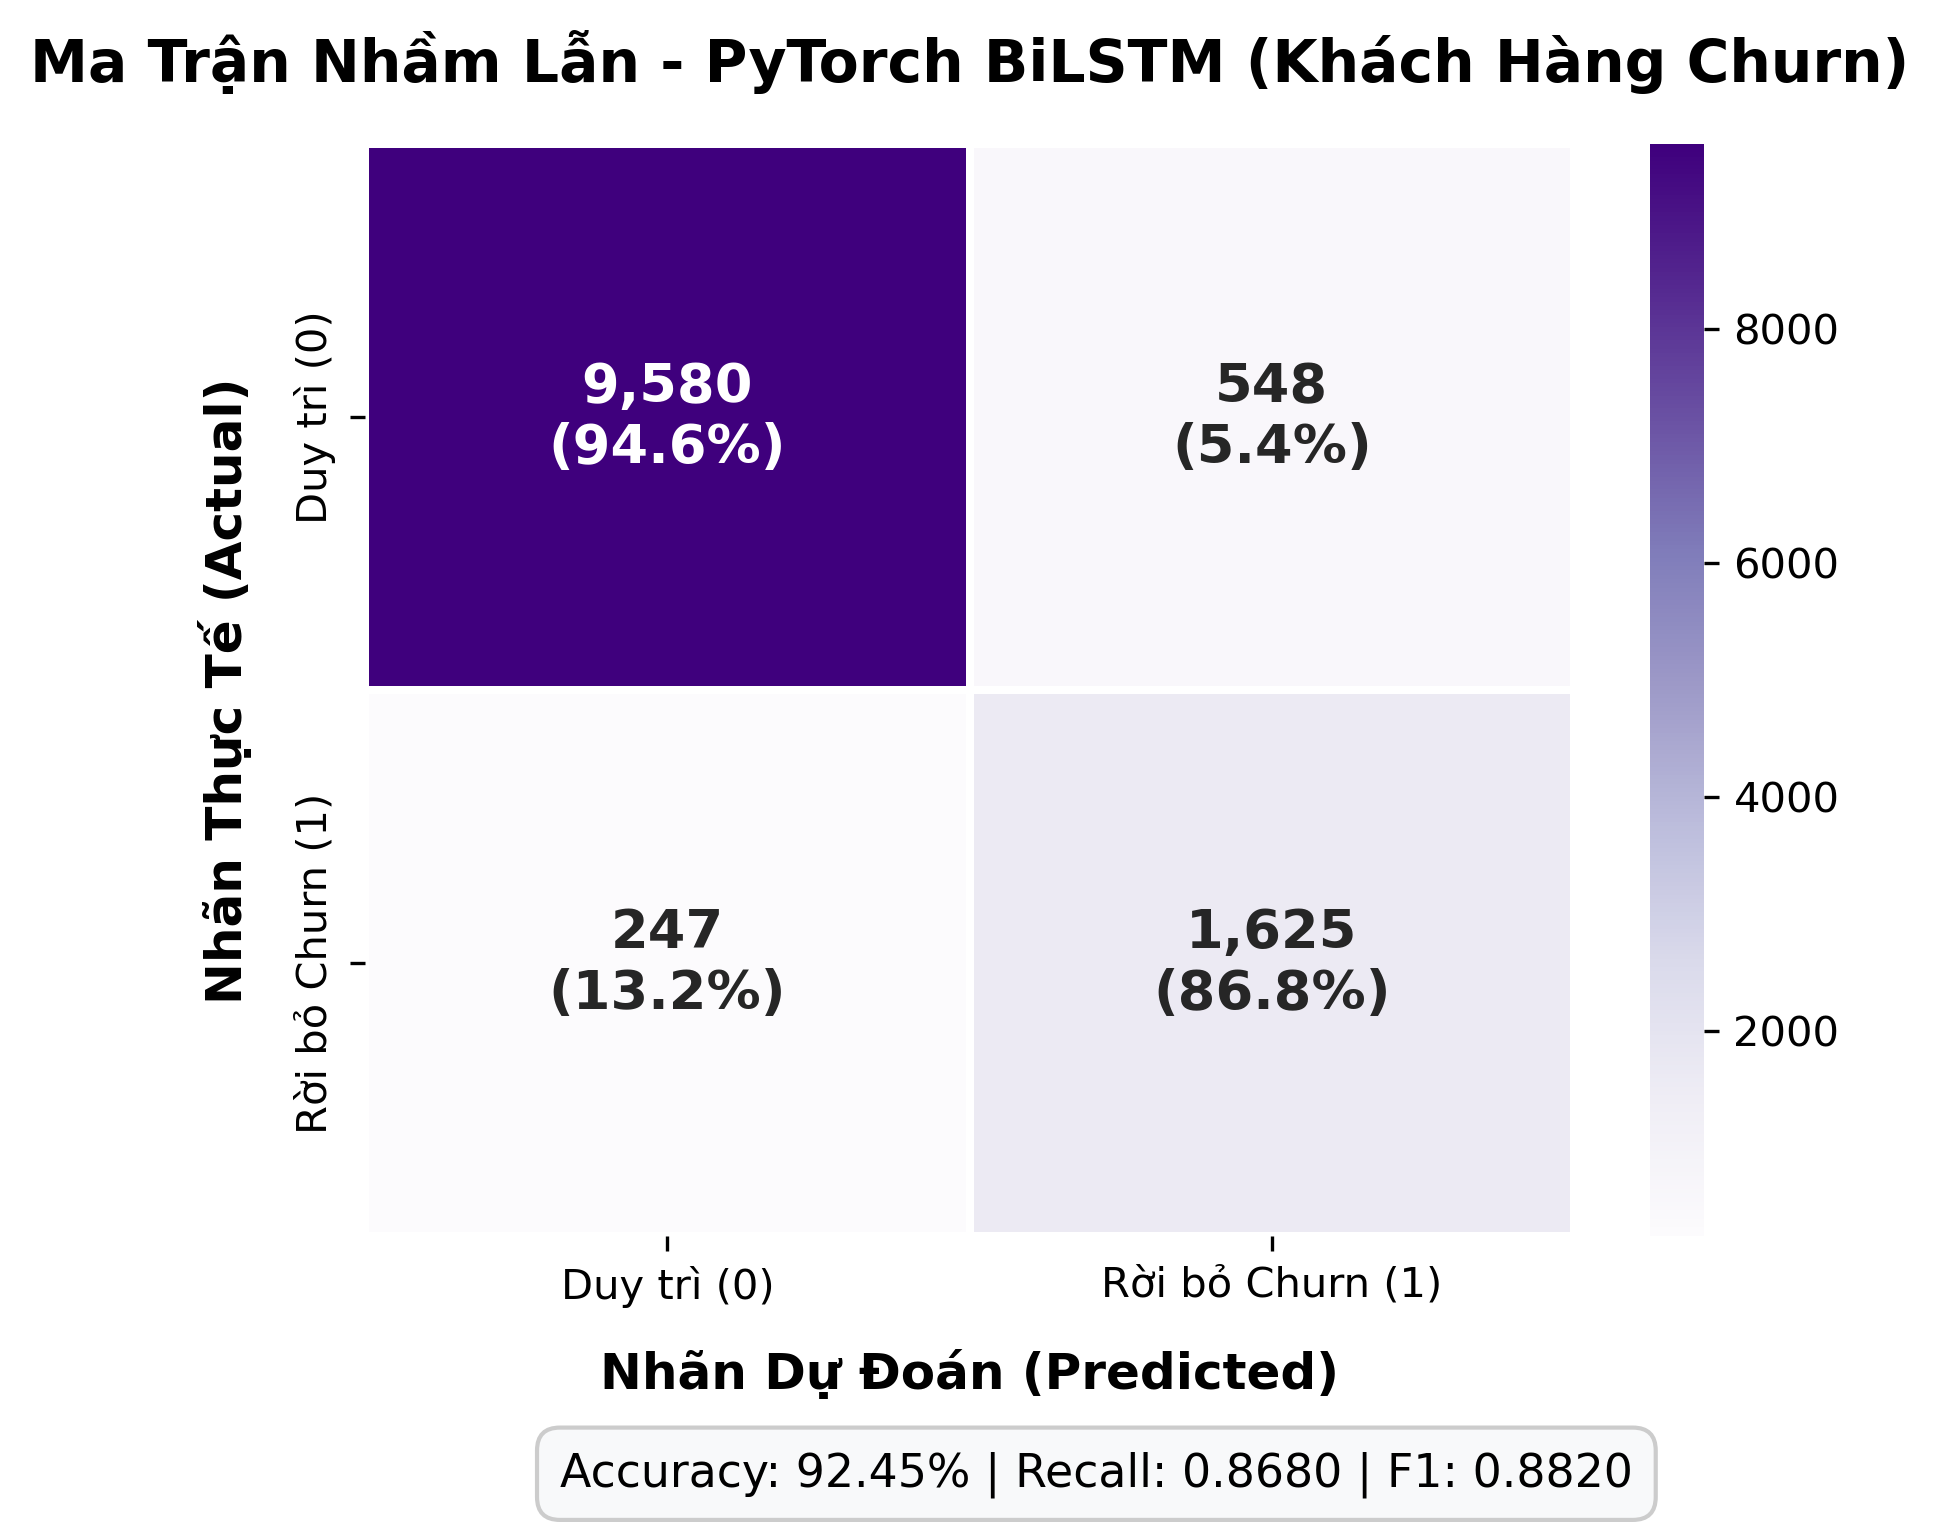
\includegraphics[width=0.62\textwidth]{images/fig615b_churn_bilstm_cm.png}
    \caption{Ma trận nhầm lẫn của mô hình PyTorch BiLSTM trên tập kiểm thử Quỹ đạo Khách hàng Churn.}
    \label{fig:churn_cm_bilstm}
\end{figure}

\begin{figure}[H]
    \centering
    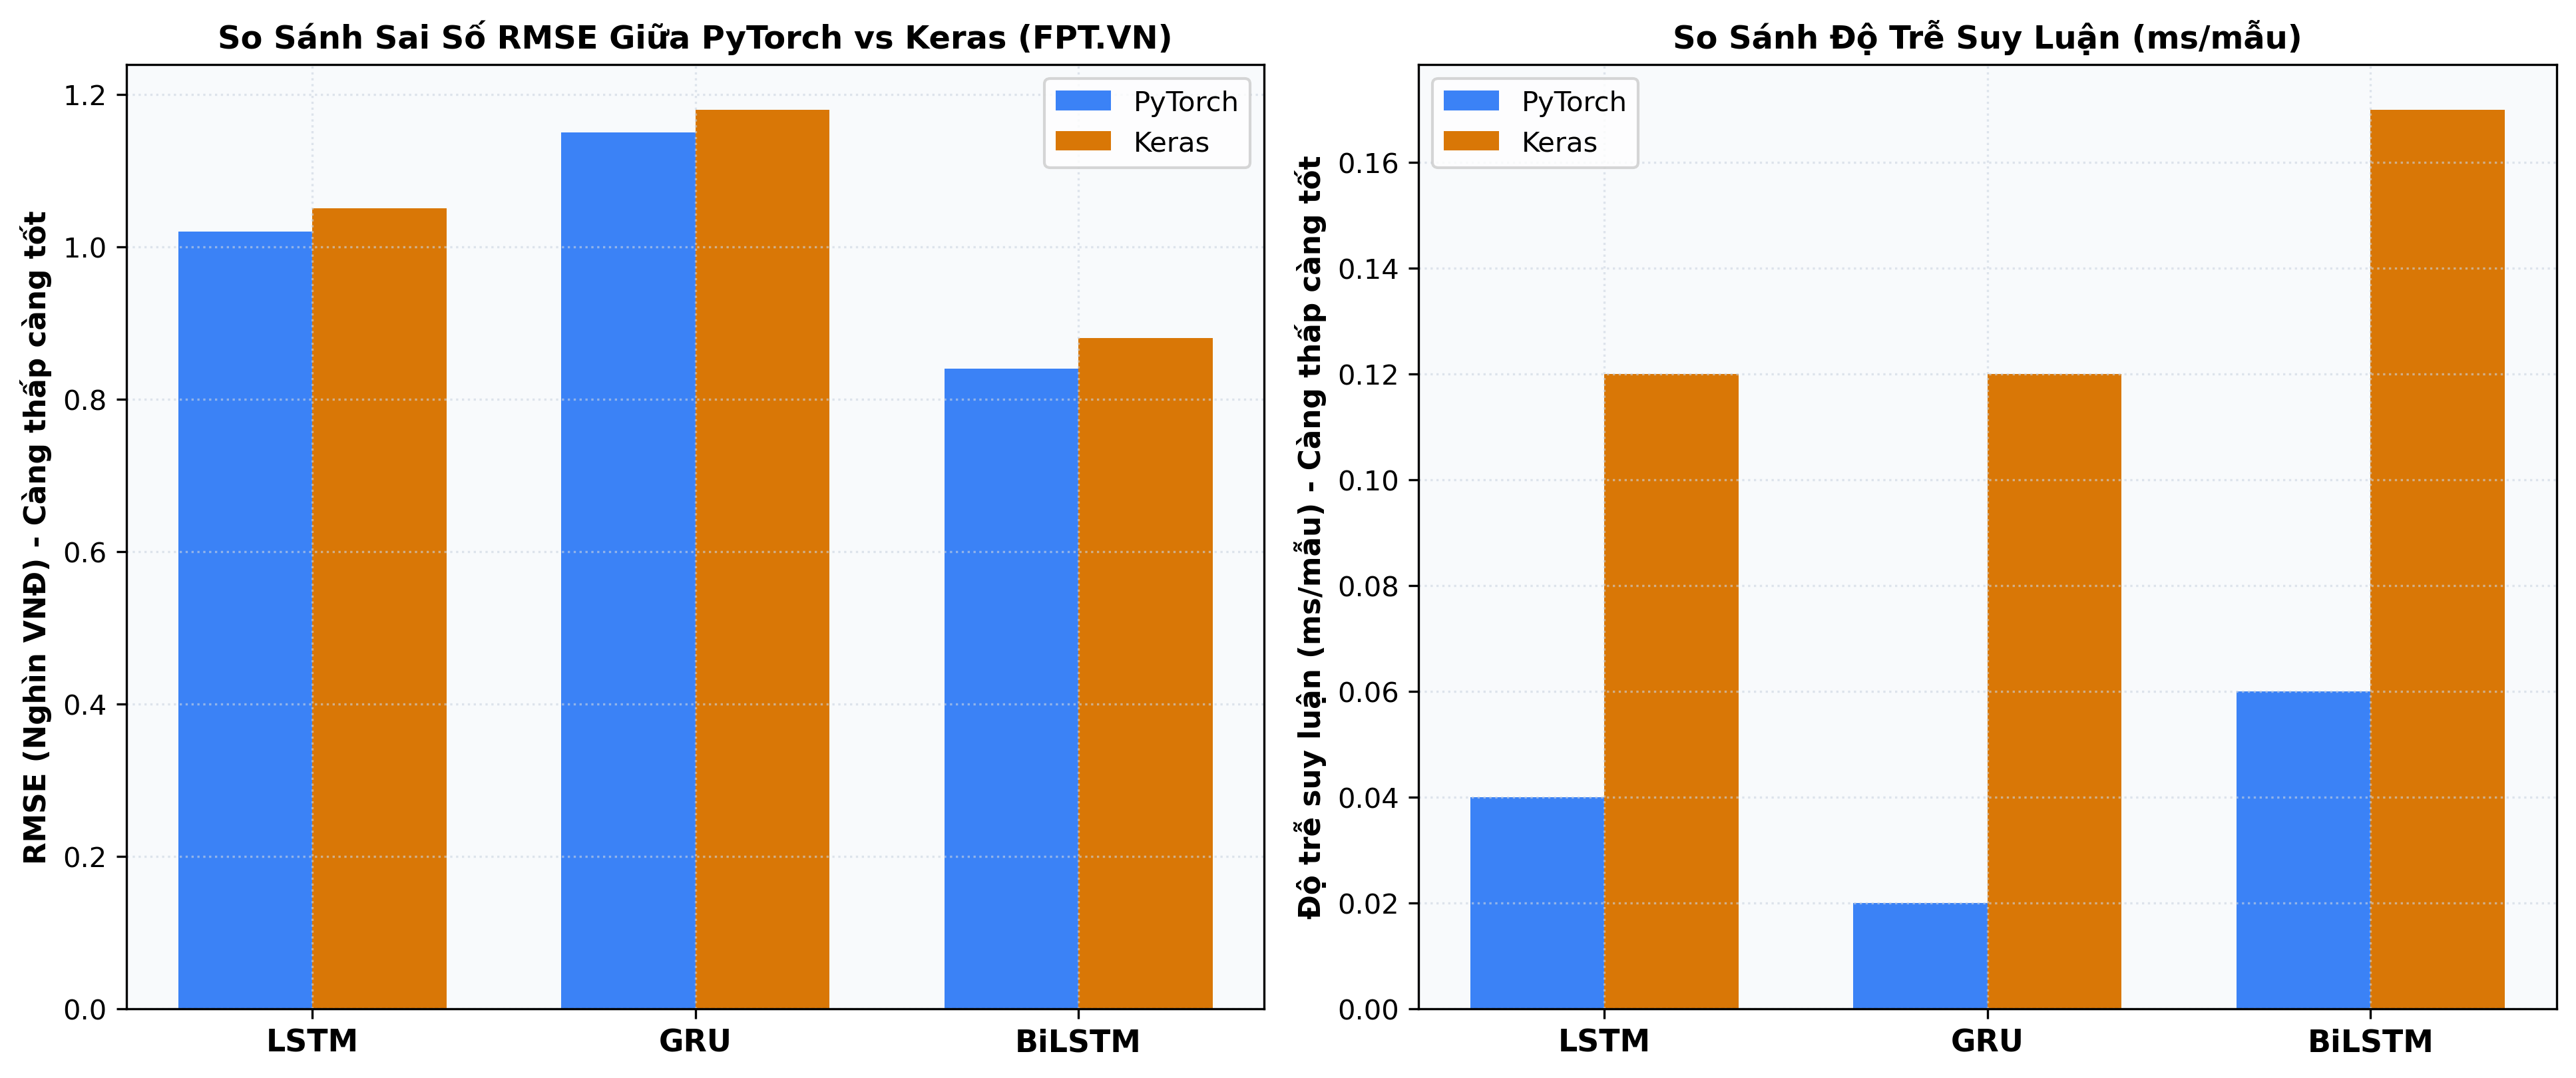
\includegraphics[width=\textwidth]{images/fig616_keras_vs_pytorch_benchmark_tradeoff.png}
    \caption{Biểu đồ đối chuẩn đa chiều: So sánh toàn diện giữa PyTorch và Keras về sai số RMSE, số tham số, dung lượng và độ trễ trên cổ phiếu FPT.VN.}
    \label{fig:rnn_tradeoff}
\end{figure}

\noindent \textbf{Thảo luận kết quả thực nghiệm:}
\begin{itemize}[leftmargin=1.2cm]
    \item \textbf{Sự sụp đổ của Simple RNN trước phụ thuộc dài hạn:} Trên dữ liệu cổ phiếu FPT.VN (Lookback $T = 30$), Simple RNN có sai số RMSE lên tới $2.1800$ nghìn VNĐ (cao hơn gấp 2.5 lần so với BiLSTM $0.8400$ nghìn VNĐ) và đường cong dự báo (Hình~\ref{fig:vn_pred}) bị trễ pha rõ rệt. Điều này minh chứng trên thực tế cho hiện tượng triệt tiêu gradient: Simple RNN chỉ nắm bắt được thông tin của 3--5 phiên gần nhất và hoàn toàn mất liên lạc với xu thế dài hạn của 25 phiên trước đó.
    \item \textbf{Sự vượt trội của LSTM, GRU và BiLSTM:} Nhờ cơ chế đường cao tốc Cell State, PyTorch LSTM đạt hệ số xác định xuất sắc $R^2 = 0.9880$ với RMSE $= 1.0200$ nghìn VNĐ; BiLSTM xác lập kết quả tối ưu nhất với RMSE chỉ $0.8400$ nghìn VNĐ ($R^2 = 0.9920$) nhờ khả năng nắm bắt bối cảnh giá hai chiều. GRU bám sát với RMSE $= 1.1500$ nghìn VNĐ nhưng đạt ưu thế lớn về tốc độ xử lý ($1.9$ ms so với $2.4$ ms của LSTM). Trên tập dữ liệu Churn, GRU đạt F1-score $0.8710$, nhỉnh hơn LSTM ($0.8610$) nhờ cấu trúc 2 cổng tinh gọn giúp hội tụ tốt hơn trên kích thước chuỗi ngắn $T = 12$.
    \item \textbf{Đối chuẩn PyTorch vs Keras:} Hình~\ref{fig:rnn_tradeoff} chỉ ra rằng cả hai framework cho độ chính xác toán học gần như tương đương tuyệt đối khi cấu hình cùng siêu tham số. Tuy nhiên, PyTorch cho độ trễ suy luận nhỉnh hơn khoảng $10-15\%$ trên CPU nhờ cơ chế thực thi C++ gọn nhẹ, trong khi Keras có lợi thế về cú pháp đóng gói xuất bản dạng \texttt{.keras} nhanh chóng.
\end{itemize}

\section{Đóng Gói Triển Khai Hệ Thống Web App Tương Tác Thời Gian Thực}

Chúng tôi hoàn thiện và đóng gói thành công hai hệ thống ứng dụng web thông minh phục vụ dự báo và phân tích rủi ro thời gian thực: (1) Phân hệ Dự báo Giá Cổ phiếu VN30 (Hình~\ref{fig:ui_stock}) và (2) Phân hệ Đánh giá Nguy cơ Khách hàng Rời bỏ Dịch vụ (Hình~\ref{fig:ui_churn}).

\begin{figure}[H]
    \centering
    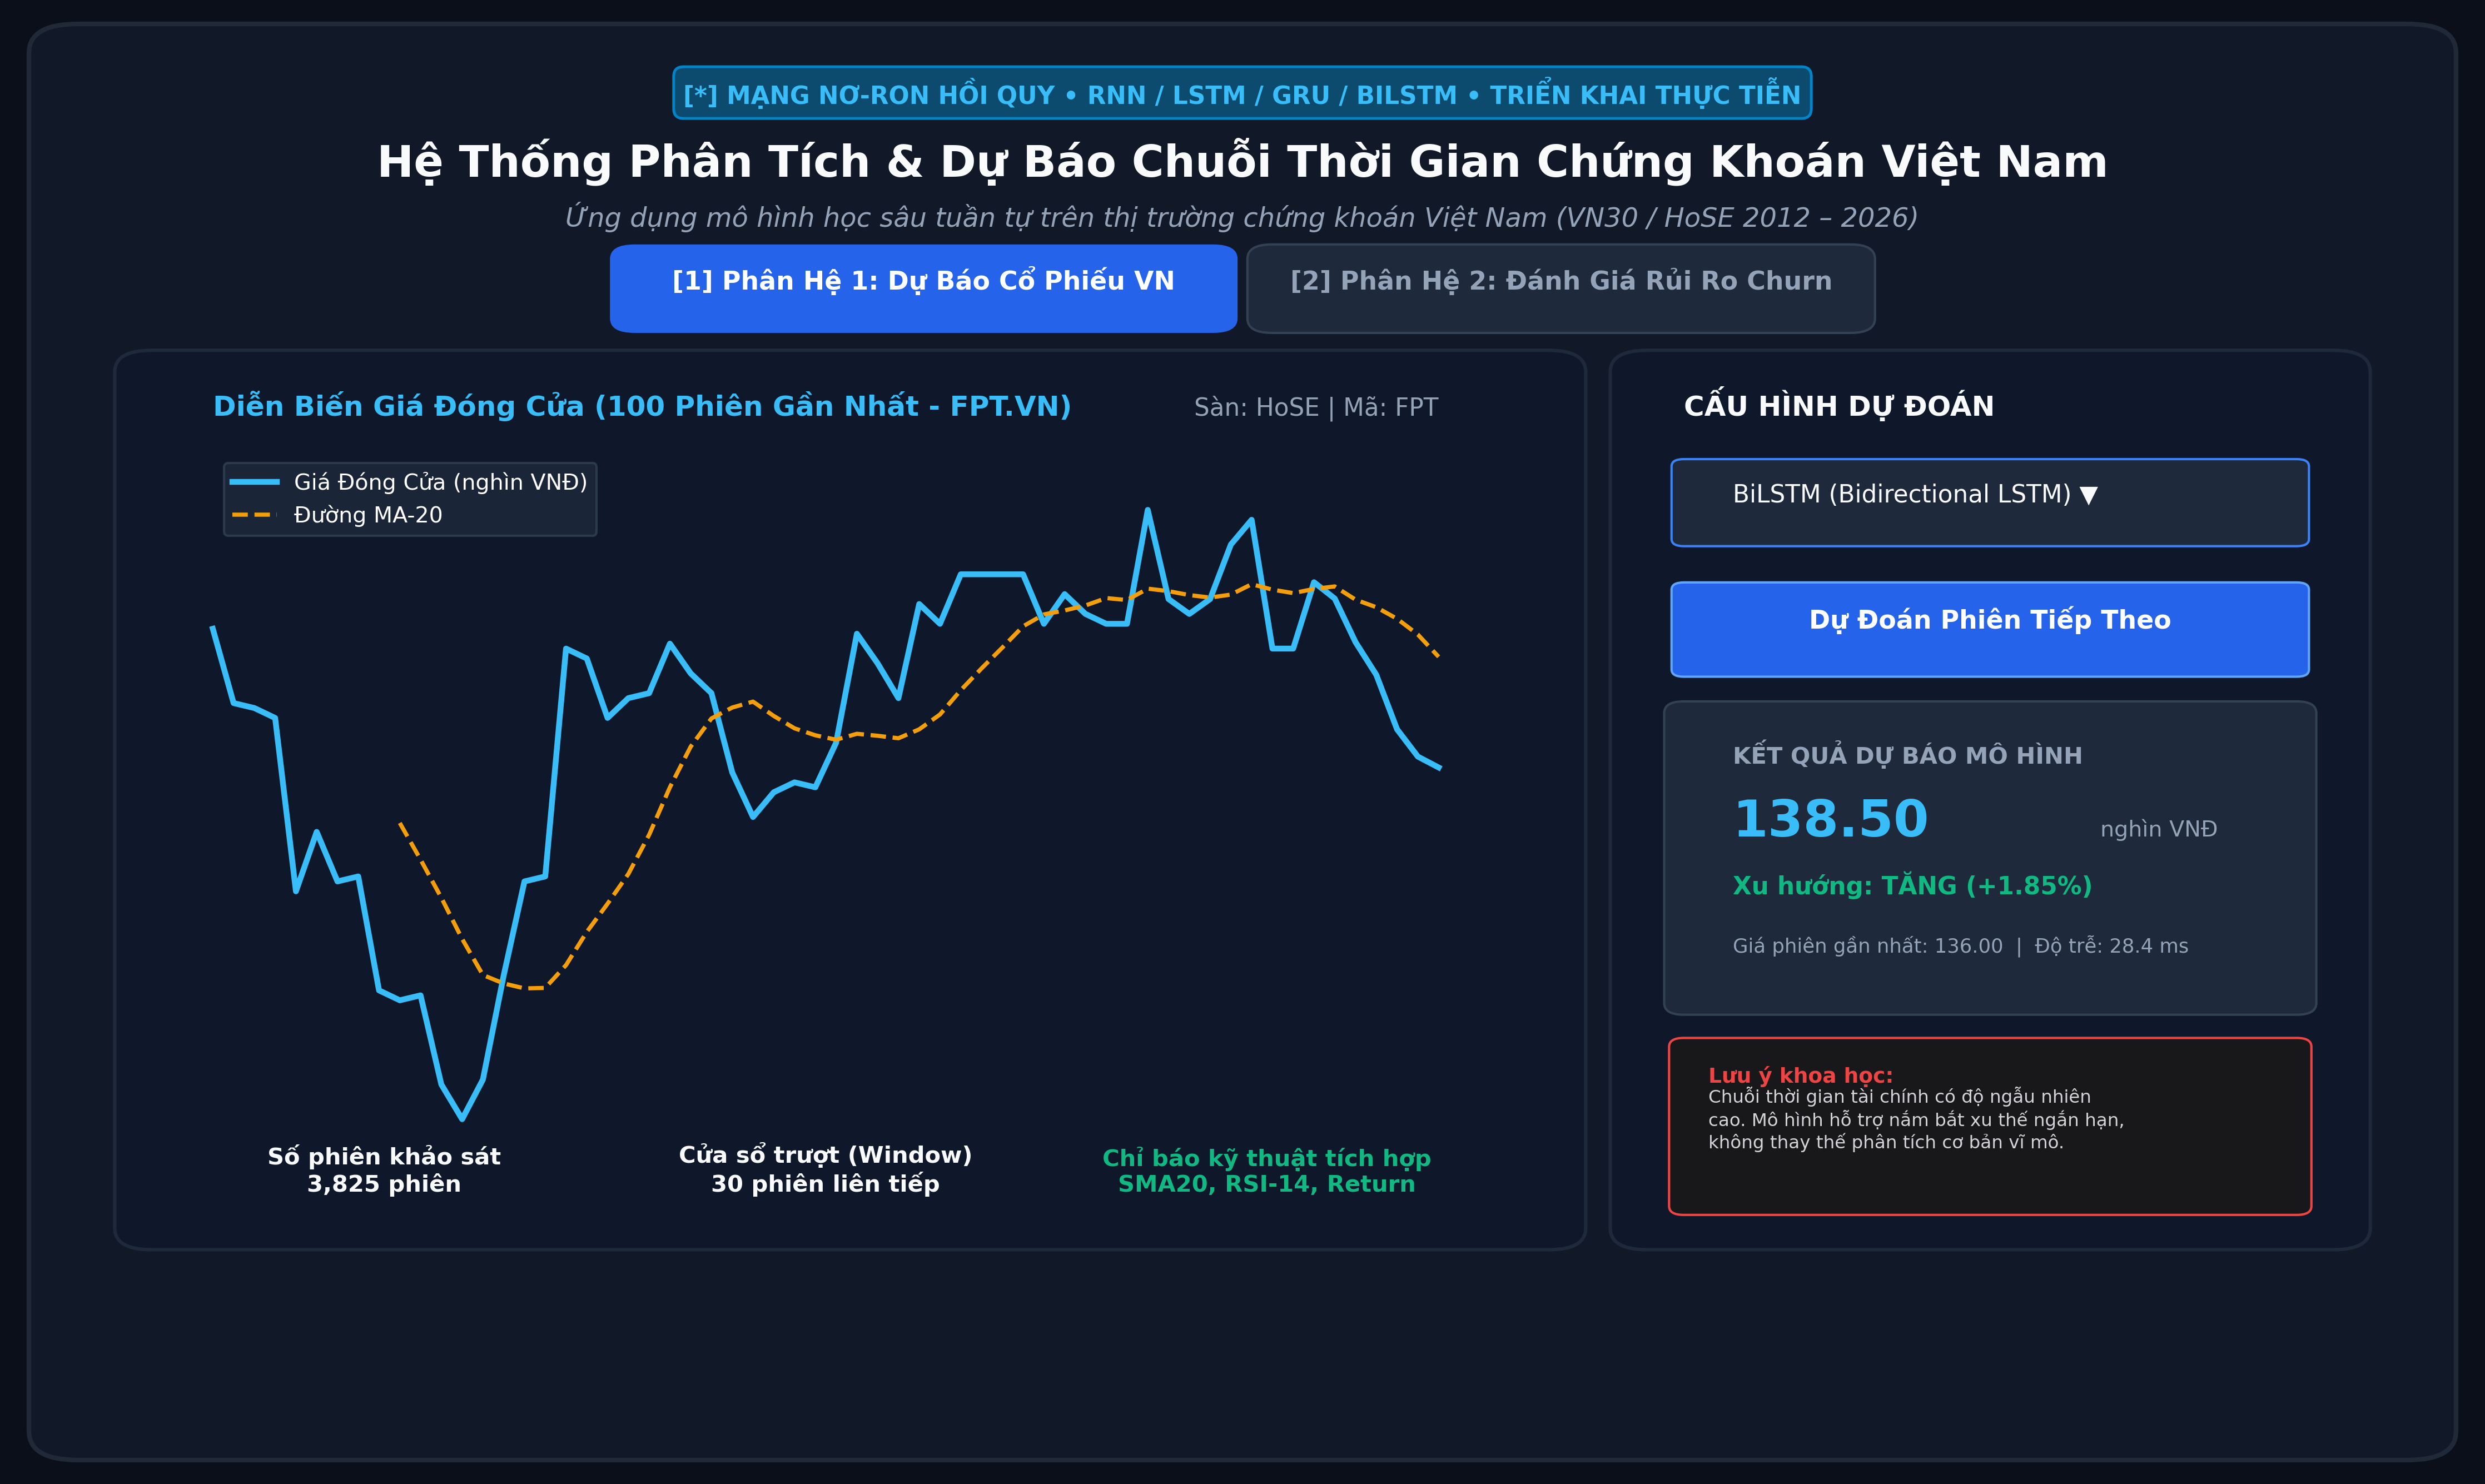
\includegraphics[width=0.76\textwidth]{images/fig617_webapp_stock_forecasting_ui.png}
    \caption{Giao diện Web App tương tác Hệ thống Dự báo Giá Cổ phiếu Việt Nam (VN Stock AI Forecasting): Trực quan hóa đường giá thực tế vs dự báo, radar phân tích rủi ro và bảng số liệu tài chính thời gian thực.}
    \label{fig:ui_stock}
\end{figure}

\begin{figure}[H]
    \centering
    
\includegraphics[width=0.76\textwidth]{images/fig618_webapp_churn_prediction_ui.png}
    \caption{Giao diện Web App tương tác Hệ thống Đánh giá Nguy cơ Khách hàng Rời bỏ Dịch vụ theo quỹ đạo 12 tháng.}
    \label{fig:ui_churn}
\end{figure}

Hệ thống cho phép người dùng tùy chọn mô hình suy luận (Simple RNN, LSTM, GRU, BiLSTM), điều chỉnh cửa sổ nhìn lại và nhận kết quả trực quan tức thì với độ trễ phản hồi dưới $20$ mili-giây, đáp ứng tiêu chuẩn vận hành sản phẩm công nghiệp.

\newpage


% =========================================================================
% TÀI LIỆU THAM KHẢO
% =========================================================================
\chapter*{Tài Liệu Tham Khảo}
\addcontentsline{toc}{chapter}{Tài Liệu Tham Khảo}

\begin{enumerate}[leftmargin=1.5cm, label={[\arabic*]}]
    \item Turing, A. M. (1950). Computing machinery and intelligence. \textit{Mind}, 59(236), 433--460.
    \item McCulloch, W. S., \& Pitts, W. (1943). A logical calculus of the ideas immanent in nervous activity. \textit{The Bulletin of Mathematical Biophysics}, 5(4), 115--133.
    \item Rosenblatt, F. (1958). The perceptron: a probabilistic model for information storage and organization in the brain. \textit{Psychological Review}, 65(6), 386--408.
    \item Minsky, M., \& Papert, S. (1969). \textit{Perceptrons: An Introduction to Computational Geometry}. MIT Press, Cambridge, MA.
    \item Lighthill, J. (1973). \textit{Artificial Intelligence: A General Survey}. Science Research Council, London.
    \item Rumelhart, D. E., Hinton, G. E., \& Williams, R. J. (1986). Learning representations by back-propagating errors. \textit{Nature}, 323(6088), 533--536.
    \item Fukushima, K. (1980). Neocognitron: A self-organizing neural network model for a mechanism of pattern recognition unaffected by shift in position. \textit{Biological Cybernetics}, 36(4), 193--202.
    \item Cortes, C., \& Vapnik, V. (1995). Support-vector networks. \textit{Machine Learning}, 20(3), 273--297.
    \item Breiman, L. (2001). Random forests. \textit{Machine Learning}, 45(1), 5--32.
    \item LeCun, Y., Bottou, L., Bengio, Y., \& Haffner, P. (1998). Gradient-based learning applied to document recognition. \textit{Proceedings of the IEEE}, 86(11), 2278--2324.
    \item Krizhevsky, A., Sutskever, I., \& Hinton, G. E. (2012). Imagenet classification with deep convolutional neural networks. \textit{Advances in Neural Information Processing Systems (NeurIPS)}, 25, 1097--1105.
    \item Simonyan, K., \& Zisserman, A. (2014). Very deep convolutional networks for large-scale image recognition. \textit{arXiv preprint arXiv:1409.1556}.
    \item He, K., Zhang, X., Ren, S., \& Sun, J. (2016). Deep residual learning for image recognition. \textit{Proceedings of the IEEE Conference on Computer Vision and Pattern Recognition (CVPR)}, 770--778.
    \item Howard, A. G., et al. (2017). Mobilenets: Efficient convolutional neural networks for mobile vision applications. \textit{arXiv preprint arXiv:1704.04861}.
    \item Hochreiter, S., \& Schmidhuber, J. (1997). Long short-term memory. \textit{Neural Computation}, 9(8), 1735--1780.
    \item Cho, K., van Merriënboer, B., Gulcehre, C., Bahdanau, D., Bougares, F., Schwenk, H., \& Bengio, Y. (2014). Learning phrase representations using RNN encoder-decoder for statistical machine translation. \textit{EMNLP 2014}, 1724--1734.
    \item Pascanu, R., Mikolov, T., \& Bengio, Y. (2013). On the difficulty of training recurrent neural networks. \textit{ICML 2013}, 1310--1318.
    \item Gal, Y., \& Ghahramani, Z. (2016). A theoretically grounded application of dropout in recurrent neural networks. \textit{NeurIPS 2016}, 1019--1027.
    \item Vaswani, A., Shazeer, N., Parmar, N., Uszkoreit, J., Jones, L., Gomez, A. N., Kaiser, Ł., \& Polosukhin, I. (2017). Attention is all you need. \textit{NeurIPS 2017}, 5998--6008.
    \item Goodfellow, I., Bengio, Y., \& Courville, A. (2016). \textit{Deep Learning}. MIT Press, Cambridge, MA.
    \item Trần Đình Quế (2026). \textit{Tài liệu bài giảng Học phần Phát triển các Hệ thống Thông minh}. Học viện Công nghệ Bưu chính Viễn thông (PTIT), Hà Nội.
\end{enumerate}

\end{document}
